\documentclass[PhD]{uclathes}

% Packages
%\usepackage[T1]{fontenc} % Allows for 8-bit font encoding
\usepackage{setspace} % Sets space between lines
\usepackage{animate,pdfpages} % Allow for animated figures, importing PDF figures, and converting EPS to PDF
\usepackage[space]{grffile} % Extended file name support for graphics
\usepackage{float} % Improved interface for floating objects
\usepackage{subcaption} % Allows for subfigures within figures
\usepackage{caption} % Captions in floating environments
\usepackage{array} % Extending the array and tabular environments
\usepackage{multirow} % Create tabular cells spanning multiple rows
\usepackage{gensymb} % Generic symbols for both text and math mode
\usepackage{amsmath,amssymb,amsfonts,amsthm,mathrsfs,mathtools,accents} % Various packages for math typesetting
\usepackage{adjustbox,relsize} % Set font size relative to the current font size
\usepackage[notrig]{physics} % Physics symbols and units
\usepackage{siunitx} % Physics units
\usepackage{cancel,slashed} % Place lines through math and slashes through characters
\usepackage{xparse} % Generic document command parser
\usepackage{tikz,tikz-3dplot,circuitikz,pgfplots,tikz-cd,tikz-feynman} % Drawing environments
\usepackage{centernot} % Centered \not command
\usepackage{xcolor} % Color extensions for LaTeX and pdfLaTeX
\usepackage{listings} % Typeset text in WYSIWYG style and source code listings
\usepackage{fancyvrb} % Sophisticated verbatim text
\usepackage{lastpage} % Reference last page for Page N of M type footers
\usepackage[percent]{overpic} % Combine LaTeX commands over included graphics
\usepackage{empheq} % Emphasizing equations
\usepackage{comment} % Allows for commenting out large blocks of code
\usepackage[title]{appendix} % Customization of appendices
\usepackage{simpler-wick} % Allows for Wick contractions
\usepackage[htt]{hyphenat} % Enables hyphenation in \texttt environments
\usepackage{url} % Allows for \path command for long file paths
\usepackage[hidelinks,colorlinks=false]{hyperref} % Allow for hyperlinks
\usepackage{bookmark} % Automatically create bookmarks
\usepackage{xspace} % Allows for \xspace command to check if a space is needed
\usepackage{cite} % Makes citations with multiple references look better


% Configure TikZ
% Load TikZ libraries
\usetikzlibrary{patterns,plotmarks,arrows,decorations.pathmorphing,decorations.markings,shapes.geometric,calc,shapes.misc,3d}

\tikzset{>=latex}
\tikzset{pics/particle/.style n args={6}{code={
			\draw[rounded corners,fill=#1] (-1,-1) rectangle (1,1);
			\node at (0,0) [scale=2,anchor=mid] {#2};
			\node at (0,-0.8) [scale=0.8,anchor=mid] {#3};
			\node at (-1,0.8) [scale=0.5,anchor=mid west] {#4};
			\node at (-1,0.5) [scale=0.5,anchor=mid west] {#5};
			\node at (-1,0.2) [scale=0.5,anchor=mid west] {#6};
}}}

% Commands
\def\eqheight{-\the\dimexpr\fontdimen22\textfont2\relax}

% Configure listings
% Command for setting number of lines for code
\newlength{\numwidth}
\makeatletter
\newcommand{\setlinenum}[1]
{
	\setlength{\numwidth}{\widthof{\footnotesize{\lst@numberstyle{#1}}}}
	\def\lst@PlaceNumber{%
		\makebox[\numwidth+1em][l]{%
			\makebox[\numwidth][r]{\footnotesize\lst@numberstyle{\thelstnumber}}
		}
	}
}
\makeatother
\setlinenum{9} % Set to 9 lines of code by default

% Default style
\lstdefinestyle{default}
{
	showstringspaces=false,
	breaklines=true,
	frame=lines,
	basicstyle=\footnotesize\ttfamily,
	numbers=none,
}

% Plain style
\lstdefinestyle{plain}
{
	showstringspaces=false,
	breaklines=true,
	basicstyle=\footnotesize\ttfamily,
	numbers=none,
}

% LaTeX style
\lstdefinestyle{latex}
{
	language=LaTeX,
	showstringspaces=false,
	breaklines=true,
	frame=lines,
	basicstyle=\footnotesize\ttfamily,
	numberstyle=\footnotesize\ttfamily,
}

% Python style
\lstdefinestyle{python}
{
	language=Python,
	showstringspaces=false,
	breaklines=true,
	frame=lines,
	basicstyle=\footnotesize\ttfamily,
	numberstyle=\footnotesize\ttfamily,
}

% C++ style
\lstdefinestyle{cpp}
{
	language=C++,
	showstringspaces=false,
	breaklines=true,
	frame=lines,
	basicstyle=\footnotesize\ttfamily,
	numberstyle=\footnotesize\ttfamily,
}


% Configure captions
\captionsetup[table]{font={stretch=1.5}}
\captionsetup[figure]{font={stretch=1.5}}

% Configure itemize layers
\renewcommand{\labelitemii}{\ensuremath{\circ}}

% Enable bold math in section titles
\makeatletter
\g@addto@macro\bfseries{\boldmath}
\makeatother

% Commands
\renewcommand\qedsymbol{$\blacksquare$} % Change QED symbol to solid black box
\newcommand\numberthis{\addtocounter{equation}{1}\tag{\theequation}} % Number equations in align* environments

\sisetup{inter-unit-product=\ensuremath{{}\cdot{}}} % Change symbol for products of physical units
\renewcommand{\unit}{\ \si} % Define physical unit command with proper spacing
\DeclareSIUnit\clight{\text{\ensuremath{c}}} % Redefine speed of light so that it has no subscript

% Redefine command for unit vectors to add space
\let\oldvu\vu
\makeatletter
\renewcommand{\vu}{\@ifstar{\mathop{}\!\oldvu*}\mathop{}\!\oldvu}
\makeatother

% Create spacing for equals sign in align environments
\newcommand{\equad}{\mathrel{\phantom{=}}}

% Alphabet for blackboard bold numbers
\newcommand{\bbfamily}{\fontencoding{U}\fontfamily{bbold}\selectfont}
\DeclareMathAlphabet{\mathbbold}{U}{bbold}{m}{n}

\newcommand{\lumi}{\mathcal{L}} % Luminosity
\newcommand{\intlumi}{\mathcal{L}_\mathrm{int}} % Integrated luminosity
\newcommand{\pt}{\ensuremath{p_\mathrm{T}}\xspace} % Transverse momentum


\title{
	Search for Long-Lived Particles Decaying to Photon Pairs in Rare Higgs Boson Decays using 13 TeV Proton-Proton Collisions at the Compact Muon Solenoid
}

\author{Tyler Christopher Lam}
\department{Physics}
\degreeyear{2024}

\chair{Michalis Bachtis}
\member{Davlid Saltzberg}
\member{Jay Hauser}
\member{Thomas Dumitrescu}
\dedication{
	\textit{
		To my parents, Jean and Bobby, for their love and support from across the country
	}
}

\acknowledgments{
First and foremost, no one has contributed more to my success as a graduate student than my advisor, Michalis Bachtis. The first summer I spent researching for him cemented my desire to study experimental particle physics. From there, his dedication, enthusiasm, and mentorship were indispensable during my journey through graduate school.  I do not know of any advisor who is more available to their students and is more willing to perform hands-on work to help in a project. Thank you for everything, Michalis.

More thanks goes to the current and former members of the UCLA CMS research group. Thank you to my former officemates David Hamilton and Maxx Tepper; our workplace shenanigans gave me something to look forward to during slow days at work. I would also like to thank the other CMS graduate students from when I arrived at UCLA: Brent Stone, Will Nash, and Chris Schnaible for welcoming me into the group and our countless thought-provoking lunch discussions. Lastly, a thanks to the remaining graduate students, engineers, and postdocs Gael Flores-Avila, Antonett Prado, Abhishek Datta, Elisabetta Manca, Joseph Carlson, David Gotler, Alex Tan, and Delano Campos for making the office an enjoyable place to work.

My time at UCLA has been marked by countless friendships with students outside of the CMS research group as well. No words can express how important my former roommates Adam Trapp and Kyle Ferguson were towards maintaining my sanity during a global pandemic. Despite everything, I look back on our many (mis)adventures and remember this time fondly. You have been such an integral part of my time at UCLA that, to avoid repetition, I ask that put yourselves in any of the following thanks that apply to you. In a similar vein, thank you to Ronald Lopez and Rick Mebane for the weekly tennis sessions, which gave me an excuse to go outside during the lockdown. I would also like to thank Eric Cropp, Eddie Chang, Lukas Lindwasser, and Pratik Sathe for turning our comprehensive exam study group into a food-centric outing group.  To my friends that I have bonded with on the bouldering wall, I would like to thank Tony Pahl, Abhijah Simon, Akash Gupta, Rory Bentley, Will Flanagan, and Wes Armstrong. Finally, for making after-work and weekend board game nights fun I would like to thank Sarah Chase, Henry Wong, and Phil Travis.

Beyond UCLA, I would like to thank my parents, Bobby and Jean, who eventually learned not to ask a graduate student when they will graduate. My career as a physicist would never have been possible without them. Thank you to my sibling Ira for being a consistent moral and political compass. Additional thanks to Tor Raubenheimer -- my uncle, Stanford professor, and physicist at SLAC -- who inspired me to study physics in middle school when he joined our family. Last, but by no stretch of the imagination least, thank you to Levina Lin for being an unending source of stability and support over the last few years.

This thesis includes material that is based upon work supported by the U.S. Department of Energy under award number DE-SC0009937.
}

\vitaitem{2017}
{
	B.S\ (Physics) and B.A.\ (Mathematics),
	University of Virginia
}

\vitaitem{2017-2018}
{
	Teaching Assistant,
	Department of Physics and Astronomy,
	UCLA,
	Los Angeles, California
}

\vitaitem{2018}
{
	M.S.\ (Physics)
	UCLA
}

\vitaitem{2018-2024}
{
	Graduate Research Assistant,
	Department of Physics and Astronomy,
	UCLA
}

\abstract{
This thesis describes the search for rare Standard Model (SM) Higgs boson decays to long-lived scalar bosons ($\Phi$) decaying to photon pairs using data collected by the Compact Muon Solenoid (CMS) detector at the Large Hadron Collider. The data were collected from 2016, 2017, and 2018 proton-proton collisions at center-of-mass energy of $\sqrt{s}=13\TeV$ and correspond to an integrated luminosity of $138\unit{fb^{-1}}$. Events are triggered using the leptonic decays of the \PZ boson produced in association with the SM Higgs boson. Although the CMS electromagnetic calorimeter has limited vertex reconstruction capabilities for photons, this analysis utilizes a novel reconstruction technique using kinematic constraints to calculate the displaced vertices of the diphotons. Signal is extracted using a counting-based maximum-likelihood approach in bins of the diphoton vertex \lxy and the invariant photon mass. Results are interpreted in terms of upper limits on branching ratios $\mathcal{BR}(\PH\to\Phi\Phi)\times\mathcal{BR}(\Phi\to\PGg\PGg)$ and in terms of the model independent production cross section $\sigma(\PZ+\Phi\Phi)\times\mathcal{BR}(\Phi\to\PGg\PGg)$. No significant excess above SM expectation is observed.
}

\begin{document}

\makeintropages

% !TEX = root../thesis.tex

\chapter{Introduction}
\label{chap:intro}
% !TEX = root../thesis.tex

\chapter{The Standard Model and Motivations for Displaced Photons}
\label{chap:theory}
In this chapter, we present an overview of the Standard Model (SM) -- the best current description of the fundamental constituents of matter and the interactions between them. We begin with a brief description of the SM particles, followed by an outline of the mechanism that determines particle lifetimes. This establishes the groundwork to discuss the Higgs boson its relation to long-lived, beyond the standard model particles that motivate the $\PH\to\Phi\Phi\to\PGg\PGg+X$ analysis presented in chapter~\ref{chap:ana}.

\section{Elementary Particles in the Standard Model} \label{sec:SM}
The Standard Model is a quantum field theory that describes interactions between fundamental particles (see appendix~\ref{sec:sm_theory_qft} for a description of the mathematical formalism). According to the SM, all matter is composed of spin-1/2 particles known as fermions with forces that interact via fields mediated by spin-1 gauge bosons. Of the four forces -- gravity, electromagnetic, weak, and strong -- the SM provides a description of all but gravity. The spin-1/2 fermions can be divided into three generations of increasing mass, with each generation divided into a quark doublet and lepton doublet. The gauge bosons are composed of the photon ($\PGg$) which mediates the electromagnetic force, the \PZ and \PWpm bosons which mediate the weak force, and 8 gluons (\Pg) which mediate the strong force. The \PZ and \PW bosons gain mass through a process known as the Higgs mechanism, which predicts the existence of a scalar boson \PH known as the Higgs boson. This process is presented in detail in section~\ref{sec:sm_theory_higgs}. Figure~\ref{tab:SM} shows the mass, charge, and spin of the fermions grouped by generation, the gauge bosons, and the Higgs boson. Each fermion has an associated antiparticle with identical spin and mass but opposite electrical charge.

\begin{figure}[htb!]
	\centering
	% !TEX = root../../thesis.tex

% Colors from https://latexcolor.com/
\definecolor{aqua}{rgb}{0.5, 1.0, 1.0}
\definecolor{spring}{rgb}{0..65, .99, 0.0}
\definecolor{brick}{rgb}{.8, .25, .33}
\definecolor{ube}{rgb}{0.82, 0.62, 0.91}

\begin{tikzpicture}
	\coordinate (u) at (0,0);
	\coordinate (d) at (0, -2.15);
	\coordinate (c) at (2.15, 0);
	\coordinate (s) at (2.15, -2.15);
	\coordinate (t) at (4.3, 0);
	\coordinate (b) at (4.3, -2.15);
	\coordinate (e) at (0, -4.3);
	\coordinate (mu) at (2.15, -4.3);
	\coordinate (tau) at (4.3, -4.3);
	\coordinate (ne) at (0, -6.45);
	\coordinate (nmu) at (2.15, -6.45);
	\coordinate (ntau) at (4.3, -6.45);
	\coordinate (glu) at (6.75, 0);
	\coordinate (g) at (6.75, -2.15);
	\coordinate (z) at (6.75, -4.3);
	\coordinate (w) at (6.75, -6.45);
	\coordinate (h) at (9.20, 0);
	
	% quarks
	\draw pic at (u) {particle={aqua!50}{$\PQu$}{up}{$2.16\MeVcc$}{$2/3$}{$1/2$}}; %Up quark
	\draw pic at (d) {particle={aqua!50}{$\PQd$}{down}{$4.70\MeVcc$}{$-1/3$}{$1/2$}}; % Down quark
	\draw pic at (c) {particle={aqua!50}{$\PQc$}{charm}{$1.27\GeVcc$}{$2/3$}{$1/2$}}; %Charm
	\draw pic at (s) {particle={aqua!50}{$\PQs$}{strange}{$93.5\MeVcc$}{$-1/3$}{$1/2$}}; %Strange
	\draw pic at (t) {particle={aqua!50}{$\PQt$}{top}{$172.57\GeVcc$}{$2/3$}{$1/2$}}; %Top
	\draw pic at (b) {particle={aqua!50}{$\PQb$}{bottom}{$4.183\GeVcc$}{$-1/3$}{$1/2$}}; %Bot
	
	% leptons
	\draw pic at (e) {particle={spring!35}{$\Pe$}{electron}{$511\keVcc$}{$-1$}{$1/2$}};
	\draw pic at (mu) {particle={spring!35}{$\PGm$}{muon}{$105.66\MeVcc$}{$-1$}{$1/2$}}; 
	\draw pic at (tau) {particle={spring!35}{$\PGt$}{tau}{$1.776\GeVcc$}{$-1$}{$1/2$}}; 
	\draw pic at (ne) {particle={spring!35}{$\PGne$}{\Pe neutrino}{$<1.1\eVcc$}{$0$}{$1/2$}};
	\draw pic at (nmu) {particle={spring!35}{$\PGnGm$}{\PGm neutrino}{$<0.17\MeVcc$}{$0$}{$1/2$}};
	\draw pic at (ntau) {particle={spring!35}{$\PGnGt$}{\PGt neutrino}{$<18\MeVcc$}{$0$}{$1/2$}};	
	
	% gauge bosons
	\draw pic at (glu) {particle={brick!30}{$\Pg$}{gluon}{$0$}{$0$}{$1$}};
	\draw pic at (g) {particle={brick!30}{$\PGg$}{photon}{$0$}{$0$}{$1$}};
	\draw pic at (z) {particle={brick!30}{$\PZ$}{Z boson}{$91.188\GeVcc$}{$0$}{$1$}};
	\draw pic at (w) {particle={brick!30}{$\PW$}{W boson}{$80.37\GeVcc$}{$\pm1$}{$1$}};
	
	% Higgs
	\draw pic at (h) {particle={ube!50}{$\PH$}{Higgs boson}{$125.2\GeVcc$}{0}{0}};
	
	% Labels
	\node at ($(u)+(-1, 0.8)$) [anchor=mid east, scale=0.6] {mass};
	\node at ($(u)+(-1, 0.5)$) [anchor=mid east, scale=0.6] {charge};
	\node at ($(u)+(-1, 0.2)$) [anchor=mid east, scale=0.6] {spin};
	
	\node at ($(u)+(0, 1.35)$) {I};
	\node at ($(c)+(0, 1.35)$) {II};
	\node at ($(t)+(0, 1.35)$) {III};	
	%\node at ($(c)+(0, 1.9)$) {Generations};
	\node at ($(u)+(-1,1.35)$) [anchor=east, scale=0.75] {Generation};
	
	\node at ($(d)+(-1.35, -1)$) [rotate=90,anchor=mid west, text=aqua!60!black] {Quarks};
	\node at ($(ne)+(-1.35, -1)$) [rotate=90,anchor=mid west, text=spring!60!black] {Leptons};
	\node at ($(w)+(1.35, -1)$) [rotate=90,anchor=mid west, text=brick!60!black] {Gauge Bosons};
\end{tikzpicture}

	\caption[Table of all Standard Model particles, divided by generation and particle type. Each particle is labeled with its mass, charge, spin, and symbol. Quarks are shown in blue, leptons in green, gauge bosons in red, and the Higgs boson in purple.]{Table of all Standard Model particles, divided by generation and particle type. Each particle is labeled with its mass, charge, spin, and symbol. Quarks are shown in blue, leptons in green, gauge bosons in red, and the Higgs boson in purple. Values taken from~\cite{Workman:2022ynf}.}
	\label{tab:SM}
\end{figure}

\subsection{Fermions} \label{sec:sm_quarks}
Quarks are fermions that interact with the strong, weak, and electromagnetic force. They are found exclusively in bound states known as hadrons. The two main types of hadrons are quark-antiquark pairs called mesons or three quark (or three antiquark) configurations known as baryons. For example, protons, the most commonly known baryons, are composed of two up quarks and one down quark (\PQuns\PQuns\PQdns), and the \PGpp is a meson composed of an up quark and a down antiquark (\PQuns\PAQdns). Each column of quarks in table~\ref{tab:SM} forms a doublet, with the upper quark having charge $+2/3$ while the lower quark has charge $-1/3$. Thus mesons can have charge 0 or $\pm$1 and baryons can have charge 0, $\pm$1, or $\pm$2.

Due to their interaction with the strong force, quarks carry one of three ``color'' charges of either red, blue, or green (or antired, antiblue, or antigreen). Although it is not theoretically required, it has been experimentally shown that quarks must always exist in a colorless bound state. Baryons must have one quark of each color (or anti-color), and mesons must consist of color-anticolor pairs. This property is known as color confinement.

Leptons are fermions consisting of three charged particles -- the electron, muon, and tau (\Pe, \PGm, and \PGt) -- and three corresponding neutral particles (\PGne, \PGnGm, and \PGnGt) called neutrinos. The charged leptons interact through both the electromagnetic and weak force, while the neutrinos interact only through the weak force. The lepton and neutrino doublets are intrinsically linked through the weak force. Neutrinos have extremely small masses compared to the other massive SM particles, and can undergo oscillations between flavors.

\subsection{Bosons} \label{sec:sm_bosons}
The gauge bosons are the spin-1 mediators of the electromagnetic, weak, and strong forces. The photon is the massless mediator of the electromagnetic force and couples to charged particles. Since they do not carry electric charge, photons do not directly interact with other photons. On the other hand, gluons, which are the massless mediators for the strong force, carry two color charges and can therefore interact with other gluons. Lastly, the \PZ and \PWpm bosons are the mediators of the weak force and can interact with all fermions as well as each other.

The Higgs boson is the only currently known scalar boson. In the SM, the \PZ and \PWpm bosons as well as all fermions are required to be massless due to various symmetry requirements. The Higgs mechanism, through a process known as spontaneous symmetry breaking, allows these particles to acquire non-zero mass without violating conservation laws. In this sense, the Higgs boson is said to give masses to the particles. The Higgs boson couples to any particle with mass, which includes itself, the aforementioned \PZ and \PWpm bosons, and all SM fermions.

\section{Fermi's Golden Rule and Particle Lifetimes} \label{sec:theory_fermi}
One of the key results from quantum field theory relates the interactions between particles to the rate at which they decay. Fermi's Golden Rule, which is more commonly known for describing transition rates using perturbation theory in QM, can be applied to Lorentz invariant particle decays~\cite{pdg2024}. For the decay $1\to2+3+...+n$, the partial decay rate is given by
\begin{equation}
	\dd{\Gamma}=\frac{(2\pi)^4}{2m_1}|\mathcal{M}|^2\dd{\Phi_n(p_1,p_2,...,p_n)}
\end{equation}
where $\mathcal{M}$ is the matrix element of the decay determined by the coupling strength and the interaction term of the initial and final states in the Lagrangian and $\dd{\Phi_n(p_1,p_2,...,p_n)}$ is a differentiable element of the phase space given by
\begin{equation}
	\dd{\Phi_n(p_1,p_2,...,p_n)}=\delta^4(p_1-\sum_{i=2}^n p_i)\prod_{i=2}^n\frac{\dd[3]{p_i}}{(2\pi)^32E_i}
\end{equation}
For a two body decay, integrating over the phase space gives a total decay rate of
\begin{equation}
	\Gamma=\frac{|p_i|}{8\pi m_1^2}|\mathcal{M}|^2
\end{equation}
This is the decay rate for the specific decay mode $1\to2+3$. One parameter of interest is the total decay rate for all processes, given by $\Gamma=\sum_{i}\Gamma_i$, where $i$ sums over all possible decay modes. Particles decays follow a Poisson distribution, meaning that the decay probability is independent of how long the particle has existed. The probability for a particle with total decay rate $\Gamma$ to decay after a time $t$ is given by
\begin{equation}
	\mathcal{P}(t\,|\,\Gamma)=\Gamma e^{-\Gamma t}=\frac{1}{\tau}e^{-t/\tau}
\end{equation}
where the mean lifetime $\tau=1/\Gamma$.

For a two body decay, the invariant mass distribution of the decay products forms a peak around the invariant mass of the parent particle, which is often referred to as a \textit{resonance}. The shape of this distribution is known as a Breit-Wigner distribution and is related to the decay rate. Suppose the total Hamiltonian of the system is $H=H_0+H'$, where $H_0$ has energy eigenstates and eigenvalues given by $H_0\ket{\psi_n}=E_n\ket{\psi_n}$ and $H'$ is treated as a small perturbation. Using first order perturbation theory, if the initial particle begins in state $\psi_i$, the probability to measure the parent particle in a state with energy $E_j$ is given by
\begin{equation}
	\left|c_j(t)\right|^2=\frac{\left|\bra{\psi_j}H\ket{\psi_i}\right|^2}{(E_j-E_i)^2+\Gamma^2/4}
\end{equation}
This curve has a peak at $E_i$ and a full width at half maximum (FWHM) equal to $\Gamma$. As a consequence, the longer a particle's lifetime the broader the peak in its mass distribution. Although it appears the energy of the system changed after the decay, conservation of energy is not violated as the initial state $\ket{\psi_i}$ is not an eigenstate of the full Hamiltonian and does not have a well defined energy~\cite{breitwigner}. Particles can have long lifetimes for several factors, such as phase space restrictions or suppressed decays in the matrix element.

\section{Motivations for Long Lived Scalar Bosons} \label{sec:BSM}
Despite the success of the Standard Model as the most accurate and precise description of fundamental particles and their interactions, there exist substantial shortcomings that remain unanswered. Section~\ref{sec:theory_motivation} will outline a few of the outstanding problems with the Standard Model, with potential solutions involving long-lived particles presented in section~\ref{sec:LLPs}.

\subsection{Beyond the Standard Model} \label{sec:theory_motivation}
There exists numerous observed and theoretical phenomena that motivates the need for physics beyond the Standard Model. Dark matter, which is required to explain the rotational velocity of distant galaxies~\cite{zwicky_dm}, must be a massive, neutral, stable particle -- which currently does not exist in the Standard Model. Another notable absence, as mentioned in section~\ref{sec:SM}, is a description of the gravitational force. Additionally, the Standard Model assumes that neutrinos are massless (and thus only exist as left-handed fermions), but experimental observations of neutrino flavor oscillations indicate that the neutrinos must have non-zero mass. Even the exact nature of the Higgs boson is unknown, as the potential for spontaneous symmetry breaking (see appendix~\ref{sec:sm_theory_beh}) is not unique and merely the simplest form that produces three massive and one massless gauge bosons. This section will cover a few of the most relevant issues with the Standard Model as they pertain to this dissertation.

\subsubsection{Baryon Asymmetry} \label{sec:baryon_asymmetry}
It is assumed that matter and antimatter were originally created in equal quantities, yet all the baryons in the universe are composed of matter instead of antimatter. The critical phenomena to create this asymmetry are baryon number violation, periods of thermal fluctuation, and CP violation, meaning the rate for a given process is different from the rate of the CP-conjugate process~\cite{Sakharov:1967dj}. The standard model does contain the necessary mechanisms for CP violation through phase factors in the mixing matrices between flavor and mass eigenstates, as demonstrated by Kaon regeneration and neutrino oscillations. However, the amount of CP violation allowed by the Standard Model only accounts for a minuscule fraction of this asymmetry while the rest remains unexplained~\cite{Peskin2002}. One leading theory is Electroweak Baryogenesis (EWBG), a process where a first-order electroweak phase transition occurs as the early universe cools to $T<100\GeV$ which results in an excess of baryonic matter~\cite{ewbg1,ewbg2}.

\subsubsection{The Hierarchy Problem} \label{sec:hierarchy}
The energy at which gravitational effects become dominant for particle physics experiments is known as the Planck mass and can be calculated using fundamental constants as
\begin{equation}
	m_\text{Pl}=\sqrt{\frac{\hbar c}{G}}\approx10^{19}\GeVcc
\end{equation}
While this value does not contradict the Standard Model, it indicates experiments that could probe this energy scale are well out of reach for modern particle accelerators. It also creates a hierarchy problem regarding the mass of the Higgs boson that arises when accounting for the corrections to the Higgs boson mass through renormalization. Using loop corrections, one must choose a momentum cutoff $\Lambda_\text{UV}$ to evaluate the integrals that contribute to the mass of the Higgs boson~\cite{Peskin:1995ev}. The ``natural'' choice, if the Standard Model is believed to be valid for all mass scales, would be to take $\Lambda_\text{UV}\to m_\text{Pl}$. However, these corrections go as $O(\Lambda_\text{UV}^2)$, causing the calculated Higgs boson mass to quickly grow past the observed value.

To prevent these divergences requires the parameters of the standard model to be manipulated (or ``fine-tuned'') in order to produce the observed Higgs boson mass. This fine-tuning is allowed by the Standard Model, as the Higgs vacuum expectation value is a free parameter, but there are several theoretical models that remove the need for fine-tuning entirely~\cite{hierarchy}. Supersymmetry, for example, theorizes every fermion has a supersymmetric bosonic counterpart (and every boson a fermionic counterpart) and results in the loop contributions perfectly canceling term by term~\cite{susy}.

\subsubsection{Muon Anomalous Magnetic Moment} \label{sec:gminus2}
The Dirac equation predicts the muon to have an anomalous magnetic moment given by
\begin{equation}
	\mathbf{M}=g_\mu\frac{e}{2m_\mu}\mathbf{S}
\end{equation}
where $\mathbf{S}$ is the spin angular momentum, $e$ is the elementary charge, $m_\mu$ is the mass of the muon, and $g_\mu$ is the muon g-factor. By using the tree level interaction from the QED Lagrangian, one can calculate that the first order value of $g_\mu=2$~\cite{gminus2_slides}. However, higher order interactions shown in figure~\ref{fig:muon_magnetic_moment} contribute very small corrections to the g-factor, causing the theoretical value of $g_\mu$ to be very slightly more than 2.
\begin{figure}[htb!]
	\begingroup
	\tikzset{every picture/.style={scale=0.5}}
	% !TEX = root = ../../thesis.tex
\begin{tikzpicture}
	\begin{feynman}
		\coordinate[label=left:$\PGm$] (mu1) at (0,0);
		\coordinate[label=right:$\PGm$] (mu2) at (8,0);
		\coordinate (v1) at (2,1);
		\coordinate (v2) at (6,1);
		\coordinate (v3) at (4,{1+2*sqrt(3)});
		\coordinate[label=above:$\PGg$] (g1) at (4,6);
		\draw[fermion] (mu1) -- (v1);
		\draw[fermion] (v1) -- (v3);
		\draw[fermion] (v3) -- (v2);
		\draw[fermion] (v2) -- (mu2);
		\draw[photon] (v3) -- (g1);
		\draw[photon] (v1) -- (v2);
		
		\node[label={left:$\PGm$}] at (3,{1+sqrt(3)}){};
		\node[label={below:$\PGg/\PZ$}] at (4, 1){};
		\node[label={right:$\PGm$}] at (5, {1+sqrt(3)}){};
	\end{feynman}
\end{tikzpicture}
	% !TEX = root = ../../thesis.tex
\begin{tikzpicture}
	\begin{feynman}
		\coordinate[label=left:$\PGm$] (mu1) at (0,0);
		\coordinate[label=right:$\PGm$] (mu2) at (8,0);
		\coordinate (v1) at (2,1);
		\coordinate (v2) at (6,1);
		\coordinate (v3) at (4,{1+2*sqrt(3)});
		\coordinate[label=above:$\PGg$] (g1) at (4,6);
		\draw[fermion] (mu1) -- (v1);
		\draw[boson] (v1) -- (v3);
		\draw[boson] (v3) -- (v2);
		\draw[fermion] (v2) -- (mu2);
		\draw[photon] (v3) -- (g1);
		\draw[fermion] (v1) -- (v2);
		
		\node[label={left:$\PW$}] at (3,{1+sqrt(3)}){};
		\node[label={below:$\PGnGm$}] at (4, 1){};
		\node[label={right:$\PW$}] at (5, {1+sqrt(3)}){};
	\end{feynman}
\end{tikzpicture}
	% !TEX = root = ../../thesis.tex
\begin{tikzpicture}
	\begin{feynman}
		\coordinate[label=left:$\PGm$] (mu1) at (0,0);
		\coordinate[label=right:$\PGm$] (mu2) at (8,0);
		\coordinate (v1) at (2,1);
		\coordinate (v2) at (6,1);
		\coordinate (v3) at (4,{1+2*sqrt(3)});
		\coordinate (v4) at (3.25,1);
		\coordinate (v5) at (4.75,1);
		\coordinate[label=above:$\PGg$] (g1) at (4,6);
		\draw[fermion] (mu1) -- (v1);
		\draw[fermion] (v1) -- (v3);
		\draw[fermion] (v3) -- (v2);
		\draw[fermion] (v2) -- (mu2);
		\draw[photon] (v3) -- (g1);
		\draw[photon] (v1) -- (v4);
		\draw[photon] (v5) -- (v2);
		
		\draw[fermion] (4.75,1) arc (0:180:0.75);
		\draw[fermion] (3.25,1) arc (180:360:0.75);
		\node[label={left:$\PGm$}] at (3,{1+sqrt(3)}){};
		\node[label={right:$\PGm$}] at (5, {1+sqrt(3)}){};
		\node[label={below:$\PGg$}] at (2.625, 1){};
		\node[label={below:$\PGg$}] at (5.375,1){};
		\node[label={below:$\PQq$}] at (4, .25){};
		\node[label={above:$\PAQq$}] at (4, 1.75){};
	\end{feynman}
\end{tikzpicture}
	\endgroup
	\caption[First-order QED and lowest-order weak/hadronic contributions to the muon anomalous magnetic moment.]{First-order QED and lowest-order weak/hadronic contributions to the muon anomalous magnetic moment.}
	\label{fig:muon_magnetic_moment}
\end{figure}
The deviation of $g_\mu$ from 2 is parameterized using the magnetic anomaly defined as
\begin{equation}
	a_\mu\equiv\frac{g_\mu-2}{2}
\end{equation}
Calculating the magnetic anomaly through 5 loops in QED corrections, 2 loops in electroweak corrections, and 3 loops in hadronic corrections gives $a_\mu^\text{SM}=116\,591\,810(1)(40)(18)\times10^{-11}$, where the uncertainties correspond to the electroweak, lowest-order hadronic, and higher-order hadronic corrections~\cite{pdg2024}. Following the results on the Fermilab Muon $g-2$ experiment, which was the most precise measurement of the magnetic anomaly to date, the best measurements place the value of the magnetic anomaly at $a_\mu^\text{exp}=116\,592\,059(22)\times10^{-11}$~\cite{gminus2}. This represents a difference of $\Delta a_\mu=249(22)(43)\times10^{-11}$ between the measured and predicted values, which is a discrepancy of $5.2\sigma$~\cite{pdg2024}. While it is worth noting that recent lattice QCD calculations for the leading-order hadronic corrections reduces the discrepancy to $1.5\sigma$, this introduces additional tension between the data-driven and lattice QCD predictions of $2.2\sigma$~\cite{gminus2_latticeqcd}. In either case, these results could indicate that interactions with BSM particles are contributing to the corrections to $g_\mu$.

\subsection{Long-Lived Particles} \label{sec:LLPs}
There are ongoing experimental analyses at the Large Hadron Collider (LHC) as part of a comprehensive physics program to search for signs of BSM physics. As of yet, there has been no significant evidence of new physics; however, if BSM particles exist and have non-zero mass, then they would likely couple to the Higgs boson, meaning that they could be produced in rare decays of the Higgs boson. Rare Higgs boson decays are largely unconstrained sources of potential BSM physics, as the current limits on the branching ratio to invisible decay products is still $<10.7\%$~\cite{pdg2024}.

Several theoretical models predict BSM scalar bosons with proper lifetimes $c\tau>1\unit{mm}$ and masses on the order of $10\GeV$, which is distinct from any known Standard Model particle. One such particle arises from singlet scalar extensions to the standard model resulting in Axion-like particles (ALPs), a class of light (pseudo) scalar bosons that couple to the Higgs boson~\cite{atlas_alp}. The most general ALP model assumes a spin-0 gauge singlet $a$ with an effective Lagrangian given by~\cite{alp_colliders}
\begin{align}
	\label{eq:alp_lagrangian}
	\begin{split}
		\mathcal{L}_\text{eff}=&\frac{1}{2}\left(\partial_\mu a\right)\left(\partial^\mu a\right)-\frac{1}{2}m_a^2a^2+\frac{1}{\Lambda}\partial^\mu a\sum_{F}\bar{\psi}_F\mathbf{C}_F\gamma_\mu\psi_F\\
		&+g_s^2C_{GG}\frac{a}{\Lambda}G_{\mu\nu}^AG^{\mu\nu A}+g^2C_{WW}\frac{a}{\Lambda}W_{\mu\nu}^AW^{\mu\nu A}+g'^2C_{BB}\frac{a}{\Lambda}B_\mu B^\mu
	\end{split}
\end{align}
where $G_{\mu\nu}$, $W_{\mu\nu}$, and $B_\mu$ are the gauge fields for $SU(3)_C$, $SU(2)_L$, and $U(1)_Y$ respectively and $g_s$, $g$, and $g'$ are the corresponding coupling constants. The coefficients $\mathbf{C}_F$ are hermitian matrices and the coefficients $C_{ii}$ are the Wilson coefficients. Additional coupling terms to the Higgs boson can arise at dimension-6 order and higher~\cite{alp_colliders} as
\begin{equation}
	\label{eq:alp_6d_lagrangian}
	\mathcal{L}_\text{eff}^{D\geq6}=\frac{C_{ah}}{\Lambda^2}(\partial_\mu a)(\partial^\mu a)\phi^\dagger\phi+\frac{C'_{ah}}{\Lambda^2}m_a^2a^2\phi^\dagger\phi+\frac{C_{Zh}^{(7)}}{\Lambda^3}(\partial^\mu a)(\phi^\dagger iD_\mu\phi+\text{h.c.})\phi^\dagger\phi+...
\end{equation}
where the first two terms allow the ALP to decay to a pair of Higgs bosons and h.c. denotes the Hermitian conjugate. After electroweak symmetry breaking, the physical coupling terms of the ALPs to gauge bosons become
\begin{equation}
	\mathcal{L}_\text{eff}\ni e^2C_{\gamma\gamma}\frac{a}{\Lambda}F_{\mu\nu}F^{\mu\nu}+\frac{2e^2}{\sin\theta_w\cos\theta_w}C_{\gamma Z}\frac{a}{\Lambda}F_{\mu\nu}Z^{\mu\nu}+\frac{e^2}{\sin^2\theta_w\cos^2\theta_w}C_{ZZ}\frac{a}{\Lambda}Z_{\mu\nu}Z^{\mu\nu}
\end{equation}
where coefficients of the gauge fields are absorbed into the $C_{ii}$. Assuming the first term, which sets the decay rate of the ALP to photons, is the dominant decay mode, the lifetime of the ALP can be given by~\cite{Draper_2012}
\begin{equation}
	\gamma c\tau\simeq\left(\frac{1.15\unit{cm}}{16\left|C_{\gamma\gamma}\right|^2}\right)\left(\frac{\Lambda}{10\GeV}\right)^2\left(\frac{40\GeV}{m_a}\right)^4
\end{equation}
For suitable values of $C_{\gamma\gamma}$ and $\Lambda$, the ALPs can have ideal lifetimes and masses to probe at the LHC. These ALPs emerge naturally from several well motivated extensions to the standard model such as string theory~\cite{axion_st1,axion_st2,axion_st3} or next-to-minimal supersymmetry~\cite{axion_ss1,axion_ss2}.

Several models that predict ALPs can be shown to offer well motivated solutions to the issues with the Standard Model outlined in section~\ref{sec:theory_motivation}. Models such as the next-to-minimalist supersymmetry, Folded SUSY, Twin Higgs, or Quirky Little Higgs model include gauge singlets and offer solutions to the naturalness problem described in section~\ref{sec:hierarchy}~\cite{hierarchy,hierarchy2}. Coupling terms of the ALP to the Higgs boson as shown in equation~\ref{eq:alp_6d_lagrangian} are referred to as the Higgs portal, named such because the Higgs boson represents a portal to potential dark sector particles~\cite{Curtin_2014}. These dark sector particles, particularly the ALP, are promising candidates for dark matter~\cite{alp_dm1,alp_dm2,alp_dm3,alp_dm4,alp_dm5,alp_dm6}. Singlet scalar extensions can also be shown to provide the electroweak phase transition needed for EWBG, which would explain the baryon asymmetry of the universe described in section~\ref{sec:baryon_asymmetry}~\cite{alp_ewbg1,alp_ewbg2}. Additionally, if an ALP exists, it would contribute quantum corrections to the muon anomalous magnetic moment shown in figure~\ref{fig:muon_magnetic_moment_alp} and could explain the discrepancy between theory and experiment~\cite{alp_colliders}.
\begin{figure}[htb!]
	\centering
	\begingroup
	\tikzset{every picture/.style={scale=0.5}}
	% !TEX = root = ../../thesis.tex
\begin{tikzpicture}
	\begin{feynman}
		\coordinate[label=left:$\PGm$] (mu1) at (0,0);
		\coordinate[label=right:$\PGm$] (mu2) at (8,0);
		\coordinate (v1) at (2,1);
		\coordinate (v2) at (6,1);
		\coordinate (v3) at (4,{1+2*sqrt(3)});
		\coordinate[label=above:$\PGg$] (g1) at (4,6);
		\draw[fermion] (mu1) -- (v1);
		\draw[fermion] (v1) -- (v3);
		\draw[fermion] (v3) -- (v2);
		\draw[fermion] (v2) -- (mu2);
		\draw[photon] (v3) -- (g1);
		\draw[scalar] (v1) -- (v2);
		
		\node[label={left:$\PGm$}] at (3,{1+sqrt(3)}){};
		\node[label={below:$a$}] at (4, 1){};
		\node[label={right:$\PGm$}] at (5, {1+sqrt(3)}){};
	\end{feynman}
\end{tikzpicture}
	% !TEX = root = ../../thesis.tex
\begin{tikzpicture}
	\begin{feynman}
		\coordinate[label=left:$\PGm$] (mu1) at (0,0);
		\coordinate[label=right:$\PGm$] (mu2) at (8,0);
		\coordinate (v1) at (2,1);
		\coordinate (v2) at (6,1);
		\coordinate (v3) at (4,{1+2*sqrt(3)});
		\coordinate[label=above:$\PGg$] (g1) at (4,6);
		\draw[fermion] (mu1) -- (v1);
		\draw[boson] (v1) -- (v3);
		\draw[scalar] (v3) -- (v2);
		\draw[fermion] (v2) -- (mu2);
		\draw[photon] (v3) -- (g1);
		\draw[fermion] (v1) -- (v2);
		
		\node[label={left:$\PZ/\PGg$}] at (3,{1+sqrt(3)}){};
		\node[label={below:$\PGm$}] at (4, 1){};
		\node[label={right:$a$}] at (5, {1+sqrt(3)}){};
	\end{feynman}
\end{tikzpicture}
	\endgroup
	\caption[First order ALP contributions to the muon anomalous magnetic moment.]{First order ALP contributions to the muon anomalous magnetic moment.}
	\label{fig:muon_magnetic_moment_alp}
\end{figure}

It has been shown that several theories that predict ALPs offer resolutions to long standing problems with the Standard Model. The observation of long lived ALPs with masses on the electroweak scale decaying to photons would offer strong evidence of BSM physics due to the lack of Standard Model processes that could mimic this signal~\cite{Curtin_2014}. Particles such as the ALP serve as the motivation for the analysis presented in chapter~\ref{chap:ana}.
% !TEX = root../thesis.tex

\chapter{Experimental Apparatus}
\label{chap:exp}

\section{The Large Hadron Collider} \label{sec:LHC}
% Overview
The Large Hadron Collider (LHC) is a circular collider spanning the border between France and Switzerland, based at the European Organization for Nuclear Research (CERN). The central features of the LHC are the superconducting rings, located about 100 m underground with a circumference of 27 km, designed to collide counter-rotating beams of protons or heavy ions at highly relativistic energies. Along the rings lie four major experiments: ATLAS, CMS, ALICE, and LHCb. Both ALTAS and CMS are general purpose detectors, designed to probe a wide range of physics including the Higgs boson, precision measurements of fundamental constants, and physics beyond the standard model (BSM). The remaining two experiments are more specialized; ALICE measures quark gluon plasma produced in heavy ion collisions and LHCb focuses on $b$-quark physics and CP violation.

% Lumi and CoM energy
Two prominent aspects of the LHC are the high center of mass energy, referred to using the Mandelstam variable $\sqrt{s}$, and high instantaneous luminosity $\lumi$, often referred to as just luminosity. High $\sqrt{s}$ allows for the production of more massive particles, giving more access to possible BSM physics, while high luminosity is essential for measuring rare processes and precision measurements. A process with cross section $\sigma$ will have a rate $R$ given by
\begin{equation}
	R=\lumi\sigma
\end{equation}

The cross section $\sigma$ is a measure of how probable a process is to occur, and is measured in units of area. A frequent used unit for cross sections is a$\unit{barn}\unit{(b)}$, corresponding to $100\unit{fm^2}$. Conversely, luminosity uses units of $\unit{Hz/b}$. In cases where the relevant quantity is the total number of events, the integrated luminosity can be defined as $\intlumi=\int{\lumi\dd{t}}$ to give
\begin{equation}
	N_\mathrm{events} = \intlumi\sigma
\end{equation}

The luminosity depends on the characteristics of the proton beam and can be written in terms of the operational parameters of the detector given by
\begin{equation}
	\lumi=\frac{N_b^2n_bf_\mathrm{rev}\gamma_r}{4\pi\epsilon_n\beta^*}F
\end{equation}
where $N_b$ is the number of particles per bunch, $n_b$ is the number of bunches per ring, $f_\mathrm{rev}$ is the LHC revolution frequency, $\gamma_r$ is the Lorentz factor for the proton, $\epsilon_n$ is the transverse normalized beam emittance, $\beta^*$ is the amplitude function at the collision point, and $F$ is a geometric reduction factor based on the crossing angle of the two beams. The nominal design parameters of the LHC were intended to support a peak luminosity of $12\unit{Hz/nb}$~\cite{Bruning:782076}, but were exceeded by nearly twice that value of $20.7\unit{Hz/nb}$ during 2017 data taking and again with $21.4\unit{Hz/nb}$ in 2018. The LHC produced an integrated luminosity of $41.6\unit{fb^{-1}}$ in 2016, $49.8\unit{fb^{-1}}$ in 2017, and $67.9\unit{fb^{-1}}$ in 2018 for a total of $159.3\unit{fb^{-1}}$ during run 2 data taking. A more detailed breakdown of the LHC luminosity records can be seen in Fig.~\ref{fig:LHC_lumi}.

\begin{figure}[!htbp]
	\centering
	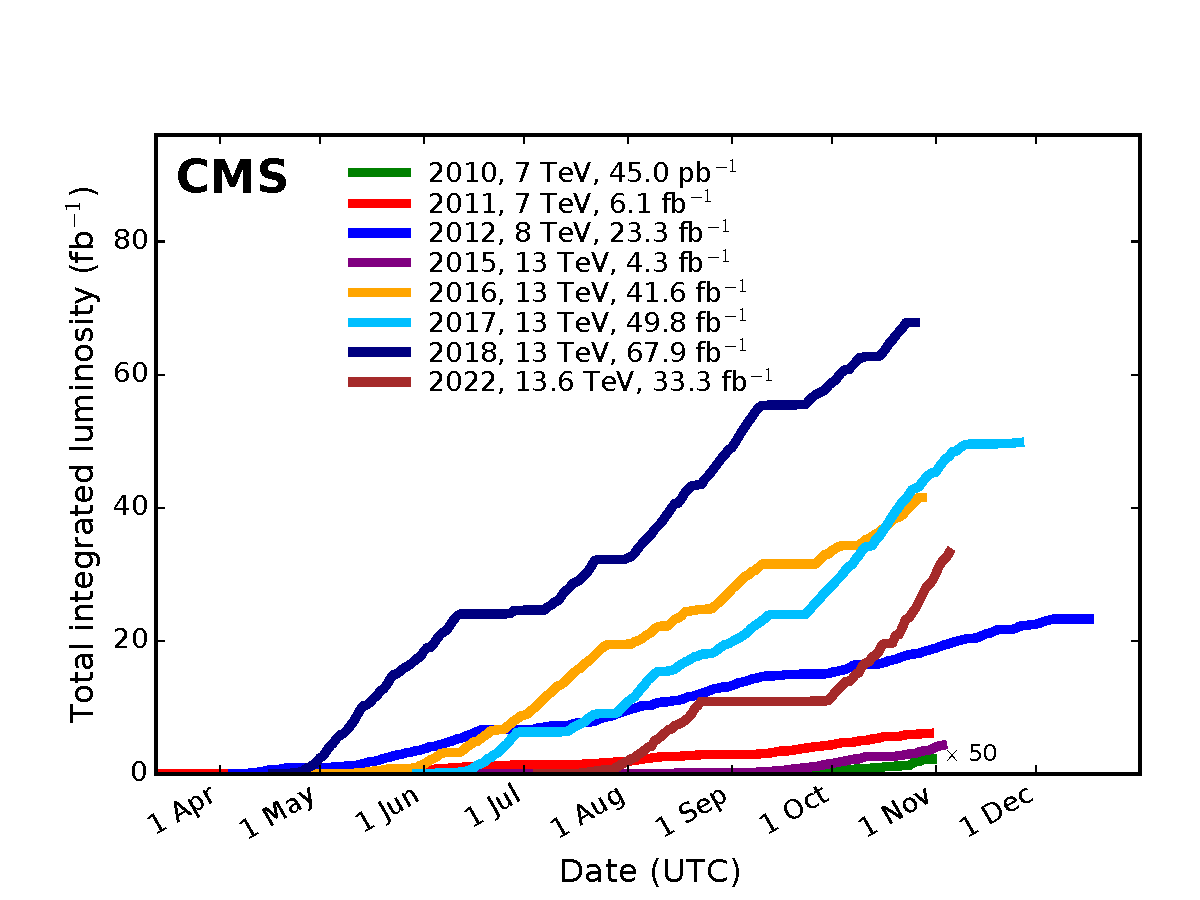
\includegraphics[width=0.34\textwidth]{figs/03_experiment/int_lumi_cumulative_pp_2.pdf}
	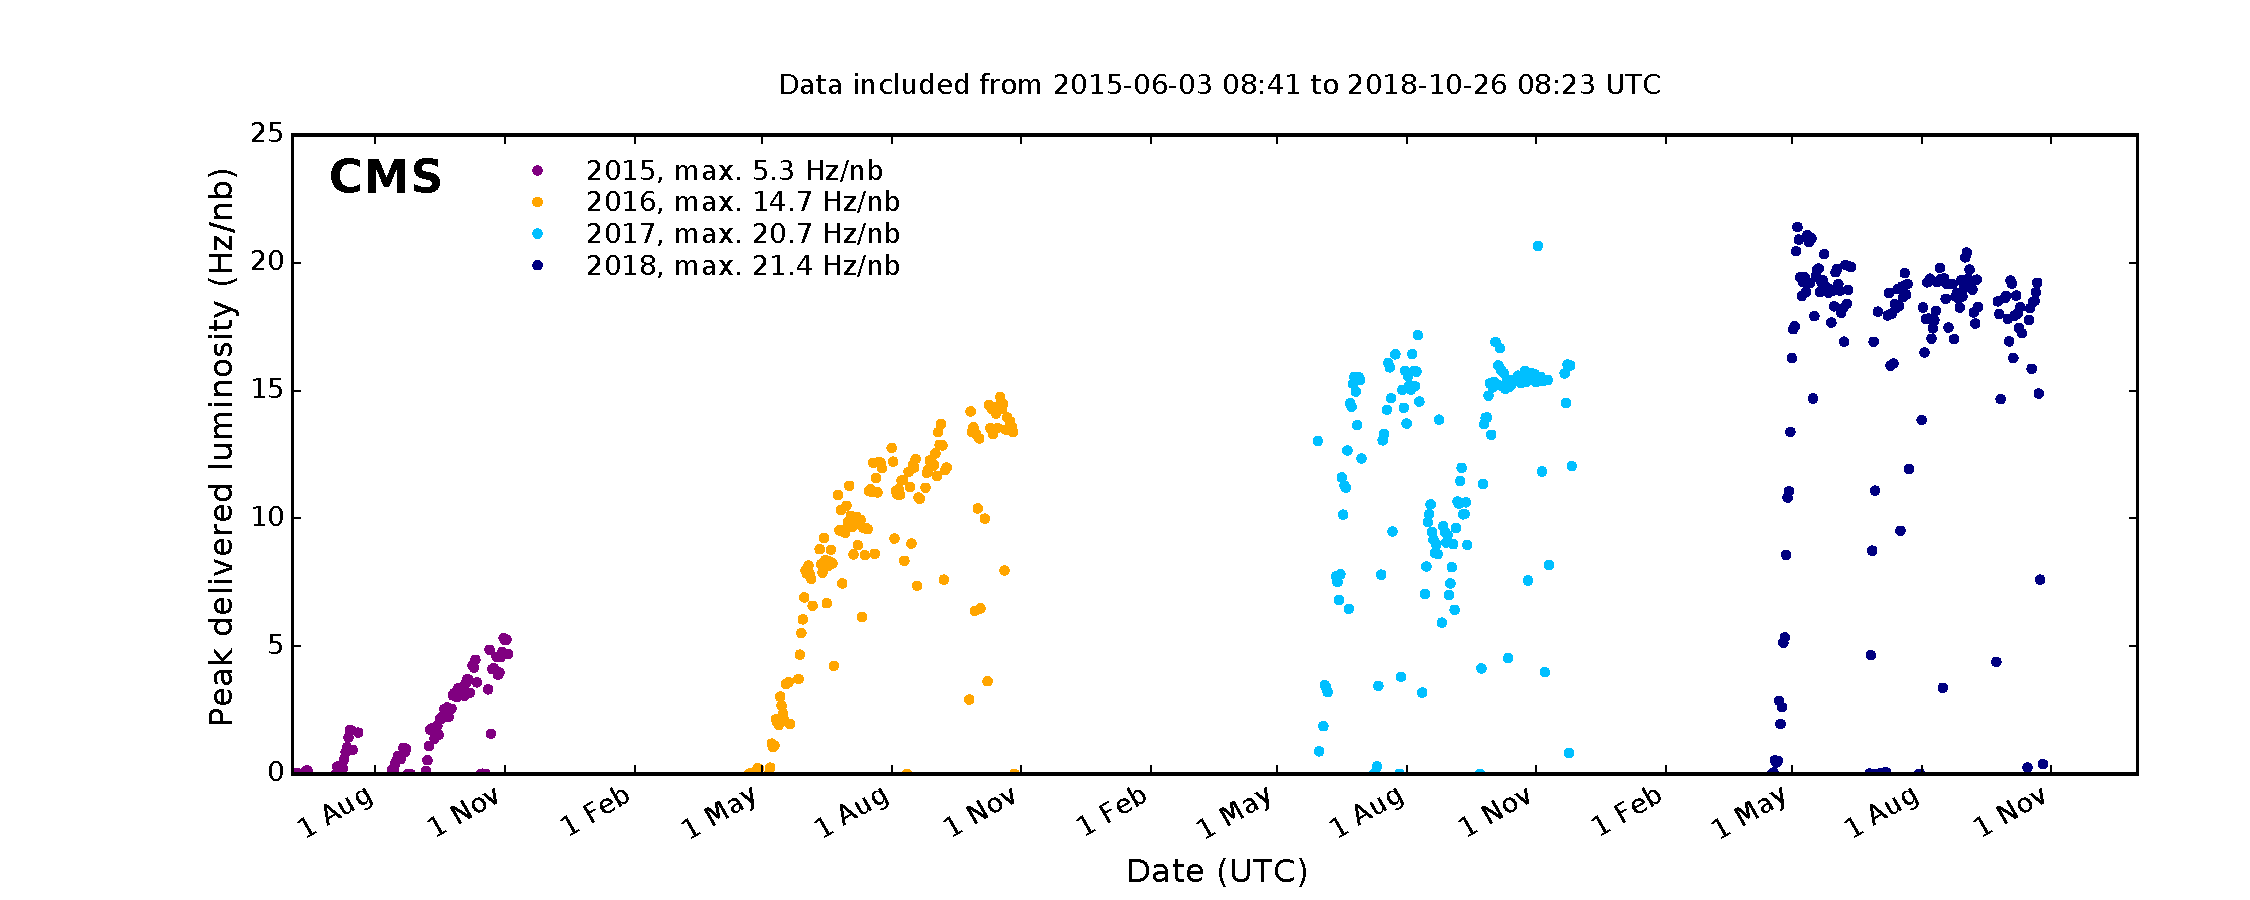
\includegraphics[width=0.65\textwidth]{figs/03_experiment/peak_lumi_pp_run2.pdf}
	\caption[LHC luminosity report. Left: breakdown of the CMS integrated luminosity by year from 2010-2022. Right:  peak luminosity from 2016-2018 data taking~\cite{CMSlumi}.]
	{LHC luminosity report. Left: breakdown of the CMS integrated luminosity by year from 2010-2022. Right: peak instantaneous luminosity from 2016-2018 data taking~\cite{CMSlumi}.}
	\label{fig:LHC_lumi}
\end{figure}

\begin{comment} % Check these numbers? pdg values do not give the correct lumi
\begin{table}[htb!]
	\caption{Description of beam parameters used to calculate the LHC luminosity, obtained from~\cite{Workman:2022ynf} and~\cite{Herr:941318}}
	\begin{center}
		\begin{tabular}{l l l}
			\hline
			Parameter & Description & Value \\
			\hline
			$N_b$ & Number of particles per bunch & $1.1\times10^{11}$\\
			$n_b$ & Number of bunches per event & $2556$\\
			$f_\mathrm{rev}$ & Revolution frequency & $11.245\unit{kHz}$\\
			$\gamma_r$ & Lorentz factor & $6929.6$\\
			$\epsilon_n$ & Transverse normalized beam emittance & $3.75\unit{\mu m\times rad}$\\
			$\beta^*$ & Amplitude function at collision point & $0.3\unit{m}$\\
			$F$ & Geometric luminosity reduction factor & 0.835\\
			\hline
		\end{tabular}
	\end{center}
\end{table}
\end{comment}

% Proton beams
The protons used in collisions are extracted from hydrogen atoms by using ionizing electric fields to strip them of their electrons. They are first accelerated to an energy of $50\unit{MeV}$ through a linear accelerator Linac2 before entering the Proton Synchrotron Booster (PSB), where they reach a kinetic energy of $1.4\unit{GeV}$. Next, the protons are accelerated by the Proton Synchrotron (PS) and Super Proton Synchrotron (SPS), where they are accelerated to $26\unit{GeV}$ and $450\unit{GeV}$ respectively. Finally, the beams are injected into the LHC where they undergo acceleration to $6.5\unit{TeV}$, producing the desired center of mass energy of $\sqrt{s}=13\unit{TeV}$.

\begin{figure}[htbp]
	\centering
	\includegraphics[width=0.825\textwidth]{figs/03_experiment/CCC-v2018-print-v2.pdf}
	\caption[Diagram of the CERN accelerator complex during 2018 data taking. Protons begin as hydrogen atoms at Linac2 and collide at various detectors along the LHC at $\sqrt{s}=13\unit{TeV}$]
	{Diagram of the CERN accelerator complex during 2018 data taking~\cite{Mobs:2636343}. Protons begin as hydrogen atoms at Linac2 and are accelerated in several stages to reach $6.5\unit{TeV}$.} 
	\label{fig:LHC}
\end{figure}

\subsection{The High-Luminosity LHC} \label{sec:HLLHC}

\section{The Compact Muon Solenoid} \label{sec:CMS}
The Compact Muon Solenoid (CMS) is one of the two general purpose detectors at the LHC, designed to reconstruct physics events from proton-proton collisions. It is a cylindrical apparatus with its major axis aligned with the proton beams from the LHC, consisting of several concentric layers of specialized detectors. The innermost layer consists of a silicon tracker, followed by an electronmagnetic and hadronic calorimeter (ECAL and HCAL, respectively). Surrounding those is the superconducting solenoid, which provides a $3.8\unit{T}$ magnetic field to  the trajectory of charged particles. Lastly, layers of muon chambers are interspaced with an iron return yolk, designed to contain the magnetic field lines near the muon chambers.

\begin{figure}[htbp]
	\centering
	\includegraphics[width=0.9\textwidth]{figs/03_experiment/cms_160312_02.pdf}
	\caption[Cutaway diagram of CMS showcasing major detector components~\cite{Sakuma:2665537}.]
			{Cutaway diagram of CMS showcasing major detector components~\cite{Sakuma:2665537}.}
	\label{fig:CMS}
\end{figure}

\subsection{CMS Coordinate System} \label{sec:CMS_coord}
The origin of the CMS coordinate system is located at the center of the detector, at the nominal collision point of the proton beams. The $+\hat{x}$ axis points radially towards the center of the LHC, while the $+\hat{y}$ axis points vertically upward. This sets the $+\hat{z}$ direction along the beamline, counterclockwise along the LHC. Due to the cylindrical symmetry of CMS, coordinates in the $\hat{x}$-$\hat{y}$ plane are commonly replaced with the radius $r$ and the azimuthal angle $\phi$, which is measured from the positive $\hat{x}$-axis. The polar angle $\theta$ is measured from the $+\hat{z}$-axis, though in practice this variable is rarely used. It is more common to define the polar angle in terms of the pseudorapidity $\eta$, which is defined as
\begin{equation}
	\eta=\frac{1}{2}\ln\left(\frac{|\mathbf{p}|+p_{z}}{|\mathbf{p}|-p_{z}}\right)=-\ln{\tan\left(\frac{\theta}{2}\right)}
\end{equation}

The motivation for using $\eta$ instead of $\theta$ stems from a fundamental property of hadron colliders: the center of mass frame for particle production rarely coincides with the lab frame. Thus, when measuring the separation between particles, it is useful to define quantities that remain invariant under Lorentz transformations in the $\hat{z}$ direction. The rapidity $y$ (not to be confused with the Cartesian coordinate $\hat{y}$) is defined as
\begin{equation}
	y=\frac{1}{2}\ln\left(\frac{E+p_{z}}{E-p_{z}}\right)
\end{equation}
It is trivial to show that differences in $y$ remain invariant under Lorentz boosts along the $\hat{z}$-axis. In the highly relativistic limit, which is valid for most particles produced at the LHC, rapidity approaches pseudorapidity as $E\approx|\mathbf{p}|$. One advantage of pseudorapidity is that $\eta$ can be calculated using only geometric quantities of the detector, whereas $y$ requires calculating both the energy and momenta of a particle, making pseudorapidity the natural choice for defining the polar angle. $\eta$ can range from $\left(-\infty, \infty\right)$, where $\eta=\pm\infty$ points directly along the $\pm\hat{z}$ axis. Higher values of $\left|\eta\right|$ are commonly referred to as "forward".

\subsection{Charged Track Momentum Resolution} \label{sec:CMS_sagitta}
The 3.8\unit{\tesla} magnet curves the trajectory of charged particles, which allows us to precisely determine their momentum. Using the geometry described in section~\ref{sec:CMS_coord}, a particle with charge $q$ and transverse momentum $p_T$ travels in a circular trajectory with radius $R$ when viewed in the $r$-$\varphi$ plane. Per the Lorentz Force Law, these can be related by $p_{T} = qBR$. In particle physics, when working with an object of elementary charge, this is commonly rewritten as
\begin{equation}
	\label{eq:pt03br}
	p_{T} = 0.3BR\unit{[GeV/c]}
\end{equation}
The track followed by a charged particle traveling over a length $L$ can be described by the sagitta $s$ shown in figure~\ref{fig:sagitta}, defined by
\begin{equation} \label{eq:sagitta}
	s=R-\sqrt{R^2-\frac{L^2}{4}}
\end{equation}

\begin{figure}[htb!]
	\centering
	\begin{tikzpicture}
		\def \R{6};
		\def \alpha{30};
		\coordinate (origin) at (0, 0);
		\coordinate (x1) at ({\R*sin(-\alpha)}, {\R*cos(\alpha)});
		\coordinate (x2) at ({\R*sin(\alpha)}, {\R*cos(\alpha)});
		\coordinate (s1) at (0, {\R*cos(\alpha)});
		\coordinate (s2) at (0, \R);
		\draw[dashed] (origin) -- node[below,left]{R} (x1);
		\draw[dashed] (origin) -- (x2);
		\draw (x1) -- node[below]{L/2}(s1);
		\draw (s1) -- (x2);
		\draw (origin) -- (s1);
		\draw (s1) -- node[left]{S} (s2);
		\draw[<-,domain={90-\alpha}:{90+\alpha}] plot ({\R*cos(\x)}, {\R*sin(\x)});
	\end{tikzpicture}
	\caption{Diagram showing the sagitta for a charged particle track}
	\label{fig:sagitta}
\end{figure}

For highly energetic particles, the length $L$ is substantially smaller than the radius $R$, so the sagitta can be approximated as
\begin{equation} \label{eq:sagitta_approx}
	s\approx\frac{L^2}{8R}=\frac{0.3BL^2}{8p_T}
\end{equation}

The relative uncertainty of the momentum is proportional to the uncertainty of the sagitta, the track length L, and the magnetic field B as
\begin{equation} \label{eq:dptOverpt}
	\frac{\delta p_T}{p_T}\propto\frac{p_T}{BL^2}\delta s
\end{equation}
Therefore, a long lever arm and high magnetic field strength are crucial to precisely determine the momentum of energetic particles.

\subsection{Inner Tracker} \label{sec:CMS_tracker}
The CMS inner tracker is the first detector surrounding the primary interaction point (IP). Its purpose is to measure the tracks from charged particles as they curve in the strong magnetic field within CMS in order to calculate their momentum and reconstruct secondary vertices. As the closest detector to the primary IP, the tracker experiences the highest particle flux within CMS, and must have high enough granularity to distinguish the multitude of tracks. This high granularity also lends the inner tracker the best momentum resolution for charged tracks out of all the subdetectors comprising CMS, with a momentum resolution of 2.8\% for a 100\unit{GeV} muon~\cite{The_CMS_Collaboration_2014}. The high flux also makes the detector susceptible to radiation damage, so the tracker must be robust in order to maintain efficiency over the long operational period of the LHC. 

The inner tracker utilizes silicon tracking modules composed of P-N type junctions to detect the location of charged particles. When an external voltage is applied to a module, particles passing through will deposit energy and create electron-hole pairs, which drift to their respective electrodes and generate an electrical signal. The applied voltage is tuned such that only a small amount of energy is required to produce electron-hole pairs, which reduces the total amount of material required in order to minimize the energy loss of the charged particles. The inner layer of the tracker is composed of higher granularity pixel detectors, while the outer layer is composed of coarser silicon strips.


\subsubsection{Silicon Pixel Detector} \label{sec:CMS_pixel}
The pixel detector is comprised of 124 million silicon pixel sensors, each with an area of $100\times150\unit{\mu m^2}$ and a thickness of $300\unit{\mu m}$. The barrel (BPIX) consists of four cylindrical layers of pixel sensors spanning from $z=-54\unit{cm}$ to $z=54\unit{cm}$ at radii of $r=2.9$, $6.8$, $10.9$, and $16\unit{cm}$. The endcap (FPIX) consists of three layers located at $z=\pm29.1$, $\pm39.6$, and $\pm51.6\unit{cm}$, which when combined with the barrel nets a total sensitive area of $1.85\unit{m^2}$ with coverage up to $\abs{\eta}<2.5$. With regards to detector performance, the pixel detector provides spatial resolution of $9.5 \unit{\mu m}$ in the $r$-$\phi$ direction and $22.2 \unit{\mu m}$ in the $z$ direction, as well as a hit efficiency of $>99\%$ in each layer at nominal LHC luminosity, with the innermost BPIX layer dropping to $97.5\%$ at peak run 2 efficiency~\cite{CMSPixelP1}.

\begin{figure}[htbp]
	\centering
	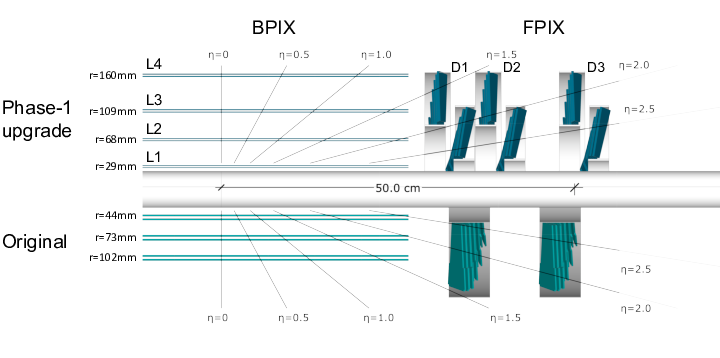
\includegraphics[width=0.85\textwidth]{figs/03_experiment/20120828_01_pixel_phase1_largesharp.png}
	\caption
	[$r$-$z$ slice of the CMS pixel detector~\cite{CMSPixelP1}]
	{$r$-$z$ slice of the CMS pixel detector comparing original design (bottom, teal) with the Phase-I upgrade implemented in 2016/17, which added one layer to both the FPIX and BPIX (top, blue)~\cite{CMSPixelP1}.}
	\label{fig:pixel}
\end{figure}

\subsubsection{Silicon Strip Detector} \label{sec:CMS_strip}
The silicon strip detector surrounds the pixel detector, and is segmented into a tracker inner barrel (TIB), tracker outer barrel (TOB), tracker inner disks (TID), and tracker endcap (TEC). The TIB consists of four layers covering $\left|z\right|<65\unit{cm}$ and radius $25.5\unit{cm}<r<49.8\unit{cm}$. The endcaps of the TIB are covered by the TID, consisting of three disks covering $90<\left|z\right|<90\unit{cm}$. Surrounding the TIB is the TOB, with six layers spanning $\left|z\right|<188\unit{cm}$ and $60.8<\left|r\right|<108\unit{cm}$. Lastly, both the TOB and TID are closed by the TEC, which covers radii ranging from $22<r<113.5\unit{cm}$ and stretches from $124<\left|z\right|<280\unit{cm}$.

The strip detector modules function similarly to the pixel modules, but utilize much larger silicon strips due to the expected reduced particle flux compared to the pixel detector. Each strip detector is composed of $300\unit{\mu m}$ thick micro-strip sensors with pitch varying from $80-205\unit{\mu m}$ to form $7-12.5\unit{cm}$ long strip modules. Overall, the strip detector uses 15,148 modules covering an area of $200\unit{m^2}$ up to $\left|\eta\right|<2.5$.

\begin{figure}[htbp]
	\centering
	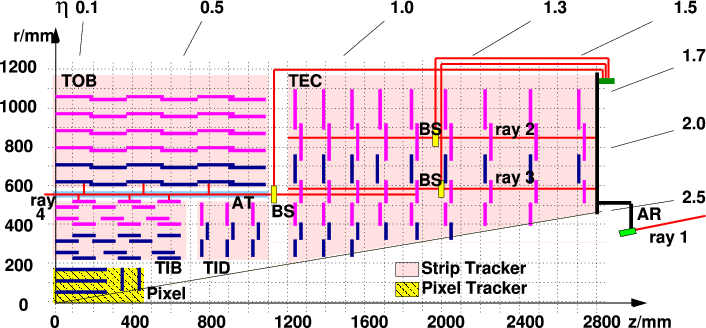
\includegraphics[width=0.85\textwidth]{figs/03_experiment/las.png}
	\caption
	[$r$-$z$ slice of the CMS silicon detector, detailing the four main components of the strip detector~\cite{Chatrchyan:1211825}]
	{$r$-$z$ slice of the CMS silicon detector, detailing the four main components (TIB, TOB, TID, and TEC) of the strip detector. Pixel detector is shown in its Run-I configuration~\cite{Chatrchyan:1211825}.}
	\label{fig:strip}
\end{figure}

\subsection{Electromagnetic Calorimeter} \label{sec:CMS_ECAL}
The CMS Electromagnetic Calorimeter (ECAL) is designed to stop and capture the energy of photons and electrons. When a high energy photon or election enters the ECAL, it primarily interacts with the material in the detector through $e^+e^-$ pair production or bremsstrahlung, respectively. These processes create more photons and electrons that result in an electromagnetic cascade until the particles lose enough energy that ionization and compton scattering processes begin to dominate. This process is known as an electromagnetic shower. The light from these showers is measured using photodetectors to determine the initial energy of the incident particle with resolution given by

\begin{equation}
	\left(\frac{\sigma_E}{E}\right)^2=\left(\frac{2.8\%}{\sqrt{E/\mathrm{GeV}}}\right)^2+\left(\frac{12\%}{E/\mathrm{GeV}}\right)^2+(0.3\%)^2
\end{equation}
The first term arises from statistical fluctuations in the electromagnetic shower and light production, which is a poisson process and therefore proportional to $1/\sqrt{\mathrm{E}}$. The second term is due to the noise in the detector electronics. The last constant term is due to imperfecions in the detector such as non-uniformity, radiation damage, and calibration uncertainty.
The material used for an electromagnetic calorimeter can be characterized by the radiation length ($X_0$) and moli\`ere radius ($R_M$). The radiation length is the average distance an electron will travel before its energy is reduced by a factor of $1/e$, and is roughly proportional to $A/Z^2$, where A is the atomic mass and Z is the atomic number. The moli\`ere radius is directly proportional to the radiation length and measures the spread of an electromagnetic shower in the transverse direction. Both are generally measured in units of $\left[\si{g}\unit{cm^{-2}}\right]$, but can be divided by the density of the material to obtain a distance in $\left[\si{cm}\right]$. A low radiation length and Moli\`ere radius ensure all of the energy is captured in the detector and is contained to a small area to precisely determine the position of an incident particle. It is for this reason that the ECAL is composed of lead-tungstate (PbWO$_4$): a dense, high Z scintillator crystal with $X_0=7.39\unit{g/cm^2}$ (or $0.89\unit{cm}$ after dividing by the density of PbWO$_4$) and $R_M=2.2\unit{cm}$~\cite{Workman:2022ynf}.

The ECAL is constructed from 61200 + 15000 lead-tungstate crystals in the barrel + endcap region. Barrel crystals have a cross sectional area of $2.2\times2.2\unit{cm^2}$ to match the moli\`ere radius and a depth of 23$\unit{cm}$ (or $25.8\,X_0$), and are arranged in rings along the $\phi$ direction, tilted to align with lines of constant $\eta$. The barrel has an inner radius of $129\unit{cm}$ and covers an eta region up to $\left|\eta\right|<1.479$. Endcap crystals have a slightly higher cross sectional area of $2.6\times2.6\unit{cm^2}$ and a slightly lower depth of 22$\unit{cm}$, and are arranged in an $x$-$y$ grid. The endcap provides the remaining coverage from $1.479<\left|\eta\right|<3.0$. A diagram showing the geometry of the ECAL can be seen in figure~\ref{fig:ecal}. The size and alignment of the crystals is designed to contain showers from incident photons/electrons within a $2\times2$ grid of crystals.

One common process in CMS is the production of $\pi^0$s, which decay to two photons. When the two photons deposit their energy into the ECAL, they can fake a signal from a single high energy photon. In the barrel, the two photons are generally separated by $\sim1\unit{cm}$, so the crystal granularity can be used to distinguish this background from real, high energy photons. However, $\pi^0$s in the forward region tend to be higher energy (commonly referred to as "more boosted"), resulting in separations on the order of millimeters. In order to identify these background events, a higher granularity detector known as a preshower is placed before the ECAL endcap. It consists of a layer of lead absorber to initiate the shower, followed by silicon strip sensors to measure the tracks within the shower. The lead has a thickness of $1.57\unit{cm}$ (or $2.8X_0$), which is thick enough to reliably cause a shower while only causing energy loss of a few percent before the shower can reach the ECAL. The silicon strips are similar to those in the inner tracker, with a pitch of $1.9\unit{mm}$~\cite{TOURNEFIER2001355}.

\begin{figure}[htpb]
	\centering
	\includegraphics[width=0.85\textwidth]{figs/03_experiment/cms_ecal.pdf}
	\caption
	[Geometry of the CMS ECAL showing the barrel, endcap, and preshower, adapted from~\cite{Marzocchi2019}]
	{Geometry of the CMS ECAL showing the barrel, endcap, and preshower, adapted from~\cite{Marzocchi2019}.}
	\label{fig:ecal}
\end{figure}


\subsection{Hadronic Calorimeter} \label{sec:CMS_HCAL}
The CMS Hadronic Calorimeter (HCAL) is a sampling calorimeter surrounding the ECAL. Unlike the ECAL, which is a homogeneous calorimeter where the crystals both induce showers and scintillate, the HCAL is composed of alternating layers of dense absorber and scintillator. The absorber induces hadronic showers - cascades of hadrons resulting from inelastic scattering off a target nuclei. Particles in hadronic showers then pass through the scintillator, which produces light that gets transmitted through wavelength shifting fibers and read out by photodetectors, before repeating this process with the next layer of absorber/scintillator. The measured energy can be summed in sequential layers of detectors (referred to as "towers") to calculate the total energy of the incident hadron. As an additional complication, several hadrons decay to electrons or photons, which will create electromagnetic showers, requiring the scintillator to have good response to electromagnetic interactions. The HCAL must be hermetic, as a complete picture of the energy from proton collisions is required to infer the production of particles like neutrinos, which are otherwise invisible to the detector.

The relevant property for a hadronic absorber is the nuclear interaction length $\lambda_I$, which is the mean distance a hadron will travel before undergoing an inelastic nuclear interaction. Like the radiation length, $\lambda_I$ is measured in $\left[\unit{g}\unit{cm^{-2}}\right]$ and can be divided by the density to obtain a distance in $\left[\unit{cm}\right]$. It is proportional to the density of nuclear matter, which goes as $\text{A}^{1/3}$. The HCAL uses a combination of brass and stainless steel, both of which have an interaction length of $\sim16.5\unit{cm}$~\cite{Baiatian:1049915}.

The HCAL consists of four subsystems: an inner barrel (HB), an outer barrel (HO), an endcap (HE), and a forward calorimeter (HF). The HB covers $\left|\eta\right|<1.3$ with 36 azimuthal wedges, each containing 17 layers of alternating brass absorber and scintillator. These wedges begin at a radius of $1.806\unit{m}$ and are $89\unit{cm}$ thick, resulting in a minimum of $5.3\,\lambda$ at $\eta=0$, increasing to $10\,\lambda$ and $\eta=1.2$. The HE consists of two disks, also formed of 36 wedges with 19 layers of brass absorber and scintillator, totaling 10 $\lambda_I$ in order to contain highly boosted, forward jets. The HE extends the coverage of the HCAL up to $\left|\eta\right| < 3.0$. The HO is located outside the magnetic coil to catch high energy ($>100\unit{GeV}$) hadrons that escape the HB. It consists of five rings in eta, covering up to $\left|\eta\right|<1.2$, and relies on the iron solenoid to induce hadronic showers. The HF covers the most forward region of $3<\left|\eta\right|<5$. This zone has the highest exposure of radiation, and so the detector must be sensitive only to the highest energy particles and robust against damage from heavy radiation. It uses steel as the absorber and quartz fibers to scintillate through Cherenkov radiation. The four subsystems provides a minimum of $10\,\lambda$ to capture incident hadrons.

\begin{figure}[htpb]
	\centering
	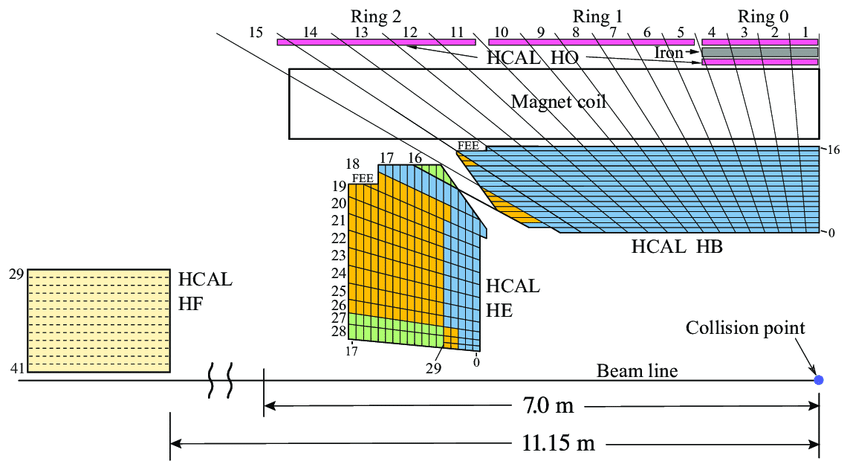
\includegraphics[width=0.85\textwidth]{figs/03_experiment/A-schematic-view-of-one-quarter-of-the-CMS-HCAL-during-2016-LHC-operation-showing-the.png}
	\caption
	[$r$-$z$ slice of the CMS HCAL showing the HB, HE, HF, and HO~\cite{Sirunyan:2691403}]
	{$r$-$z$ slice of the CMS HCAL showing the HB, HE, HF, and HO~\cite{Sirunyan:2691403}.}
	\label{fig:hcal}
\end{figure}

\subsection{Muon Detectors} \label{sec:CMS_Muons}
The muon chambers lie outside the magnetic solenoid as the outermost subsystem in CMS. Due to the distance and amount of material between them and the primary IP, they are the lowest occupancy detectors, with few particles other than muons able to reach them before decaying or stopping in the inner subsystems. Although they lie outside the solenoid, the iron yolk pulls the magnetic field back to curve the trajectory of muons, which is required calculate their momenta. The detector subsystem is composed of three types of gaseous detection chambers: drift tubes (DTs), resistive plate chambers (RPCs), and cathode strip chambers (CSCs). A diagram showing the configuration of these detection chambers can be seen in figure~\ref{fig:Muons}.

The operating physics principles of all three chambers are similar: muons pass through a gas mixture and ionize the gas, knocking loose electrons. Anodes and cathodes create an electric field inside the gas chamber, causing the electrons to drift to the anode where they can be measured and read out by electronics. Electrons that are excited but not ionized from the incident muon will emit photons as they transition back to a lower energy level, thus a quenching gas is used to absorb these photons to prevent further cascades. The specifics of the three detectors are described in sections~\ref{sec:CMS_DT}-\ref{sec:CMS_RPC}.

\begin{figure}[htpb]
	\centering
	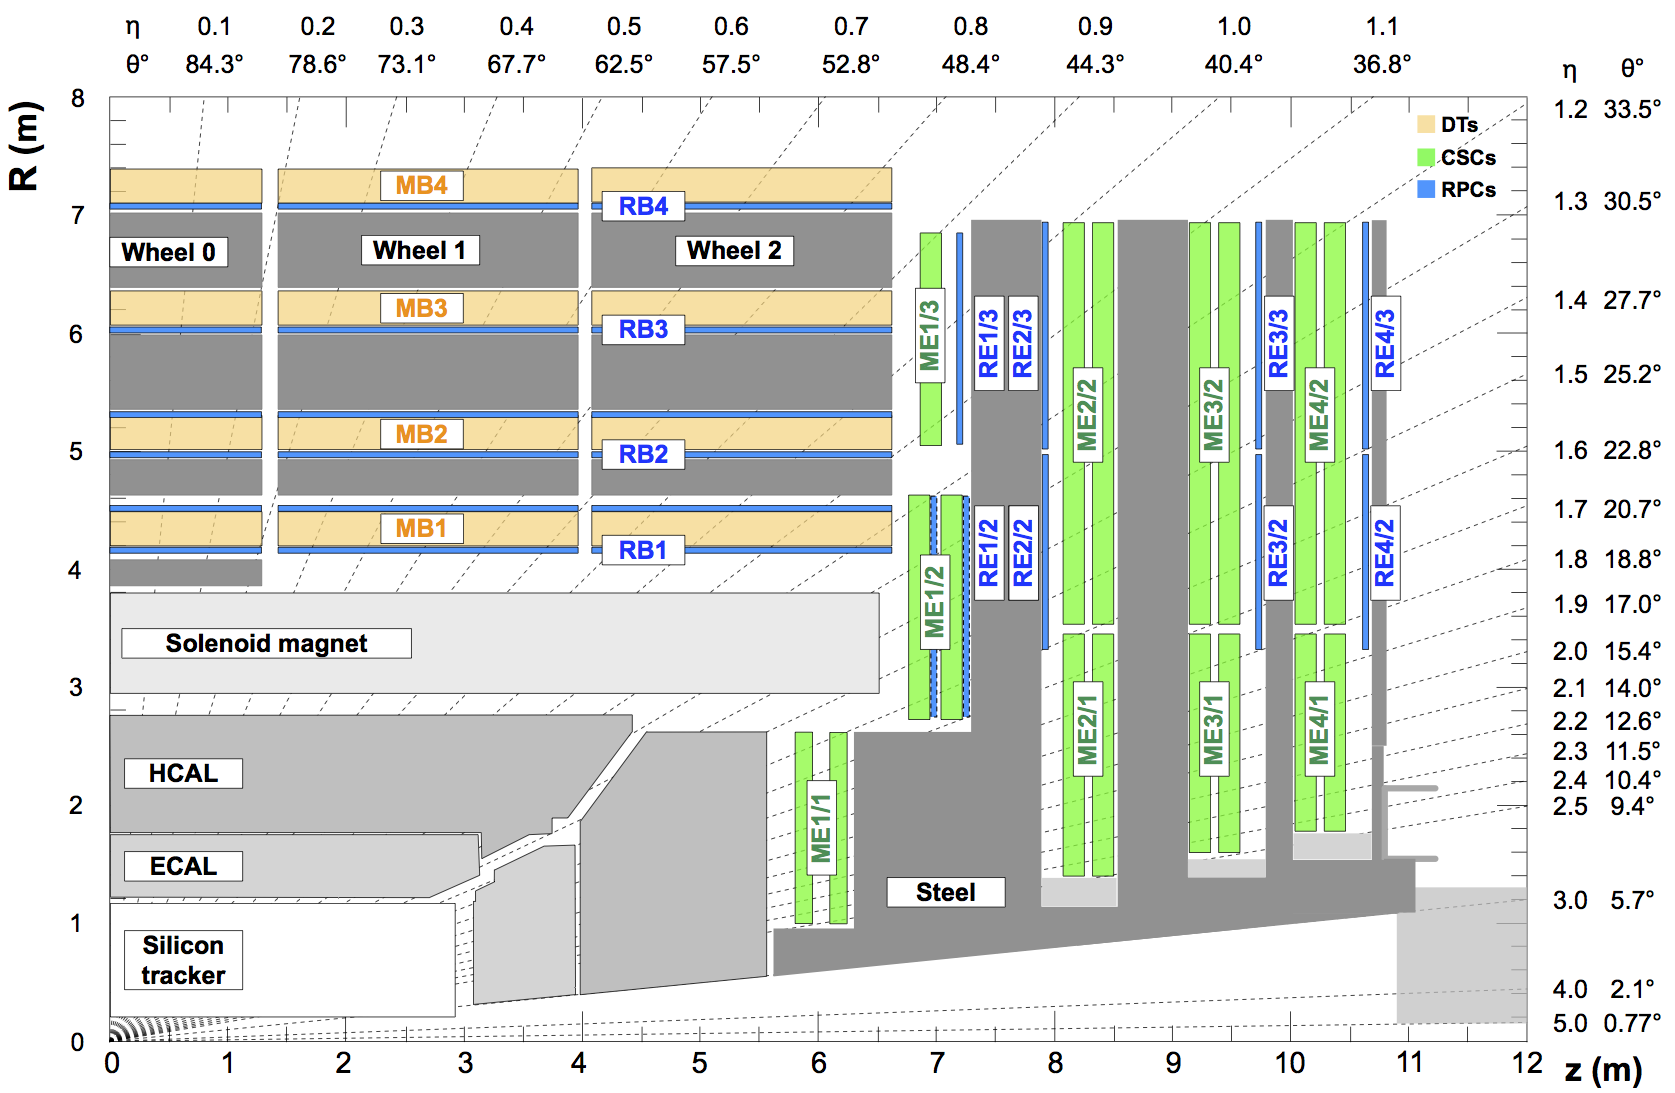
\includegraphics[width=0.85\textwidth]{figs/03_experiment/Muon_system.png}
	\caption
	[Diagram of the CMS Muon system~\cite{Sirunyan:2313130}]
	{$r$-$z$ cross section of the CMS muon detector subsystem, configured for the 2016-2018 data taking run. The barrel consists of five wheels of DTs and RPCs in $\eta$, each wheel consisting of four layers in $r$ and 12 sectors in $\phi$, covering up to $\left|\eta\right| < 1.2$. The endcap consists of four layers of DTs and RPCs in $z$~\cite{Sirunyan:2313130}.}
	\label{fig:Muons}
\end{figure}

\subsubsection{Drift Tubes} \label{sec:CMS_DT}
Drift tubes are used in the barrel of the muon system, covering $\left|\eta\right| < 1.2$. They consist of long chambers filled with an mixture of Ar/$\text{CO}_2$, with an anode wire running lengthwise through the center and cathode strips along the edges. Electrode strips along the outer edge of the chamber shape the electric field lines to linearize the drift velocity of electrons throughout the chamber. When a muon passes through the chamber, ionized electrons follow the electric field lines towards the anode wire. Due to the known field inside the chamber, the drift time can be used to calculate the transverse distance from the wire to the incident muon with a resolution of $250\unit{\mu\m}$. The DTs are arranged in superlayers, which consist of 4 layers of DTs, with subsequent superlayers alternating in the $r$-$z$ and $r$-$\phi$ direction in order to obtain the muon trajectory/curvature in both the $\eta$ and $\phi$ direction. Figure~\ref{fig:DT} shows a diagram of a DT superlayer and a single DT cell.

\begin{figure}[htpb]
	\centering
	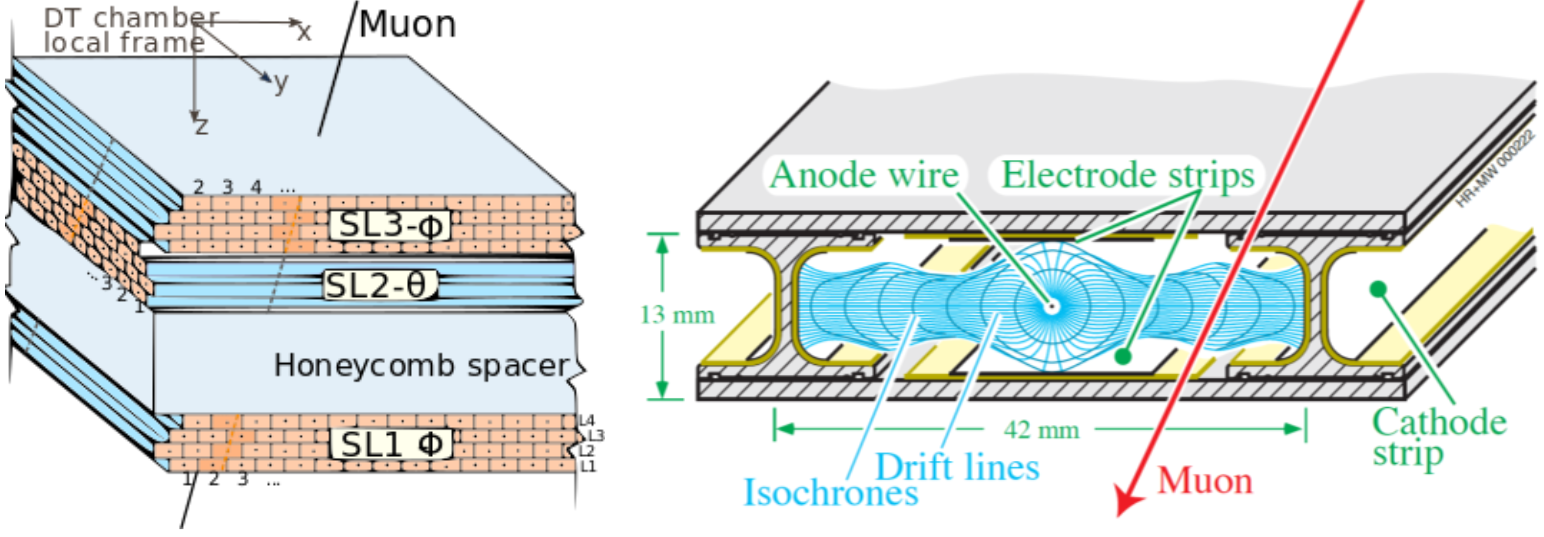
\includegraphics[width=0.85\textwidth]{figs/03_experiment/CMS_DT.png}
	\caption
	[Diagram of the CMS Drift Tubes~\cite{CMSDT}]
	{Drift tube superlayers are aligned in alternating orientations in order to provide a complete picture of muon trajectories (left). A cross section of a single drift tube chamber (right). Electrons ionized from the muon drift to the anode wire to produce a measurable current~\cite{CMSDT}.}
	\label{fig:DT}
\end{figure}

\subsubsection{Cathode Strip Chambers} \label{sec:CMS_CSC}
Cathode strip chambers are used in the endcaps of the muon system to provide coverage from $0.9<\left|\eta\right|<2.4$. CSC modules are trapezoidal chambers filled with a mixture of Ar/$\text{CO}_2$/$\text{CF}_4$ and arranged in disks to cover the muon endcap. Each module is composed of six layers of radial cathode strips, which have high granularity in $\phi$, and transverse anode wires which provide granularity in $r$. Similar to the DTs, muons passing through CSC chambers ionize the gas molecules, knocking loose electrons which drift to the anode wires. The charge from these electrons can is measured and provides the position of the muon in $r$. Simultaneously, the electrons induce a charge in the cathode strips, which provides the position of the muon in $\phi$. One chamber provides a spatial resolution of between $40-50\unit{\mu m}$ with a time resolution of $3\unit{ns}$.

\begin{figure}[htpb]
	\centering
	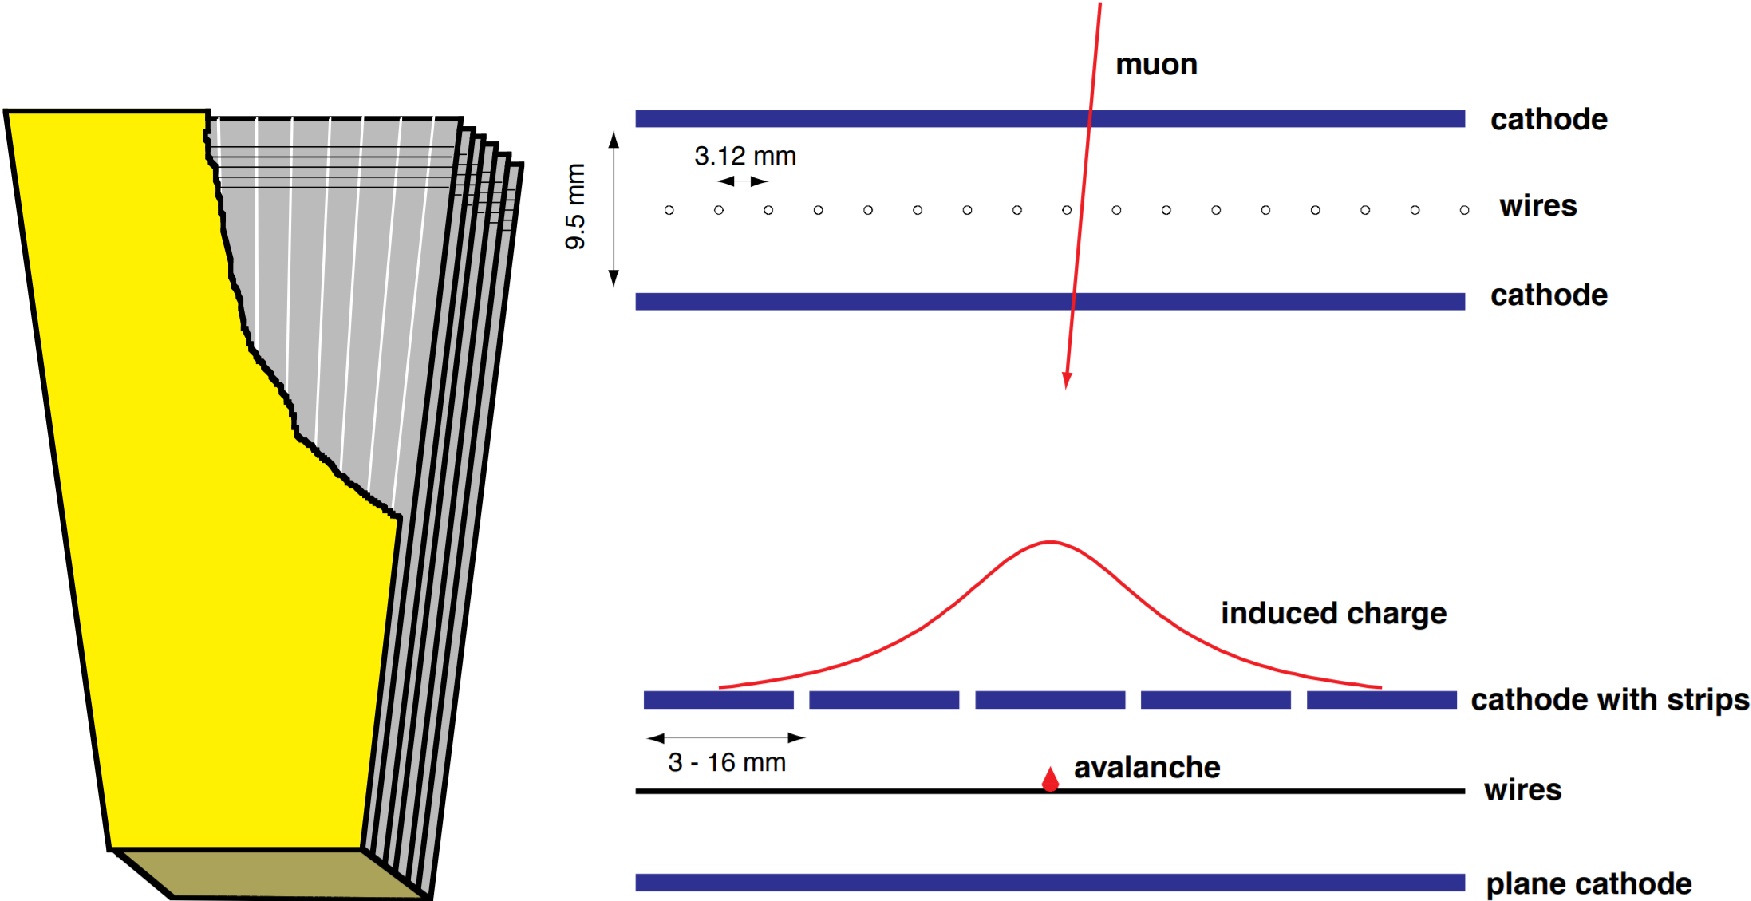
\includegraphics[width=0.85\textwidth]{figs/03_experiment/cms_csc.pdf}
	\caption
	[Cut-away diagram of a single CSC module~\cite{DeBruyn:2797803}]
	{Cut-away diagram of a single CSC module showing the six layers of radial cathode strips and transverse anode wires (left). Muons ionize the gas chamber, causing an avalanche of electrons on the anode wires and inducing a charge on the cathode strips (right)~\cite{DeBruyn:2797803}.}
	\label{fig:CSC}
\end{figure}

\subsubsection{Resistive Plate Chambers} \label{sec:CMS_RPC}
RPC detectors are used in conjunction with the DTs and CSCs in both the barrel and endcap. One RCP consists of two high resistivity plastic plates: one positively charged anode and a negatively charged cathode which create a strong, uniform electric feel between the two. The space between the two plates is filled with a mixture of 95\% C$_2$H$_2$F$_4$ and 5\% iso-C$_4$H$_10$. Incident muons ionize the gas between the two plates, which cause a cascade of electrons towards the anode plate due to the strong electric field. External metal strips lie outside the anode in order to measure the avalanche of electrons. The coarse nature of the strips means the RPC spatial resolution is lower than that of the CSCs and DTs at around $1\unit{cm}$, but the time resolution is much faster on the order of $1\unit{ns}$. For this reason they are used to supplement the CSC and DTs to aid with triggering and accurate timing.

\begin{figure}[htpb]
	\centering
	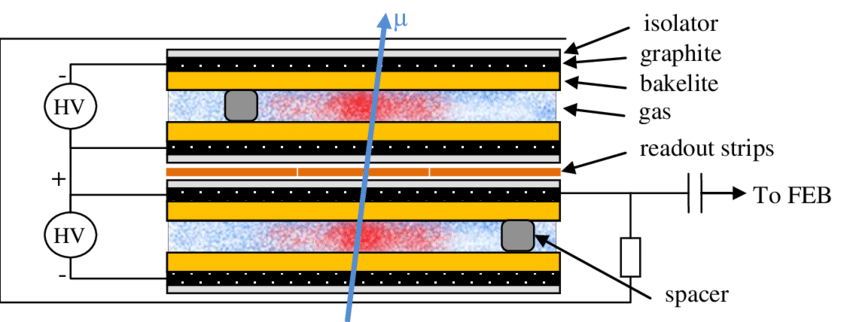
\includegraphics[width=0.85\textwidth]{figs/03_experiment/Design1.png}
	\caption
	[Diagram of the double RPC at CMS~\cite{CMSRPC_HLLHC}]
	{Diagram of the double RPC at CMS. Incident muons ionize the gas, causing a cascade of electrons towards the readout strips~\cite{CMSRPC_HLLHC}.}
	\label{fig:RPC}
\end{figure}

\subsection{Trigger System} \label{sec:CMS_trig}
The high luminosity of the LHC yields an incredibly high rate of information to store from the various detectors. Each event contains approximately $1\unit{MB}$ of data to store, which would take bandwidth and storage space beyond current capacities to save given the $40\unit{MHz}$ collision rate. Additionally, many events are soft collisions that do not contain interesting physics worth storing for further analysis. In order to reduce the rate of events and filter uninteresting collisions, CMS employs a two level trigger system. The first level is known as the Level-1 (L1) trigger and uses hardware to identify physics objects in real time. The second is known as the High-Level trigger (HLT), consisting of a conventional CPU farm which performs more advanced calculations.

\subsubsection{Level-1 Trigger} \label{sec:CMS_L1T}
The L1 trigger utilizes special processors such as Field Programmable Gate Arrays (FPGAs) in order to process coarse information from the calorimeters and muon chambers in real time. The coarse detector information, known as trigger primitives, is subjected to several algorithms to create physics objects (e.g. muons, electrons, etc). Objects passing a predetermined set of criteria are called trigger "seeds", with events that satisfy at least one seed getting passed to the HLT. A diagram of the L1 trigger architecture can be seen in figure~\ref{fig:L1T}. This entire decision making process must take place in $3.2\unit{\mu s}$ after a bunch crossing. As this is greater than the time between bunch crossings, the L1 trigger must be pipelined in order to operate continuously, while the full data is kept in a rolling buffer and read out only if the event passes a trigger seed. The L1 trigger was designed to accept events at a maximum rate of about $100\unit{kHz}$, meaning only one in every four hundred events is passed to the HLT.

\begin{figure}[htpb]
	\centering
	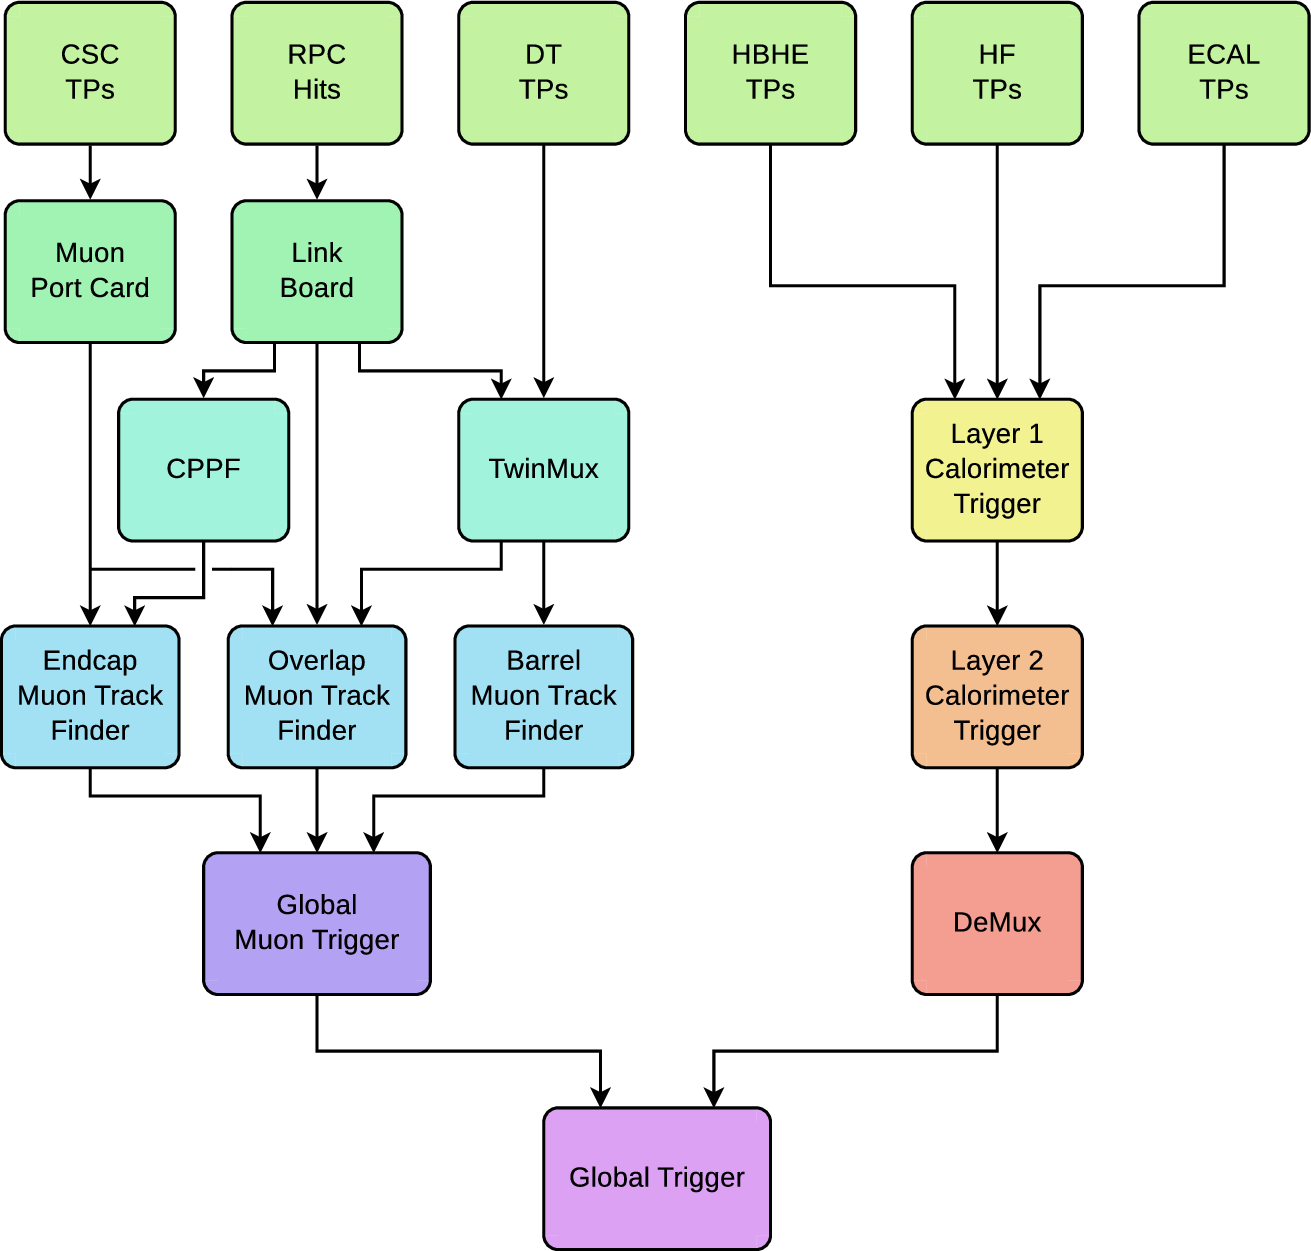
\includegraphics[width=0.85\textwidth]{figs/03_experiment/cms_l1t.png}
	\caption[CMS Level-1 Trigger architecture during Run 2~\cite{Sirunyan:2721198}]
	{Block diagram of the CMS Level-1 Trigger architecture during Run 2~\cite{Sirunyan:2721198}. Muon objects found in the barrel, overlap, and endcap regions are ranked and sorted using their momentum and quality criteria before being passed to the Global Muon Trigger (GMT), which cleans duplicate tracks and selects the top eight muons. The muons are then passed to the global trigger, which combines the muons with objects created from the calorimeters and makes the final decision to pass the event to the HLT.}
	\label{fig:L1T}
\end{figure}

\subsubsection{High Level Trigger} \label{sec:CMS_HLT}
The HLT receives the full precision detector data for events passing the L1 trigger, and is designed to reduce the final event rate to approximately $100\unit{Hz}$, five orders of magnitude less than the LHC bunch crossing rate. Information from the tracker allows the HLT algorithms to reconstruct a more complete picture of an event, as tracker information can be matched to both calorimeter hits and muon tracks to provide more detail to reconstructed physics objects. As with the L1 trigger, the HLT processes data through a series of trigger paths, which sequentially reconstruct and filter physics objects. In order to optimize computation time, the HLT uses L1 trigger seed to inform which trigger paths to use, and structures the paths in order of increasing complexity. For example, electrons are first created using only calorimeter data, then matched using coarse hits in the tracker, before being reconstructed using full tracker information. Events passing the HLT are then recorded permanently for offline reconstruction and analysis. 

\subsection{Event Reconstruction} \label{sec:CMS_Reco}
Events that pass the HLT then undergo a complete event reconstruction, where data from all sub-detectors is combined to identify each physics object created in a collision. This section provides an description of the relevant objects for this dissertation, namely muons, electrons, and photons, as well as a brief description of the particle flow (PF) algorithm used for global event reconstruction.

\subsubsection{Particle Flow} \label{sec:CMS_PF}
The global reconstruction algorithm, known as particle flow (PF), takes advantage of the unique signatures of various physics objects as they pass through each detector. Raw detector information from each subsystem is used to create building blocks of tracks and calorimeter clusters, which are then pieced together to identify individual particles and create a global event reconstruction.

Tracks are built using a Kalman Filter algorithm to fit particle trajectories to hits in the pixel and strip detectors. This process begins with a track seed which is built from hits in the pixel detector compatible with a charged particle track. The initial seed track is propagated outward to collect nearby hits in successive layers of the tracker. Once the seed and hits are collected, the track is iteratively fit to determine the final properties of the charged particle, namely the origin, $\pt$, and direction. Various quality cuts are applied based on the number of hits in order to reject fake or misidentified tracks.

Clusters are seeded from individual cells in the calorimeters with an energy above a preset threshold. Adjacent cells are added to the cluster if they have an energy above twice the expected noise level to form superclusters. The average noise level per cell in the electromagnetic calorimeter is roughly 40 and 150 MeV in the barrel and endcap respectively, while the noise per tower in the hadronic calorimeter is around 200 MeV~\cite{Sirunyan:PF}. Lastly, various algorithms calculate the substructure of these topological clusters to separate contributions from individual sources into smaller clusters.

Tracker tracks, muon tracks, and calorimeter clusters then form "pf blocks" in a process known as linking, where topologically associated objects from one or more subdetector are linked. The particle flow algorithm then takes these blocks and reconstructs the individual particles. In order, the algorithm reconstructs muons, electrons and isolated photons, charged hadrons, and neutral particles. After each step the corresponding tracks and clusters are removed from the pf blocks to prevent double counting. Once all objects are reconstructed, a final post processing step is done to further reduce mis-reconstructed particles.

\subsubsection{Muon Reconstruction} \label{sec:CMS_Reco_mu}
Muon reconstruction relies on tracks reconstructed in the inner tracker (tracker tracks) and tracks reconstructed in the muon systems. There are three categories of muon objects based on the method used to reconstruct tracks.

\textit{Standalone-muon tracks} utilize a Kalman-filter algorithm to construct tracks using only information from the muon system. Tracks seeds are formed from CSC or DT track segments and propagated to nearby hits in the muon chambers.

\textit{Global muon tracks} begin with a standalone track, which is propagated to the silicon tracker and matched to compatible tracker tracks. Two tracks are matched if the standalone track and tracker track can be propagated to a common surface. The track is then refit using a Kalman filter by combining the information from the tracker and standalone track. 

\textit{Tracker muon tracks} recapture muons in detector gaps and lower p$_T$ muons that leave hits in the muon chambers but do not fully penetrate the muon system. In these cases, it is common for a muon to leave a segment of hits in consecutive DT/CSC layers that are compatible with a track but not produce a standalone track. Tracker muons are formed by propagating all tracker tracks with p$_T > 0.5\unit{GeV}$ and p $>2.5\unit{GeV}$ into the muon chambers, and matching to nearby muon segments.

This reconstruction has an efficiency of 99\% for muons produced within the geometric acceptance of the muon system\cite{Sirunyan:2313130}. Muon objects are then fed into the PF algorithm, which performs selection criteria based on the quality of the track. As the purity of each track varies based on type (e.g. hadrons that "punch through" the HCAL are more probable to be reconstructed as track muon tracks), the cuts vary for each category.

\subsubsection{Electron/Photon Reconstruction} \label{sec:CMS_reco_egamma}
In theory, electrons should leave a smoothly curving track in the silicon tracker and deposit nearly all of their energy within a few crystals in the ECAL. However in practice, electrons frequently interact with the material in the tracker, which induces electromagnetic showers before the particle can reach the calorimeter, resulting in tracks which can have sudden changes in curvature and ECAL clusters that are smeared in $\varphi$.

The PF algorithm accounts for these factors when track fitting and forming clusters for electrons. Electron track seeds are formed when the momentum of a track and the energy of a linked ECAL cluster are compatible with unity~\cite{Sirunyan:PF}. These tracks are refit using a Gaussian Sum Filter (GSF), which uses a sum of gaussian distributions to approximate the probability density function for energy loss due to bremsstrahlung~\cite{Adam_2005}.

Bremsstrahlung photons are emitted tangent to the trajectory of the electron, which bends in $\varphi$. To ensure this energy is accounted for in the reconstruction, clusters located tangent to the GSF track are linked in the same PF block to the track and supercluster. Additionally, the total cluster energy is calibrated as a function of energy and $\eta$ to account for energy loss. Photons, which are seeded by ECAL clusters with no linked GSF track, can undergo the same process of pair production to induce electromagnetic showers. As such, photon candidate clusters are subject to the same energy calibration.

Several cuts are applied to the candidate particles to reject background from hadronic processes. Electrons and photons are expected to have a low ratio of linked HCAL cluster energy to their ECAL cluster energy. Electron tracks have several variables that are fed to a boosted decision tree, which decides whether or not to accept an electron candidate. As described previously, all tracks and clusters used to reconstruct electrons and photons are then removed from the PF blocks used to reconstruct additional particles.
% !TEX = root../thesis.tex

\chapter{Real Time Muon Reconstruction at the Compact Muon Solenoid}
\label{chap:kbmtf}

\section{Introduction} \label{sec:kbmtf_intro}
Section~\ref{sec:CMS_L1T} provides an overview of the L1 trigger and its importance to the CMS trigger system. This section will detail the design and performance of a Kalman Filter algorithm used in the L1 trigger to identify muon tracks in the barrel region ($|\eta|<0.83$) of the CMS detector. This algorithm, known as the Kalman Barrel Muon Track Finder (KBMTF), was fully implemented for 2018 data taking and received improvements for continued use in Run-3.

The L1 barrel muon trigger receives inputs from the TwinMux system, which creates trigger primitives by combining information from the DT and RPC detectors to determine the position, trajectory, and timing of hits from incident muons at each station~\cite{Triossi_2017}. These hits, referred to as ``stubs'', are fed to the L1 barrel muon trigger electronics where they are used to reconstruct muon tracks which are delivered to the Global Muon Trigger. The previous track finding algorithm, known as the Phase-I Barrel Muon Track Finder (BMTF), used a maximum of two stubs to reconstruct muon trajectories and was designed under the assumption that muons originate only from the beam line. As a part the L1 Trigger upgrade, the KBMTF algorithm was developed to improve on the BMTF in two key areas: improving performance on prompt muons by utilizing stubs from all four stations and gaining the capability to reconstruct tracks from displaced muons.

\section{The Kalman Filter Algorithm} \label{sec:kalman_filter}
A Kalman Filter is a tracking algorithm that performs a recursive, iterative chi-square-like fit. Qualitatively, it propagates a system from its current state to the next and combines the predicted value with measurements to ``update'' the state of the system. This updated system is then iteratively propagated and updated with new measured values. This section focuses on a discrete linear Kalman Filter, which is applicable when a system can be described with a vector of variables whose evolution can be modeled with a linear transformation plus random uncertainties~\cite{FRUHWIRTH1987444}.

Abstractly, the state of a system at a given step $n-1$ can be described by a vector labeled $x_{n-1}$ with covariance matrix $P_{n-1}$. Let the matrix $F_n$ represent the linear transformation that propagates $x_{n-1}$ to the next state $x_{n}$, and the matrix $Q_{n}$ be the covariance matrix due to additional uncertainty. The predicted state of the system at step $n$ can be given by
\begin{equation}
	\label{eq:prop}
	x_{n}=F_{n}x_{n-1} \quad \textrm{and} \quad P_{n}=F_nP_{n-1}F_n^T+Q_n
\end{equation}
where $F_nP_{n-1}F_n^T$ represents the propagation of the initial covariance matrix.

Now define a set of measurements taken at state $n$ as $z_n$ with covariance matrix $R_n$. The measured variables are not restricted to the same set of variables defining $x_n$ as long as there exist a ``change of basis'' matrix $H$ that relates the sets. It should be noted that mathematically $H$ is not a strict change of basis matrix, as the measured values can have smaller dimensionality than the propagated ones. The predicted state and covariance matrix of the system written in the same variables as the measured quantities are defined as
\begin{equation}
	\label{eq:changeOfBasis}
	\mu_n=Hx_n \quad \textrm{and} \quad \Sigma_n=HP_nH^{T}
\end{equation}

Updating the system relies on a matrix known as the Kalman Gain, which acts as a weight based on $\Sigma_n$ and $R_n$ and determines if the updated system should skew more towards the measured or predicted values. The Kalman gain is defined as
\begin{equation}
	\label{eq:gain}
	K\coloneqq \Sigma_n\left(\Sigma_n+R_n\right)^{-1}
\end{equation}
which is then used to calculate the updated system as follows
\begin{equation}
	\label{eq:update1}
	\mu_n'=\mu_n+K\left(z_n-\mu_n\right) \quad \textrm{and} \quad \Sigma_n'=\Sigma_n-K\Sigma_n
\end{equation}

The term $z_n-\mu_n$ is frequently referred to as the residual of the prediction and measured value. A Kalman gain equal to the identity $I$ would set the updated coordinates to the measured values, while a Kalman gain of $0$ would effectively ignore the measured values. Finally, we substitute $x_n$ and $P_n$ into equation~\ref{eq:update1} using equation~\ref{eq:changeOfBasis} and simplify to give
\begin{equation}
	x_n'=x_n+K'(z_n-Hx_n) \quad \mathrm{and} \quad P_n'= P_n-K'HP_n
\end{equation}
where the Kalman Gain $K$ has been redefined to
\begin{equation} \label{eq:gain2}
	K'=P_nH^T(HP_nH^T+R_n)^{-1}
\end{equation}
The system $x_n'$ and $P_n'$ can now be propagated to step $n+1$ where the Kalman Algorithm can be iterated.

\section{The Kalman Barrel Muon Track Finder} \label{sec:kbmtf}
A rough outline KBMTF algorithm for track finding is as follows:
\begin{enumerate}
	\item A track seed is chosen from a stub in the muon station, from which a preliminary track is built. This seed cannot be chosen from the innermost muon station.
	\item The track is propagated inward to the next station and matched to the closest stub. If there is a matching stub, update the track with the stub information. Repeat until the track is at the innermost station. \label{kbmtf_step2}
	\item The track is propagated from the innermost station to the beam axis. The track properties at this point are stored as the ``vertex unconstrained'' measurement. These properties include the \pt and \dxy, which is defined as the closest distance from the propagated track to the beam axis. \label{kbmtf_step3}
	\item The vertex propagated track is updated with the constraint that the track originated from the beam axis, and the track properties are stored as the ``vertex constrained'' measurement. \label{kbmtf_step4}
\end{enumerate}

Muon track finding begins at the outer stations in order to get both the vertex unconstrained measurement and the vertex constrained measurement with only one iteration of the KBMTF algorithm. Starting from the inner station and propagating outward would require an additional propagation back inward in order to get the vertex constrained measurement, which would cause the algorithmic latency to exceed timing restrictions. The outer stations are also the lowest occupancy, meaning stubs are less likely to be from background. Tracks are then overlap cleaned, which ensures that stubs are not shared among multiple tracks, and cut and selected based on various goodness of fit criteria. A diagram showing the KBMTF propagation and update procedure can be shown in figure~\ref{fig:kbmtf}.

\begin{figure} [htb!]
	\centering
	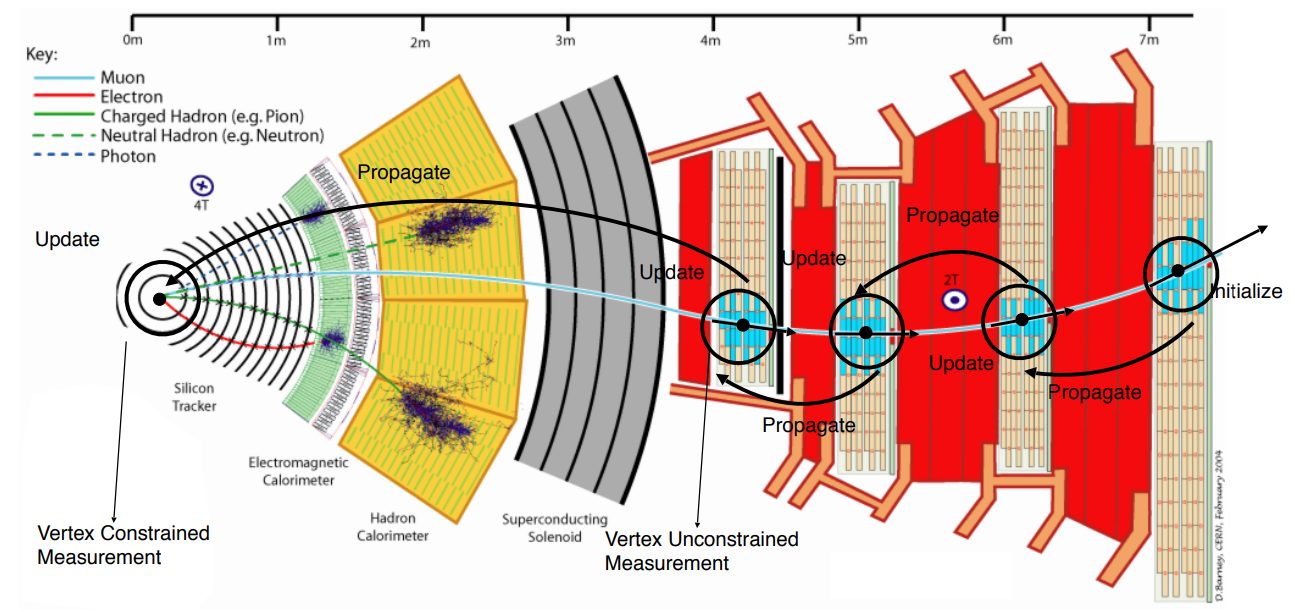
\includegraphics[width=0.85\linewidth]{figs/04_muons/kbmtf_diagram.png}
	\caption[The iterative process of propagation and updating a muon track through the KBMTF algorithm. The track properties at the innermost station are stored in order to trigger on muons not originating from the beam axis~\cite{CERN-LHCC-2020-004}]
	{The iterative process of propagation and updating a muon track through the KBMTF algorithm. The track properties at the innermost station are stored in order to trigger on muons not originating from the beam axis~\cite{CERN-LHCC-2020-004}.}
	\label{fig:kbmtf}
\end{figure}

\subsection{Muon Trajectory Propagation} \label{sec:muons_prop}
In order to implement a Kalman Filter, the propagation of muon tracks between stations must be expressed as a linear function of the track variables. From equation~\ref{eq:pt03br}, a charged particle will travel in a circular orbit in the $\hat{r}-\hat{\phi}$ plane. The high center of mass energy of the LHC results in highly energetic particles, whose trajectories have radii substantially larger than the size of the CMS detector. The large radius of curvature allows us to approximate these trajectories as parabolas. Assume a Cartesian coordinate system with the origin placed along a particle's trajectory that has radius R, as shown in figure~\ref{fig:mu_trajectory}. This trajectory can then be approximated as
\begin{equation}
	\label{eq:parabola1}
	y(x)=\frac{x^2}{2R}+bx
\end{equation}
where $b$ is a coefficient depending on the orientation of the coordinate system. If the initial trajectory is defined as $\phi_{b,0}$, taking the derivative and evaluating at the origin yields
\begin{equation}
	\label{eq:phib}
	b=\tan(\phi_{b,0})
\end{equation}	
The curvature $k=q/p_{T}$, where the muon charge $q=\pm1$, is the preferred variable to work with when propagating the trajectory of a muon, as the propagation is linear in $k$. Substituting values from equations~\ref{eq:pt03br} and~\ref{eq:phib} into equation~\ref{eq:parabola1} yields
\begin{equation}
	\label{eq:parabola2}
	y(x)=akx^2+\tan(\phi_{b,0})x
\end{equation}
where $a=\frac{0.3B}{2}$. Muon hits, or ``stubs'', provide information on the position $\phi$ and bending angle $\phi_b$. Let the radius of two sequential muon stations be $r_1$ and $r_2$, with the outer radius given by $r_2$ and $\Delta r=r_2-r_1$. Assuming a muon has curvature $k$ at the outer station and ignoring energy loss, equation~\ref{eq:parabola2} can be used to propagate stubs from the outer station towards the inner station.
\begin{equation}
	y(-\Delta r) = \left(a\Delta r^2\right)k-\Delta r\tan(\phi_{b,0})
\end{equation}
\begin{equation}
	y'(-\Delta r)=-\left(2a\Delta r\right)k+\tan(\phi_{b,0})
\end{equation}
Converting these quantities to the angles measured by the detector yields
\begin{equation}
	\label{eq:prop_phi}
	\Delta\phi=\mathrm{tan}^{-1}\left[\frac{y(-\Delta r)}{r_1}\right]
\end{equation}
\begin{equation}
	\label{eq:prop_phib}
	\phi_b=\Delta\phi+\mathrm{tan}^{-1}\left[y'(-\Delta r)\right]
\end{equation}
The $\Delta\phi$ term is added to equation~\ref{eq:prop_phib} because the bending angle at each station is measured relative to an axis system oriented towards the center of the detector. Due to the large radius of curvature of the muon trajectories, the small angle approximation $\tan(x)\sim \tan^{-1}(x)\sim x$ can be applied, giving the equations
\begin{equation}
	\label{eq:prop_phi_approx}
	\Delta\phi=\frac{a\Delta r^2}{r_1}k-\frac{\Delta r}{r_1}\phi_{b,0}
\end{equation}
\begin{equation}
	\label{eq:prop_phib_approx}
	\phi_b=a\Delta r\left(\frac{\Delta r}{r_1}-2\right)k+\left(\frac{r_2}{r_1}\right)\phi_{b,0}
\end{equation}
A diagram showing this propagation can be seen in figure~\ref{fig:mu_trajectory}.

\begin{figure}[h!]
	\centering
	%Final image: origin at outer stub, oriented with x axis pointing towards vertex
	% !TEX = root../../thesis.tex
\begin{tikzpicture}
	% axis system
	\draw[thick,->] (-11, 0) -- (1, 0) node[anchor=west] {x};
	\draw[thick,->] (0, 0) -- (0, 4) node[anchor=south] {y};
	\coordinate[label = above left:$\mathrm{Vertex}$] (vertex) at (-9.5, 0);
	\coordinate[label = above right:$\mathrm{Origin}$] (origin) at (0, 0);
	\coordinate[] (r1) at (-5, 0);
	\node at (vertex)[circle,fill,inner sep=2pt]{};
	\node at (origin)[circle,fill,inner sep=2pt]{};
	\draw[<->] (-9.5, -.5) -- (-5, -.5);
	\draw[<->] (-9.5, -1.1) -- (0, -1.1);
	\coordinate[label = below:$r_1$] (r1) at (-7.25,-.5);
	\coordinate[label = below:$r_2$] (r2) at (-5,-1.1);
	\draw[dashed] (-5, 0) -- (-5, 4);
	
	% muon trajectory
	\def \X{2.6047227}; %circle x0
	\def \Y{14.772116}; %circle y0
	
	\def \sy{1.8427620};%stub at (-5, y)
	\draw [{Latex[length=3mm]}-, domain=270:230] plot ({\X+15*cos(\x)}, {\Y+15*sin(\x)});
	\draw ({\X+15*cos(230)}, {\Y+15*sin(230)}) node[font=\bfseries, anchor=east] {$\mu$};
	\draw (-2.25,.25) node[anchor=west] {$\phi_{b,0}$};
	\coordinate[] (stub1) at (-5, \sy);
	\draw [dashed, domain=0:6] plot ({-9.5+\x}, {0.40950267*\x});
	\draw [dashed] (-5, \sy) -- (-4, \sy);
	\draw (-8.5, .25) node[anchor=west] {$\Delta\phi$};
	\draw (-4, \sy) node[anchor=west, scale=1.0] {$\phi_b$};
	\draw (-4.5, \sy+.1) node[anchor=west, scale=0.7] {$\Delta\phi$};
\end{tikzpicture}
	\caption{Diagram showing a muon trajectory between two stations with the origin set at the outer station. The x-axis is oriented using the detector vertex and the outer station.}
	\label{fig:mu_trajectory}
\end{figure}

Equations~\ref{eq:prop_phi_approx} - \ref{eq:prop_phib_approx} show that the track propagation fits the criteria for a discrete linear Kalman Filter discussed in section~\ref{sec:kalman_filter}. The matrices for propagation can now be constructed as follows. The transfer matrix $F_n$ from equation~\ref{eq:prop} can be expressed as
\begin{equation}
	\label{eq:kmtfProp}
	x_{n}=\left(\begin{matrix}
		k\\
		\phi\\
		\phi_b
	\end{matrix}\right)_{n} = 
\left(\begin{matrix}
	1 & 0 & 0\\
	\alpha_n & 1 & -\frac{\Delta r}{r_n}\\
	\beta_n & 0 & \frac{r_{n-1}}{r_n}
\end{matrix}\right)
\left(\begin{matrix}
	k\\
	\phi\\
	\phi_b
\end{matrix}\right)_{n-1}=F_nx_{n-1}
\end{equation}
where the coefficients
\begin{equation}
	\label{eq:kmtf_coeff}
	\alpha_n=a\frac{\Delta r^2}{r_n} \quad \mathrm{and} \quad \beta_n=a\Delta r\left(\frac{\Delta r}{r_n}-2\right)
\end{equation}
with $r_{n-1}$ being the radius of the previous (outer) muon station and $r_n$ the radius of the sequential (inner) muon station.

The propagation from the innermost station to the vertex has several differences to the propagation between muon stations. Energy loss is small but no longer negligible due to the amount of material from the tracker, ECAL, and HCAL. Recall that the track propagation occurs in reverse of the muon trajectory, so we must add energy when propagating to the vertex. Modeling the energy gain as a constant increase in momentum $p\to p+\varepsilon$, the curvature transforms as
\begin{equation}
	\label{eq:energygain}
	k=\frac{q}{p}\to\frac{q}{p+\varepsilon}=\frac{q/p}{1+\varepsilon/p}=\frac{k}{1+\varepsilon|k|}
\end{equation}
At the muon vertex, $\phi$ cannot be defined by the geometric position in the detector and is instead defined as the muon trajectory. Thus $\phi$ and $\phi_b$ at the muon vertex are the same by definition. Using equation~\ref{eq:parabola2}, we get
\begin{equation}
	\label{eq:vertex_phi}
	\phi\approx y'(-R)=-\alpha_0k+\phi_{b,0}
\end{equation}
where $R$ is the transverse distance from the beam axis to the innermost muon station and all coefficients of $k$ are absorbed into $\alpha_0$. Since $\phi_b$ propagation is now redundant, the bending angle then takes the role of \dxy. Accounting for energy loss, the \dxy is given by
\begin{equation}
	\label{eq:vertex_dxy}
	\dxy=y(-R)\approx \frac{\beta_0k}{1+\varepsilon|k|}-R\phi_{b,0}
\end{equation}
For simplifications in firmware calculations, we store the quantity $\dxy/R$ and account for the normalization when converting the digitized calculations to physical units.

While the radii of the muon stations are determined by detector geometry, the propagation constants  are measured using single muon monte-carlo samples where stubs are matched to the incident muons using generator level information. To determine $\alpha_n$, stubs in stations $n$ and $n-1$ are first associated if they resulted from the same incident muon. For matching stubs, the quantity $\Delta\phi+\frac{\Delta r}{r_1}\phi_{b,0}$ is plotted versus the muon $k$ at the outer station in a 2-dimensional histogram. Slices along the y-axis are fit using a Gaussian distribution, and the mean value for each slice is used to calculate a linear fit as a function of $k$. $\beta_n$ is calculated similarly by plotting $\phi_b-\left(r_{n-1}/r_n\right)\phi_{b,0}$ vs $k$. The process for calculating $\alpha_n$ can be seen in figure~\ref{fig:phi_prop}. For the vertex propagation, we plot $\phi_{gen}-\phi_b^\text{stub}$ versus $k$ to calculate $\alpha_0$. Lastly, the samples have exclusively prompt muons with $\dxy=0$, so we plot $\phi_b^\text{stub}$ versus $k$ to calculate $\beta_0$.

\begin{figure}[htb!]
	\centering
	\captionsetup{justification=centering}
	\begin{subfigure}[b]{0.45\textwidth}
		\centering
		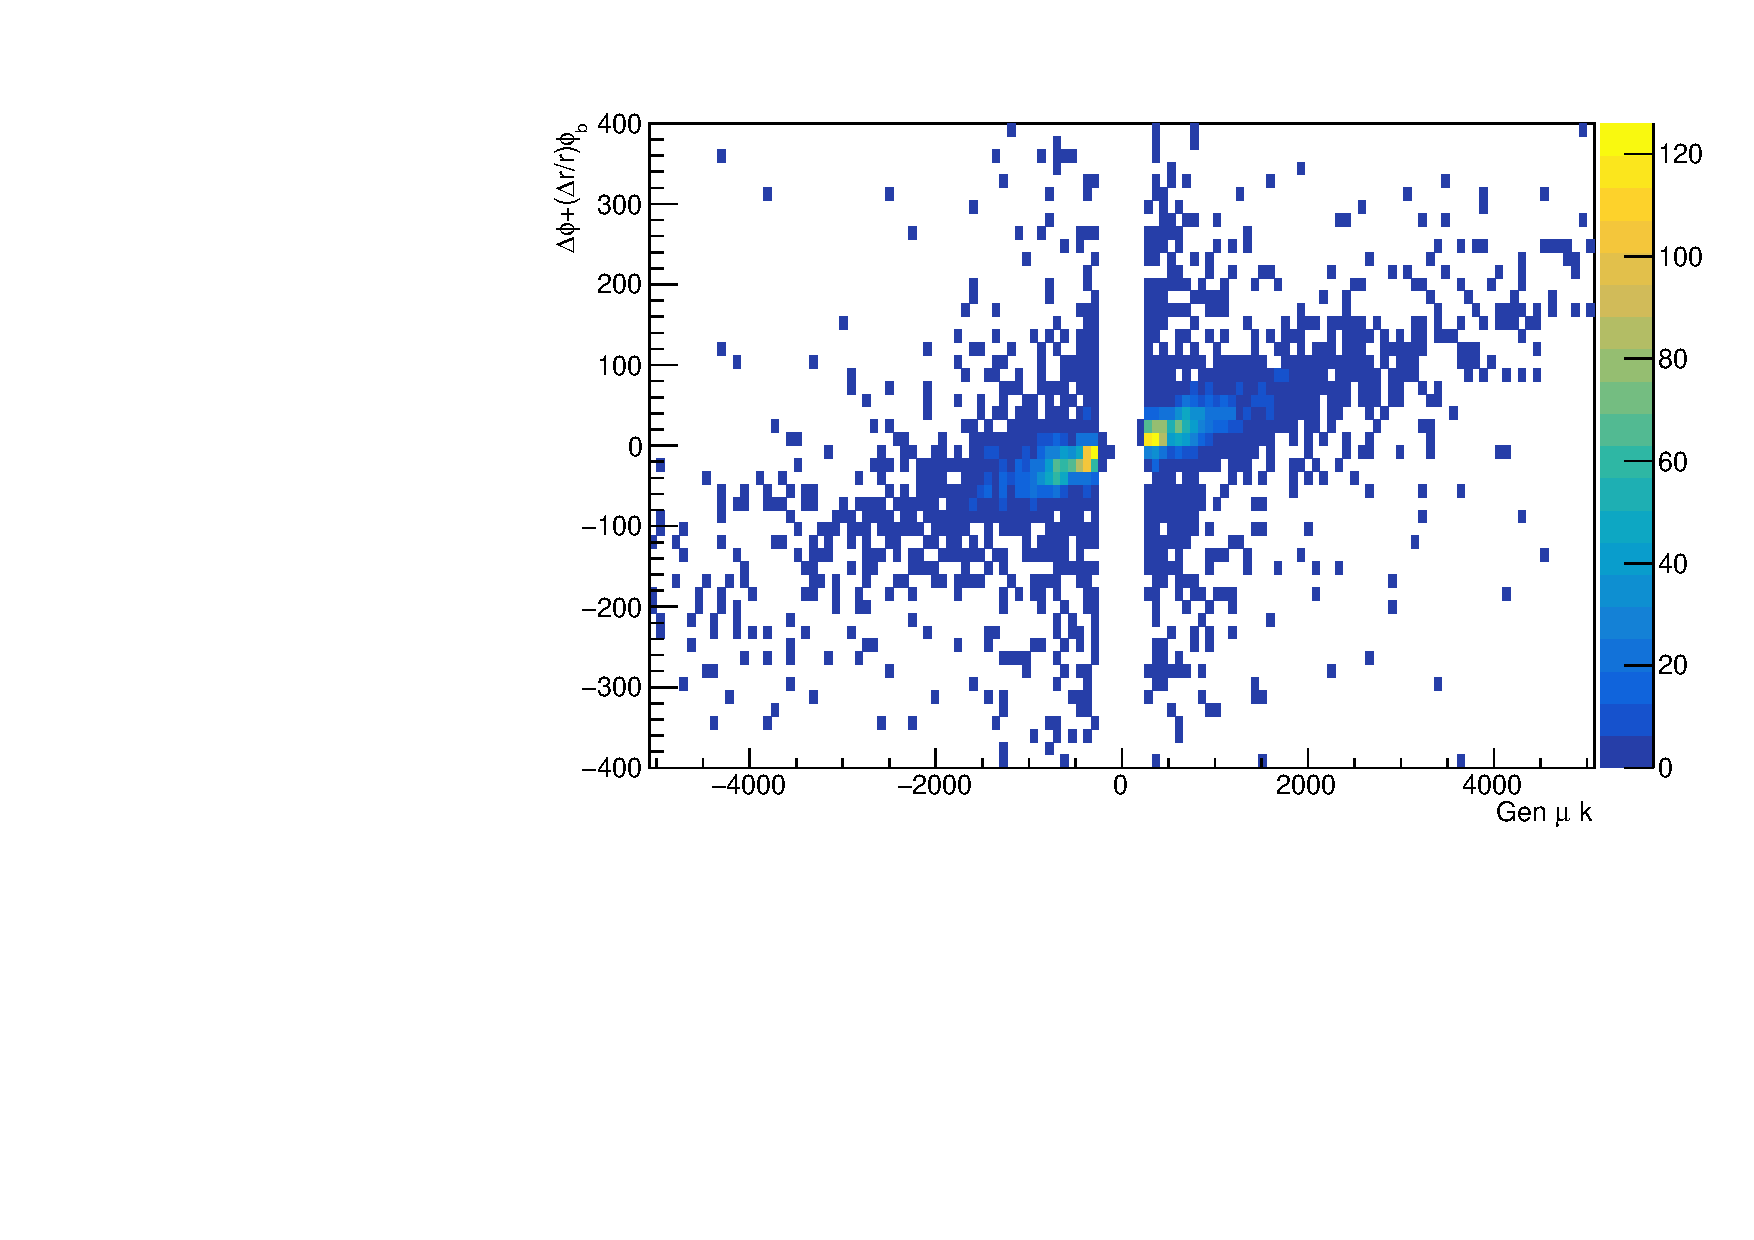
\includegraphics[width=\textwidth]{figs/04_muons/phiprop_2d.pdf}
		\caption{2-dimension histogram of $\Delta\phi+\frac{\Delta r}{r_1}\phi_{b,0}$ vs $k$.}
		\label{fig:2dprop}
	\end{subfigure}\hspace{0.05\textwidth}
	\begin{subfigure}[b]{0.45\textwidth}
		\centering
		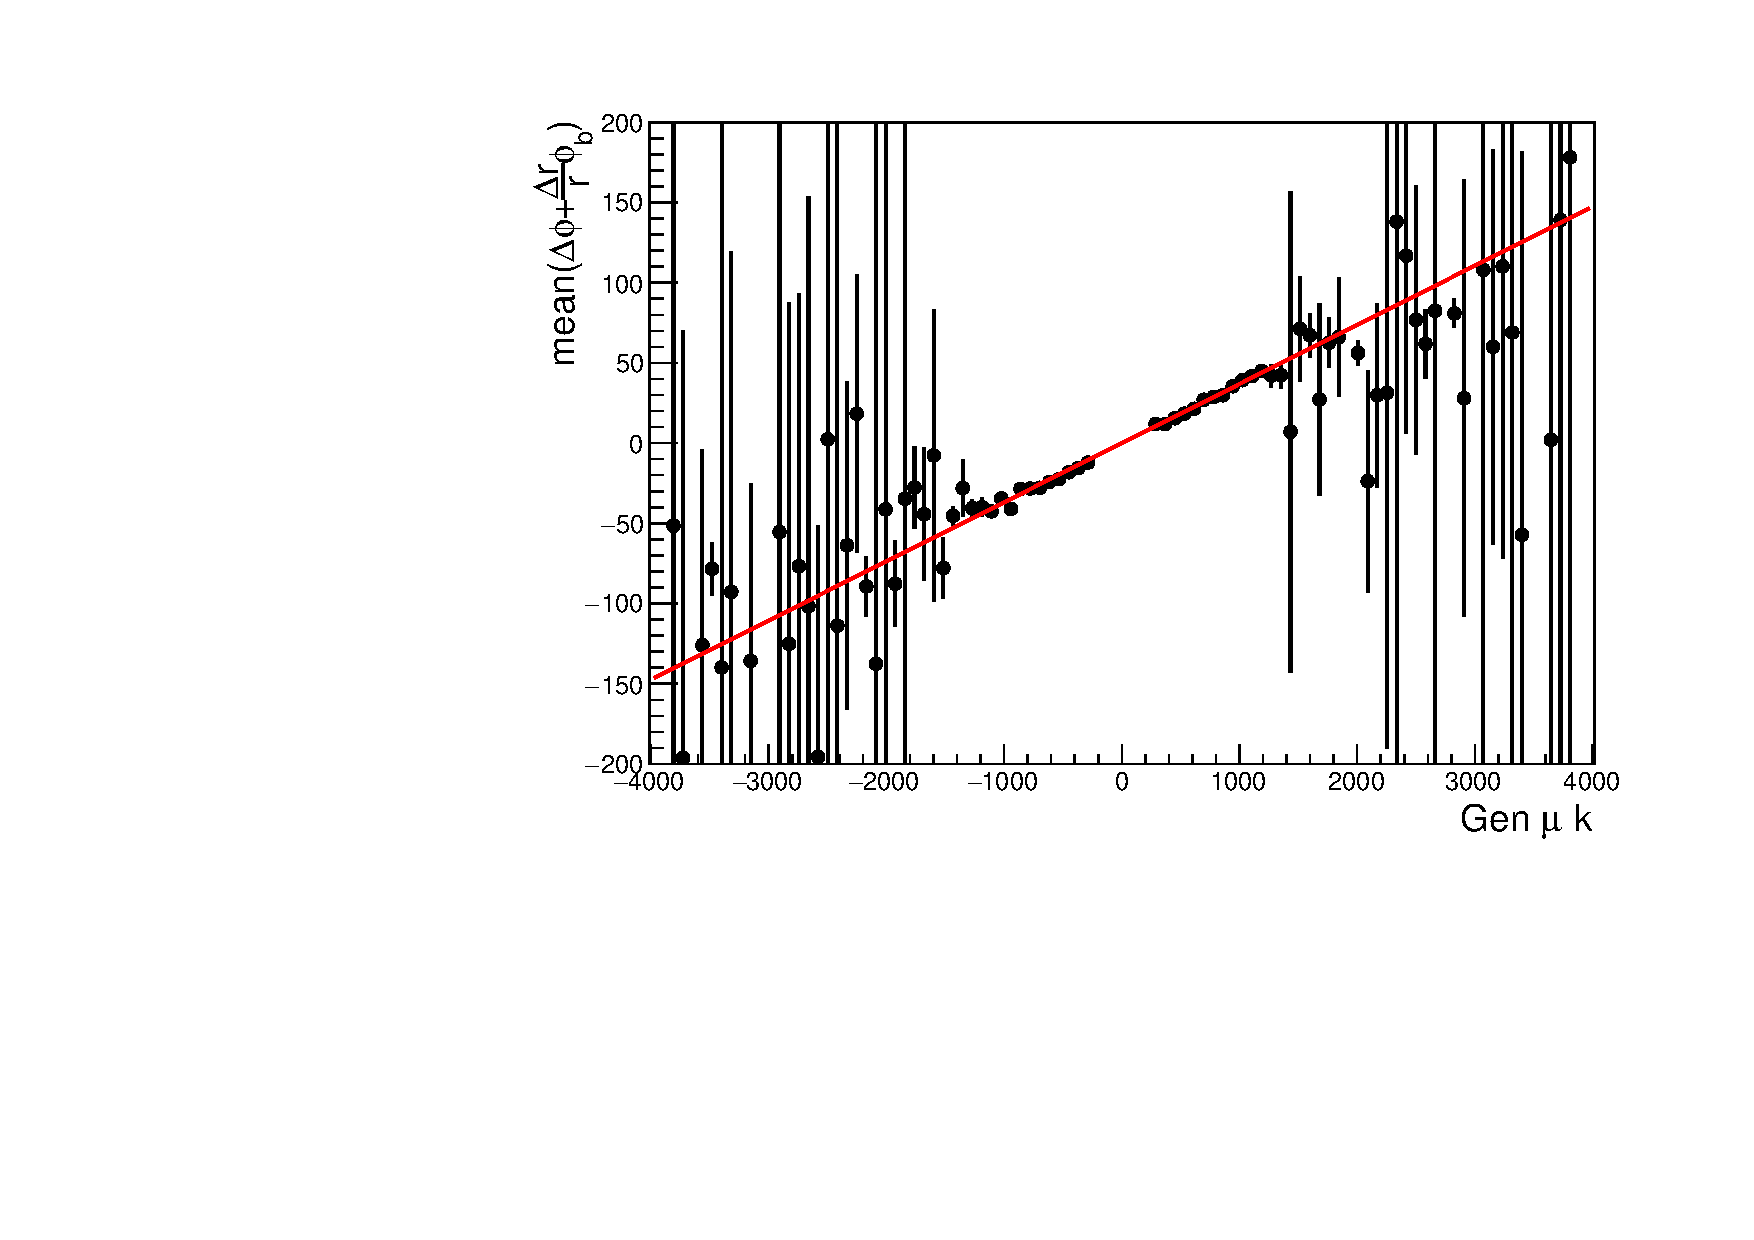
\includegraphics[width=\textwidth]{figs/04_muons/phiprop_mean.pdf}
		\caption{Mean of vertical slices fits used to calculate $\alpha$.}
		\label{fig:2dprop_mean}
	\end{subfigure}
	\caption[Calculation of phi propagation coefficients. Units are converted to their digitized form used in firmware calculations.]
	{Calculation of phi propagation coefficients. Units are converted to their digitized form used in firmware calculations.}
	\label{fig:phi_prop}
\end{figure}

\subsection{Covariant Matrices and the Kalman Gain} \label{sec:kbmtf_cov}
There are two sources of uncertainty that affect the covariance matrices. The first is multiple coulomb scattering, which occurs when muons scatter elastically with material in the detector. This can be thought of as a small deflection in momentum that alters the trajectory the muon. Lower momentum muons will be deflected at greater angles, so this uncertainty is proportional to $k$. Additionally, the probability for multiple scattering is proportional to the amount of material traversed by the muon, so this uncertainty must be calculated for each step in propagation. This is an uncertainty resulting from the propagation, and therefore plays the role of $Q_n$ from equation~\ref{eq:prop}. The second source is from the intrinsic detector resolution, which is a fixed value for each detector. However, the angular resolution is dependent on the radial distance from the center of the detector, so these must be calculated for each station as well. Since this is an uncertainty on the measurements, the resolution plays the role of $R_n$ in equation~\ref{eq:gain}. The total uncertainty resulting from both of these factors is given by
\begin{equation}
	\label{eq:prop_uncertainty}
	\sigma(k)=\sqrt{\sigma_{ms}^2k^2+\sigma_{res}^2}
\end{equation}

The coefficients can be calculated by using the Gaussian slice fits described when deriving $\alpha_n$ and $\beta_n$. For each propagation, the sigma of the Gaussian fits is plotted versus $k$ and fit to the form in equation~\ref{eq:prop_uncertainty}. This fitting process for $\phi$ propagation coefficients is shown in figure~\ref{fig:phi_uncertainty}, and is functionally the same for $\phi_b$.

\begin{figure}[htb!]
	\centering
	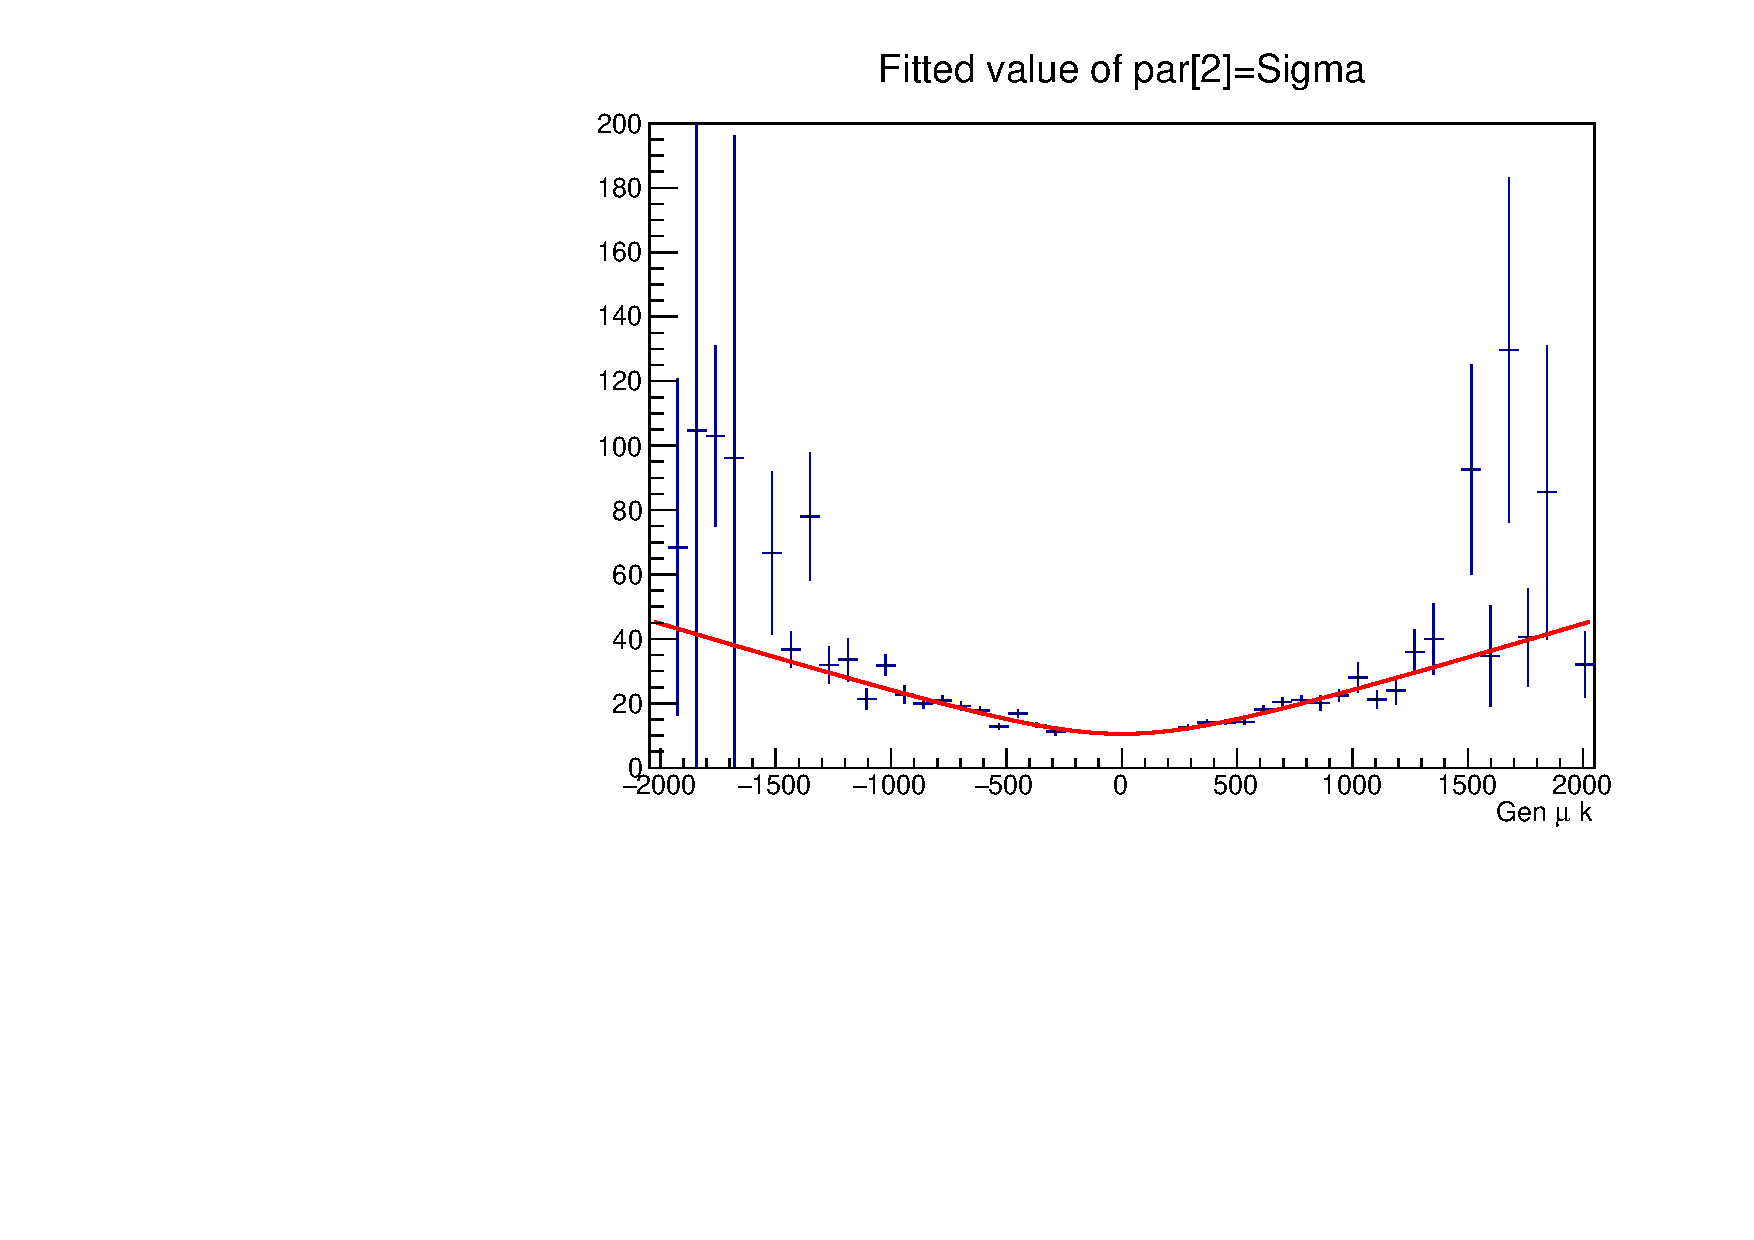
\includegraphics[width=0.45\linewidth]{figs/04_muons/phiprop_sigma.pdf}
	\label{fig:2dprop_sigma}
	\caption[$\sigma$ of vertical slice fits of the 2-dimensional histogram in figure~\ref{fig:2dprop} used to calculate uncertainty coefficients.]
	{$\sigma$ of vertical slice fits of the 2-dimensional histogram in figure~\ref{fig:2dprop} used to calculate uncertainty coefficients.}
	\label{fig:phi_uncertainty}
\end{figure}

Each stub has a measured value representing the ``quality'' of the hits, with higher values representing a more precise reconstruction of the bending angle. For this reason, the $\phi_b$ position resolutions are calculated separately for high and low quality stubs, as the uncertainty can differ by over a factor of 10 between the two. 

Since the muon detectors only measure $\phi$ and $\phi_b$, the matrix $H$ described in equation~\ref{eq:changeOfBasis} must be a 2$\times$3 matrix that takes the form
\begin{equation}
	H=\left(\begin{matrix}
		0 & 1 & 0\\
		0 & 0 & 1\end{matrix}\right)
\end{equation}

From this, the Kalman Gain $K'$ defined in equation~\ref{eq:gain2} must be a 3x2 matrix with indices $K_{ij}$, and the update step can be explicitly written as
\begin{align}
	\label{eq:kmtfUpdate}
	\begin{split}
	k_n^\mathrm{upd}&=k_{n-1}+K_{00}\Delta\phi+K_{01}\Delta\phi_b \\
	\phi_n^\mathrm{upd}&=\phi_n^\mathrm{prop}+K_{10}\Delta\phi+K_{11}\Delta\phi_b \\
	\phi_{b,n}^\mathrm{upd}&=\phi_{b,n}^\mathrm{prop}+K_{20}\Delta\phi+K_{21}\Delta\phi_b
	\end{split}
\end{align}
where $\Delta\phi$ and $\Delta\phi_b$ are the residuals for $\phi$ and $\phi_b$.

After the vertex propagation, there are no further muon stations to provide measurements for the update step. Instead, we assume a ``measurement'' of $\dxy=0$ with uncertainty given by the smallest non-zero value in the digitized units. $H$ is then a 1$\times$3 matrix, meaning the kalman gain $K'$ is a $3\times1$ matrix. The updated vertex coordinates are then
\begin{align}
	\label{eq:kmtfUpdate_vertex}
	\begin{split}
	k_\text{vertex}^\text{upd}&=k_\text{vertex}^\text{prop}+K_{00}\phi_b\\
	\phi_\text{vertex}^\text{upd}&=\phi_\text{vertex}^\text{prop}+K_{10}\phi_b\\
	\dxy^\text{upd}&=\dxy^\text{prop}+K_{20}\dxy^\text{prop}
	\end{split}
\end{align}
where the propagated curvature, $\phi$, and \dxy are given by equations~\ref{eq:energygain},~\ref{eq:vertex_phi}, and~\ref{eq:vertex_dxy}.

\subsection{Initial Curvature Assignment} \label{sec:kmtf_initk}
The propagation done by the KBMTF presupposes the curvature of the muon is known in order to calculate the $\phi$ and $\phi_b$ at the next station. In order to assign an initial value of the curvature to the track, we use the $\phi_b$ of the seed stub. Take a muon track beginning at the vertex, and align the axis so the initial bending angle $\phi_{b,0}=0$ as seen in figure~\ref{fig:mu_prop_vertex}. Equation~\ref{eq:parabola2} then becomes
\begin{equation}
	y(x)=akx^2
\end{equation}
From this, we can calculate the $\Delta\phi$ of the muon stub located a distance $R$ from the vertex as
\begin{equation}
	\Delta\phi\approx\frac{y(R)}{R}=akR\\
\end{equation}
The bending angle can then be calculated to be
\begin{equation}
	\label{eq:initPhiB}
	\phi_b\approx y'(R)-\Delta\phi=akR
\end{equation}

\begin{figure}[htb!]
	\centering
	% !TEX = root../../thesis.tex
\begin{tikzpicture}
	% axis system
	\draw[thick,->] (0,0) -- (10, 0) node[anchor=west] {x};
	\draw[thick,->] (0,-3) -- (0, 3) node[anchor=south] {y};
	\node at (0,0)[circle,fill,inner sep=2pt]{};
	\draw[{Latex[length=3mm]}-,domain=40:0] plot ({15*sin(\x)}, {15-15*cos(\x)});
	\draw ({15*sin(40)}, {15-15*cos(40)}) node[font=\bfseries,anchor=west]{$\mu$};

	\draw[<->] (0, -.5) -- (7, -.5);
	\coordinate[label=below:$R$] (r) at (3.4, -.5);
	\draw[dashed] (7, 0) -- (7, 3);
\end{tikzpicture}
	\caption[Coordinate system for muon propagation beginning at the vertex and going outward.]{Coordinate system for muon propagation beginning at the vertex and going outward.}
	\label{fig:mu_prop_vertex}
\end{figure}
From this, we can see that $\phi_b=\Delta\phi\propto k$. When propagating from the vertex, the muon undergoes small but non-negligable energy loss. Similar to equation~\ref{eq:energygain}, assume the energy loss can be modeled by a constant change in momentum $p\to p-\varepsilon$. Then the curvature $k$ goes as
\begin{equation}
	\label{eq:energyloss}
	k=\frac{q}{p}\to\frac{q}{p-\varepsilon}=\frac{q/p}{1-\varepsilon/p}=\frac{k}{1-\varepsilon |k|}
\end{equation}
In a similar process to the propagation coefficient calculation, we use simulated samples to plot $k$ versus $\phi_b$ for each station and fit it to the form
\begin{equation}
	k=\frac{a\phi_b}{1+b|\phi_b|}
\end{equation}
Each station then has coefficients $a$ and $b$ that are used to calculate the initial curvature from $\phi_b$.

Although the KBMTF is intended to be agnostic to the origin of the muon when reconstructing tracks, this derivation was done under the assumption that the muon originated from the vertex. We assign the initial curvature high uncertainty when setting the initial covariance matrix in order to avoid biasing the fit.

\subsection{Selection Criteria on Reconstructed Tracks} \label{sec:kmtf_qual}
The KBMTF requires reconstructed tracks to pass a minimum quality selection criteria in order to reject tracks from background, such as decayed hadrons that ``punch through'' the HCAL into the muon system. The first criteria measures the goodness of fit of the vertex unconstrained track by propagating the reconstructed track outward from the innermost station and measuring the difference in propagated and measured stub $\phi$ and $\phi_b$. Let the track at the innermost station have curvature, position, and bending angle given by $k$, $\phi^\text{track}$, and $\phi_b^\text{track}$. Applying equations~\ref{eq:prop_phi_approx} and~\ref{eq:prop_phib_approx} gives
\begin{equation}
	\label{eq:residual_prop}
	\left(\phi^\text{prop}-\phi^\text{track}\right)+\left(\phi_b^\text{prop}-\phi_b^\text{track}\right)=ck
\end{equation}
where $c$ is a constant depending on the propagation coefficients. The sum of residuals between stub and propagated coordinates is then 
\begin{align}
	\begin{split}
	\sum_{i\in\text{stubs}}\left(\phi^{\text{prop},i}-\phi^\text{i}\right)+\left(\phi_b^{\text{prop},i}-\phi_b^\text{i}\right)	&=\begin{multlined}[t]
									\sum_{i\in\text{stubs}}\left[(\phi^{\text{prop},i}-\phi^\text{track})+(\phi_b^{\text{prop},i}-\phi_b^\text{track})\right.\\
									+\left.(\phi^\text{track}-\phi^\text{i})+(\phi_b^\text{track}-\phi_b^\text{i})\right]
								\end{multlined}\\
 								& =\sum_{i\in\text{stubs}}c_ik+\left(\phi^\text{track}-\phi^\text{i}\right)+\left(\phi_b^\text{track}-\phi_b^\text{i}\right)
 	\end{split}
\end{align}
where $(\phi^i,\,\phi_b^i)$ are the position and bending angle of the $i$-th stub and $(\phi^{\text{prop},i},\,\phi_b^{\text{prop},i})$ are the position and bending angle of the track propagated to the $i$-th stub. The constants $c_i$ are derived using simulated samples by plotting $\Delta\phi+\Delta\phi_b$ versus $k$. The total residual sum is colloquially referred to as the approximate chi-square of the track. Tracks with three or more stubs must have an approximate chi-square below a preset threshold to be considered a candidate muon. The approximate chi-square is also used when overlap cleaning tracks that share stubs to determine which track to keep and which to reject.

A second quality cut, referred to as ``track compatibility'', measures the fit on the vertex constrained track. We propagate the vertex constrained track from the vertex to the highest quality stub (or outermost stub if multiple have equal quality), and compare the difference in $\phi_b^\text{prop}$ and $\phi_b^\text{stub}$ relative to the propagated $\phi_b^\text{prop}$ uncertainty. Equation~\ref{eq:initPhiB} shows that bending angle is proportional to the curvature of the muon at the vertex, with uncertainty from resolution and multiple scattering given by equation~\ref{eq:prop_uncertainty}. This gives $\phi_b^\text{prop}$ and $\sigma_{\phi_b}$ as
\begin{equation}
	\phi_b^\text{prop}=ck
\end{equation}
\begin{equation}
	\sigma_{\phi_b}=\sqrt{\sigma_\text{ms}^2k^2+\sigma_\text{res}^2}\approx\alpha|k|+\beta
\end{equation}
Using the Gaussian slice procedure described in section~\ref{sec:kbmtf_cov}, we use simulated samples to plot the curvature at the vertex $k$ versus stub bending angle $\phi_b^\text{stub}$. The means of the vertical slices are used to calculate $c$, while the sigma of the slices are used to calculate the uncertainty coefficients $\alpha$ and $\beta$. The track compatibility is then given by $|ck-\phi_b^\text{stub}|/(\alpha|k|+\beta)$. Tracks containing exactly two stubs must have a compatibility and approximate chi-square below a preset threshold, otherwise their vertex constrained momentum measurement is set to the minimum value. Changing the momentum as opposed to vetoing the track is done to keep the vertex unconstrained measurements unaffected in the event of real displaced muons, which would naturally have poor track compatibility after the vertex constraint.
% TODO: Should track compatibility account for energy loss

\subsection{Architecture of the KBMTF} \label{sec:kmtf_architecture}
The muon barrel detectors are segmented into 5 wheels along $\hat{z}$, which each wheel composed of 12 sectors in $\phi$ and each sector composed of 4 detector stations in $\hat{r}$, as shown in figure~\ref{fig:mu_barrel}.

\begin{figure}[htb!]
	\centering
	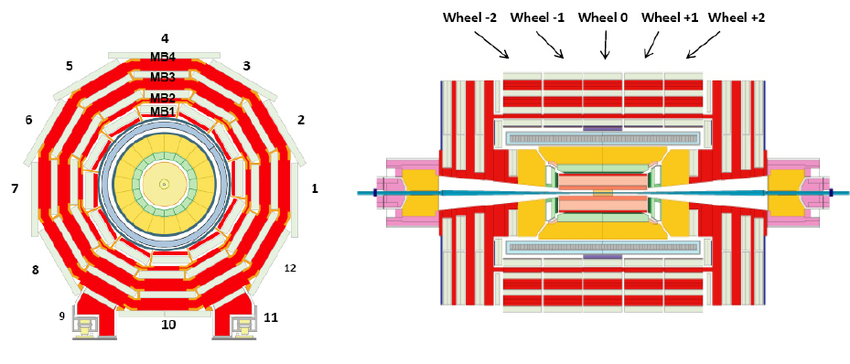
\includegraphics[width=.85\linewidth]{figs/04_muons/muon_barrel.png}
	\caption[Diagram of the CMS muon barrel system~\cite{Chatrchyan_2010}. (Left) $\hat{r}-\hat{\phi}$ slice showing the wheel segmented in 12 sectors in $\phi$ and 4 detector stations in $r$. (Right) $\hat{r}-\hat{z}$ slice showing the 5 wheels in $z$.]{Diagram of the CMS muon barrel system~\cite{Chatrchyan_2010}. (Left) $\hat{r}-\hat{\phi}$ slice showing the wheel segmented in 12 sectors in $\phi$ and 4 detector stations in $r$. (Right) $\hat{r}-\hat{z}$ slice showing the 5 wheels in $z$.}
	\label{fig:mu_barrel}
\end{figure}

The hardware for the KBMTF consists of 12 Master Processor --- Virtex-7 (MP7) boards, each hosting a Xilinx FPGA Virtex-7 690T chip, which are distributed among two $\mu$TCA crates~\cite{bmtf_hardware}. The FPGA is responsible for receiving inputs from the TwinMux system through high speed optical links, reconstructing muon tracks, and delivering the muon candidates to the global muon trigger. Each MP7 corresponds to a central wedge and receives TwinMux stubs from all stations in both the central wedge and the two adjacent wedges. We define a wedge as the adjacent sectors along all 5 wheels as shown in figure~\ref{fig:mu_wedge}. For a given MP7, the KBMTF algorithm reconstructs all tracks that have an outermost stub in the central wedge before overlap cleaning tracks that share stubs. It then picks the three best muon tracks based on track fit quality and \pt to deliver to the global muon trigger, where all muon candidates from the barrel, endcap, and overlap region are overlap cleaned and sorted.

\begin{figure}[htb!]
	\centering
	% !TEX = root = ../../thesis.tex
\usetikzlibrary{shapes.geometric}
\usetikzlibrary{calc}
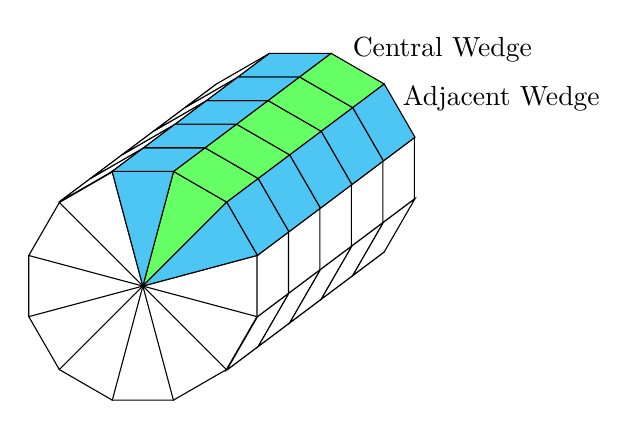
\begin{tikzpicture}

\def\dx{.4};
\def\dy{.3}
\def\r{3}
\def\c{1}
	
\node[draw, fill=white, regular polygon, regular polygon sides=12, minimum size=\r*\c cm] (w6) at (\dx*\c*5,\dy*\c*5){};
	
\node[draw, fill=white, regular polygon, regular polygon sides=12, minimum size=\r*\c cm] (w5) at (\dx*\c*4,\dy*\c*4){};

\node[draw, fill=white, regular polygon, regular polygon sides=12, minimum size=\r*\c cm] (w4) at (\dx*\c*3,\dy*\c*3){};

\node[draw, fill=white, regular polygon, regular polygon sides=12, minimum size=\r*\c cm] (w3) at (\dx*\c*2,\dy*\c*2){};

\node[draw, fill=white, regular polygon, regular polygon sides=12, minimum size=\r*\c cm] (w2) at (\dx*\c*1,\dy*\c*1){};

\node[draw, fill=white, regular polygon, regular polygon sides=12, minimum size=\r*\c cm] (w1) at (0,0){};

\foreach \i in {1,2,3,4,5,6,7,8,9,10,11,12}{
	\draw (0,0) -- (w1.corner \i);
}
\foreach \i in {1,2,3,9,10,11,12}{
	\draw (w1.corner \i) -- (w6.corner \i);
}


% Fixing perspective
\draw[fill=white] (w1.corner 9) -- (w2.corner 9) -- (w2.corner 10) -- (w1.corner 10) -- cycle;
\draw[fill=white] (w2.corner 9) -- (w3.corner 9) -- (w3.corner 10) -- (w2.corner 10) -- cycle;
\draw[fill=white] (w3.corner 9) -- (w4.corner 9) -- (w4.corner 10) -- (w3.corner 10) -- cycle;
\draw[fill=white] (w4.corner 9) -- (w5.corner 9) -- (w5.corner 10) -- (w4.corner 10) -- cycle;
\draw[fill=white] (w5.corner 9) -- (w6.corner 9) -- (w6.corner 10) -- (w5.corner 10) -- cycle;

\draw[fill=white] (w1.corner 2) -- (w2.corner 2) -- (w2.corner 3) -- (w1.corner 3) -- cycle;
\draw[fill=white] (w2.corner 2) -- (w3.corner 2) -- (w3.corner 3) -- (w2.corner 3) -- cycle;
\draw[fill=white] (w3.corner 2) -- (w4.corner 2) -- (w4.corner 3) -- (w3.corner 3) -- cycle;
\draw[fill=white] (w4.corner 2) -- (w5.corner 2) -- (w5.corner 3) -- (w4.corner 3) -- cycle;
\draw[fill=white] (w5.corner 2) -- (w6.corner 2) -- (w6.corner 3) -- (w5.corner 3) -- cycle;

% Central wedge
\draw[fill=green!60] (w1.corner 12) -- (w1.corner 1) -- (0,0) -- cycle;
\draw[fill=green!60] (w1.corner 12) -- (w2.corner 12) -- (w2.corner 1) -- (w1.corner 1) -- cycle;
\draw[fill=green!60] (w2.corner 12) -- (w3.corner 12) -- (w3.corner 1) -- (w2.corner 1) -- cycle;
\draw[fill=green!60] (w3.corner 12) -- (w4.corner 12) -- (w4.corner 1) -- (w3.corner 1) -- cycle;
\draw[fill=green!60] (w4.corner 12) -- (w5.corner 12) -- (w5.corner 1) -- (w4.corner 1) -- cycle;
\draw[fill=green!60] (w5.corner 12) -- (w6.corner 12) -- (w6.corner 1) -- (w5.corner 1) -- cycle;

% Adjacent wedge +1
\draw[fill=cyan!70] (w1.corner 11) -- (w1.corner 12) -- (0,0) -- cycle;
\draw[fill=cyan!70] (w1.corner 12) -- (w2.corner 12) -- (w2.corner 11) -- (w1.corner 11) -- cycle;
\draw[fill=cyan!70] (w2.corner 12) -- (w3.corner 12) -- (w3.corner 11) -- (w2.corner 11) -- cycle;
\draw[fill=cyan!70] (w3.corner 12) -- (w4.corner 12) -- (w4.corner 11) -- (w3.corner 11) -- cycle;
\draw[fill=cyan!70] (w4.corner 12) -- (w5.corner 12) -- (w5.corner 11) -- (w4.corner 11) -- cycle;
\draw[fill=cyan!70] (w5.corner 12) -- (w6.corner 12) -- (w6.corner 11) -- (w5.corner 11) -- cycle;
% Adjacent wedge -1

\draw[fill=cyan!70] (w1.corner 1) -- (w1.corner 2) -- (0,0) -- cycle;
\draw[fill=cyan!70] (w1.corner 2) -- (w2.corner 2) -- (w2.corner 1) -- (w1.corner 1) -- cycle;
\draw[fill=cyan!70] (w2.corner 2) -- (w3.corner 2) -- (w3.corner 1) -- (w2.corner 1) -- cycle;
\draw[fill=cyan!70] (w3.corner 2) -- (w4.corner 2) -- (w4.corner 1) -- (w3.corner 1) -- cycle;
\draw[fill=cyan!70] (w4.corner 2) -- (w5.corner 2) -- (w5.corner 1) -- (w4.corner 1) -- cycle;
\draw[fill=cyan!70] (w5.corner 2) -- (w6.corner 2) -- (w6.corner 1) -- (w5.corner 1) -- cycle;

%\node[text=green!60, label={right:Central Wedge}] at ($(w6.corner 12)!0.5!(w6.corner 1)$){};
\node[label={[right]:Central Wedge}, xshift=1ex, yshift=-.5ex] at (w6.corner 1){};
\node[label={[right]:Adjacent Wedge},xshift=0.75ex, yshift=-2ex] at (w6.corner 12){};

\end{tikzpicture}

	\caption[Diagram showing the inputs of one MP7 board, consisting of the TwinMux inputs from one central wedge (green) and the two adjacent wedges (blue). The KBMTF reconstructs all tracks with the outermost stub in the central wedge.]{Diagram showing the inputs of one MP7 board, consisting of the TwinMux inputs from one central wedge (green) and the two adjacent wedges (blue). The KBMTF reconstructs all tracks with the outermost stub in the central wedge.}
	\label{fig:mu_wedge}
\end{figure}

\subsection{Firmware Implementation of the KBMTF} \label{sec:fw}
Two minor approximations are made in order to reduce algorithmic latency and memory usage for firmware implementation. The position resolution of $\phi$ is substantially smaller than the multiple scattering resolution, so the track $\phi$ is set automatically to the measured stub $\phi$. This is equivalent to fixing $K_{10}=1$ and $K_{11}=0$ in equation~\ref{eq:kmtfUpdate}. Secondly, due to the high uncertainty associated with both the measured and propagated $\phi_b$, tracks using three or more stubs set $K_{i1}$ equal to zero and only update using the residual from $\phi$.

Although the Kalman Gain can be exactly calculated exactly given the covariance matrices using equation~\ref{eq:gain}, matrix inversion is a resource and latency expensive process for the hardware based trigger. Implementing division into hardware is significantly more resource intensive than multiplication, so the calculation of the determinant, which requires matrix inversions, would cause the algorithm to exceed the latency requirements for real time track finding. Instead, the values of $K_{ij}$ are stored in look-up tables (LUTs) as a function of curvature and the combination of stations that were used to update the track, referred to as the track pattern. For tracks with only two stubs, the LUT contains the exact values of the gain that would have been calculated using equation~\ref{eq:gain2}. For tracks with more than two stubs, this is an approximation that loses some information from updates at previous stations but produces nearly identical performance.

When propagating $k$ and \dxy to the vertex, the energy loss would require division to calculate in real time. Therefore we store the values for $k/(1+\epsilon|k|)$ in LUTs for each value of $k$. Additionally, the $\phi$ is not propagated to or updated at the vertex; instead we define the $\phi$ of the track using the stub $\phi$ at station 2, or the propagated phi at station 2 if no stub exists. Lastly, the vertex update is only performed on the curvature, since the $\dxy$ is only important for the unconstrained measurement.

As outlined in section~\ref{sec:kbmtf_cov}, the $\phi_b$ resolution coefficients are different for high and low quality stubs, thus the values for $K_{ij}$ would have to be provided for every possible combination of high and low quality stubs for each track pattern. This would exponentially increase the number of gains stored on LUTs beyond the memory capacity of the hardware. However, from previous approximations, residuals for $\phi_b$ are not used for tracks containing three or more stubs, which fixes $K_{01}$ and $K_{21}$ at 0 for these track patterns. Only gains for track patterns containing two stubs must account for the quality of the stubs. With four stations, this yields six track patterns with four combinations of stub quality that must be stored in LUTs, which is within the capacity of the current hardware.

The firmware is written using Vivado High Level Synthesis (HLS) which compiles firmware written in C to HDL, optimizing it for a given FPGA and clock frequency~\cite{Bachtis:2648953}. When synthesized in a Virtex 7 690T FPGA with a clock frequency of 160\unit{MHz}, the KBMTF algorithm can process a single event in 9 bunch crossings, and is pipelined to allow for continuous processing of events. Table~\ref{tab:kmtfFW} shows the resource utilization of the KBMTF compared to the previous BMTF algorithm, which was implemented using an identical FPGA and clock frequency.

\begin{table} [htb!]
	\centering
	\begin{tabular}{|l|r r r r|}
	\hline
	Algorithm & LUT & FF & BRAM & DSP \\
	\hline
	Phase I BMTF & 43\% & 23\% & 35\% & 0\%\\
	KBMTF & 16\% & 11\% & 15\% & 25\% \\
	\hline 
	\end{tabular}
	\caption[Comparison of resource utilization on a Virtex 7 690T FPGA~\cite{CERN-LHCC-2020-004}. The KBMTF utilizes DSP cores for arithmetic operations to propagate and update tracks and LUTs for the propagation coefficients and approximate Kalman Gain, while the BMTF uses LUTs to assign momentum.]
	{Comparison of resource utilization on a Virtex 7 690T FPGA~\cite{CERN-LHCC-2020-004}. The KBMTF utilizes DSP cores for arithmetic operations to propagate and update tracks and LUTs for the propagation coefficients and approximate Kalman Gain, while the BMTF uses LUTs to assign momentum.}
	\label{tab:kmtfFW}
\end{table}

\section{Performance of the Kalman Barrel Muon Track Finder} \label{sec:kmtf_performance}
The performance of a trigger algorithm is primarily determined by the rate and efficiency. The efficiency is the fraction of signal events that successfully have a track reconstructed by the algorithm, while the rate is the frequency that the algorithm will trigger. A high efficiency is desirable to ensure any interesting events are stored for future analysis, while a low rate is crucial to reject background events and provide a reasonable bandwidth to store events.

The Phase-I BMTF functioned by using pairs of stubs to form tracks, then using a LUT to assign track parameters based on the $\phi$ and $\phi_b$ of the stubs. This LUT uses only the $\phi$ and $\phi_b$ of the two stubs and was derived with the assumption that the muon originated from the beam axis. The KBMTF utilizes the full detector information to reconstruct muons, leading to higher efficiency and lower rate than the BMTF. In the case of displaced muons, which arise from secondary decays of long lived, beyond standard model particles, the BMTF beam axis assumption is no longer valid and results in large inefficiencies as the muon becomes more displaced, while the KBMTF provides vertex unconstrained measurements resulting in substantial gains to efficiency.

\subsection{Trigger Efficiencies} \label{sec:kmtf_eff}
The general efficiency of a trigger is defined as the fraction of signal muons that have a matching reconstructed track, and can be expressed abstractly as
\begin{equation}\label{eq:eff}
	\epsilon=\frac{N_\mathrm{signal}(\mathrm{Passing\ trigger})}{N_\mathrm{signal}}	
\end{equation}
The uncertainty of an efficiency cannot be calculated using the propagation of uncorrelated Poisson errors, as the number of passing events follows a binomial distribution. Although these converge asymptotically for large $N$, at small $N$ it is possible to have an upper confidence limit $>1$, which would be a non-physical value for an uncertainty. Instead, we utilize the Clopper-Pearson confidence intervals for binomial distributions~\cite{clopperpearson}. For a significance of $\alpha$, the confidence interval is given by $(\epsilon_\text{low}, \epsilon_\text{up})$ which satisfy
\begin{align}
		\frac{\alpha}{2}&=\frac{\Gamma(N+1)}{\Gamma(x)\Gamma(N-x-1)}\int_{0}^{\epsilon_\text{low}}t^{x-1}(1-t)^{N-x}dt=I_{\epsilon_\text{low}}(x,N-x+1)\\
		1-\frac{\alpha}{2}&=\frac{\Gamma(N+1)}{\Gamma(x+1)\Gamma(N-x)}\int_{0}^{\epsilon_\text{up}}t^x(1-t)^{N-x-1}dt=I_{\epsilon_\text{up}}(x+1,N-x)
\end{align}
where $x$ is the number of passed events, $N$ is the total number of events, and $I_\epsilon(\alpha,\beta)$ is the regularized incomplete beta function. Clopper-Pearson error bars for a confidence level of $(1-0.68)$ are drawn automatically through the use of the \texttt{TGraphAsymmetricErrors} class in ROOT.

For muon triggers, the denominator of signal muons consist of events that have known information about the muons. This can be from generator information in simulated monte-carlo samples, tracker information using cosmic muon data, or probe muons using the tag-and-probe method on data. These signal muons are cut using the known muon information to produce a reasonable sample for track reconstruction. The numerator consists of signal muons with a matching reconstructed track that may have addition cuts on the reconstructed track properties.

Figure~\ref{fig:eff_KmtfVsBmtf} shows the efficiencies calculated on probe muons from a Z boson tag-and-probe sample collected during 2017 data taking. The associated tracker tracks for the probe muons are used as the known information, while the associated stubs are used to run the L1 muon reconstruction algorithms. Figure~\ref{fig:effVsPt} shows the efficiency versus track \pt comparing the KBMTF and phase-1 BMTF algorithm, with the requirement that the matching L1 muons have $\pt>20\GeV$. This requirement creates the turn-on curve effect, which has a sharpness proportional to the muon momentum resolution, followed by the plateau at which the algorithms reach maximum efficiency. Figure~\ref{fig:effVsEta} shows the same efficiencies versus track $\eta$, with the additional requirement that the tracker tracks have $\pt>25\GeV$ in order to show the efficiency on the plateau. Quality cuts in the KBMTF algorithm were tuned to match the efficiency of the BMTF.

\begin{figure}[htb!]
	\centering
	\captionsetup[subfigure]{justification=centering}
	\begin{subfigure}[h]{0.45\linewidth}
		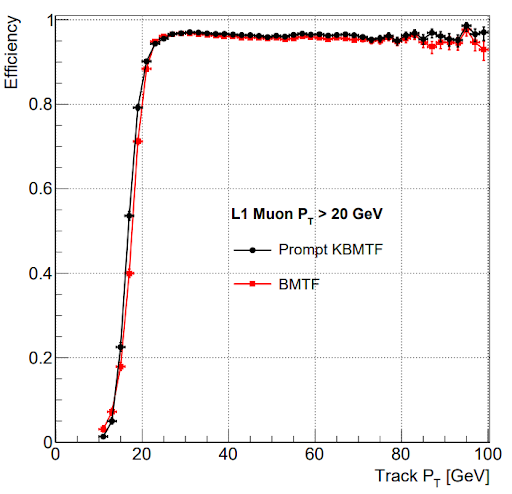
\includegraphics[width=\linewidth]{figs/04_muons/effVsPt_kmtf.png}
		\caption{Efficiency versus track \pt}
		\label{fig:effVsPt}
	\end{subfigure}
	\begin{subfigure}[h]{0.45\linewidth}
		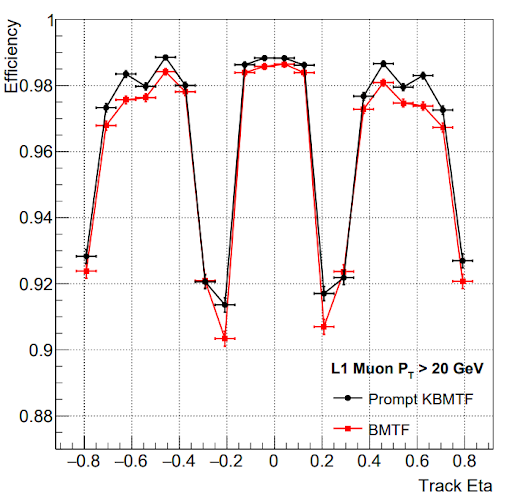
\includegraphics[width=\linewidth]{figs/04_muons/effVsEta_kmtf.png}
		\caption{Efficiency versus track $\eta$}
		\label{fig:effVsEta}
	\end{subfigure}
	\caption[Comparison of efficiencies between the KBMTF and phase-1 BMTF algorithm using a Z tag-and-probe sample collected during 2017 data taking. (a) Efficiency versus track \pt, requiring L1 muon $\pt>20\GeV$. (b) Efficiency versus track $\eta$, requiring L1 muon $\pt>20\GeV$ and track $\pt>25\GeV$ in order to show the efficiency on the plateau. The drops in efficiency at $\eta=\pm0.2$ are due to gaps between wheels in the muon system.]{Comparison of efficiencies between the KBMTF and phase-1 BMTF algorithm using a Z tag-and-probe sample collected during 2017 data taking. (a) Efficiency versus track \pt, requiring L1 muon $\pt>20\GeV$. (b) Efficiency versus track $\eta$, requiring level-1 muon $\pt>20\GeV$ and track $\pt>25\GeV$ in order to show the efficiency on the plateau. The drops in efficiency at $\eta=\pm0.2$ are due to gaps between wheels in the muon system.}
	\label{fig:eff_KmtfVsBmtf}
\end{figure}

Figure~\ref{fig:effVsDxy_kmtf} shows the efficiency versus muon $d_{xy}$ for three track finding algorithms. The denominator consists of cosmic ray muons passing through the barrel muon detectors with a $p_T>20\GeV$. The numerator requires a matching L1 track with reconstructed $p_T>10\GeV$. The lower threshold for the L1 track is set to prevent the momentum resolution of the reconstruction algorithms from affecting the efficiency. The first algorithm is the BMTF, which shows inefficiencies due to the $p_T$ LUTs assuming the muon originated at the beam axis. The second is the prompt KBMTF, which uses the vertex constrained measurement. This also shows inefficiencies due to the vertex constraint, but is better than the BMTF as the vertex constraint isn't applied until the last step of track reconstruction. Lastly, the displaced KBMTF uses the vertex unconstrained measurement and shows substantial improvements compared to both prompt algorithms.

\begin{figure}[htbp!]
	\centering
	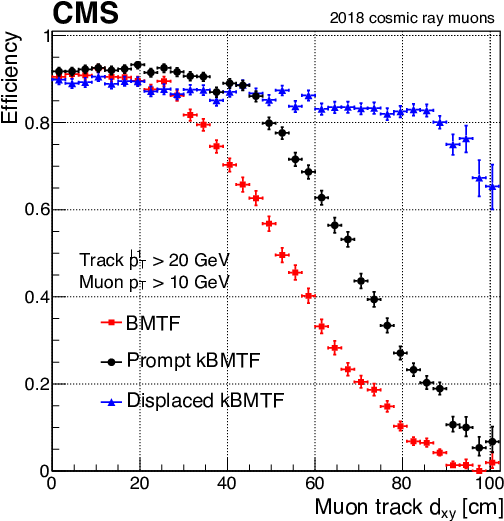
\includegraphics[width=0.5\linewidth]{figs/04_muons/effVsDxy_kmtf.png}
	\caption[Comparison of efficiency vs cosmic track $d_{xy}$ using cosmic data from the 2018 data taking run. The prompt KBMTF takes the reconstructed $p_{T}$ using the vertex constrained measurement, while the displaced KBMTF uses the vertex unconstrained measurement. The displaced KBMTF shows substantial improvements to the previous BMTF~\cite{Hayrapetyan:2870088}]
	{Comparison of efficiency vs cosmic track $d_{xy}$ using cosmic data from the 2018 data taking run. The prompt KBMTF takes the reconstructed $p_{T}$ using the vertex constrained measurement, while the displaced KBMTF uses the vertex unconstrained measurement. The displaced KBMTF shows substantial improvements to the previous BMTF~\cite{Hayrapetyan:2870088}.}
	\label{fig:effVsDxy_kmtf}
\end{figure}

\subsection{Trigger Rates} \label{sec:kmtf_rate}
A reconstructed muon must have a $p_T$ above a given threshold to trigger on an event. Thresholds are set to optimize the analysis potential of the data while also minimizing the additional bandwidth to store events. The rate, which is the frequency at which a trigger decides to store an event, can be calculated as a function of threshold using zero bias data, which is collected by storing random events regardless of trigger acceptance. This creates a representative data set of all $pp$ collisions, hence the name ``zero bias''. The rate can be calculated from the zero bias data as follows
\begin{equation}
	\mathrm{R} = f_\mathrm{rev}\times \left<N_\mathrm{bunches}\right>\times\frac{N_\mathrm{events}(\mathrm{L1}\ \mathrm{Track}\ p_{T}>\mathrm{Threshold})}{N_\mathrm{events}}
\end{equation}
Where $f_\mathrm{rev}$ is the LHC revolution frequency of 11.245\unit{kHz} and $\left<N_\mathrm{bunches}\right>$ is the average number of proton bunches that will collide in one revolution. For 2017 data taking these yield a scale factor of 20984$\unit{kHz}$. Figure~\ref{fig:kmtf_rate} shows the rate versus threshold for the BMTF, vertex constrained KBMTF, and vertex unconstrained KBMTF. The KBMTF was tuned for similar efficiency but lower rate than the BMTF at 20\GeV. The displaced KBMTF initially shows lower rate at low \pt thresholds due to scale corrections to the reconstructed muon momentum.

\begin{figure}[htbp!]
	\centering
	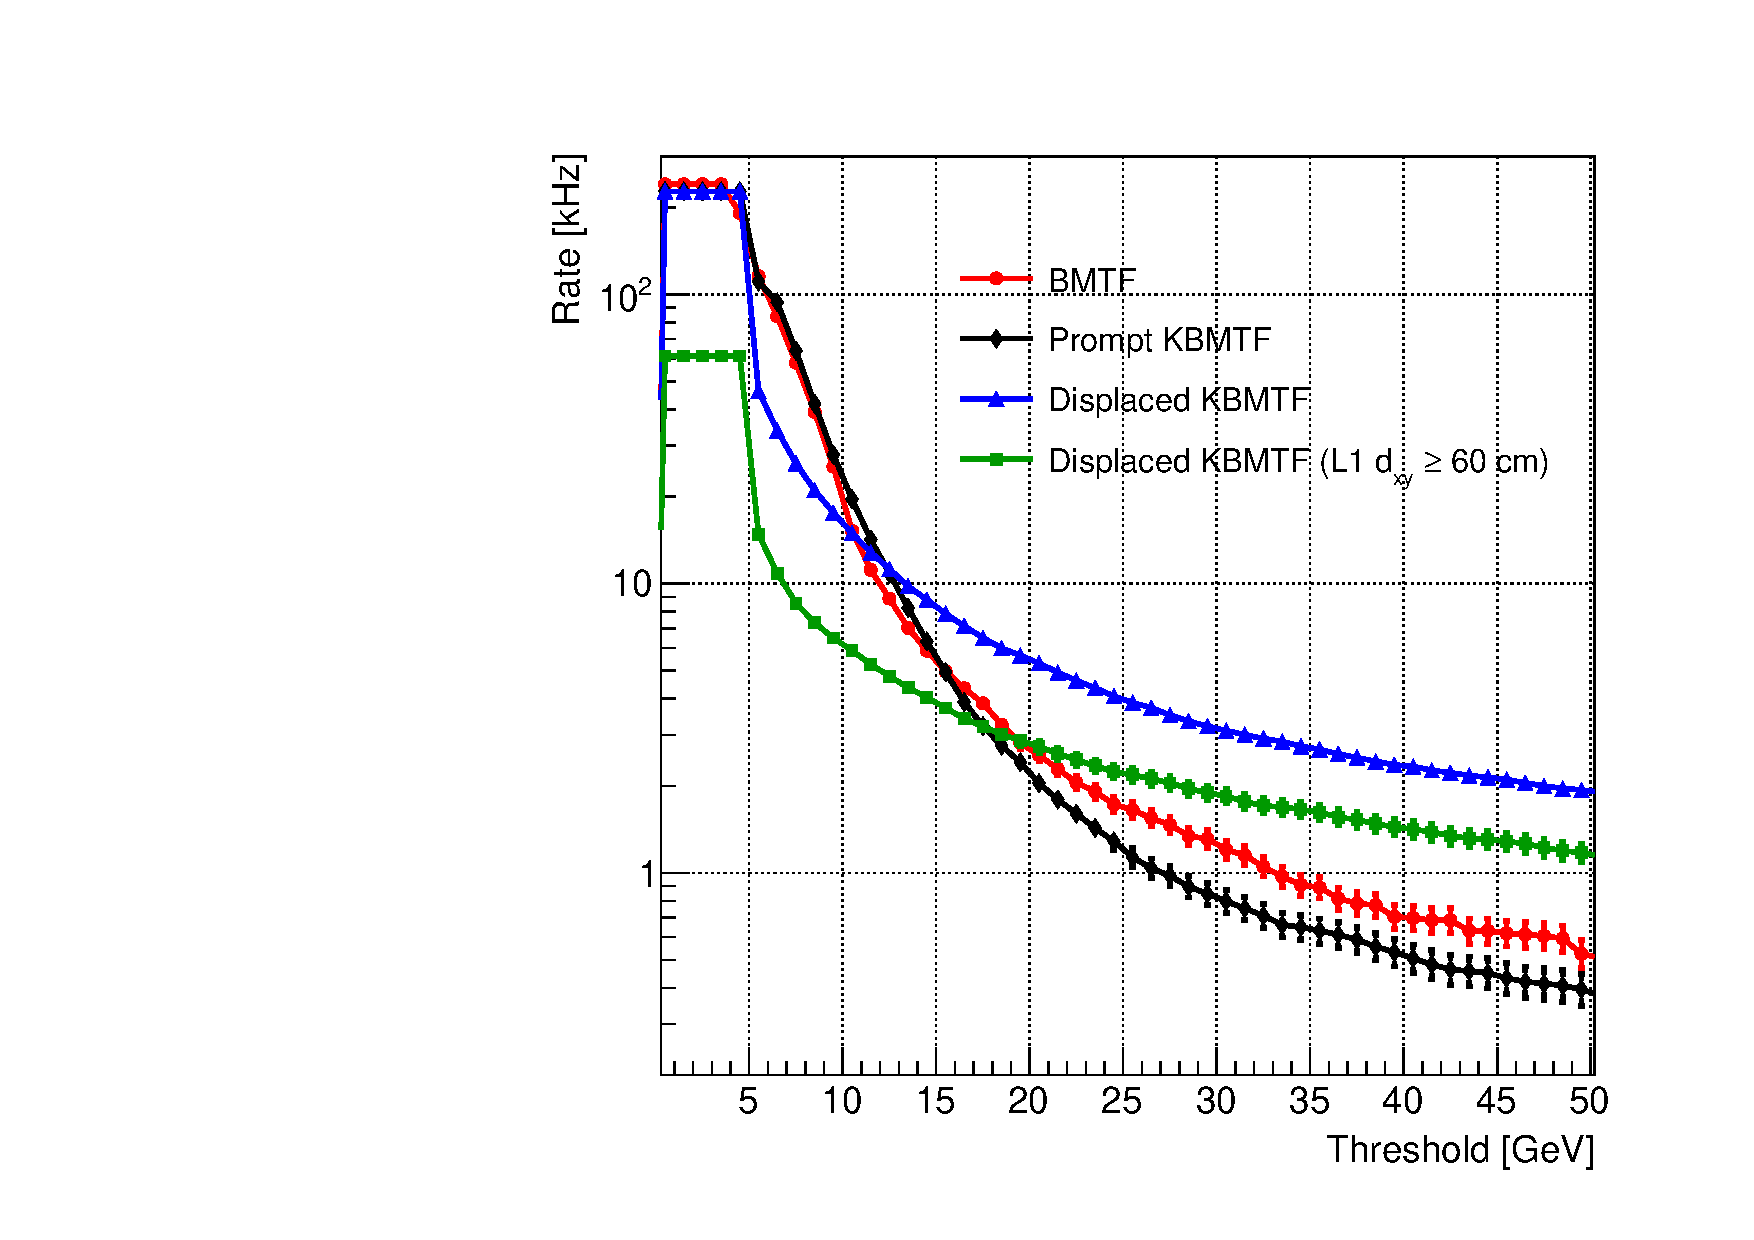
\includegraphics[width=0.5\linewidth]{figs/04_muons/rate_kmtf.pdf}
	\caption[Rate comparison calculated using 2017 zero bias data of the Phase I BMTF, vertex constrained (prompt) KBMTF, vertex unconstrained (displaced) KBMTF, and displaced KBMTF for displaced tracks.]{Rate comparison calculated using 2017 zero bias data of the Phase I BMTF, vertex constrained (prompt) KBMTF, vertex unconstrained (displaced) KBMTF, and displaced KBMTF for displaced tracks.}
	\label{fig:kmtf_rate}
\end{figure}

\subsection{Firmware and Emulator Agreement} \label{sec:kmtf_fwVsEmu}
The performance of the KBMTF is tested using a dedicated C++ software emulator which is integrated into the CMS analysis framework. This emulator follows similar logic to the HLS code, but is not a one-to-one replica. Several modifications are made to the HLS code in order to make it compatible with the synthesis into HDL and pipelining. As such, a test bench is used to ensure that the output of the firmware and emulator are identical. The emulator runs the algorithm over several events and outputs a text file containing information on the input stubs and the reconstructed tracks. This text file is used as input for the test bench, which runs the stub information through the HLS code and compares the properties of the reconstructed tracks to those found in the emulator.

Disagreements between the emulator and firmware are used for a variety of debugging purposes. They frequently point to logic errors in the simplification of the algorithm for HLS synthesis, or in other cases show flaws in the emulator. During Run 2, the disagreements were almost entirely due to differences resulting from fixed point calculations in the firmware compared to floating point calculations in the emulator. These differences have been drastically reduced due to the addition of C++ classes that mimic fixed point calculations in the emulator, which now has a $>$99.9\% agreement to the firmware. Figure~\ref{fig:kmtf_rate} shows a comparison of the outputs of the firmware and emulator using events from a 2017 Z tag-and-probe sample.

\begin{figure}[htb!]
	\centering
	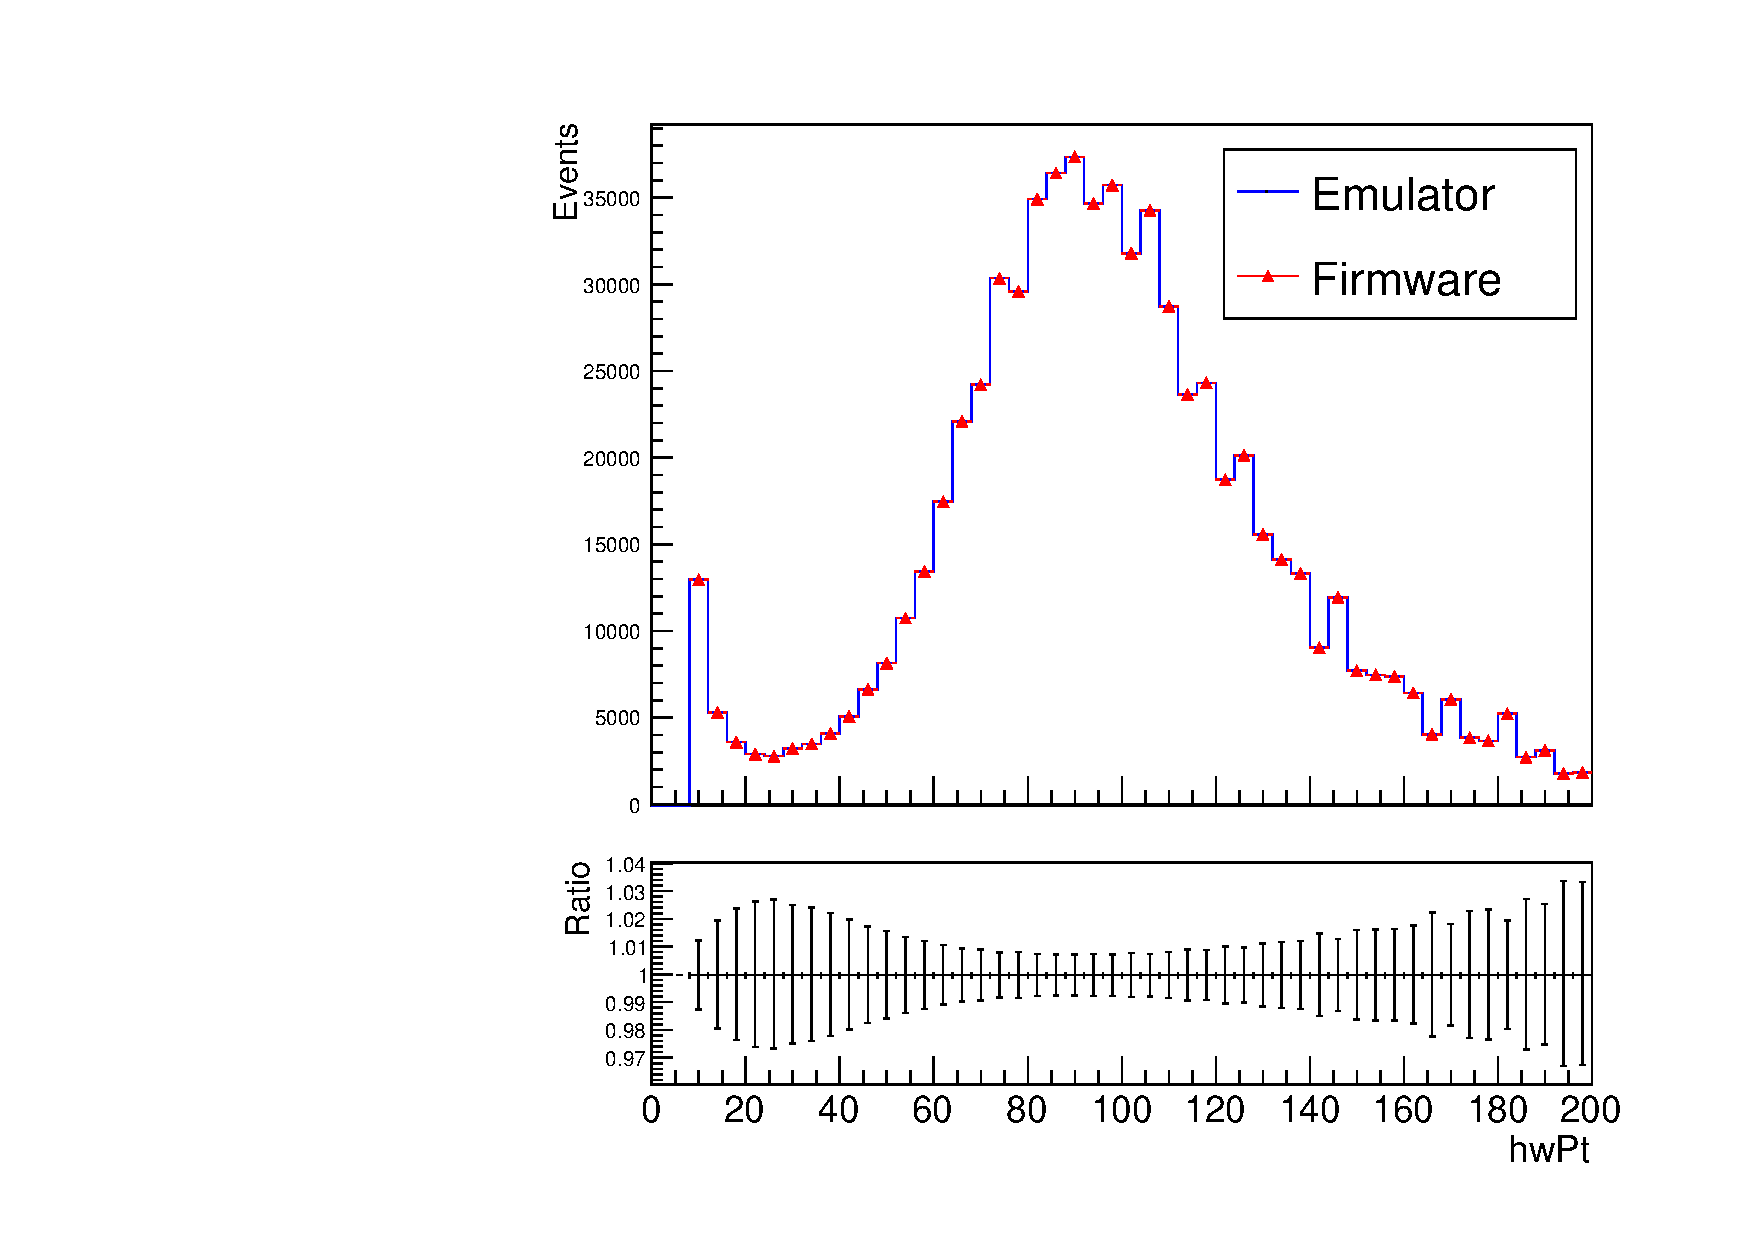
\includegraphics[width=0.55\linewidth]{figs/04_muons/emuVsFw_pt.pdf}
	\caption[Comparison of the track $p_T$ between the firmware and emulator using data from a 2017 Z tag-and-probe sample. hwPt represents the integer value of p$_T$ used in hardware. The emulator and firmware output show 100\% agreement across 500000 events.]{Comparison of the track $p_T$ between the firmware and emulator using data from a 2017 Z tag-and-probe sample. hwPt represents the integer value of p$_T$ used in hardware. The emulator and firmware output show 100\% agreement across 500000 events.}
	\label{fig:kmtf_fwVsEmu}
\end{figure}

\section{The Phase-2 KBMTF} \label{sec:HL_KBMTF}
The modifications to the KBMTF algorithm for the HL-LHC result from increased precision from the input trigger primitives and modifications to the trigger architecture. These changes mainly affect the firmware implementation and do not require conceptual changes to the logic used to propagate and update tracks. The propagation coefficients and Kalman Gain must be recalculated as the number of bits allocated to $k$, $\phi$, and $\phi_b$ change. Additionally, the firmware will receive primitives from the entire barrel muon system simultaneously as opposed to processing each wedge independently. The firmware will be time-multiplexed with a factor of 18, meaning data from each event will be sent to one of 18 processors running the KBMTF algorithm in parallel. Additionally, the FPGA will be changed to a ZYNQ Ultrascale+ and synthesized at a clock frequency of 200\unit{MHz}. Simulations show a resource utilization of 17\% LUT, 3\% FF, 11\% DSP, and 7\% BRAM~\cite{CERN-LHCC-2020-004}.

The KBMTF algorithm performance is robust to the high pileup conditions of the HL-LHC. The efficiencies remain the same as Phase-1, and the rate scales approximately linearly with pileup as expected. Figure~\ref{fig:rate_eff_HLLHC} shows the efficiency versus generated muon $p_T$, single muon rates versus threshold, and single muon rates versus pileup for the Phase-2 KBMTF and two proposed track finding algorithms. As discussed in section~\ref{sec:CMS_L1T}, the HL-LHC track trigger introduces new track primitives that will be used in novel muon triggers. These new algorithms have higher efficiency and precision for prompt muons due to the momentum resolution of the tracker, but will be unable to trigger on displaced muons as the track primitives do not include displaced tracks. 

\begin{figure} [htb!]
	\centering
	\captionsetup[subfigure]{justification=centering}
	\begin{subfigure}[h]{0.45\linewidth}
		\centering
		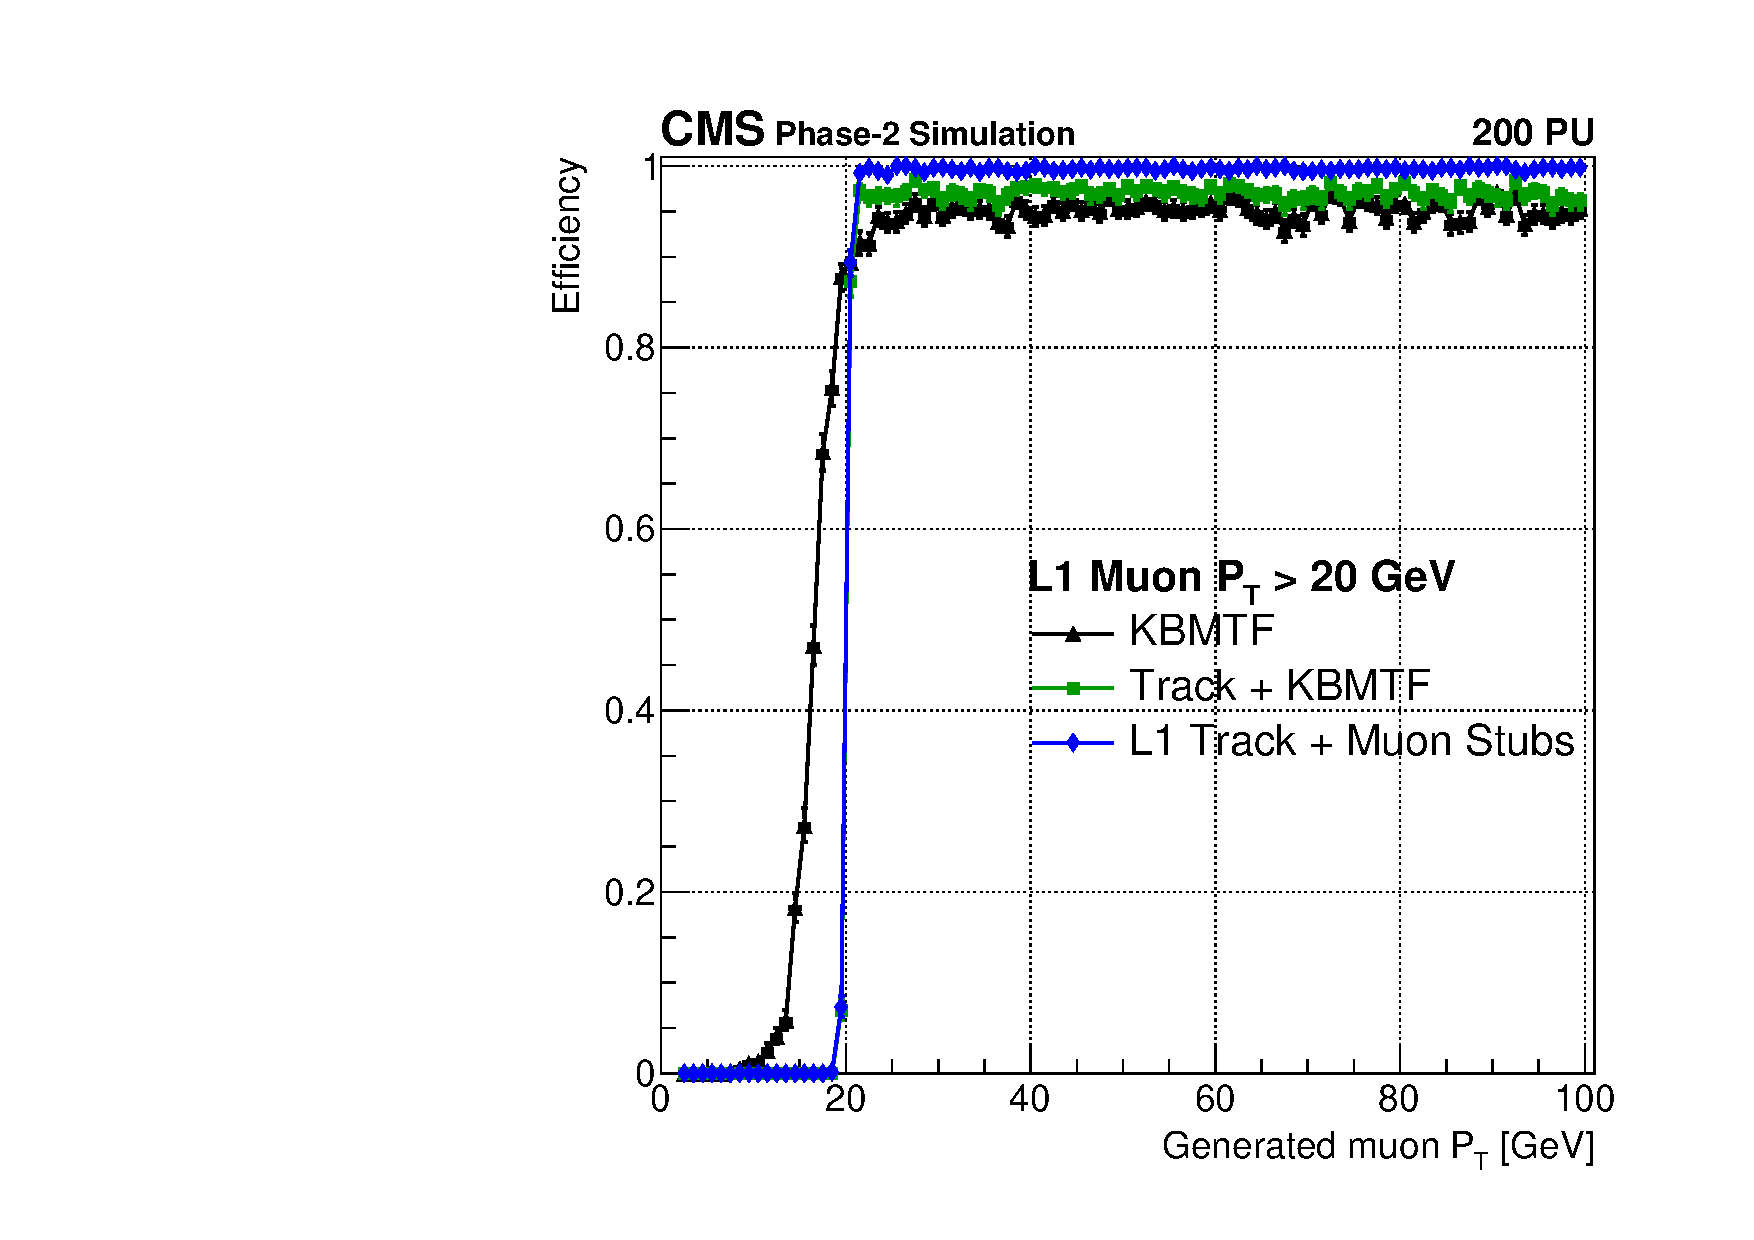
\includegraphics[width=\linewidth]{figs/04_muons/effVsPt_20_TPS.pdf}
		\caption{Efficiency vs gen $\mu$ $p_T$.}
		\label{}
	\end{subfigure} \hspace{0.05\linewidth}
	\begin{subfigure}[h]{0.45\linewidth}
		\centering
		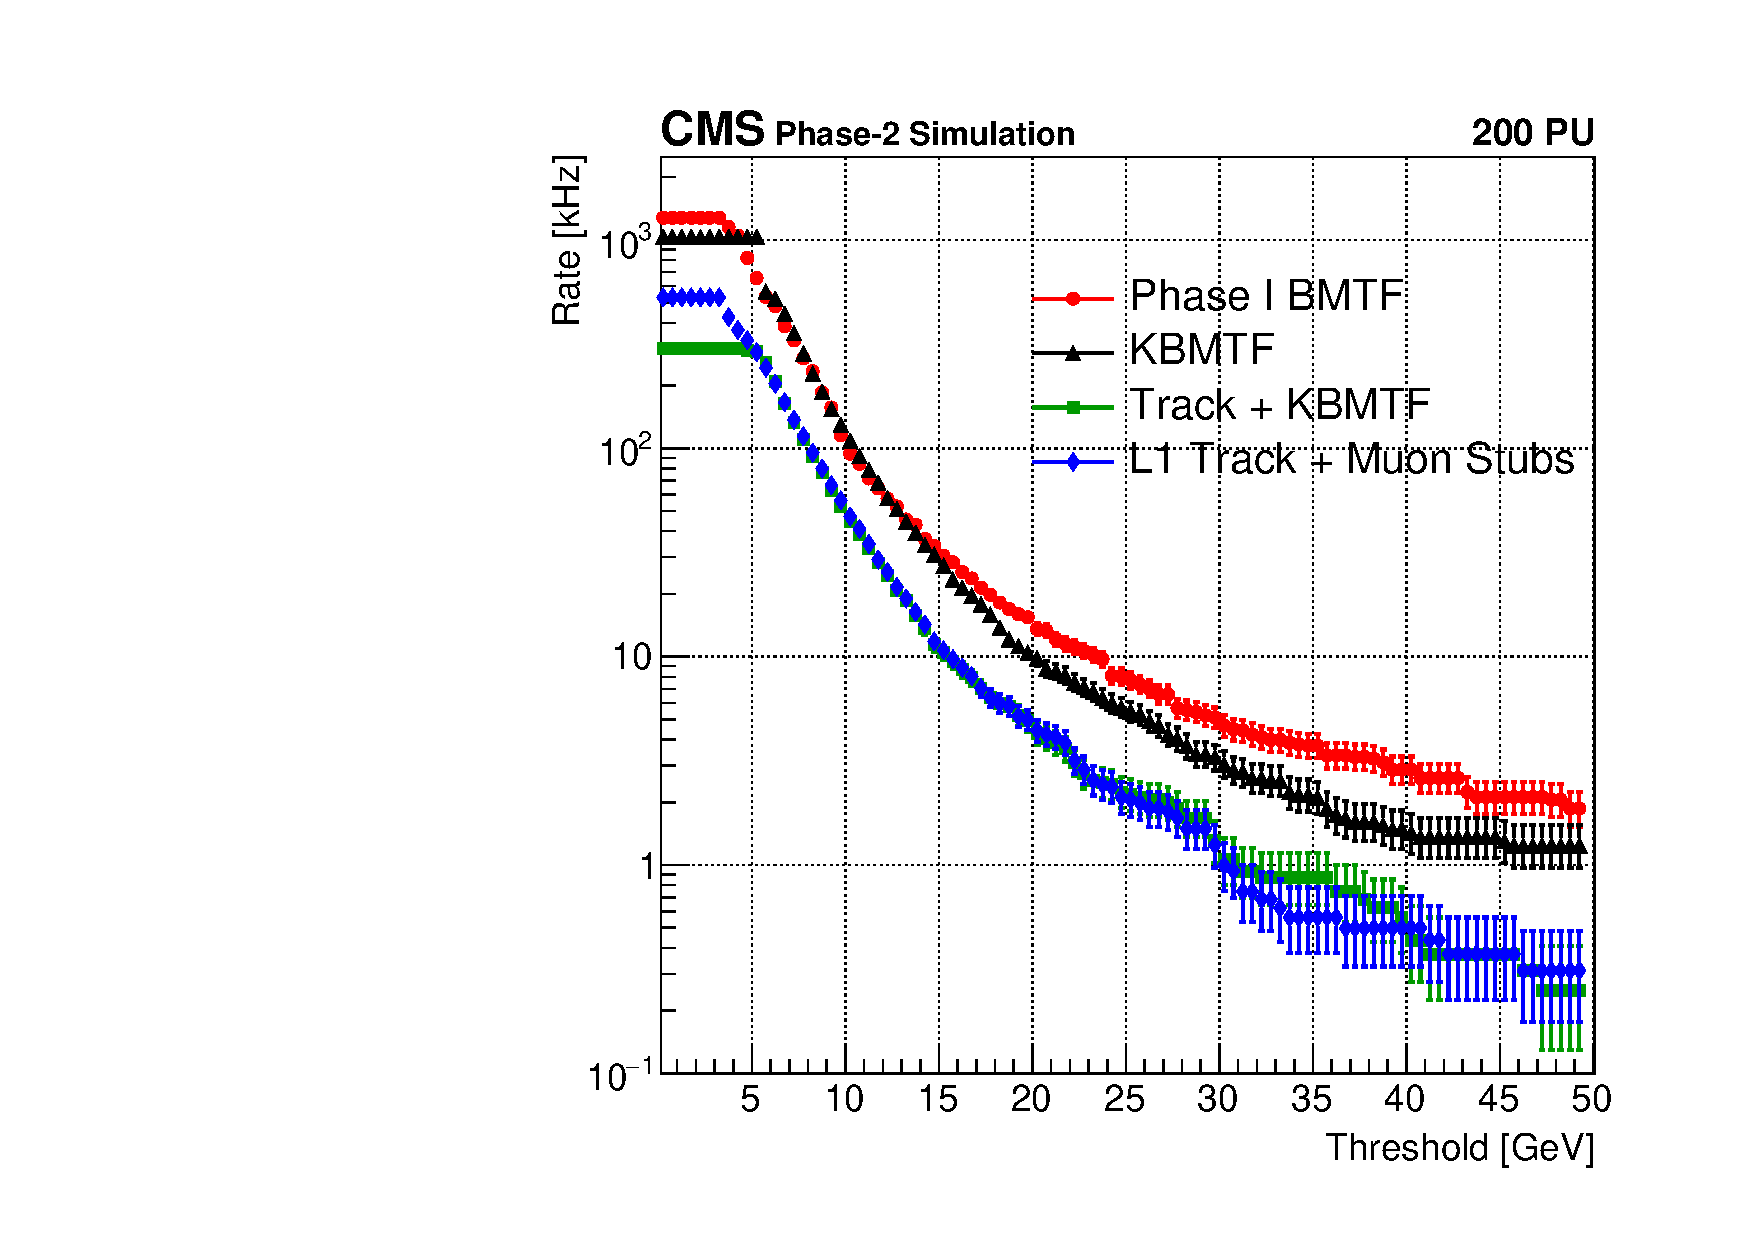
\includegraphics[width=\linewidth]{figs/04_muons/rateVsPt_TPS.pdf}
		\caption{Single muon rates versus threshold.}
		\label{}
	\end{subfigure}
	\begin{subfigure}[h]{0.45\linewidth}
		\centering
		\includegraphics[width=\linewidth]{figs/04_muons/rateVsPU_TPS.pdf}
		\caption{Single muon rates vs pileup for a 20\GeV threshold~\cite{CERN-LHCC-2020-004}}
		\label{}
	\end{subfigure}
	\caption[Performance of the L1 Barrel Muon algorithms using simulated samples with HL-LHC run conditions. The Track + KBMTF algorithm matches tracks to loose KBMTF muons, while the L1 Track + Muon Stubs algorithm matches tracks to muon stubs.]{Performance of the L1 Barrel Muon algorithms using simulated samples with HL-LHC run conditions. The Track + KBMTF algorithm matches tracks to loose KBMTF muons, while the L1 Track + Muon Stubs algorithm matches tracks to muon stubs.}
	\label{fig:rate_eff_HLLHC}
\end{figure}
% !TEX = root../thesis.tex

\chapter{Search for a Long Lived Scalar Boson}
\section{Introduction} \label{sec:ana_intro}
This chapter describes the search for rare Higgs boson decays to long lived scalar bosons ($\Phi$) decaying to a pair of photons using data taken by the CMS detector from 2016-2018. The following sections outline the choice of data sets and simulated samples, event selection criteria, methods of background estimation and statistical analysis for signal extraction, and results. This analysis is the first search for long lived photon pairs using a novel vertex reconstruction method to calculate the displaced vertex of the diphotons using kinematics.

The analysis is performed by searching for displaced diphoton decays of the Higgs bosons produced via associated production with a \PZ boson. Events are triggered and selected using the leptonic decays of the \PZ boson by requiring two high quality electrons or muons and two well reconstructed photons, with detailed criteria outlined in section~\ref{sec:ana_eventsel}. We utilize a data-driven background estimation shown in section~\ref{sec:ana_bkg} to model the background from Drell-Yan events containing photons from initial/final state radiation as well as neutral pions in jets, then extract the branching fraction of the Higgs boson to $\Phi\Phi$.

As described in section~\ref{sec:CMS_ECAL}, the CMS ECAL is a homogeneous calorimeter that measures the energy deposits from electromagnetically interacting particles. This lends the ECAL precise energy resolution but low capabilities to determine the direction particles were traveling when they reached the calorimeter, referred to as pointing. Photons are electrically neutral and do not leave tracks in the inner tracker, meaning that without pointing it is impossible to establish from where they originated. This places major restrictions searches for displaced photons, as the transverse distance traveled by the $\Phi$ before decaying to photons is the main variable used to extract the signal from data. We will show in section~\ref{sec:ana_vertex} that it is possible to recalculate the diphoton vertex using a kinematic constraint, which is performed for each hypothetical mass of the $\Phi$.

Results are calculated using a maximum likelihood based approach described in section~\ref{sec:ana_stats} to extract upper limits on the signal strength parameter. In section~\ref{sec:ana_res} we set limits on the product of the Higgs boson branching ratio to $\Phi\Phi$ times the LLP branching ratio to photons, as well as model independent limits on the generic \PZ + $\Phi\Phi$ cross section.

\section{Data and Simulated Samples} \label{sec:ana_samples}

\subsection{Data Samples} \label{sec:ana_data}
As discussed in chapter~\ref{chap:exp}, events that pass at least 1 HLT path are stored for future analysis. These events are collected and sorted into data sets based on the number and type of physics objects used in the HLT path. It can be noted that these data sets are not disjoint; one event can be sorted into multiple data sets if it satisfies more than a single HLT path, so care must be taken to avoid double counting events. The data are maintained and updated by the Physics Data and Monte Carlo Validation (PdmV) group, which also provides recommendations on optimal usage for physics analysis~\cite{pdmv}. This search utilizes the PdmV recommended data sets for Run-2 analyses, referred to as Ultra-Legacy (UL), which has been reprocessed using the most current calibration for detector responses and alignment. Although the characteristic signature of this analysis is two displaced photons, the HLT double photon triggers present in Run-2 are unsuitable for the phase space of signal photons. Therefore we utilize the leptonic decay of the associated \PZ which provides a robust trigger. Since we are interested in \PZ decays to either electrons or muons, we use the data sets labeled as SingleMuon or SingleElectron (renamed to EGamma in 2018). The complete list of data sets is listed in table~\ref{tab:datasets}.

\begin{table}[htb!]
	\centering
	\caption[CMS data sets used for each year in this analysis. Asterisks represents wildcards that cover the multiple data taking eras per year.]{CMS data sets used for each year in this analysis. Asterisks represents wildcards that cover the multiple data taking eras per year.}
	\label{tab:datasets}
	\begin{tabular}{l | l}
		\hline
		Year & CMS Data Set\\
		\hline
		\hline
		2018 & \small \begin{tabular}{>{\ttfamily}l}
			/EGamma/Run2018*-UL2018\_MiniAODv2\_NanoAODv9*\\
			/SingleMuon/Run2018*-UL2018\_MiniAODv2\_NanoAODv9*\\
			\end{tabular}\\
						\hline
		2017 & \small \begin{tabular}{>{\ttfamily}l}
				/SingleElectron/Run2017*-UL2017\_MiniAODv2\_NanoAODv9*\\
				/SingleMuon/Run2017-UL2017\_MiniAODv2\_NanoAODv9*\\
				\end{tabular}\\
							\hline
		2016 & \small \begin{tabular}{>{\ttfamily}l}
			/SingleElectron/Run2016*-UL2016\_MiniAODv2\_NanoAODv9*\\
			/SingleElectron/Run2016*\_HIPM\_UL2016\_MiniAODv2\_NanoAODv9*\\
			/SingleMuon/Run2016*-UL2016\_MiniAODv2\_NanoAODv9*\\
			/SingleMuon/Run2016*\_HIPM\_UL2016\_MiniAODv2\_NanoAODv9*\\
		\end{tabular}\\
	\hline
	\end{tabular}
\end{table}

The reprocessed datasets must be cross referenced with the "Golden JSON": a certificate created by the Data Quality Monitoring (DQM) group within CMS by monitoring each sub-detector system in order to veto collisions that occur during sub-optimal conditions. The total integrated luminosity recorded by CMS during Run-2 was $164\unit{fb^{-1}}$; however, only $138\unit{fb^{-1}}$ of that was certified for analysis. The total integrated luminosity and uncertainty per year for collisions recommended by DQM can be seen in table~\ref{tab:intLumi}.

\begin{table}[h]
	\centering
	\caption[Table of integrated luminosity per year~\cite{cmslumi2016,cmslumi2017,cmslumi2018}.]{Table of integrated luminosity per year~\cite{cmslumi2016,cmslumi2017,cmslumi2018}.}
	\label{tab:intLumi}
	\begin{tabular}{l|l|l|l|l}\hline
		Year & 2016 & 2017 & 2018 & 2016-2018\\
		\hline
		\hline
		Luminosity $[\text{fb}^{-1}]$ & 36.31 & 41.48 & 59.83 & 137.62\\
		\hline	
		Uncertainty $[\%]$ & 1.2 & 2.3 & 2.5 & 1.6\\
		\hline
	\end{tabular}
\end{table}

The 2016 data and simulation are divided into two distinct eras due to substantial changes to the silicon strip tracker. Saturation effects in the pre-amplifier of the APV25 readout chip resulted in a decreased signal-to-noise ratio and required a decrease to the feedback pre-amplifier bias voltage (referred to as VFP)~\cite{CMS-DP-2020-045}. As a result, simulated samples were produced separately for pre and post-VFP run conditions. The pre-VFP and post-VFP data corresponds to 19.65 and 16.67 \unit{fb^{-1}} respectively.

\subsection{Simulated Samples} \label{sec:ana_mc}
Simulated samples use Monte Carlo methods to generate events in several steps, from the matrix elements that determine cross sections for various physics processes, showering, and hadronization to detector responses and event reconstruction. These samples are generally created to model specific physics processes such as Drell-Yan, QCD, $t\bar{t}$, signal processes, etc. All samples used in this analysis use parton distribution functions given by NNPDF3.1~\cite{nnpdf3p1}. Simulated events are not created one-to-one to match data events; instead they are used to create weighted events that are normalized using the cross section of the simulated process and scaled to match the luminosity of the data. For this analysis we use both simulated background events as well as simulated signal samples.

\subsubsection{Monte Carlo Signal} \label{sec:ana_mcsig}
Standard Model Higgs production through quark induced and gluon induced \ZH processes are simulated at next-to-next-to leading order (NNLO) for several candidate mass points \mphi and lifetimes c$\tau$. The primary hard scattering interaction producing the Higgs Boson and associated \PZ boson is simulated with matrix elements calculated at NNLO using \textsc{Powheg box v2}~\cite{powheg}, while the subsequent decays of the Higgs Boson and showering processes are simulated using \textsc{Pythia8}~\cite{pythia8}. Leading order Feynman diagrams for the \ZH production are shown in figure~\ref{fig:ZH_feynman}, while the decays of the $\Phi$ boson can be seen in figure~\ref{fig:htophiphi}. The parameters for Pythia8 simulations were set to TuneCP5, which were the optimal values for agreement with measured data at NNLO at the time of producing the samples~\cite{tunecp5}. The simulated signal samples were produced centrally by the Monte Carlo and Interpretation subgroup of CMS.

\begin{figure}[htb!]
	\centering
	\begingroup
	\tikzset{every picture/.style={scale=0.5}}
	\hfill
	% !TEX = root = ../../thesis.tex
\begin{tikzpicture}
	\begin{feynman}
		% Defining vertex coordinates
		\coordinate[label=left:$q$] (i1) at (-3.5, 2); %Initial q
		\coordinate[label=left:$\bar{q}$] (i2) at (-3.5,-2); %Initial qbar
		\coordinate (v1) at (-1.5, 0); %vertex 1
		\coordinate (v2) at (1.5, 0);  %vertex 2
		\coordinate[label=right:$H$] (f1) at (3.5, 2);  %Higgs
		\coordinate[label=right:$Z$] (f2) at (3.5, -2); %Z

		% Drawing everything
		\draw[fermion] (i1) -- (v1);
		\draw[fermion] (v1) -- (i2);
		\draw[boson] (v1) -- (v2);
		\draw[boson] (f2) -- (v2);
		\draw[scalar] (v2) -- (f1);
		
		\node[label={below:$Z$}] at (0, 0){};
	\end{feynman}
\end{tikzpicture}
	\hfill
	% !TEX = root = ../../thesis.tex
\begin{tikzpicture}
	\begin{feynman}
		% Defining vertex coordinates
		\coordinate[label=left:$g$] (g1) at (-4, 2.5); % initial g
		\coordinate[label=left:$g$] (g2) at (-4, -2.5); % Initial g
		\coordinate (q1) at (-3, 1); %Initial q
		\coordinate (q2) at (-3,-1); %Initial qbar
		\coordinate (v1) at (-1.5, 0); %vertex 1
		\coordinate (v2) at (1.5, 0);  %vertex 2
		\coordinate[label=right:$H$] (f1) at (3.5, 2);  %Higgs
		\coordinate[label=right:$Z$] (f2) at (3.5, -2); %Z
		
		% Drawing everything
		\draw[gluon] (g1) -- (q1);
		\draw[gluon] (g2) -- (q2);
		\draw[fermion] (q1) -- (v1);
		\draw[fermion] (v1) -- (q2);
		\draw[fermion] (q2) -- (q1);
		\draw[boson] (v1) -- (v2);
		\draw[boson] (f2) -- (v2);
		\draw[scalar] (v2) -- (f1);
			
		\node[label={below:$Z$}] at (0, 0){};
	\end{feynman}
\end{tikzpicture}
	\hfill
	% !TEX = root = ../../thesis.tex
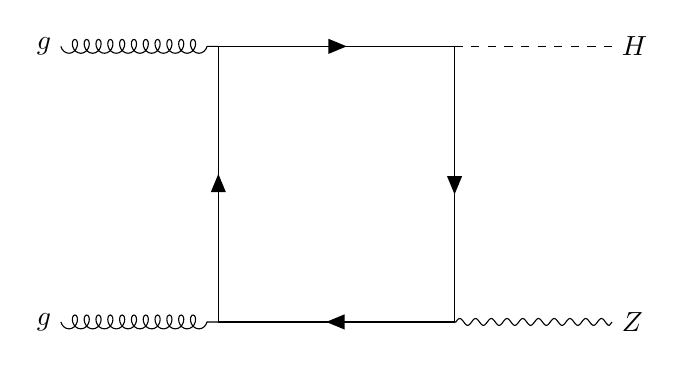
\begin{tikzpicture}
	\begin{feynman}
		% Defining vertex coordinates
		\coordinate[label=left:$g$] (g1) at (-3.5, 1.75); % initial g
		\coordinate[label=left:$g$] (g2) at (-3.5, -1.75); % Initial g
		\coordinate (q1) at (-1.5, 1.75);
		\coordinate (q2) at (1.5, 1.75); 
		\coordinate (q3) at (1.5,-1.75);
		\coordinate (q4) at (-1.5, -1.75);
		\coordinate[label=right:$H$] (f1) at (3.5, 1.75);  %Higgs
		\coordinate[label=right:$Z$] (f2) at (3.5, -1.75); %Z
		
		% Drawing everything
		\draw[gluon] (g1) -- (q1);
		\draw[gluon] (g2) -- (q4);
		\draw[fermion] (q1) -- (q2);
		\draw[fermion] (q2) -- (q3);
		\draw[fermion] (q3) -- (q4);
		\draw[fermion] (q4) -- (q1);
		\draw[boson] (q3) -- (f2);
		\draw[scalar] (q2) -- (f1);
	
	\end{feynman}
\end{tikzpicture}
	\hfill
	\endgroup
	\caption[Feynman diagrams for both quark induced and gluon induced \PZns+\PH production.]{Feynman diagrams for both quark induced and gluon induced \PZns+\PH production.}
	\label{fig:ZH_feynman}
\end{figure}

The Higgs Boson is forced to decay to two long lived scalar bosons ($\Phi$). Each $\Phi$ has a 50\% branching ratio to $\gamma\gamma$ and a 50\% branching ratio to $d\bar{d}$ as shown in figure~\ref{fig:htophiphi}. The decay to $d\bar{d}$ was chosen to create a generic jet with no characteristic signature that would affect the event topology. Additional samples with a 100\% branching ratio to $\gamma\gamma$ were generated to provide better statistical power for four photon decays. The \PZ is forced to decay leptonically, which is accounted for when normalizing samples for the limit setting procedure. A complete list of masses, lifetimes, and number of generated events is shown in table~\ref{tab:sigsamples}.

\begin{figure}[htb!]
	\centering
	% !TEX = root = ../../thesis.tex
\begin{tikzpicture}
	\begin{feynman}
		% Defining vertex coordinates
		\coordinate[label=left:$H$] (h1) at (-2.5, 0); %Initial Higgs
		\coordinate (v1) at (0, 0); %First vertex
		\coordinate (phi1) at (2, 1.25); %Phi 1
		\coordinate (phi2) at (2, -1.25); %Phi 2
		\coordinate (q1) at (3.25, 2.); %q1
		\coordinate (q2) at (3.25, .75); %q2
		\coordinate[label=right:$\gamma$] (g1) at (4.5, 2);
		\coordinate[label=right:$\gamma$] (g2) at (4.5, .75);
		\coordinate[label=right:$d$] (d1) at (3.5, -.5);
		\coordinate[label=right:$\bar{d}$] (d2) at (3.5, -2);

		\draw[scalar] (h1) -- (v1);
		\draw[scalar] (v1) -- (phi1);
		\draw[scalar] (v1) -- (phi2);
		\draw[fermion] (phi1) -- (q1);
		\draw[fermion] (q1) -- (q2);
		\draw[fermion] (q2) -- (phi1);
		\draw[photon] (q1) -- (g1);
		\draw[photon] (q2) -- (g2);
		\draw[fermion] (phi2) -- (d1);
		\draw[fermion] (d2) -- (phi2);
		
		\node[label={above,left:$\Phi$}] at (1, .75){};
		\node[label={below,left:$\Phi$}] at (1, -.75){};
		\node[label={left:$\textbf{?}$}] at (3.325, 1.375){};
	\end{feynman}
\end{tikzpicture}
	\caption[Feynman diagram showing the proposed decay channel of the Higgs boson to $\Phi\Phi$, with one $\Phi$ decaying to a pair of photons and the other decaying to $d\bar{d}$. The loop in the diphoton decay can contain any particle that could theoretically couple to the $\Phi$. It is also possible for the $\Phi$ to decay directly to photons.]{Feynman diagram showing the proposed decay channel of the Higgs boson to $\Phi\Phi$, with one $\Phi$ decaying to a pair of photons and the other decaying to $d\bar{d}$. The loop in the diphoton decay can contain any particle that could theoretically couple to the $\Phi$. It is also possible for the $\Phi$ to decay directly to photons.}
	\label{fig:htophiphi}
\end{figure}

\begin{table}[htb!]
	\caption[Mass points, lifetimes, and number of simulated H $\rightarrow \Phi\Phi$ events for the 2$\gamma$2q categories. Number of events generated is halved for the 4$\gamma$ categories]{Mass points, lifetimes, and number of simulated H $\rightarrow \Phi\Phi$ events for the 2$\gamma$2q categories. Number of events generated is halved for the 4$\gamma$ categories}
	\label{tab:sigsamples}
	\begin{center}
		\begin{tabular}{l|l|l}
			\hline
			m$_\Phi$ [GeV] & c$\tau$ [mm] &  Events\\
			\hline
			15 & 0, 10, 20, 50, 100, 1000 & 100000\\
			\hline
			20, 30, 40, 50, 55 & 0, 10, 20, 50, 100 & 50000\\
			& 1000 & 100000\\
			\hline
		\end{tabular}
	\end{center}
\end{table}

\subsubsection{Signal Lifetime Reweighting} \label{sec:ana_ctau}
One can interpolate between signal sample lifetimes using a process known as c$\tau$ reweighting. As each generated event contains two $\Phi$ with exponentially distributed lifetimes, an event weight can be applied to generated a sample of arbitrary lifetime. Assume an event generated with mean lifetime $\tau_0$, with each $\Phi$ lifetime given by $t_1$ and $t_2$. To reweight this sample to a new mean lifetime $\tau_\mathrm{new}$, we apply a weight given by the ratio of poisson probability distributions
\begin{equation}\label{eq:ctreweight}
	w(\tau_0, \tau_{\mathrm{new}}, t_1, t_2) =\frac{\mathcal{P}(t_1|\tau_\mathrm{new})\mathcal{P}(t_2|\tau_\mathrm{new})}{\mathcal{P}(t_1|\tau_0)\mathcal{P}(t_2|\tau_0)}= \left(\frac{\tau_0}{\tau_{\mathrm{new}}}\right)^2 \frac{e^{\frac{-(t_2+t_1)}{\tau_{\mathrm{new}}}}}{e^{\frac{-(t_2+t_1)}{\tau_0}}}
\end{equation}
The $\Phi$ lifetimes $t_i$ can be calculated from the generator level information as follows
\begin{equation} \label{eq:lifetime}
	ct=\frac{\beta}{\gamma}\cdot\mathrm{ip}_{\mathrm{3D}}=\frac{m|\mathbf{p}|}{E^2}\cdot\mathrm{ip}_\mathrm{3D}
\end{equation}
Where $c$ is the speed of light, $m$, $\mathbf{p}$, and $E$ are the mass, 3-momentum, and energy of the $\Phi$ and the three-dimensional impact parameter $\mathrm{ip}_\mathrm{3D}$ is the distance in the lab frame traveled by the $\Phi$ from the PV before decaying. 

Lifetimes are reweighted to 3, 14, 32, 70, and 316\unit{mm} to be uniformly distributed between generated signal samples on a logarithmic scale. The signal sample with the nominal lifetime closest to the target lifetime is chosen to be reweighted, excluding the 3\unit{mm} sample which is produced using the 10\unit{mm} sample.

\subsubsection{Pileup Reweighting} \label{sec:ana_pu}
Events passing the HLT generally consist of one interesting hard-scatter occurring at the primary vertex (PV). However, as discussed in chapter~\ref{sec:CMS_trig}, colliding proton bunches often produces secondary collisions along the beamline known as pileup (PU). Particles resulting from PU are generally uninteresting on their own but produce tracks and energy deposits that affect event reconstruction. During Run-2 data taking the average pileup ranged from 27 in 2016 to 37 in 2018. PU distributions in data can be seen in figure~\ref{fig:pileup}.

\begin{figure}[htb!]
	\centering
	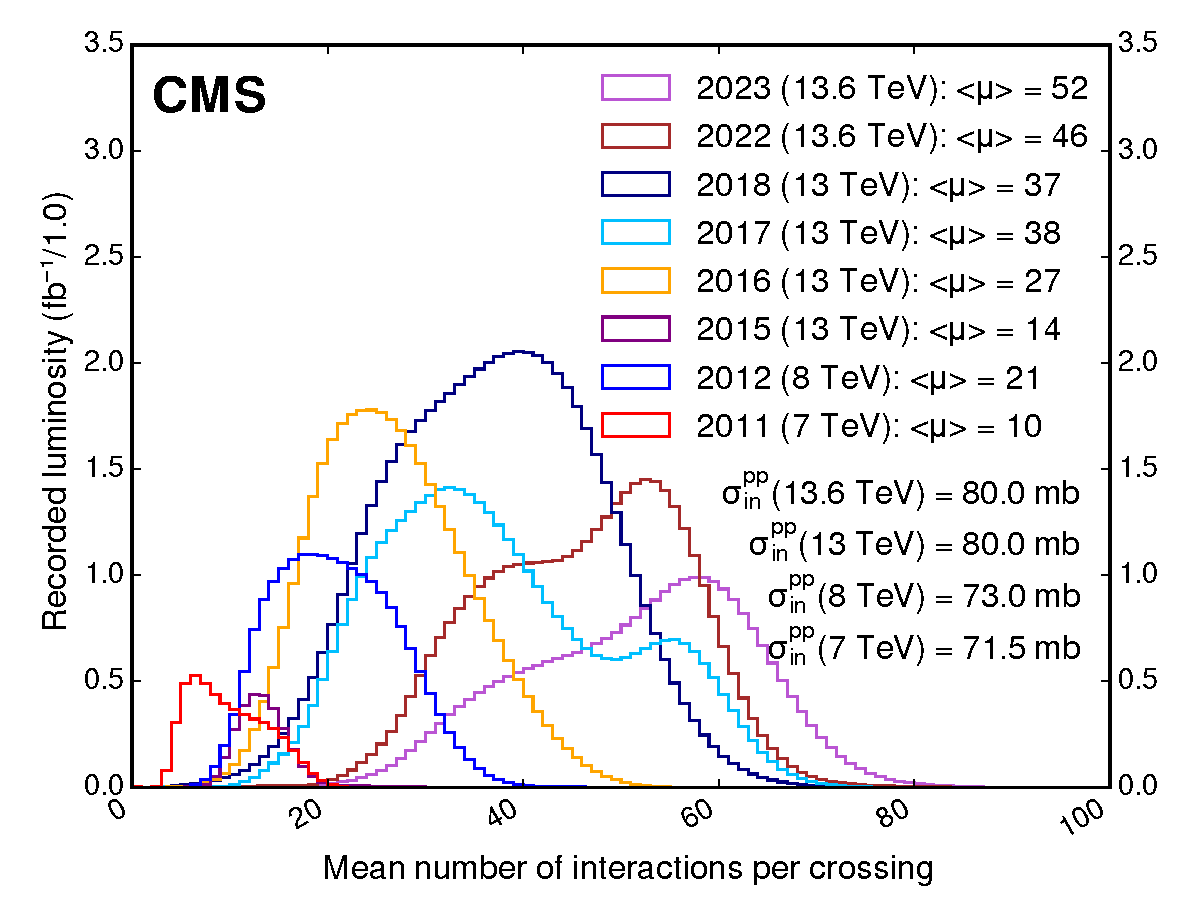
\includegraphics[width=0.8\linewidth]{figs/05_analysis/pileup_allYears.pdf}
	\caption[Pileup distributions and mean PU from 2011-2023 datataking~\cite{CMSlumi}.]{Pileup distributions and mean PU from 2011-2023 datataking~\cite{CMSlumi}.}
	\label{fig:pileup}
\end{figure}

Monte Carlo samples account for secondary collisions by generating PU interactions according to a predetermined distribution. However, the distribution of the number of interactions does not exactly match what is observed in data. To account for this, we apply a weight to simulated samples as a function of the number of simulated PU interactions by dividing a histogram of data PU distributions by the Monte Carlo PU distribution.

\subsubsection{Monte Carlo Background} \label{sec:ana_mcbkg}
Although this analysis employs a data driven method of background estimation, simulated samples are used to inform on properties of background events and tune cuts to discriminate between signal and background. For this analysis, we use simulated Drell-Yan (DY) to $\ell\ell$ events with 0, 1 and 2 additional jets, simulated using matrix elements calculated at NNLO. Studies were done with inclusive (any number of additional jets) samples but found these samples to have worse agreement in control regions and statistical power compared to the jet categorized samples. The cross sections used for normalization were calculated using the \texttt{GenXSecAnalyzer}, a tool provided by CMS to calculate the cross sections for simulated samples~\cite{genxsecana}. A list of cross sections for each simulated process can be found in table~\ref{tab:mcsamples}.

\begin{table}[htb!]
	\centering
	\caption[List of simulated background processes, their cross sections calculated using \texttt{GenXSecAnalyzer}~\cite{genxsecana}, and CMS data set names.]
	{List of simulated background processes, their cross sections calculated using \texttt{GenXSecAnalyzer}~\cite{genxsecana}, and CMS data set names. Asterisks stand for \texttt{18NanoAODv9-106X\_upgrade2018\_realistic\_v16} for 2018, \texttt{17NanoAODv9-106X\_mc2017\_realistic} for 2017, \texttt{6NanoAODAPVv9-106X\_mcRun2\_asymptotic\_preVFP} for 2016 pre-VFP, and \texttt{16NanoAODv9-106X\_mcRun2\_asymptotic} for 2016 post-VFP.}
	\label{tab:mcsamples}
	\begin{tabular}{l c l}\hline
		Process & Cross Section [pb] & Data set\\
		\hline
		DY + 0 jets & 5090 & \scriptsize\texttt{DYJetsToLL\_0J\_TuneCP5\_13TeV-amcatnloFXFX-pythia8/RunIISummer20UL*}\\
		DY + 1 jet & 983.5 & \scriptsize\texttt{DYJetsToLL\_1J\_TuneCP5\_13TeV-amcatnloFXFX-pythia8/RunIISummer20UL*}\\
		DY + 2 jets & 353.5 & \scriptsize\texttt{DYJetsToLL\_2J\_TuneCP5\_13TeV-amcatnloFXFX-pythia8/RunIISummer20UL*}\\
		\hline
	\end{tabular}
	
\end{table}

\subsubsection{Scale Factor Corrections} \label{sec:ana_sf}
Scale factors are corrective weights applied to simulated events in order to improve the agreement to data. The total weight applied is defined by the data-to-simulation efficiency ratio, given by
\begin{equation}
	S=\frac{\epsilon(\text{data})}{\epsilon(\text{MC})}
\end{equation}
The total efficiency $\epsilon$ in data and Monte Carlo is a product of the efficiencies for each object used in the event selection. The efficiency for a given object is itself a product of several individual efficiencies. For muons, the efficiency $\epsilon_\mu=\epsilon_\text{reco}\times\epsilon_\text{trig}\times\epsilon_\text{ID}\times\epsilon_\text{iso}$ is a product of the muon track reconstruction efficiency, trigger efficiency, ID efficiency, and isolation efficiency. For electrons and photons, $\epsilon_\text{iso}$ is absorbed into the $\epsilon_\text{ID}$ efficiency because the cut based ID includes the isolation. The efficiency for electrons is then $\epsilon_e=\epsilon_\text{reco}\times\epsilon_\text{trig}\times\epsilon_\text{ID}$. Photons are not used for any HLT triggers nor do they have associated tracks, so $\epsilon_\text{trig}$ and $\epsilon_\text{reco}$ are omitted, making the total efficiency $\epsilon_\gamma=\epsilon_\text{pix}\times\epsilon_\text{ID}$, where $\epsilon_\text{pix}$ is the efficiency for the pixel seed veto. The total scale factor is then given by
\begin{equation}
	S=\prod_{i\in\mu,e,\gamma}\frac{\epsilon_i(\text{data})}{\epsilon_i(\text{MC})}
\end{equation}
All scale factors are centrally measured and provided by the respective POGs with the exception of the electron trigger efficiencies, which were privately produced. Almost all efficiencies are measured with the tag-and-probe technique, which uses events containing one lepton passing strict selection criteria (the "tag") and one oppositely charged same flavor lepton passing loose selection criteria (the "probe"), where the dilepton invariant mass lies within the \PZ resonance centered at $91\GeV$. The strict tag and invariant mass criteria give a set of real leptons that are unbiased due to the loose probe criteria which are used to calculate various efficiencies. This method was adapted for photon ID efficiency calculations by ignoring the tracker information for $\PZ\to ee$ events and treating the calorimeter clusters as photons. The photon pixel seed veto efficiencies require tracker information and cannot be calculated using $\PZ\to ee$ tag-and-probe techniques. These were instead measured using $\PZ\to\mu\mu+\gamma$ events, where the photon is from final state radiation. Invariant mass and topological cuts give a clean sample of unbiased photons which are used to calculate $\epsilon_\text{pix}$.

Electron HLT scale factors were not centrally provided and were calculated privately using the tag-and-probe technique described above. The tag+probe were required to have a combined invariant mass of $60<m_\text{tag-probe}<125\GeV$. Baseline criteria for the tag and probe can be seen in table~\ref{tab:tnp}.
\begin{table} [htb!]
	\centering
	\caption{Tag and probe criteria used to derive HLT scale factors}
	\label{tab:tnp}
	\begin{tabular}{l | l}
		\hline
		Tag Criteria & Probe Criteria \\
		\hline
		\hline
		\begin{tabular}{l}
			Matched to Single Electron Trigger\\
			Passing tight cut-based ID\\
			$|\eta| < 2.17$\\
			$|\eta| < 1.4442$ or $|\eta| > 1.566$\\
			$\pt > 35\GeV$\\
		\end{tabular}  & 
		\begin{tabular}{l}
			$\pt > 15\GeV$\\
			$|\eta| < 2.5$\\
			$E_{T} > 5\GeV$\\
			$|d_{z}| < 0.2\unit{cm}$ \\
			$|d_{xy}| < 0.2\unit{cm}$\\
			Passes tight cut-based ID\\
		\end{tabular} \\
		\hline
	\end{tabular}
\end{table}

Events that pass the baseline tag/probe criteria are binned according to the \pt and $\eta_{sc}$ of the probe, and split into pass/fail histograms if the probe passed/failed to trigger the HLT path. For data, the histograms are fit analytically using the \PZ peak plus background to extract the number of signal events and calculate the efficiency. In Monte Carlo, the events are first matched to generator level electrons originating from the \PZ to ensure zero background events and fit to only the \PZ signal. The signal is modeled using a piecewise function with the upper and lower sides modeled using gaussian cores and exponential tails, which is then convolved with the world-average \PZ mass and width~\cite{Sirunyan_2021}. Background is modeled by multiplying an error function with a falling exponential. To calculate the systematic uncertainty of the fit, the efficiencies are calculated for data under alternative signal and background models. For the alternate signal, the data models the signal shape as a convolution of a gaussian and the Monte Carlo signal from the equivalent bin. For the alternate background, the shape is modeled as just an exponential, which can either grow or decay depending on the \pt and $\eta$ range of the bin. This process is repeated for each era, as the trigger and run conditions can vary between years. The trigger efficiency as a function of $\eta$ can be seen in figure~\ref{fig:effVsEta_electronHLT}. A full set of scale factors is shown in figures~\ref{fig:UL2018_SF2D} - \ref{fig:UL2016_preVFP_SF2D}.

\begin{figure}[htb!]
	\centering
	\captionsetup[subfigure]{justification=centering}
	\begin{subfigure}[h]{0.45\linewidth}
		\centering
		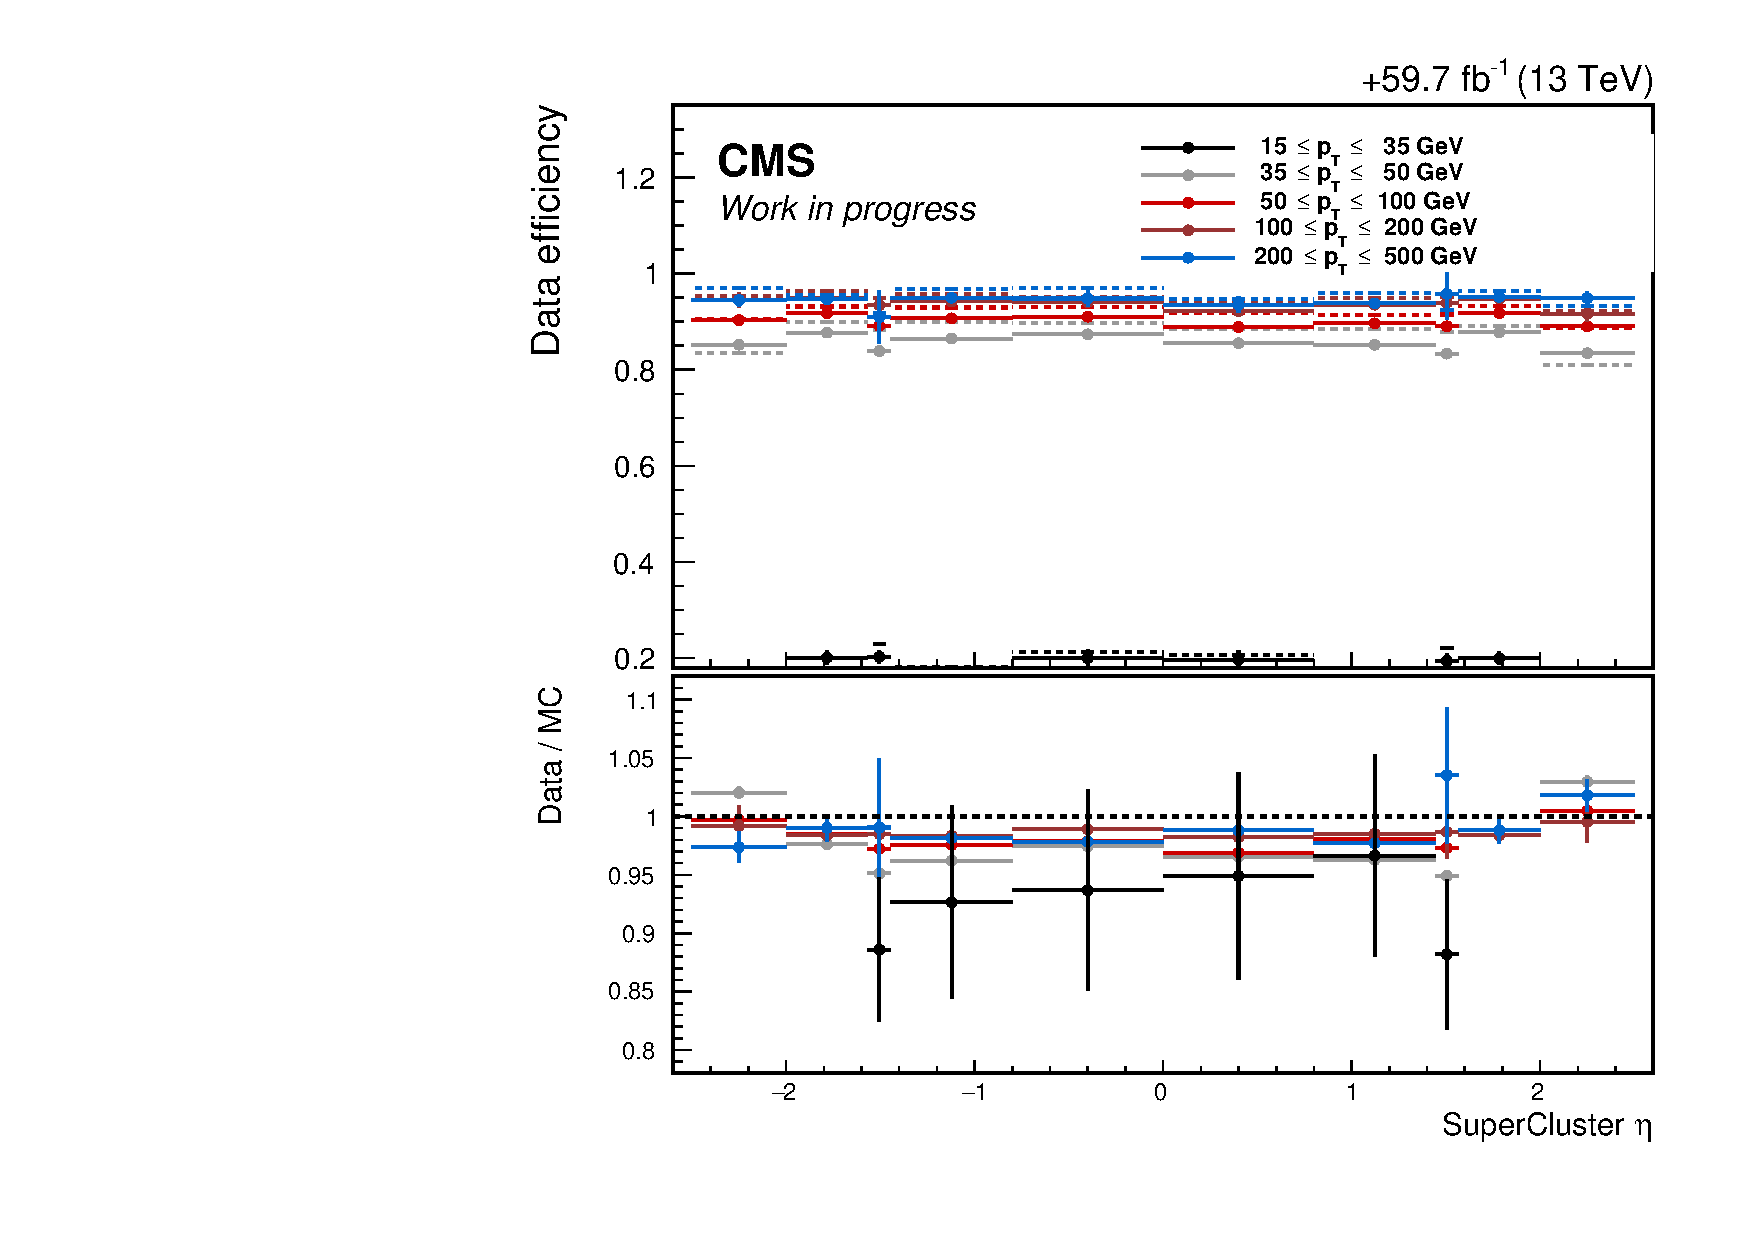
\includegraphics[width=\linewidth]{figs/05_analysis/UL2018_SFvseta_myWP.pdf}
		\caption{2018}
	\end{subfigure}
	\begin{subfigure}[h]{0.45\linewidth}
		\centering
		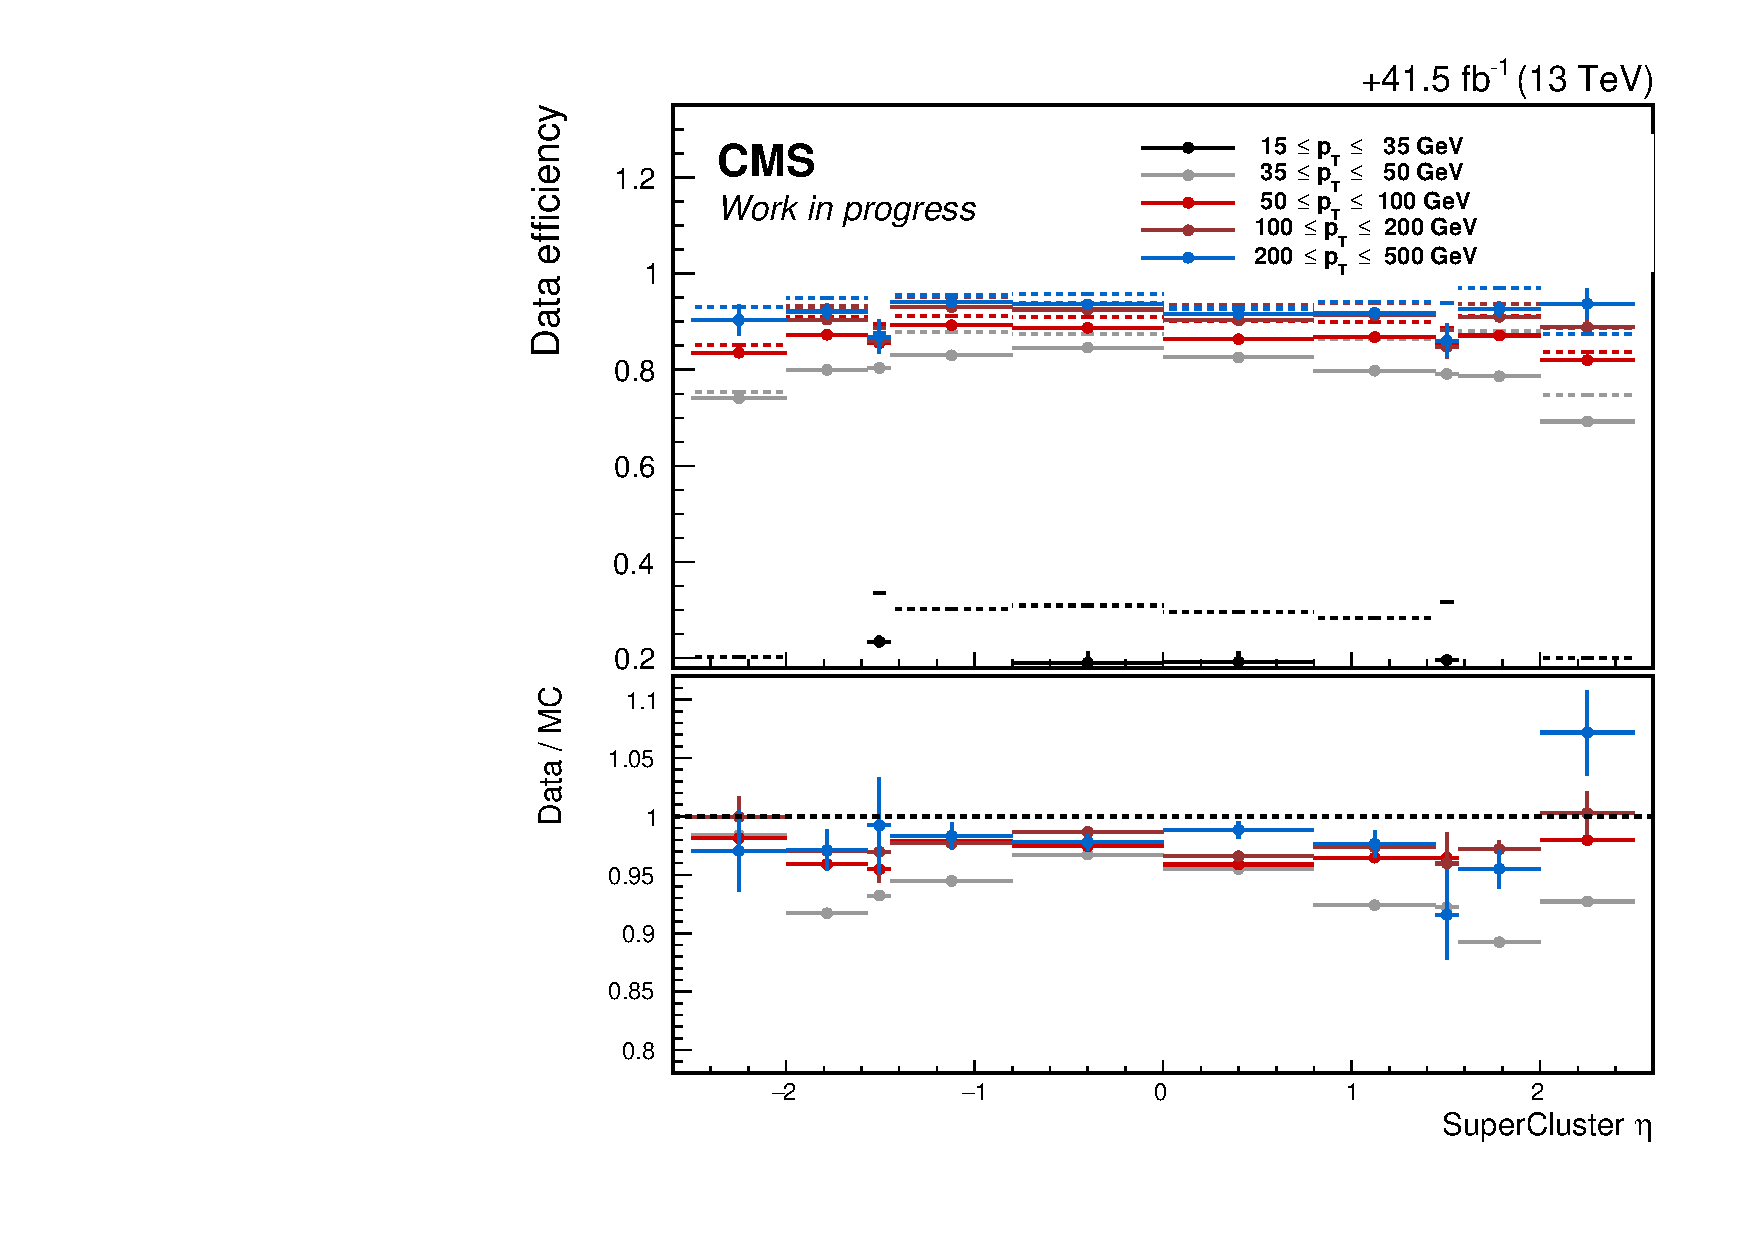
\includegraphics[width=\linewidth]{figs/05_analysis/UL2017_SFvseta_myWP.pdf}
		\caption{2017}
	\end{subfigure}
	\begin{subfigure}[h]{0.45\linewidth}
		\centering
		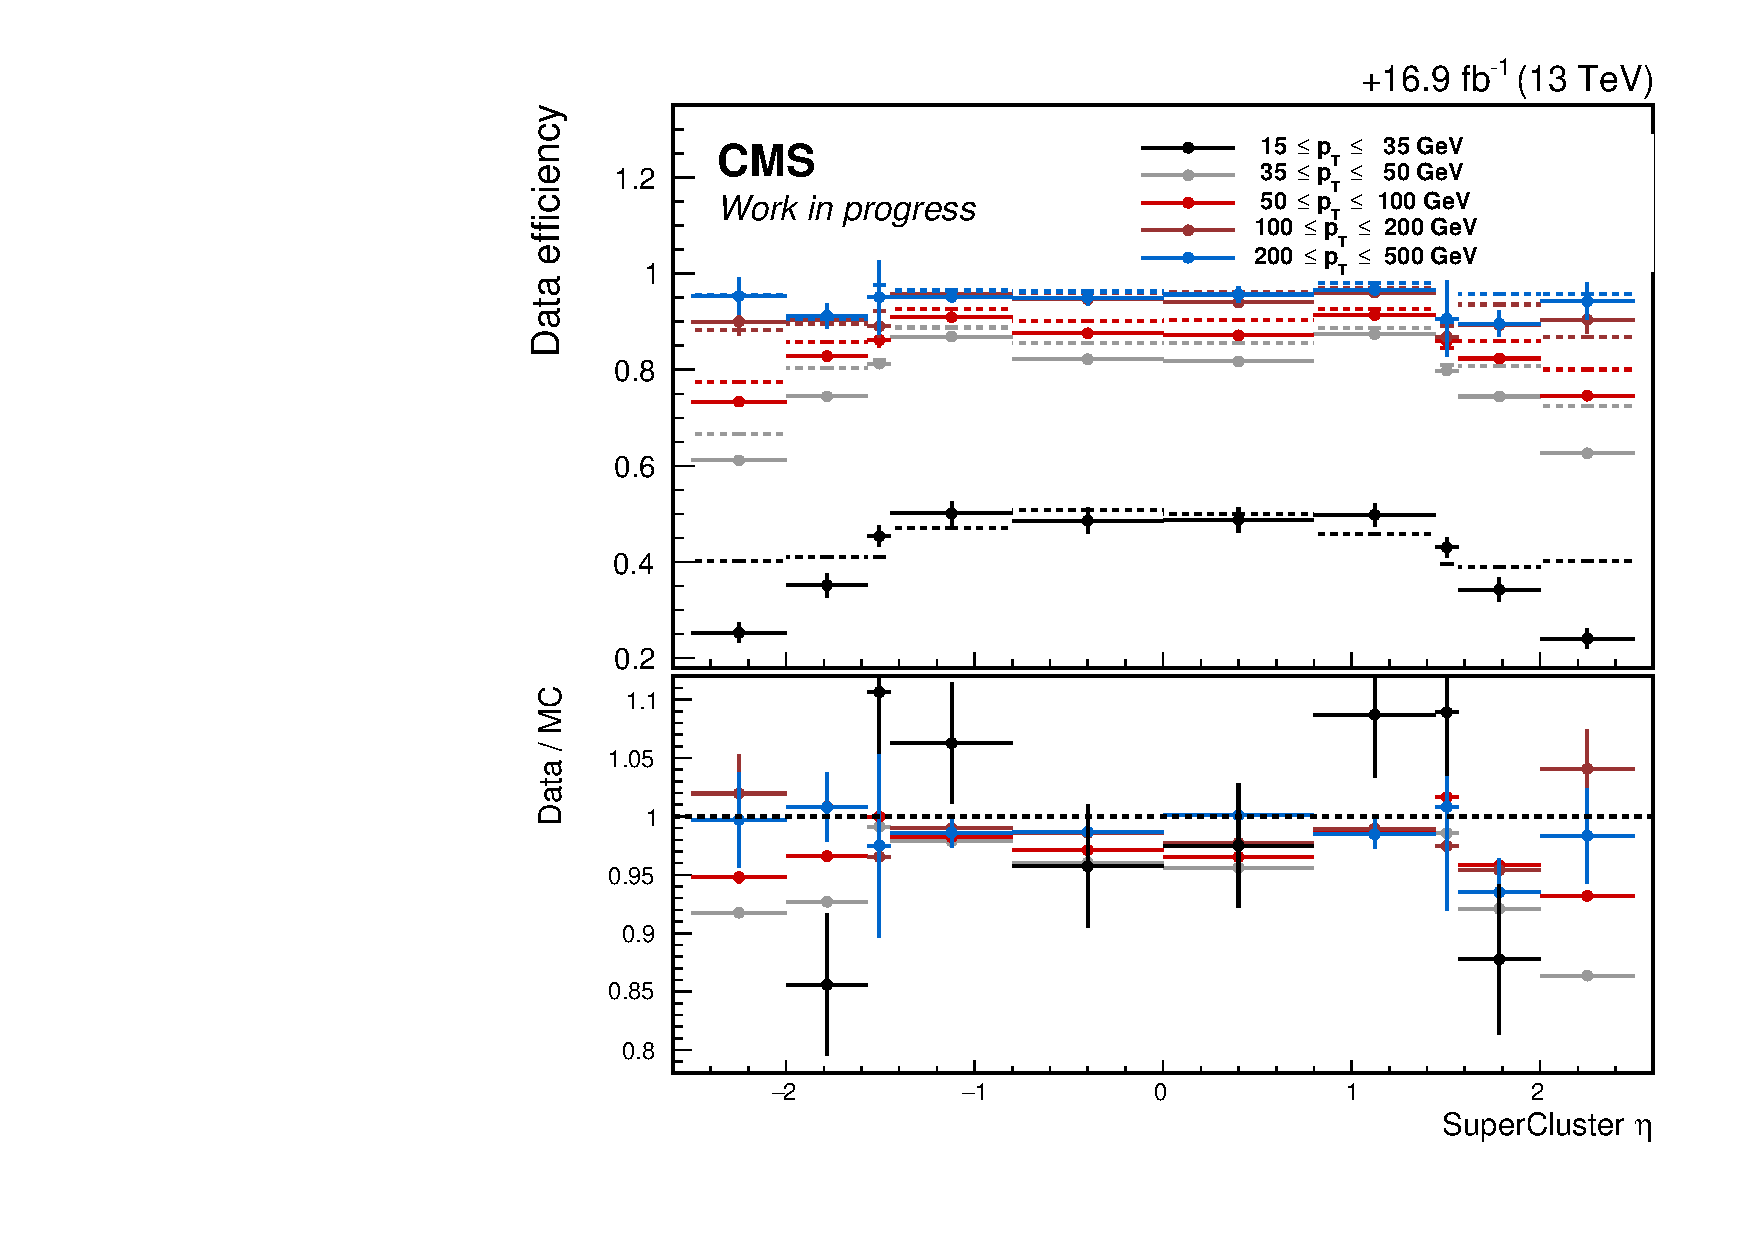
\includegraphics[width=\linewidth]{figs/05_analysis/UL2016_postVFP_SFvseta_myWP.pdf}
		\caption{2016 post-VFP}
	\end{subfigure}
	\begin{subfigure}[h]{0.45\linewidth}
		\centering
		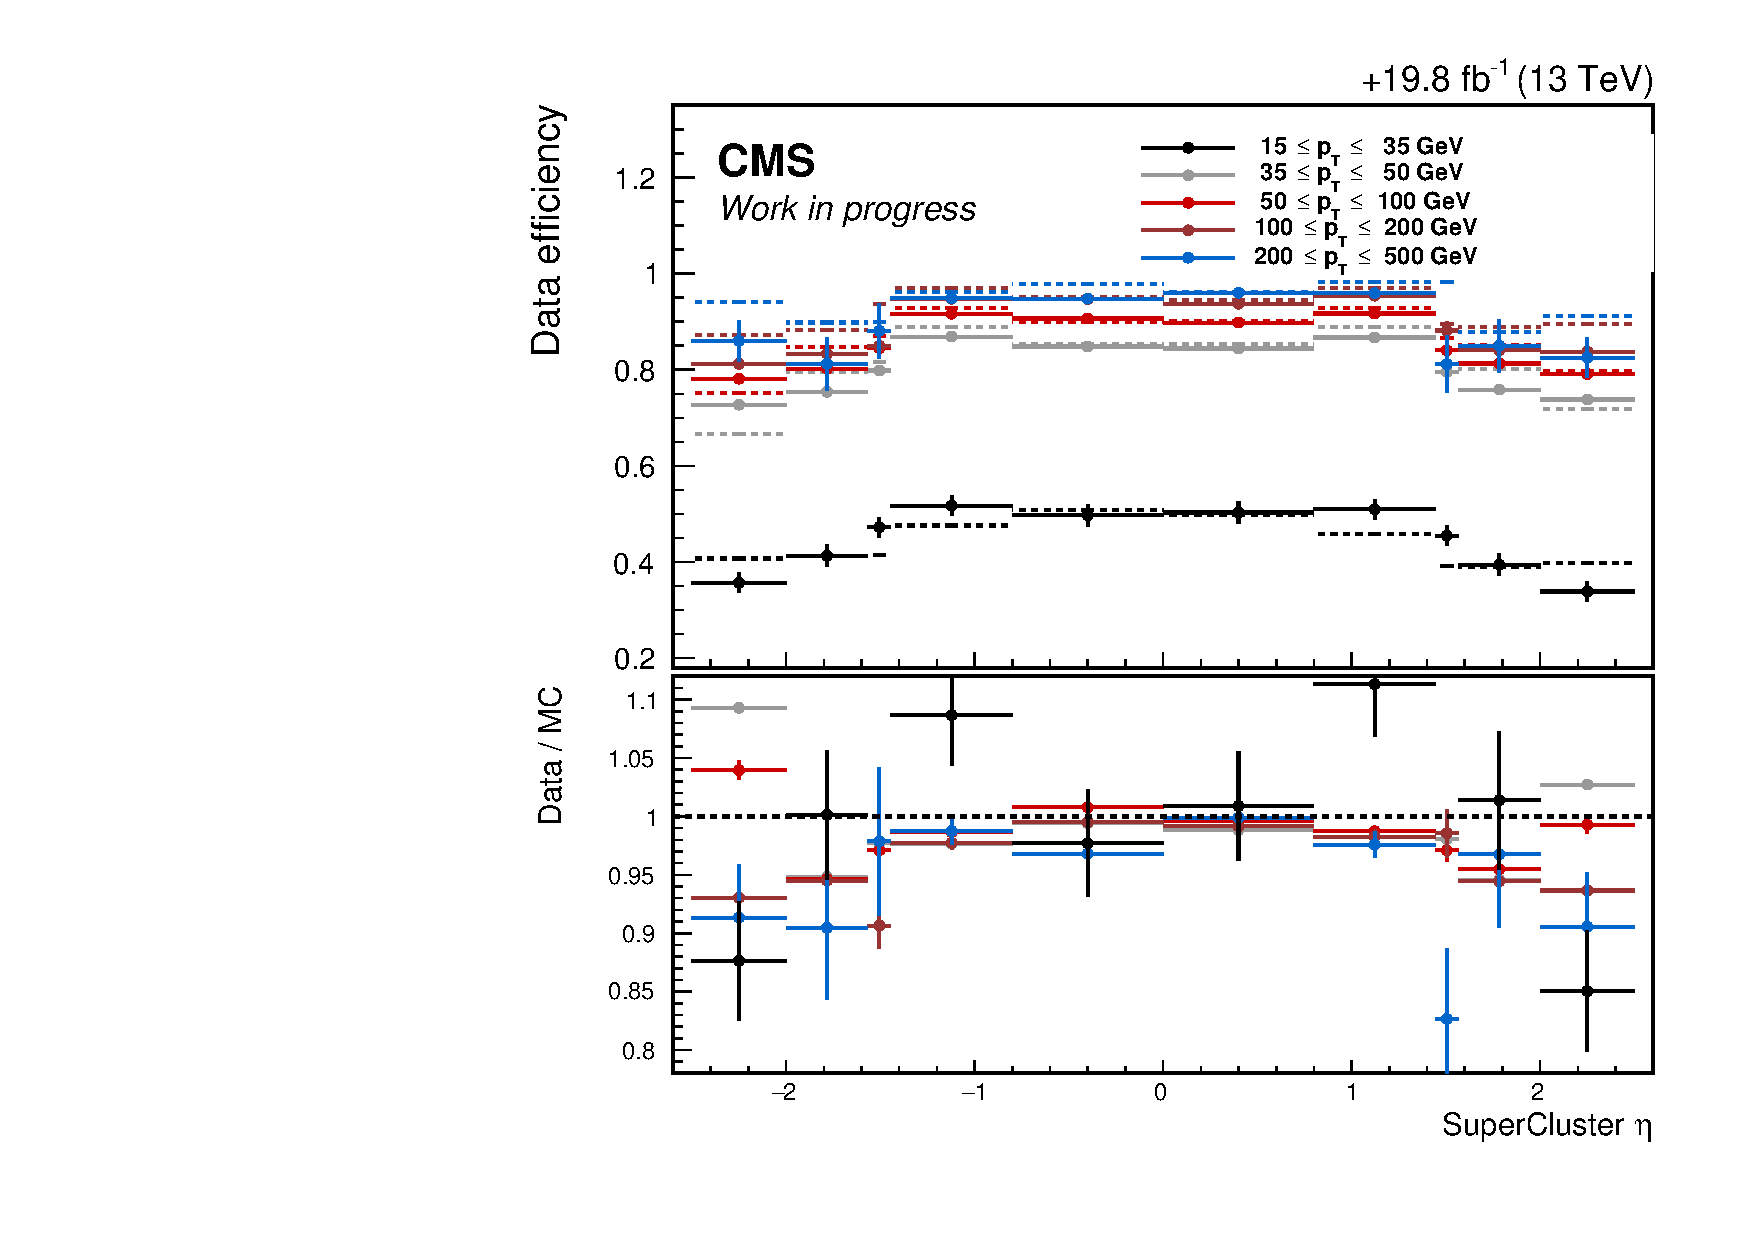
\includegraphics[width=\linewidth]{figs/05_analysis/UL2016_preVFP_SFvseta_myWP.pdf}
		\caption{2016 pre-VFP}
	\end{subfigure}
	\caption[Trigger efficiency as a function of $\eta_{sc}$ for several ranges of electron $\pt$ for all data taking eras.]{Trigger efficiency as a function of $\eta_{sc}$ for several ranges of electron $\pt$ for all data taking eras.}
	\label{fig:effVsEta_electronHLT}
\end{figure}

\begin{figure}[htb!]
	\centering
	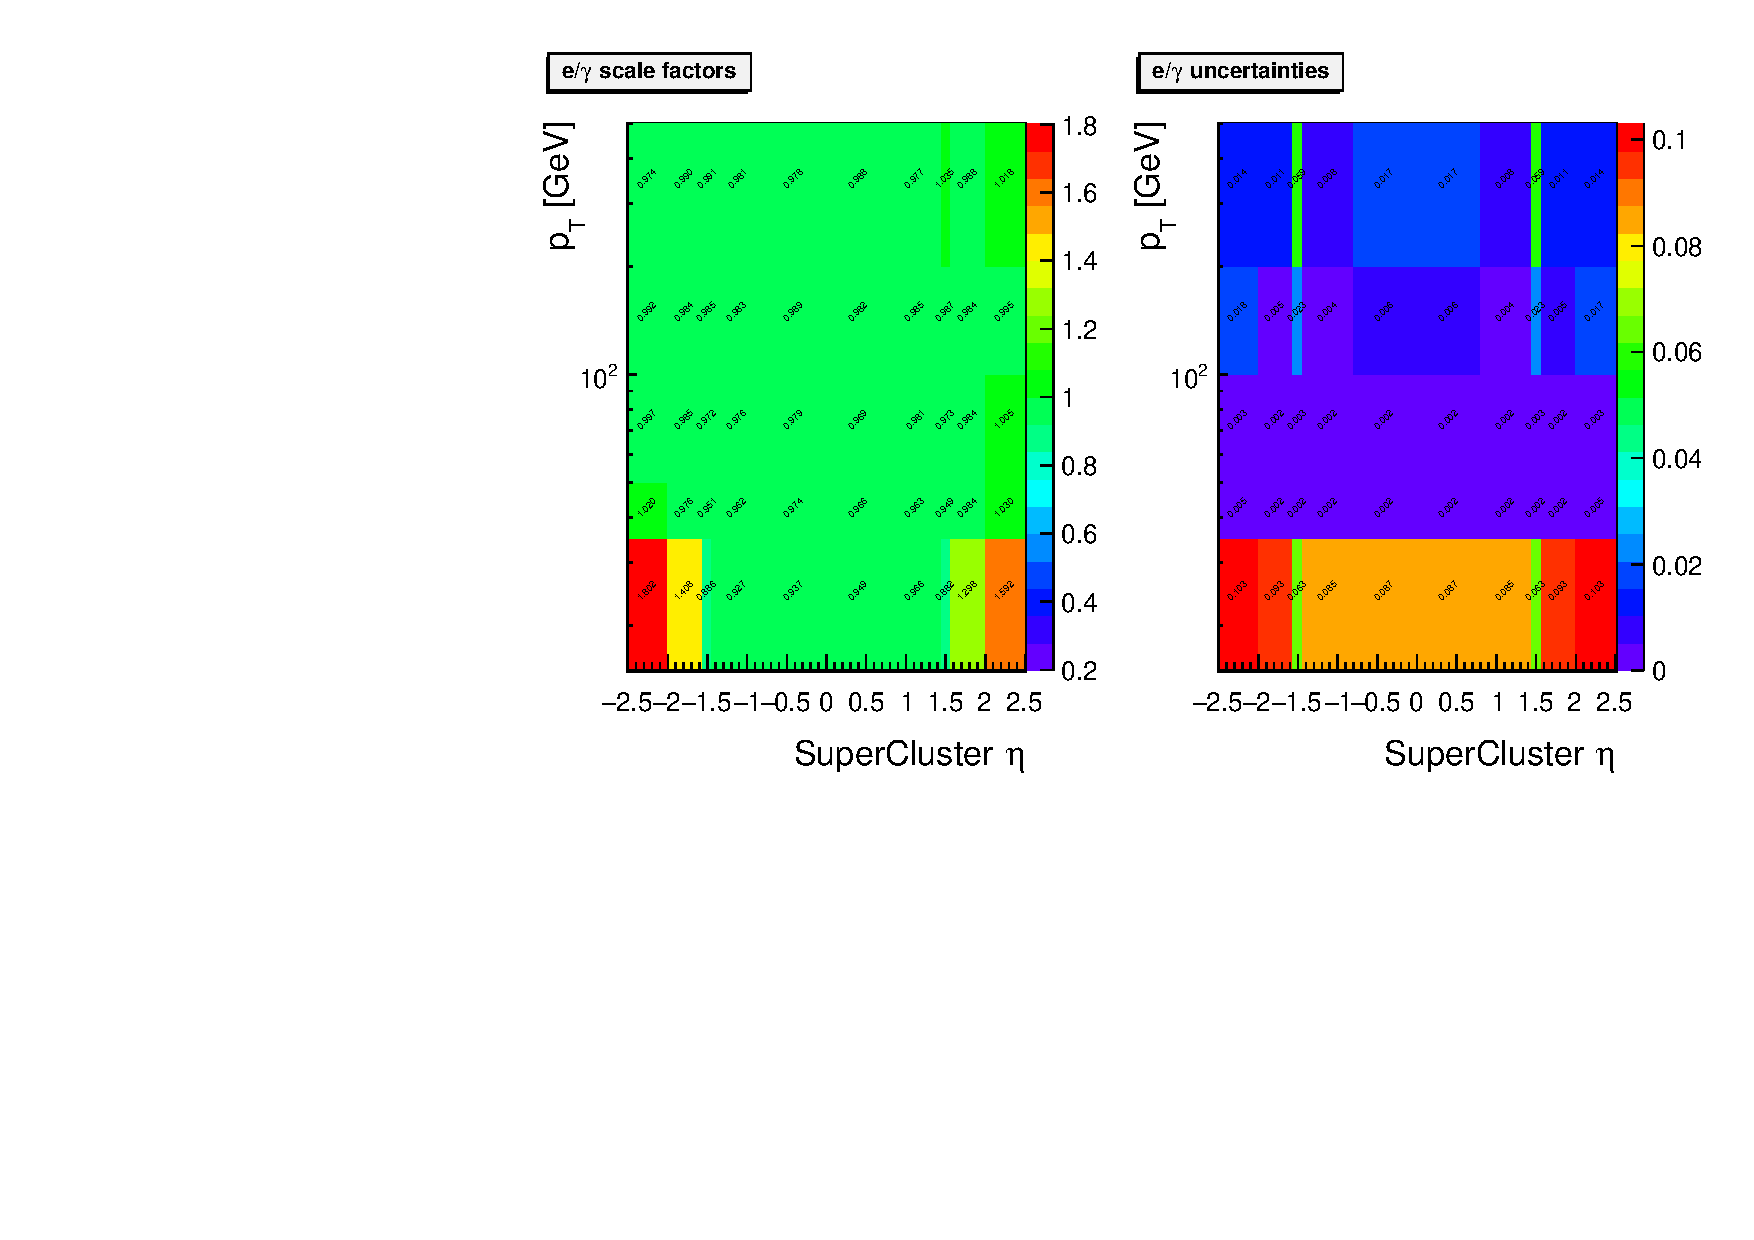
\includegraphics[width=0.85\linewidth]{figs/05_analysis/UL2018_SF2D_myWP.pdf}
	\caption[2018 electron HLT scale factors and uncertainties.]{2018 electron HLT scale factors and uncertainties.}
	\label{fig:UL2018_SF2D}
\end{figure}

\begin{figure}[htb!]
	\centering
	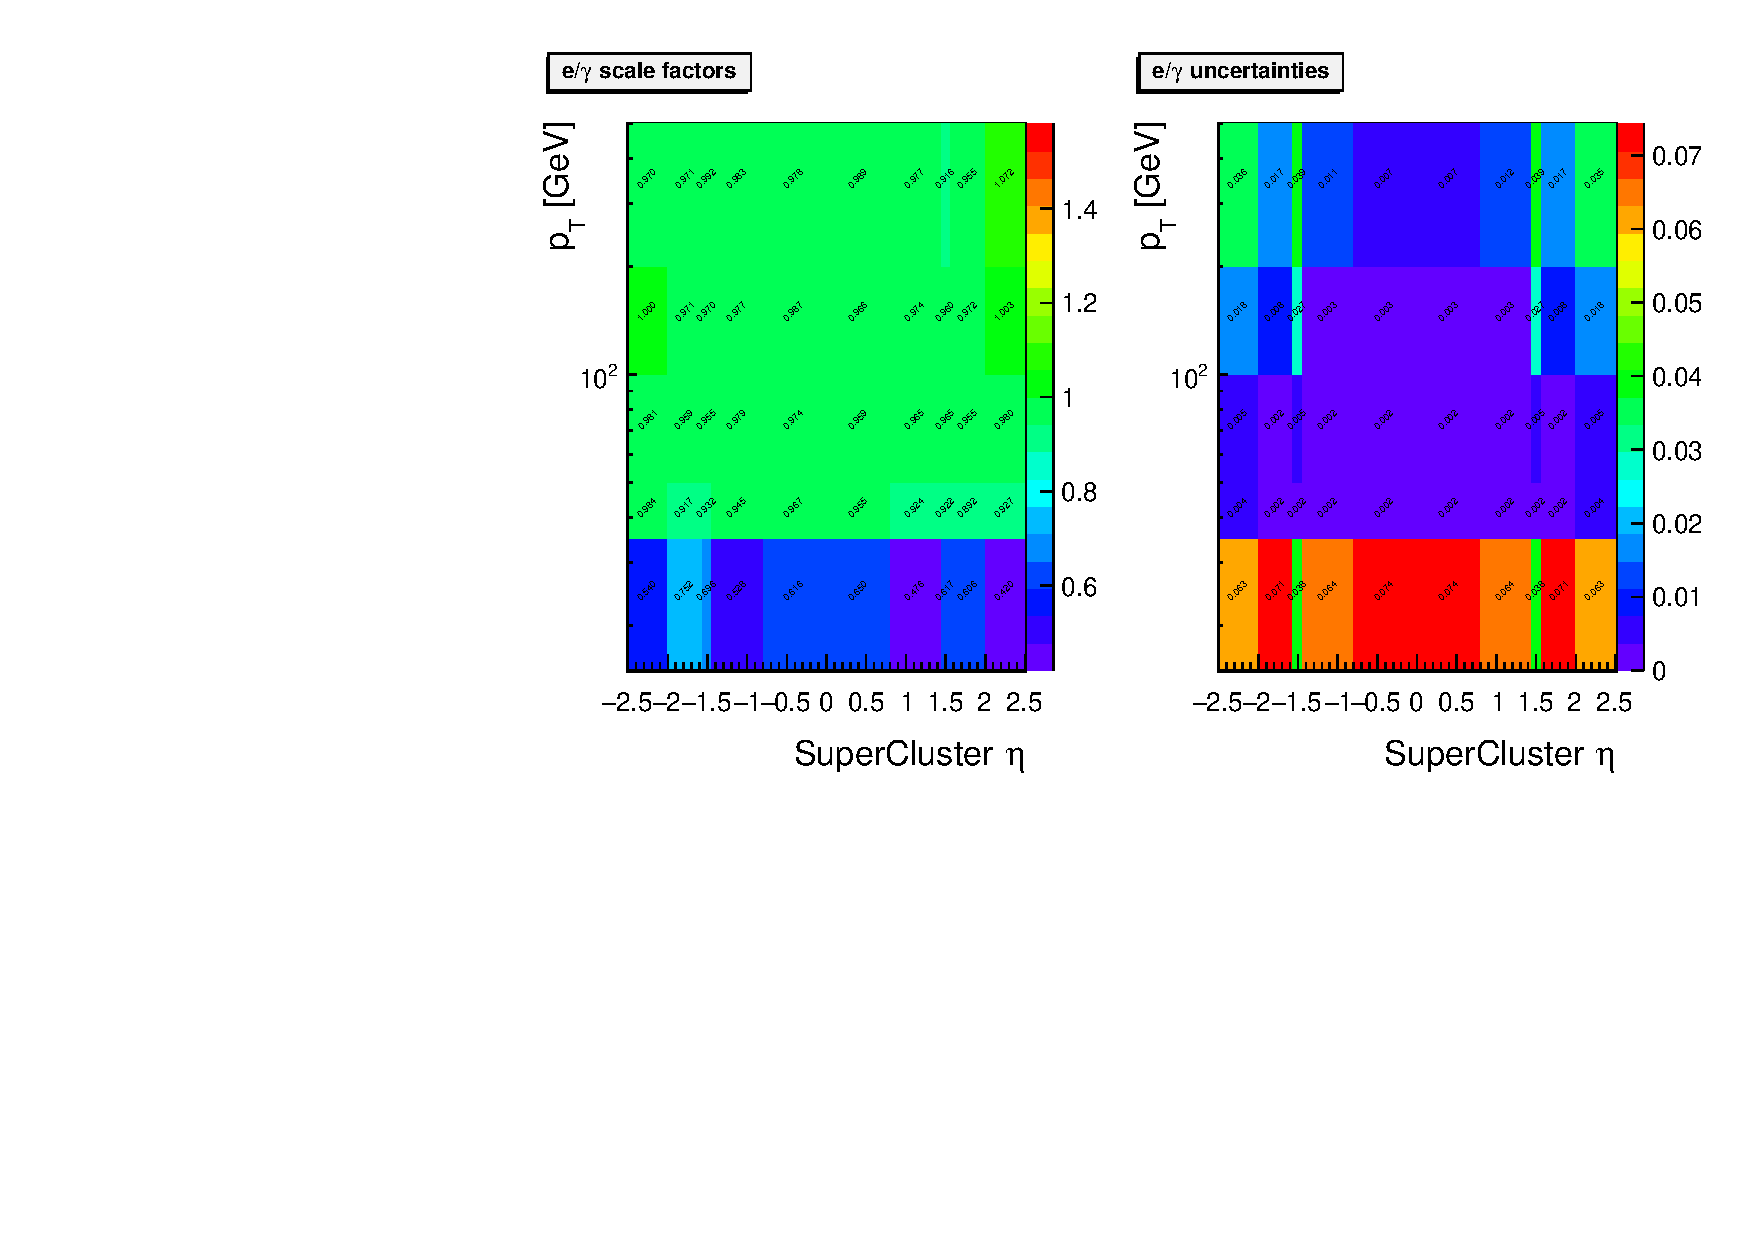
\includegraphics[width=0.85\linewidth]{figs/05_analysis/UL2017_SF2D_myWP.pdf}
	\caption[2017 electron HLT scale factors and uncertainties.]{2017 electron HLT scale factors and uncertainties.}
	\label{fig:UL2017_SF2D}
\end{figure}

\begin{figure}[htb!]
	\centering
	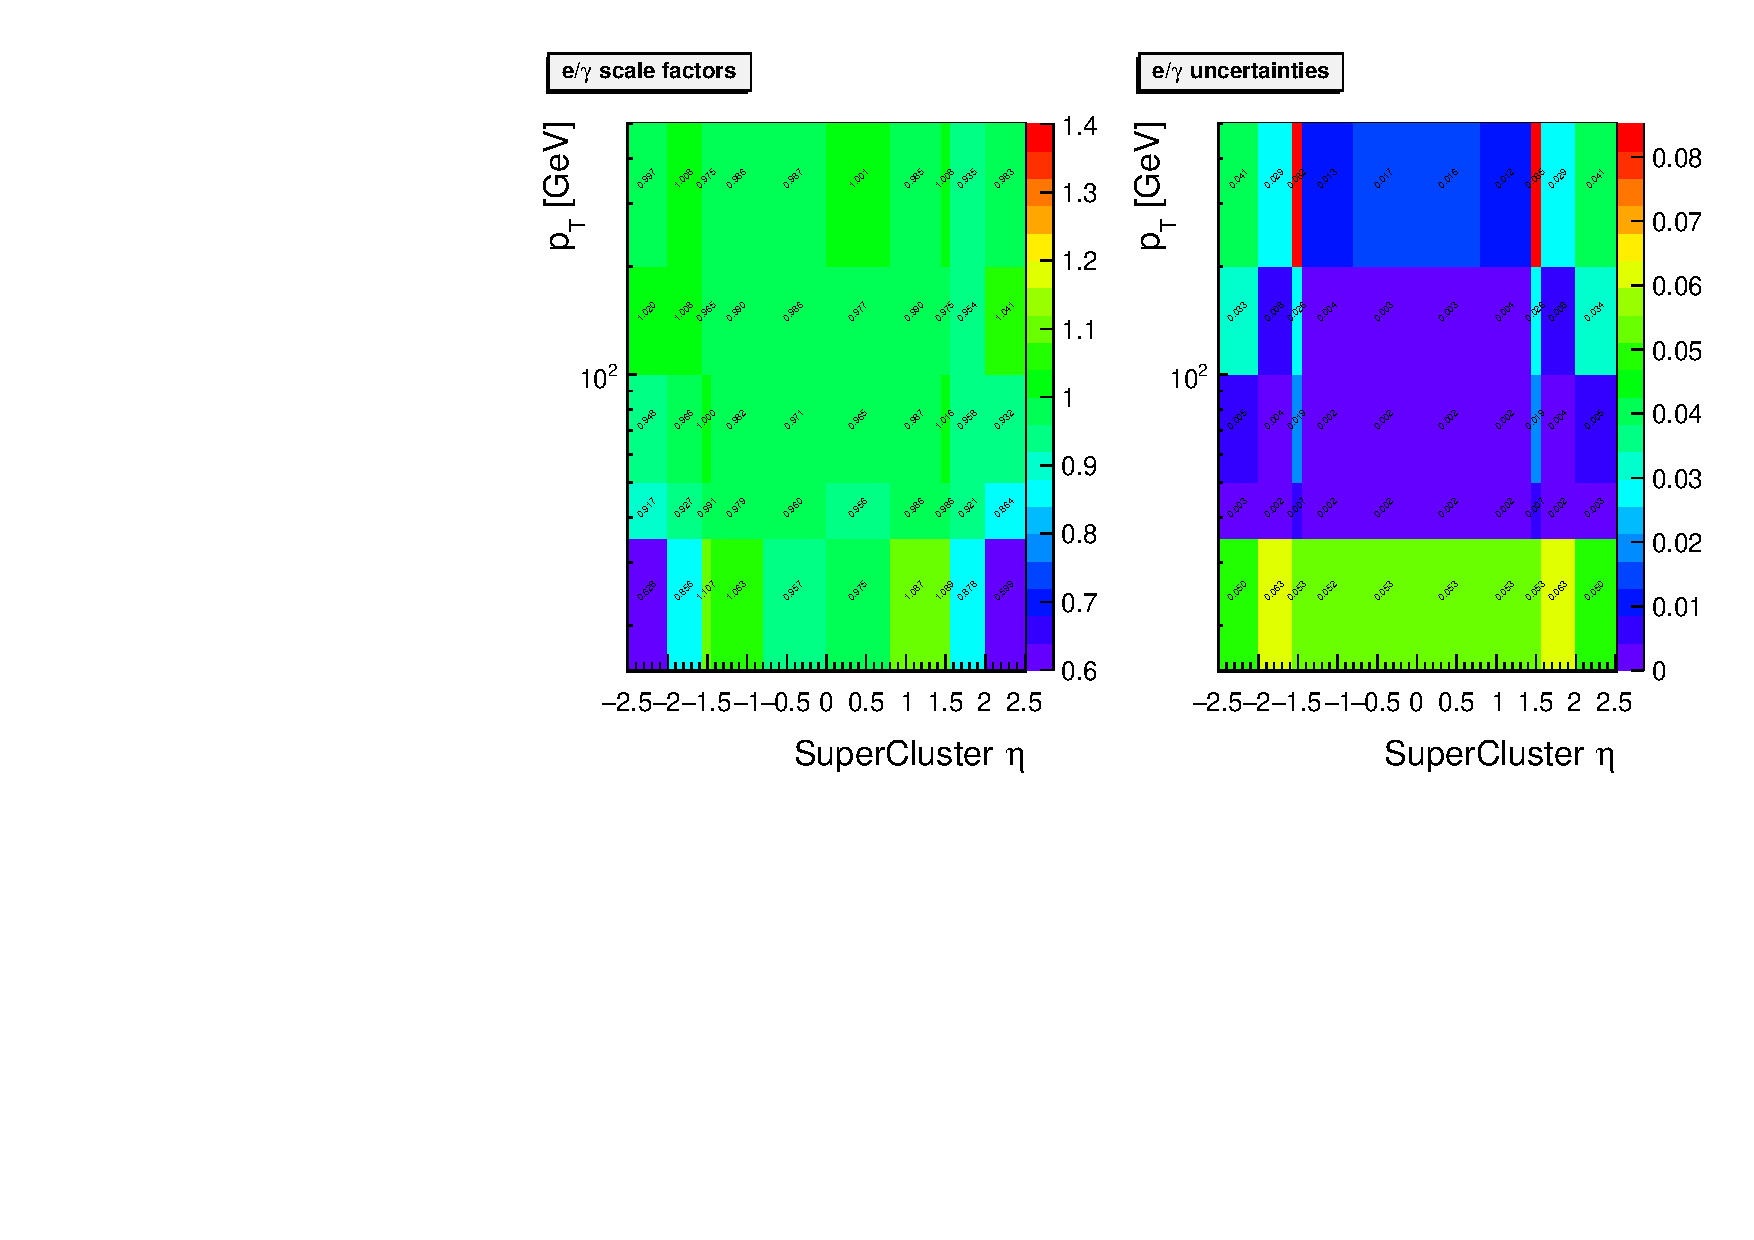
\includegraphics[width=0.85\linewidth]{figs/05_analysis/UL2016_postVFP_SF2D_myWP.pdf}
	\caption[2016 post-VFP electron HLT scale factors and uncertainties.]{2016 post-VFP electron HLT scale factors and uncertainties.}
	\label{fig:UL2016_postVFP_SF2D}
\end{figure}

\begin{figure}[htb!]
	\centering
	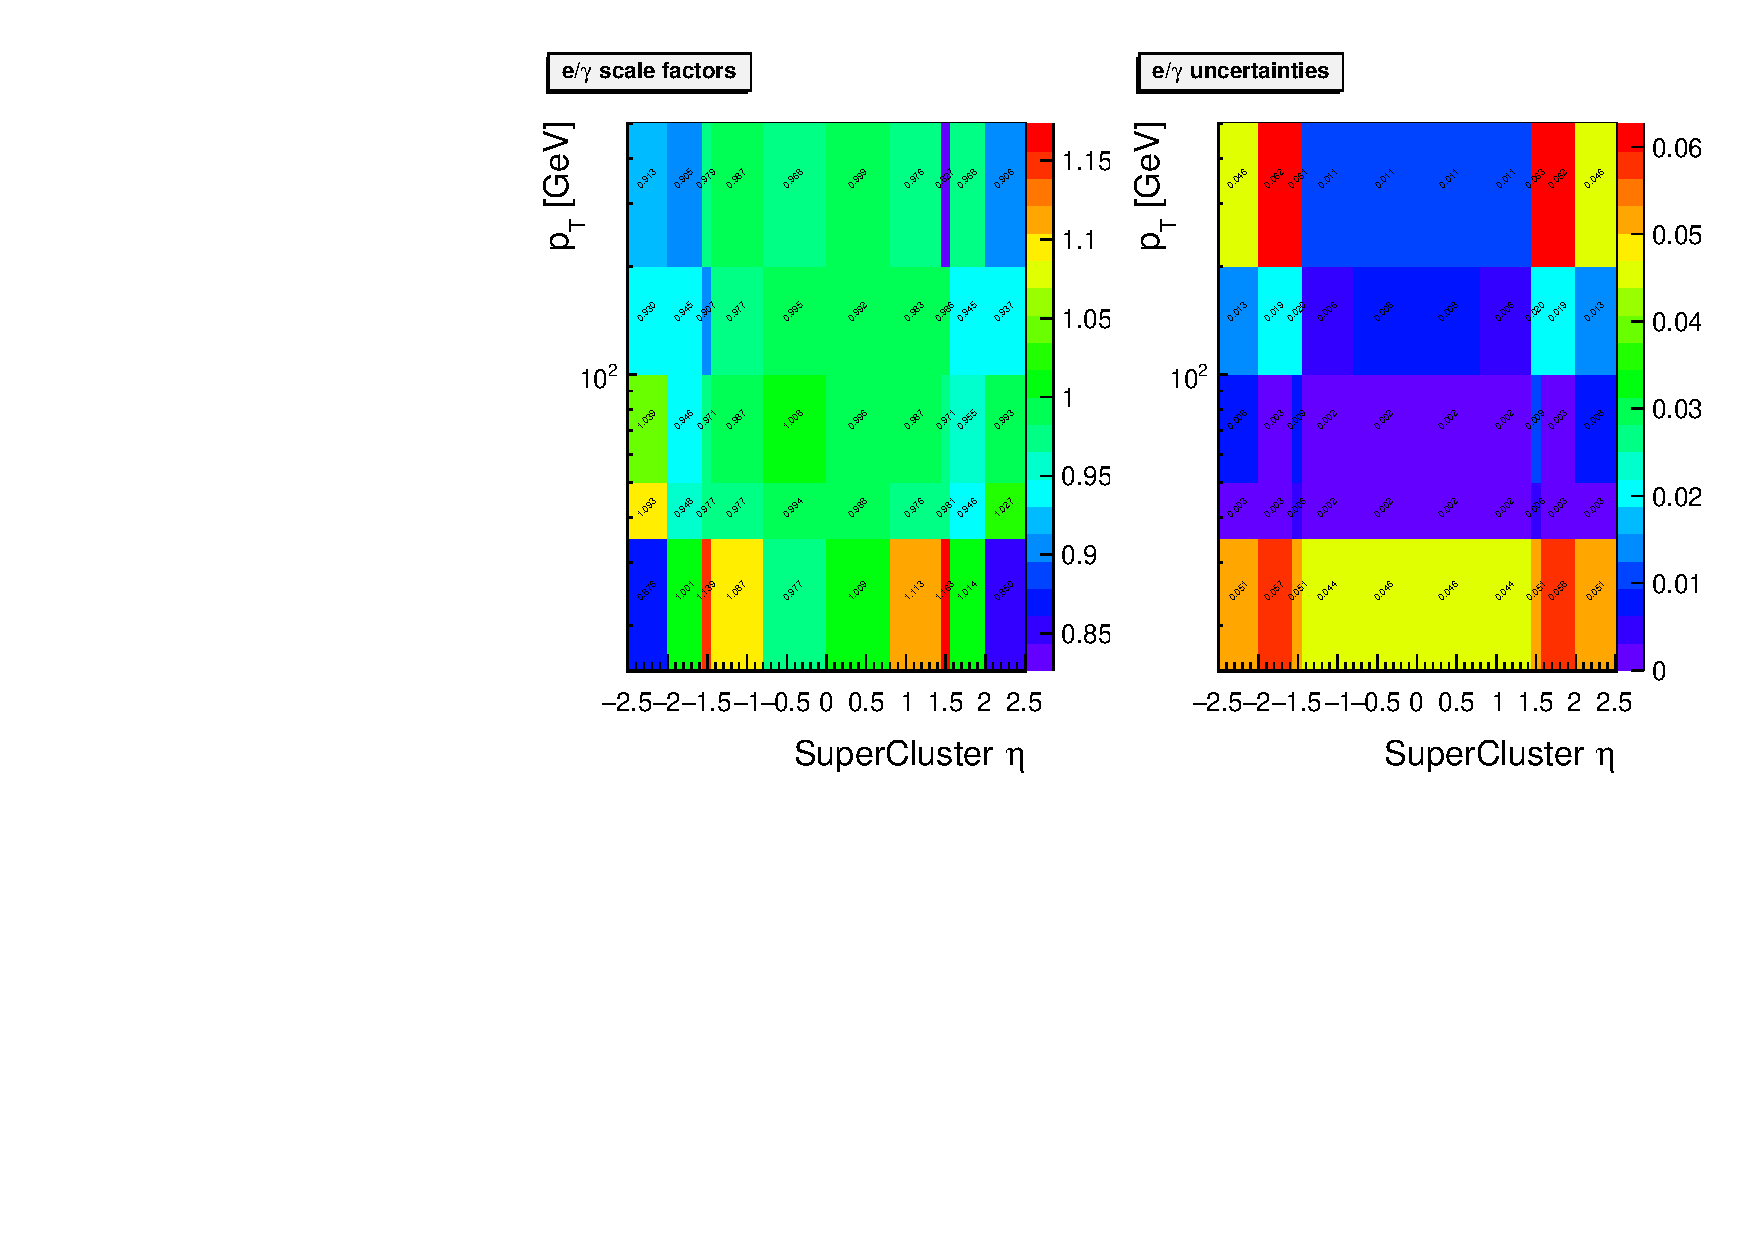
\includegraphics[width=0.85\linewidth]{figs/05_analysis/UL2016_preVFP_SF2D_myWP.pdf}
	\caption[2016 pre-VFP electron HLT scale factors and uncertainties.]{2016 pre-VFP electron HLT scale factors and uncertainties.}
	\label{fig:UL2016_preVFP_SF2D}
\end{figure}

Muon reconstruction, isolation, and ID scale factors are applied for each muon used to reconstruct the \PZ as a function of $\pt$ and $|\eta|$. Muon trigger scale factors are as a function of $\pt$, $\eta$ and charge of the triggering muon, or the higher \pt muon if both pass the single muon trigger. The photon ID and all electron scale factors are applied as a function of electron \pt and $\eta$, with the electron HLT scale factor application following the same logic as the muon HLT. Lastly, the photon pixel seed veto scale factor is applied as a function of the $\eta$ region (barrel or endcap) of the photons. Most scale factors are on the order of a few percent with uncertainties less than 0.1\%.


\section{Vertex Reconstruction of Displaced Photon Pairs} \label{sec:ana_vertex}
\subsection{Diphoton Kinematics} \label{sec:vertex_calc}
The kinematics of a long lived, massive scalar boson $\Phi$ decaying to two photons can be precisely described by the following
\begin{equation}\label{eq:me1e2theta}
	\text{m}_{\Phi}^2 = 2\text{E}_1\text{E}_2(1-\cos\theta)
\end{equation}
where the m$_\Phi$ is the mass of the $\Phi$, E$_1$ and E$_2$ are the energies of the two photons, and $\theta$ is the angle between the two photons. The energy of the two photons is measured by the CMS ECAL, thus $\theta$ can be calculated as a function of m$_\Phi$. Due to the primary vertex, decay vertex, and ECAL clusters being coplanar, this calculation is treated as a 2 dimensional problem. It is a trivial procedure to rotate the system to calculate the vertex, then rotate back to detector coordinates once the decay vertex is calculated. Let the position of the two ECAL clusters be \textbf{r$_1$} and \textbf{r$_2$}. The system can be rotated by an angle
\begin{equation} \label{eq:rot_angle}
	\varphi=\arccos\left(\frac{\textbf{r}_1\times\textbf{r}_2}{\|\textbf{r}_1\times\textbf{r}_2\|}\cdot\hat{z}\right)
\end{equation}
around an axis given by 
\begin{equation} \label{eq:rot_axis}
	\hat{n}=\frac{\textbf{r}_1\times\textbf{r}_2}{\|\textbf{r}_1\times\textbf{r}_2\|}\times\hat{z}
\end{equation}
to determine the decay vertex, then rotated by $-\varphi$ around the same axis to give the final value.

The geometry of the vertex fit is described in figure~\ref{fig:vertex_diagram}. Assume we have two ECAL clusters and a given value of m$_\Phi$. This fixes the value of $\theta$ from equation~\ref{eq:me1e2theta}. It will be shown that the locus of points satisfying these constraints corresponds to the arcs of two circles that overlap the ECAL clusters.

\begin{figure}[htb]
	\centering
	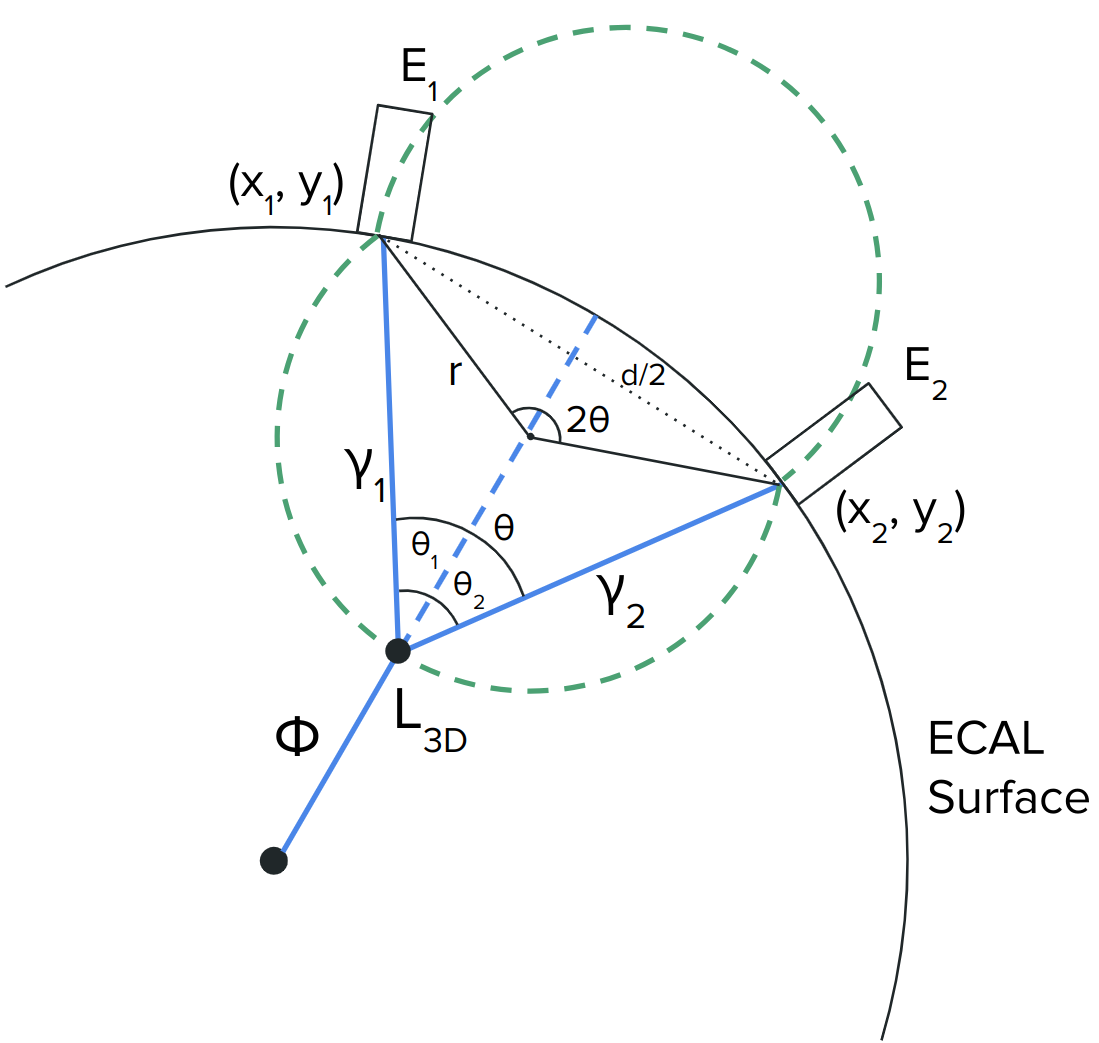
\includegraphics[width=0.65\linewidth]{figs/05_analysis/vertexfit_diagram.png}
	\caption{Geometrical configuration used to reconstruct the displaced vertex of the di-photon pair}
	\label{fig:vertex_diagram}
\end{figure}

Because three non-colinear points uniquely define a circle, $\theta$ corresponds to an inscribed angle on a circle which overlaps the decay vertex and the two ECAL clusters located at $(x_1, y_1)$ and $(x_2, y_2)$. The central angle of the arc between the two clusters has measure $2\theta$ by the inscribed angle theorem. From this, the radius of the circle can be defined by
\begin{equation} \label{eq:vertex_r}
	r=\frac{d}{2\sin{\theta}}
\end{equation}
where $d=\sqrt{(x_2-x_1)^2+(y_2-y_1)^2}$ is the distance between the two ECAL clusters. The center of the circle $(x_0, y_0)$ is constrained by the two ECAL cluster coordinates and the equation of a circle $(x-x_0)^2+(y-y_0)^2=r^2$, which can be solved to give
\begin{equation} \label{eq:vertex_x0}
	x_0=\frac{x_1+x_2}{2}\pm\frac{y_1-y_2}{\text{q}}\cdot\sqrt{\text{r}^2-\frac{\text{q}^2}{4}}
\end{equation}
\begin{equation} \label{eq:vertex_y0}
	y_0=\frac{y_1+y_2}{2}\pm\frac{x_2-x_1}{\text{q}}\cdot\sqrt{\text{r}^2-\frac{\text{q}^2}{4}}
\end{equation}
\begin{equation} \label{eq:vertex_q}
	\text{where q}=\sqrt{(x_1-x_2)^2+(y_1-y_2)^2}
\end{equation}
The two solutions represent circles centered inside and outside of the ECAL. If $\theta<\pi/2$, then only the major arcs of the two circle satisfy equation~\ref{eq:me1e2theta}. Alternatively, if $\theta>\pi/2$ only the minor arcs are valid solutions. For either solution, an arc from one of two  circles will lie outside the ECAL. This arc represents a nonphysical solution and can be discarded, as it would imply the $\Phi$ both decayed outside of the ECAL and left ECAL clusters. The remaining arc represents the locus of possible decay vertices.

The angle between the two photons can be divided into the deflection of each photon ($\theta_1$ and $\theta_2$ respectively), and conservation of momentum requires $E_1\sin{\theta_1}-E_2\sin{\theta_2}=0$. From here, the vertex can be calculated numerically by sampling points along the remaining arc and choosing the coordinates that satisfy this equation.

It should be noted that this method can yield a locus of points that pass behind the beamline resulting in a negative impact parameter. The vertex is still calculated in these cases in order to provide a disjoint region with respect to the signal region that will be used to validate analysis methods and estimate the background yield. A diagram showing a negative reconstructed vertex is shown in figure~\ref{fig:negLxy}.

\begin{figure}[htb]
	\centering
	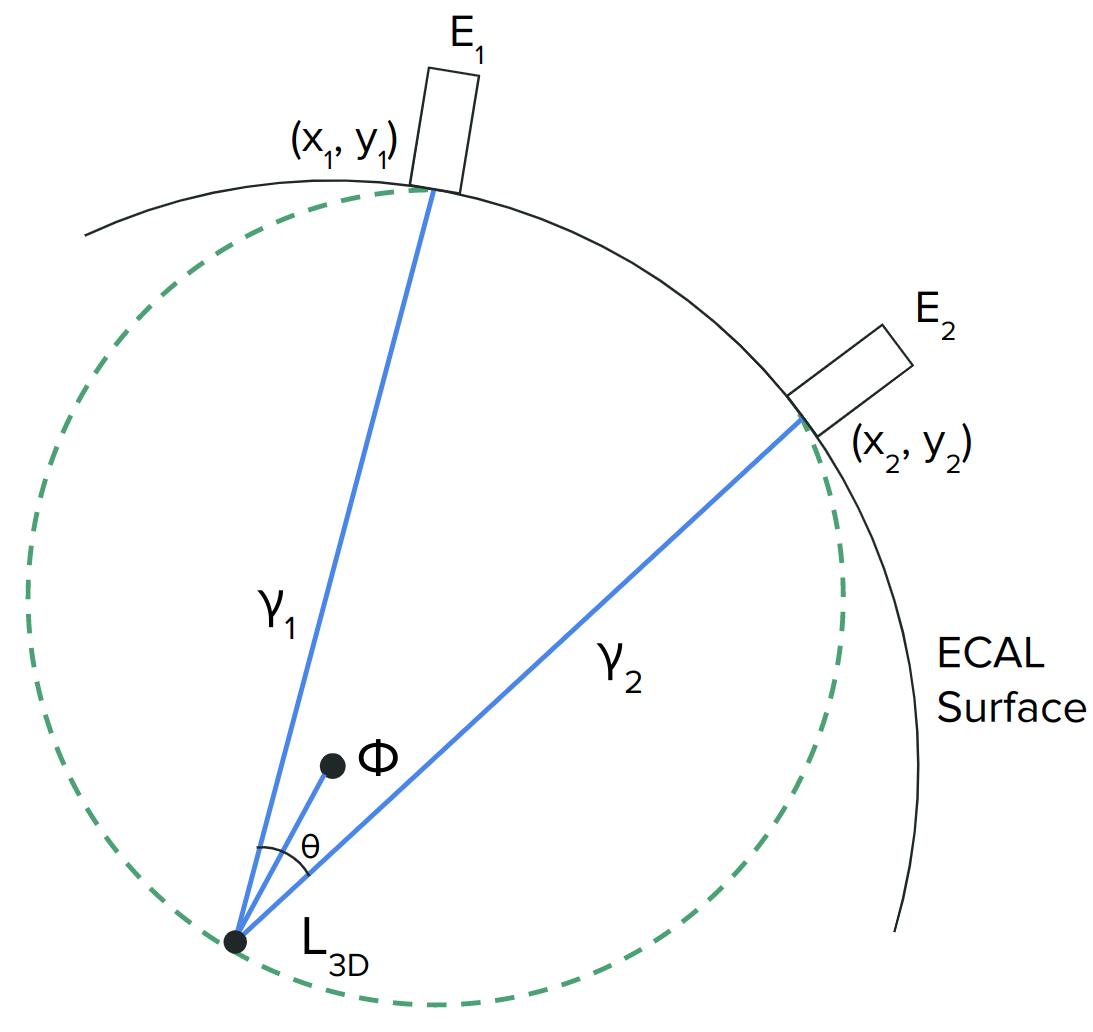
\includegraphics[width=0.65\linewidth]{figs/05_analysis/vertexfit_diagram_negativeLxy.png}
	\caption{Geometrical configuration showing the reconstruction of a negative impact parameter}
	\label{fig:negLxy}
\end{figure}

\subsection{Performance of the Diphoton Vertex Calculation}\label{sec:ana_vertex_results}
It is evident that since the kinematic fit uses the hypothetical mass of the $\Phi$, the fit must be rerun for every hypothetical mass used in this analysis. As a result, the events in the signal region used for each value of $m_\Phi$ are different. Figure~\ref{fig:lxys_a} shows the reconstructed \lxy behaves as expected as the $\Phi$ lifetime increases. To demonstrate the resolution of the kinematic fit, we plot the difference between the calculated \lxy and the generator level \lxy as a function of the generator level \lxy, performed using a $\PZ\to\ell\ell$ samples with m$_\Phi=30\GeV$, using both the c$\tau=100\unit{mm}$ and $1000\unit{mm}$ samples. These distributions can be seen in figure~\ref{fig:lxys_b}. The vertical slices of this histogram were fit to Gaussian distributions so that the mean and sigma could be plotted as a function of generator level \lxy. The means shown in figure~\ref{fig:lxys_c} show the differences in calculated and generator \lxy are compatible with zero, and the sigma shown in figure~\ref{fig:lxys_d} show a resolution of $<3\unit{cm}$, slightly decreasing with generator level $\lxy$. Both the mean and sigma remain consistent across all ranges of m$_\Phi$. The mean has a slight bias towards underestimating the \lxy due to the non-linear relation between the ECAL position/energy resolution and the vertex calculation. The sigma tends to decrease slightly as \lxy increases, as the $\Phi$ decaying closer to the ECAL means the photons traverse less material before reaching the ECAL. This gives a lower probability to interact with the tracker which improves the position and energy resolution.

\begin{figure}[htb!]
	\centering
	\captionsetup[subfigure]{justification=centering}
	\begin{subfigure}[h]{0.45\linewidth}
		\centering
		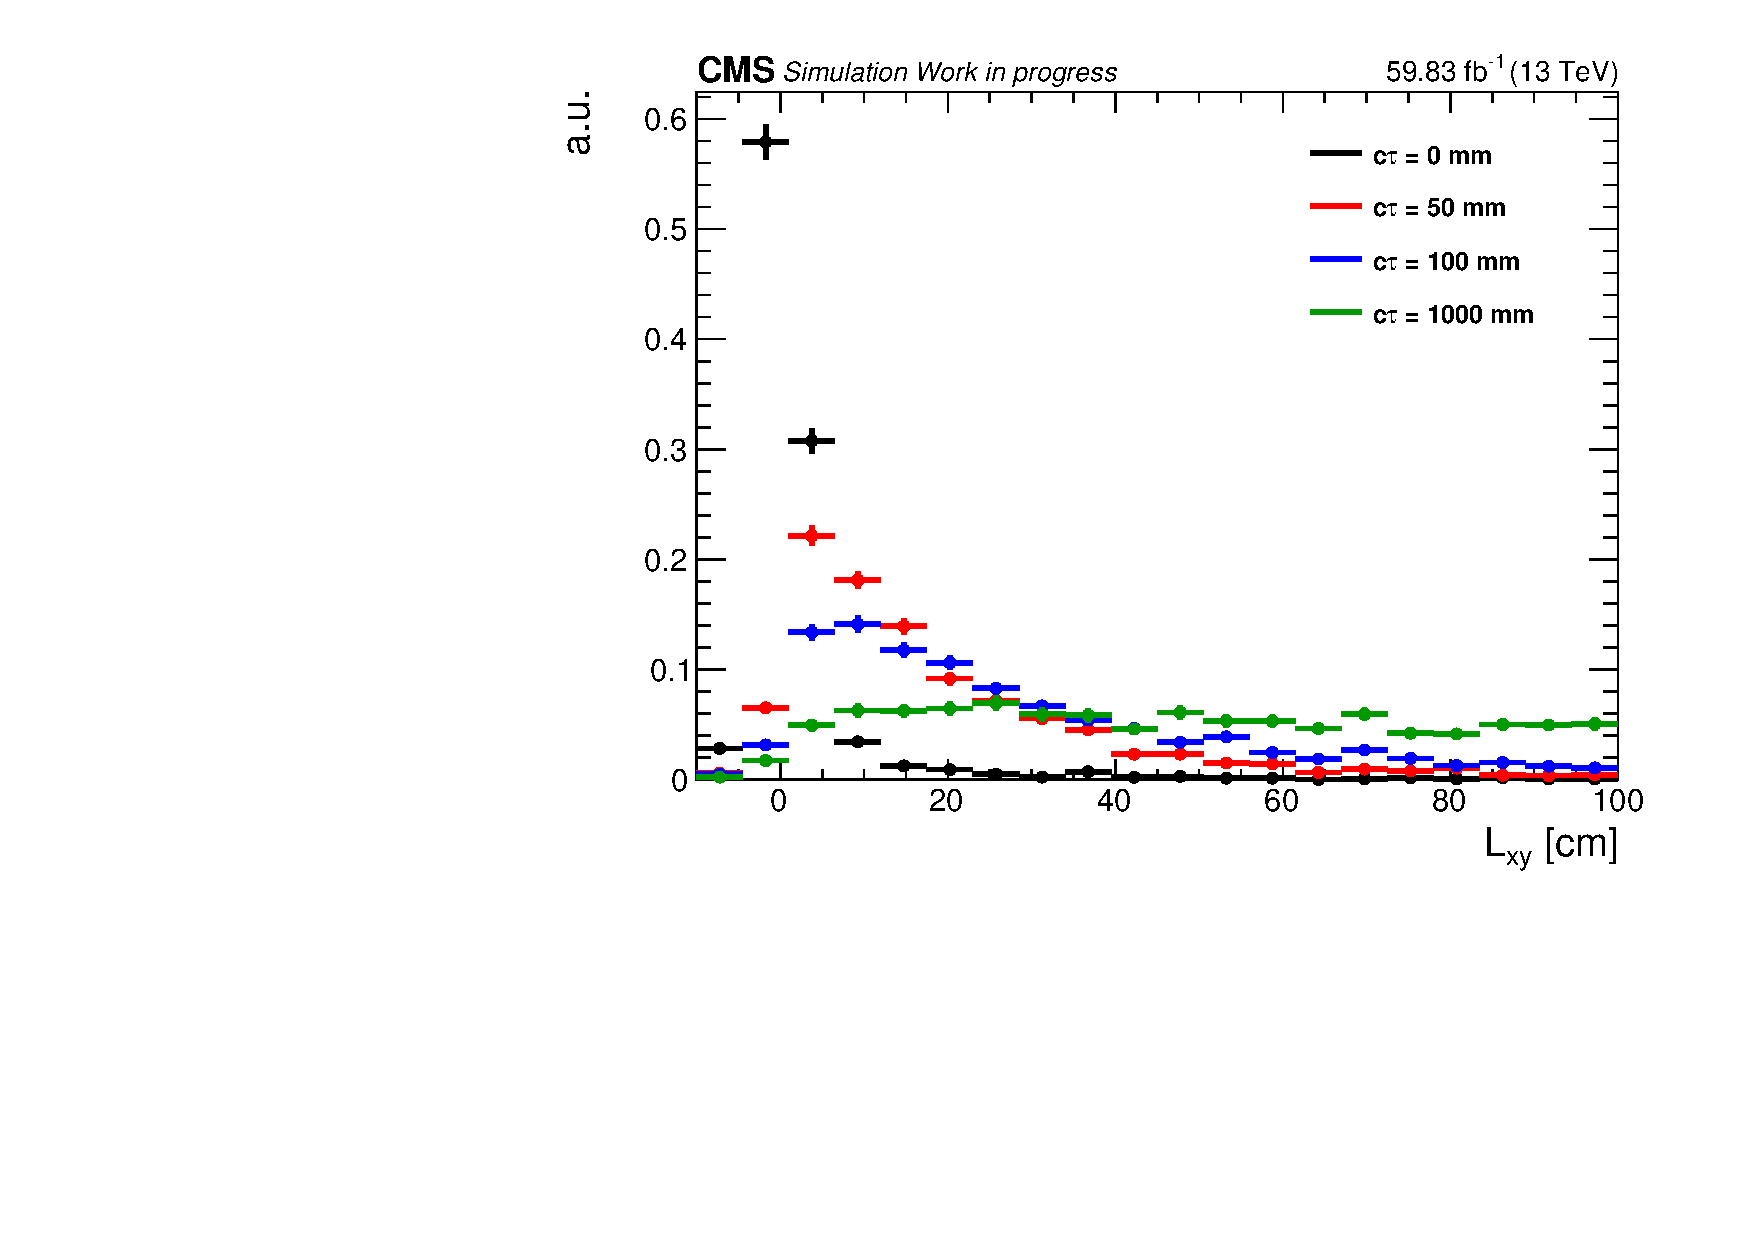
\includegraphics[width=\linewidth]{figs/05_analysis/2018_signalLxy_comparison.pdf}
		\caption{\lxy distribution calculated for $m_\Phi=30\GeV$, $\PZ\to\ell\ell$ signal samples}
		\label{fig:lxys_a}
	\end{subfigure}
	\begin{subfigure}[h]{0.45\linewidth}
		\centering
		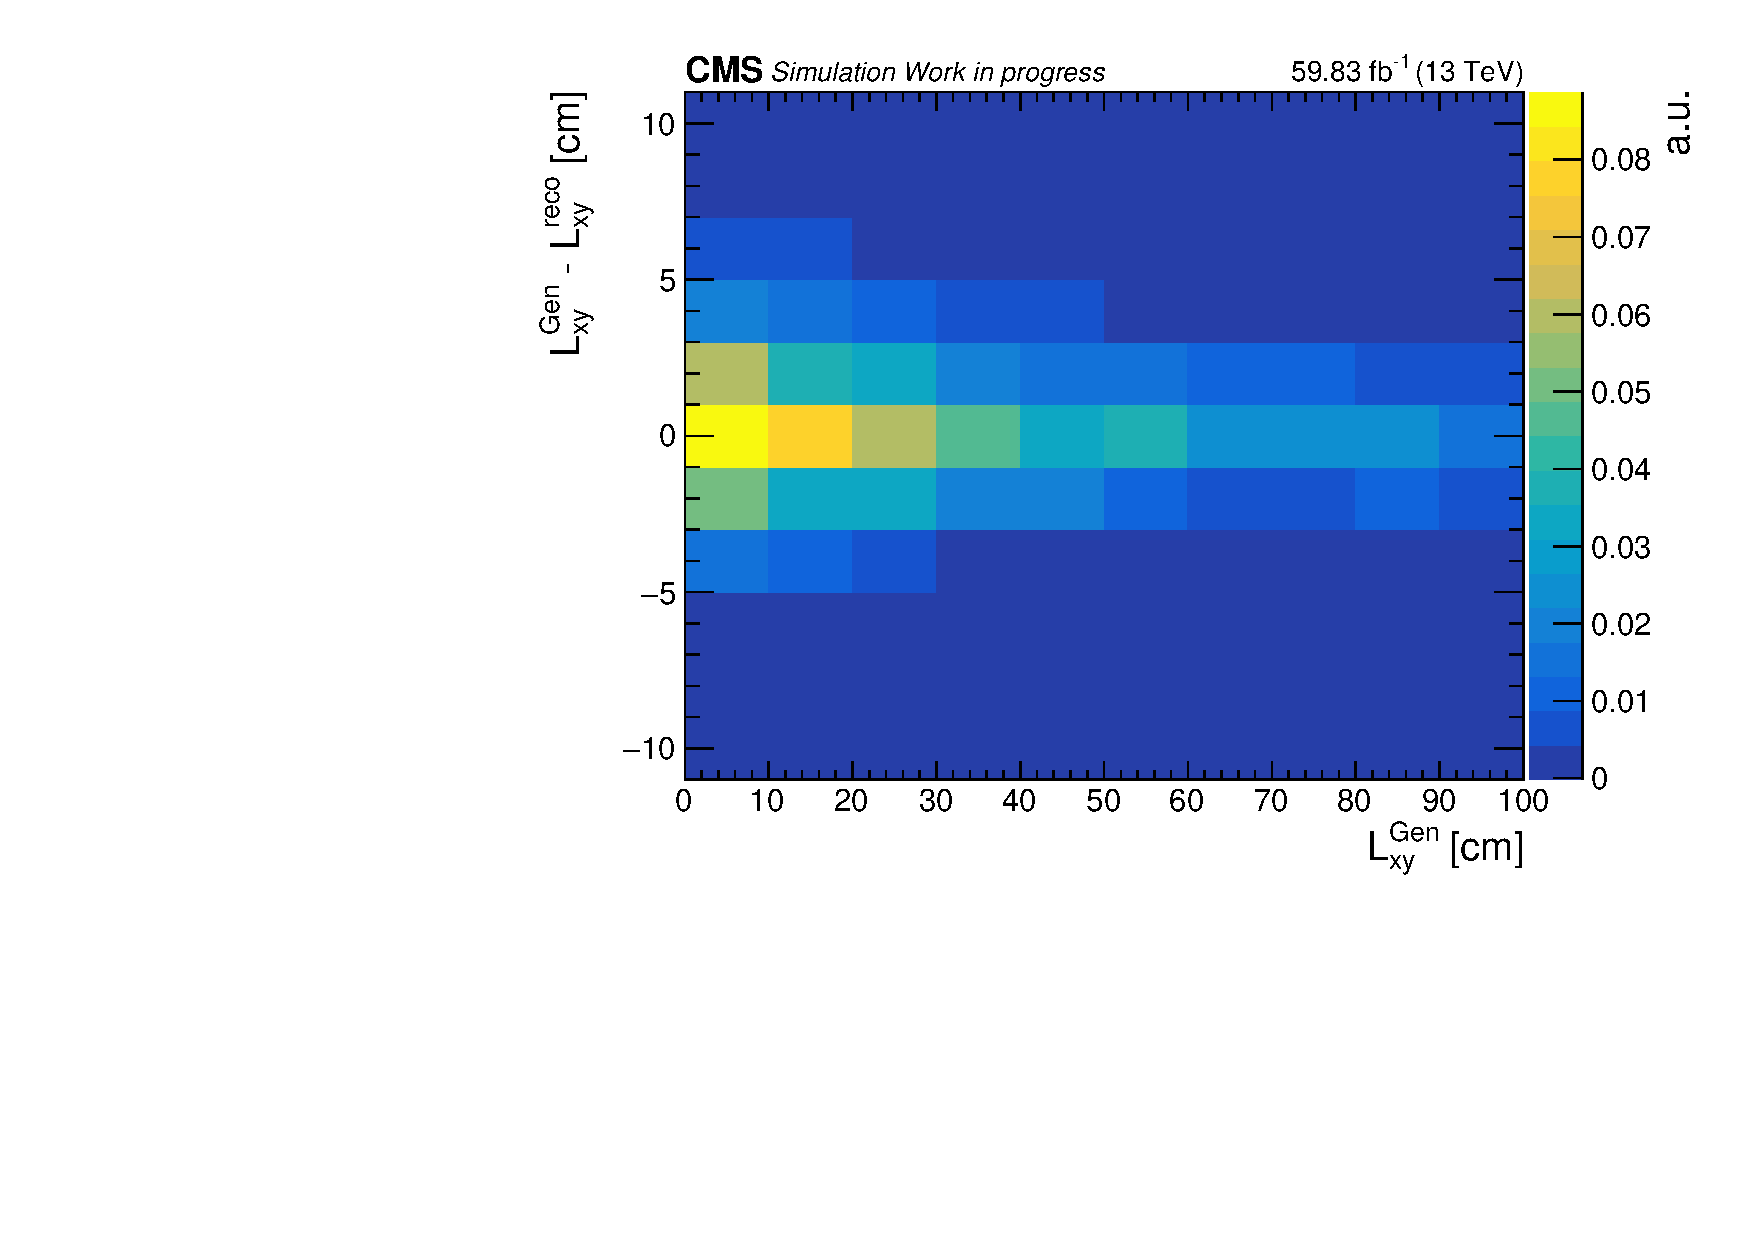
\includegraphics[width=\linewidth]{figs/05_analysis/2018_deltaLxyVsLxy_Z_m30.pdf}
		\caption{The $\Delta\lxy$ vs $\lxy$ distributions for signal events with exactly 2 photons}
		\label{fig:lxys_b}
	\end{subfigure}
	\begin{subfigure}[h]{0.45\linewidth}
		\centering
		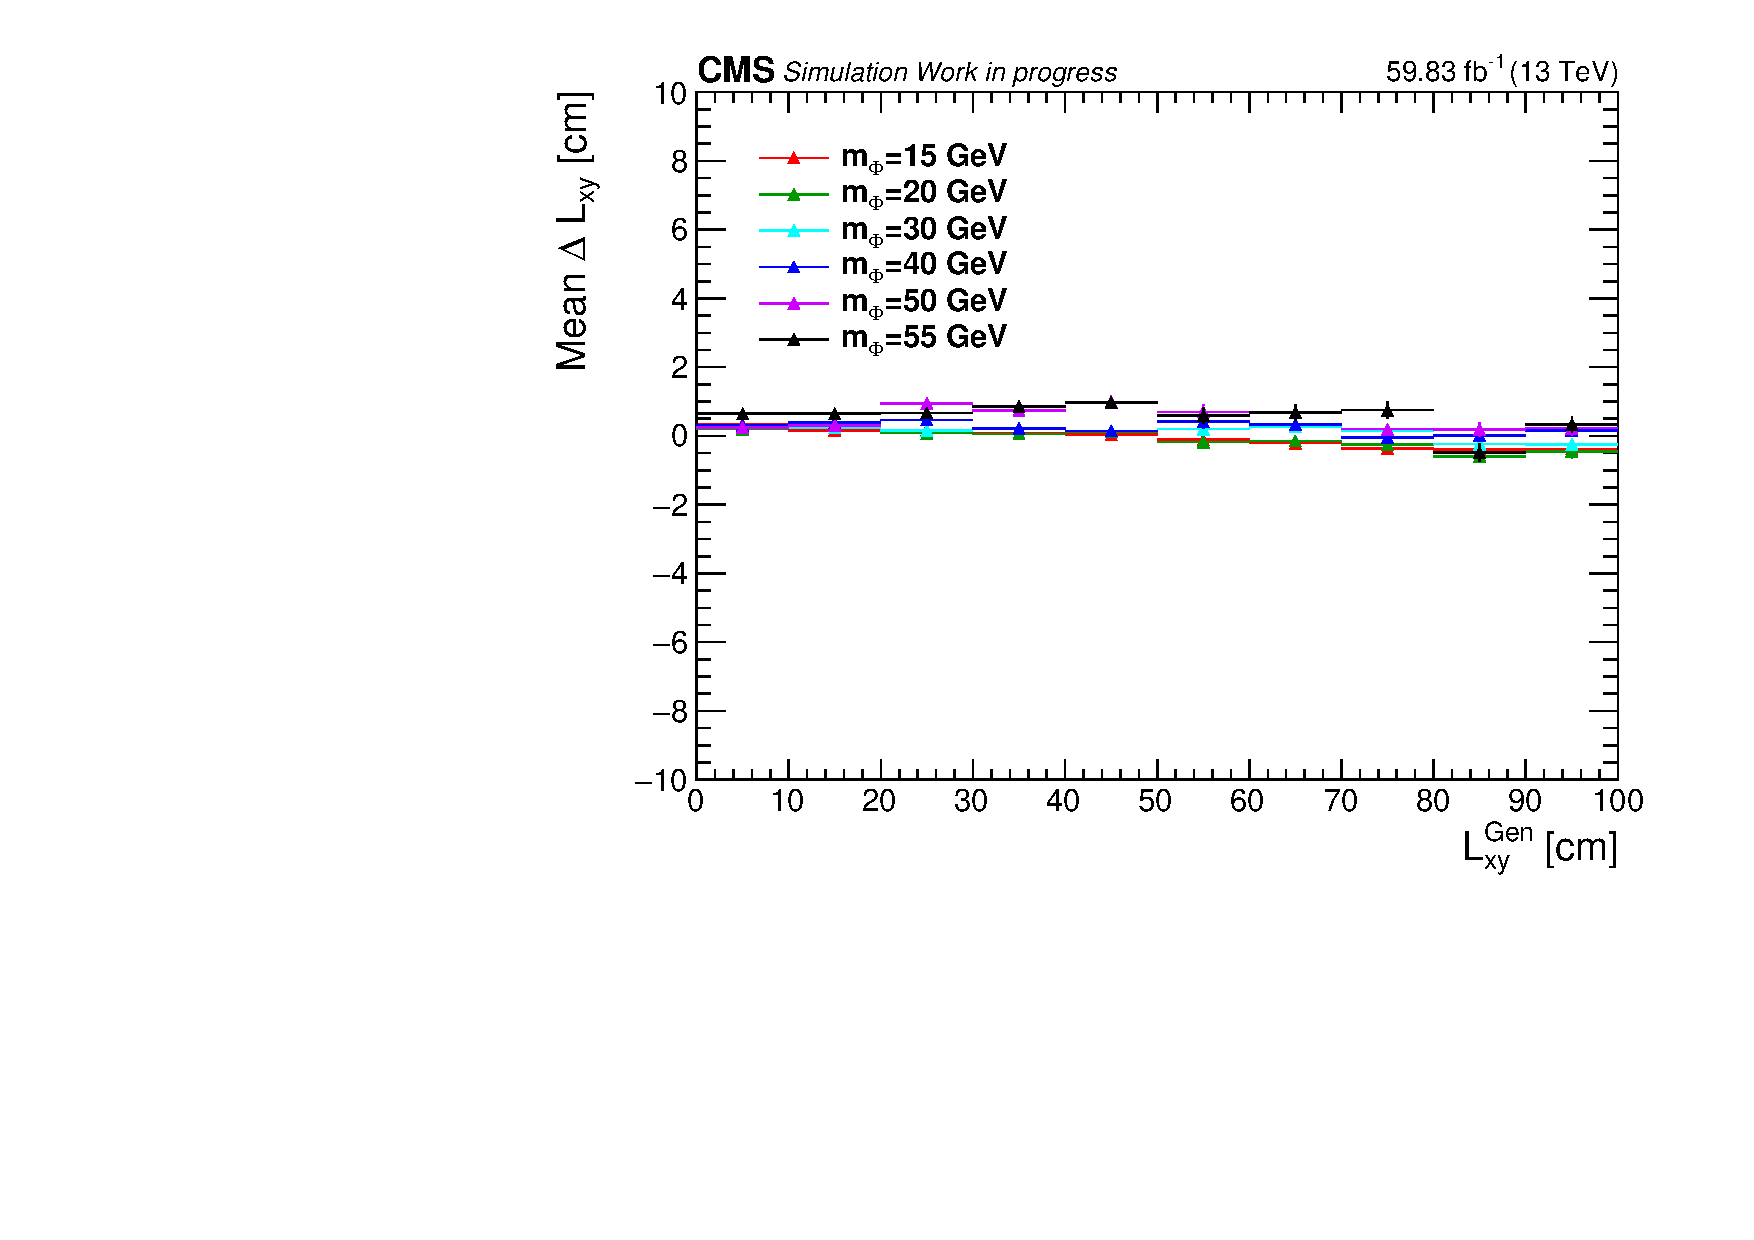
\includegraphics[width=\linewidth]{figs/05_analysis/2018_meanLxyVsLxy_Z_all.pdf}
		\caption{Mean of Gaussian slice fits}
		\label{fig:lxys_c}
	\end{subfigure}
	\begin{subfigure}[h]{0.45\linewidth}
		\centering
		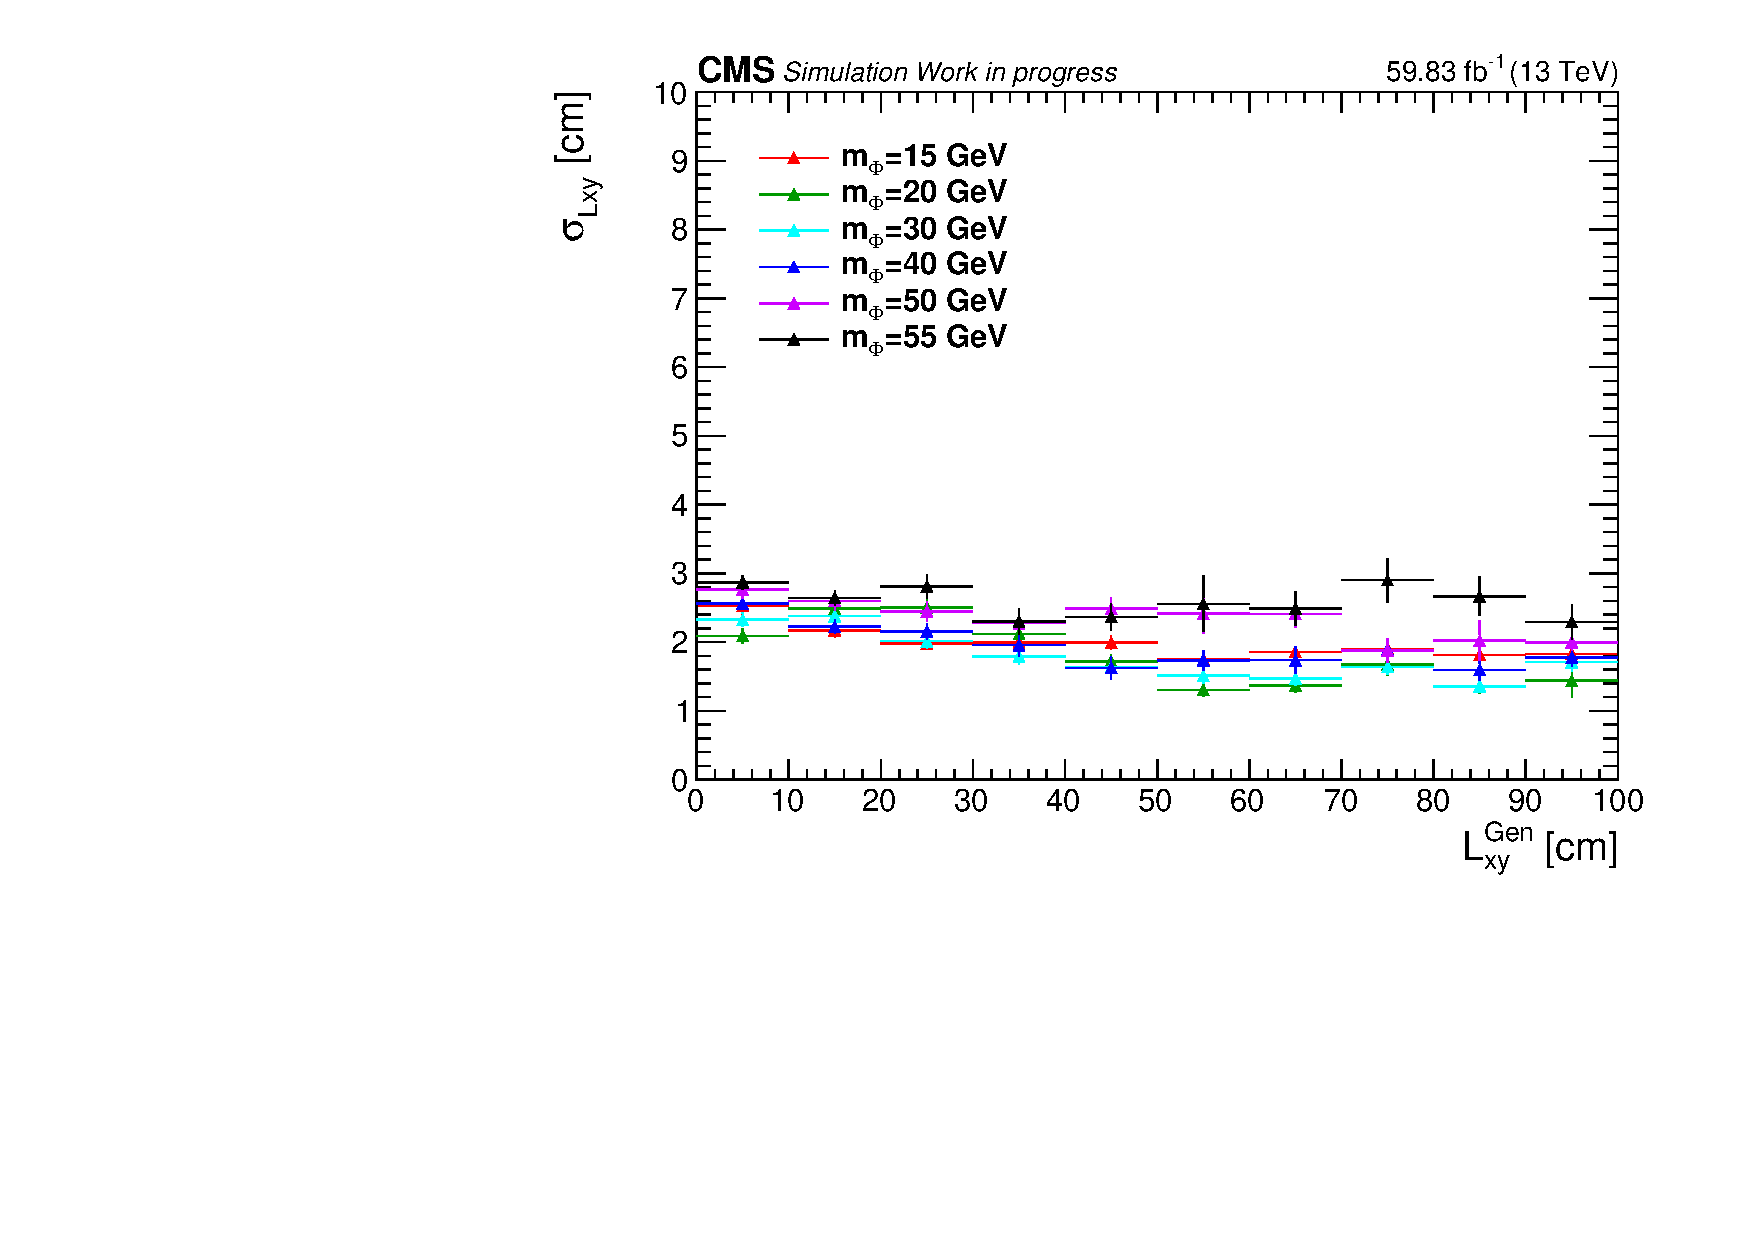
\includegraphics[width=\linewidth]{figs/05_analysis/2018_sigmaLxyVsLxy_Z_all.pdf}
		\caption{Sigma of Gaussian slice fits}
		\label{fig:lxys_d}
	\end{subfigure}
	\caption[Performance of the vertex calculation on signal samples. The fit shows good agreement across all values of generator level \lxy and a resolution of $<3\unit{cm}$.]{Performance of the vertex calculation on signal samples. The fit shows good agreement across all values of generator level \lxy and a resolution of $<3\unit{cm}$.}
	\label{fig:lxys}
\end{figure}

It can be shown that the calculated \lxy for a fixed value of prompt invariant photon mass \mgg is monotonically decreasing with the assumed value of \mphi. Assume that two photons have a prompt (four momenta calculated assuming the two clusters originated from the PV) invariant mass \mgg. Calculating the vertex assuming $\mphi=\mgg$ would yield a vertex with $\lxy=0$ by construction. Calculating the vertex assuming $\mphi>\mgg$ would cause the angle between the two photons given by equation~\ref{eq:me1e2theta} to decrease. As the ECAL cluster positions are fixed, this pushes the vertex backwards yielding $\lxy<0$. By similar methods, assuming a value of $\mphi<\mgg$ yields a vertex with $\lxy>0$. The dependence makes the \lxy very sensitive to small changes in the assumed value of \mphi. If the assumed value of \mphi differs from the true mass by $5\GeV$, the calculated \lxy can skew upwards or downwards by $>20\unit{cm}$, depending on the value of the true mass. Figure~\ref{fig:deltaLxy} shows the differences in generated and reconstructed \lxy, combining samples for all lifetimes for a given true mass.

\begin{figure}[htb!]
	\centering
	\captionsetup[subfigure]{justification=centering}
	\begin{subfigure}[h]{0.45\linewidth}
		\centering
		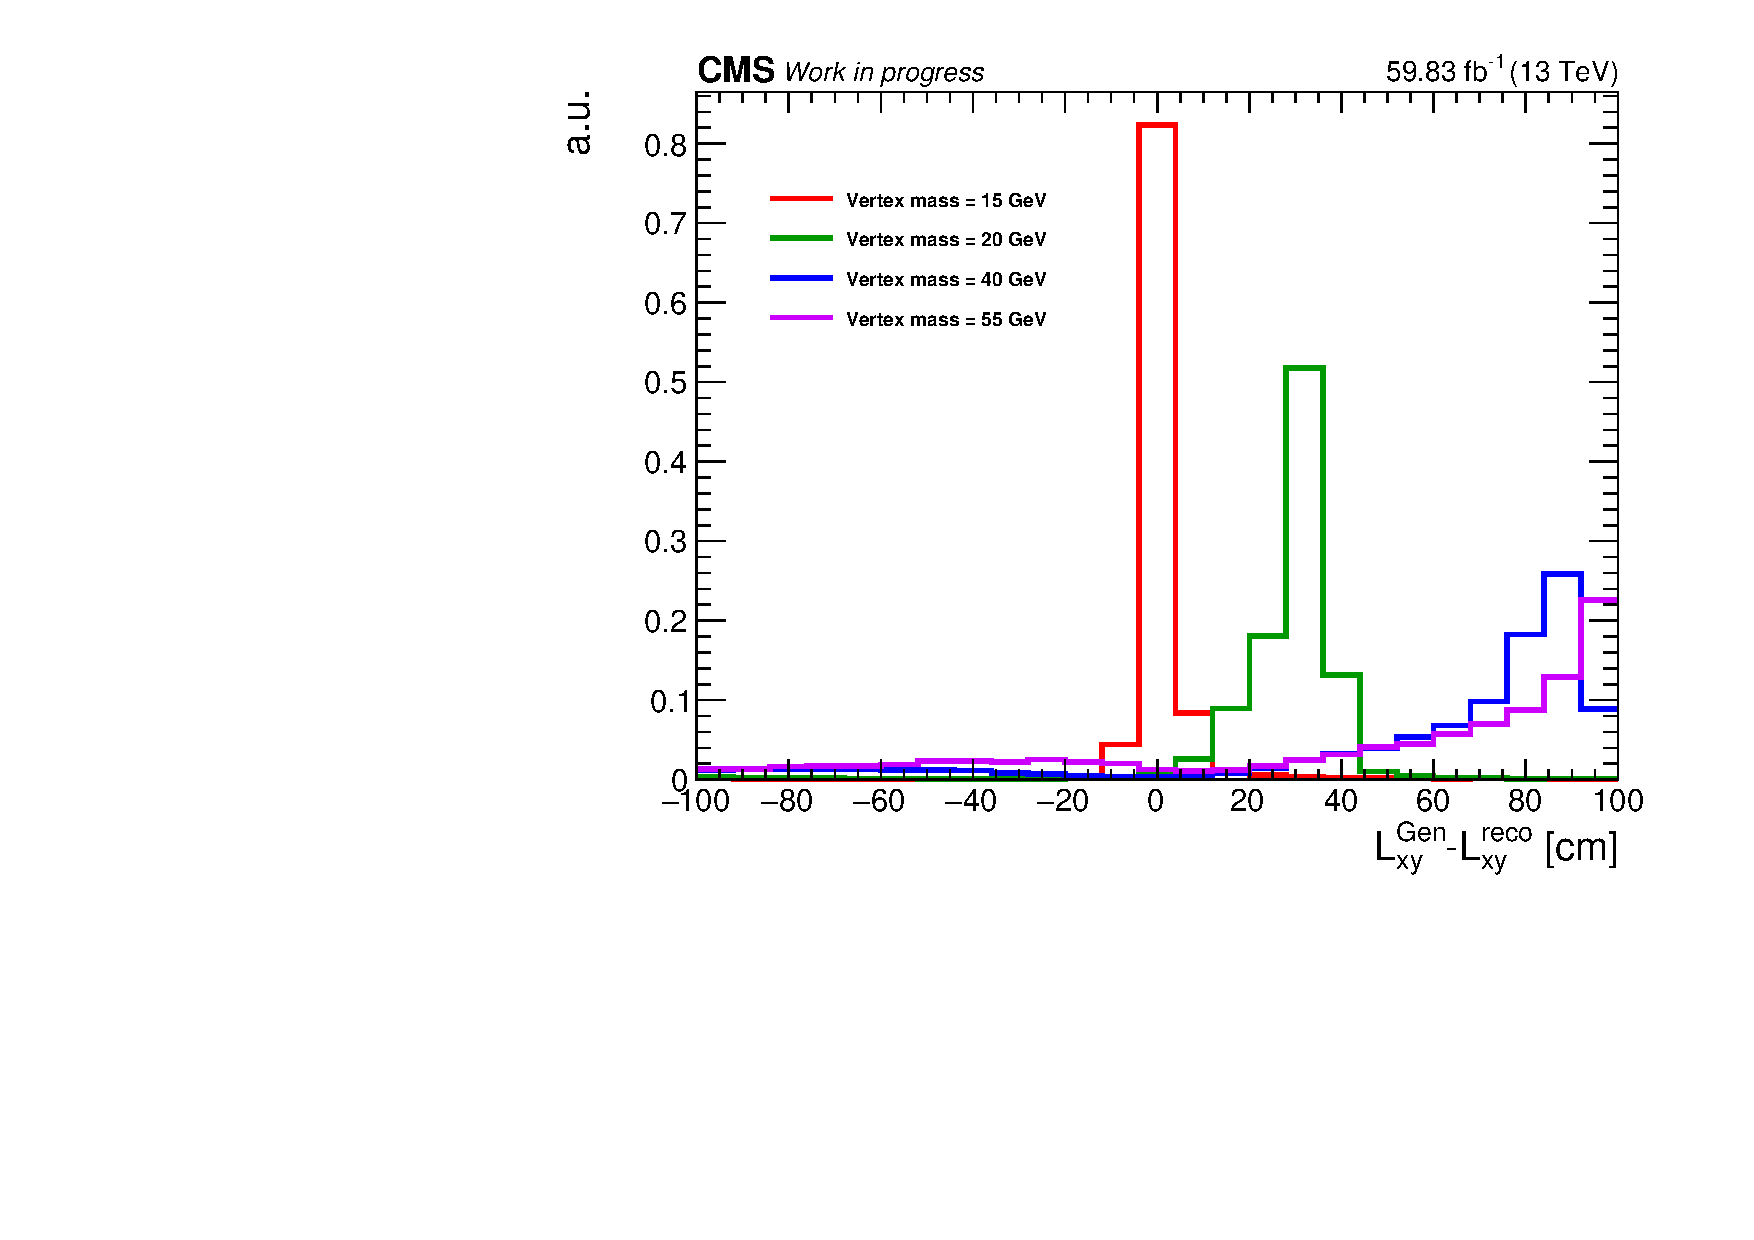
\includegraphics[width=\linewidth]{figs/05_analysis/2018_deltaLxy_Z_m15.pdf}
		\caption{$\mphi=15\GeV$}
	\end{subfigure}
	\begin{subfigure}[h]{0.45\linewidth}
		\centering
		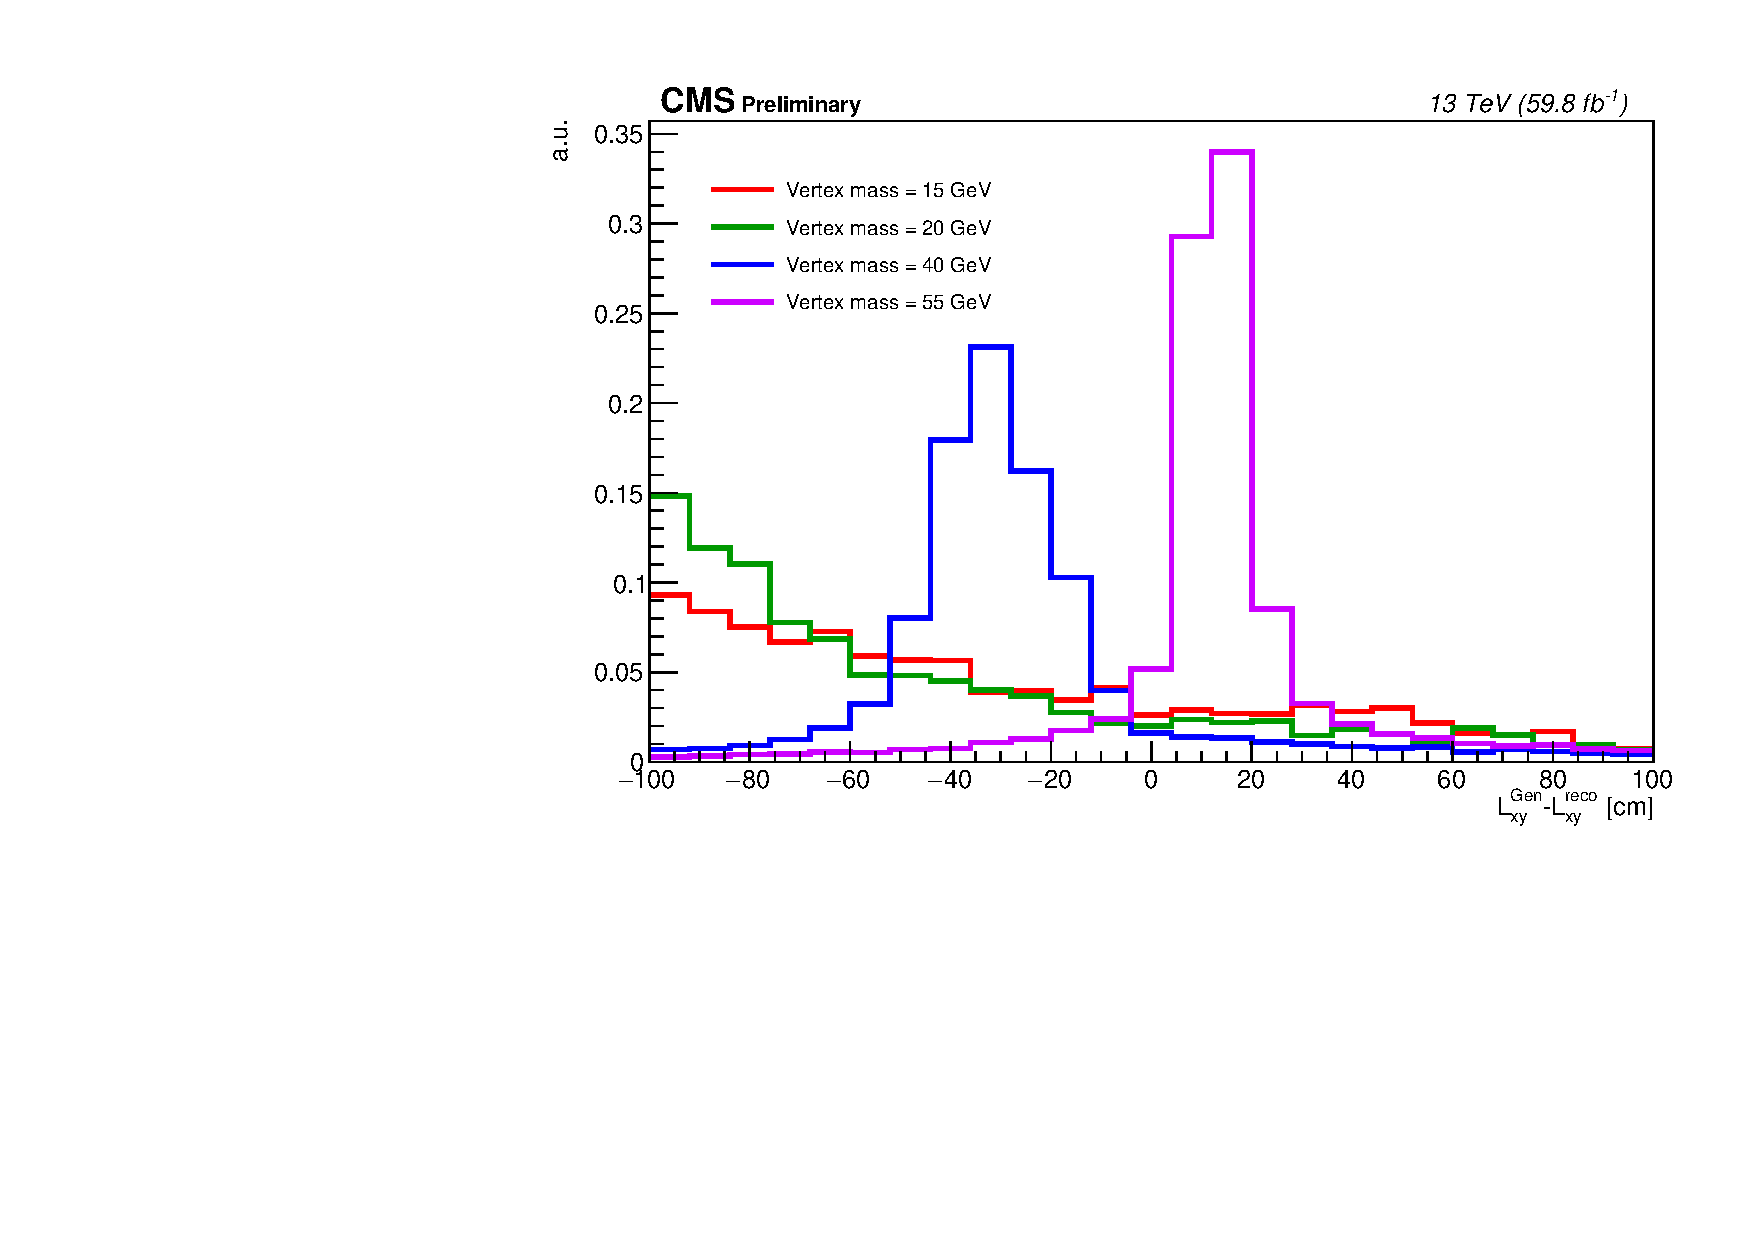
\includegraphics[width=\linewidth]{figs/05_analysis/2018_deltaLxy_Z_m50.pdf}
		\caption{$\mphi=50\GeV$}
	\end{subfigure}
	\caption[The difference between the true and reconstructed vertex grows as the assumed mass departs from the true one. Gen-reconstructed $\lxy$ for a \PZns+\PH samples under several assumed mass points.]{The difference between the true and reconstructed vertex grows as the assumed mass departs from the true one. Gen-reconstructed $\lxy$ for a \PZns+\PH samples under several assumed mass points.}
	\label{fig:deltaLxy}
\end{figure}

This analysis uses the \texttt{nanoAODv9} data format - the most compact data tier available for analysis use in CMS. As opposed to lower tier formats which contain detailed collections of classes to store event properties, nanoAOD provides only the most important information for high level physics objects~\cite{nanoaod}. This information includes several properties of photons but omits the calorimeter cluster position, which is required to calculate the diphoton vertex. To circumvent this, we propagate the photons from the PV to the ECAL using their $\eta$ and $\phi$. The ECAL is approximated using a cylinder with radius $\rho=137\unit{cm}$ and $z=324\unit{cm}$. These values were obtained using \texttt{miniAODv2} samples and are shown in figure~\ref{fig:calo_position}. Diphoton vertices calculated using the propagated coordinates yield a \lxy within 3\% of the \lxy calculations using the exact cluster coordinates, which is well within the intrinsic resolution of the vertex calculation.

\begin{figure}[htb!]
	\centering
	\captionsetup[subfigure]{justification=centering}
	\begin{subfigure}[h]{0.45\linewidth}
		\centering
		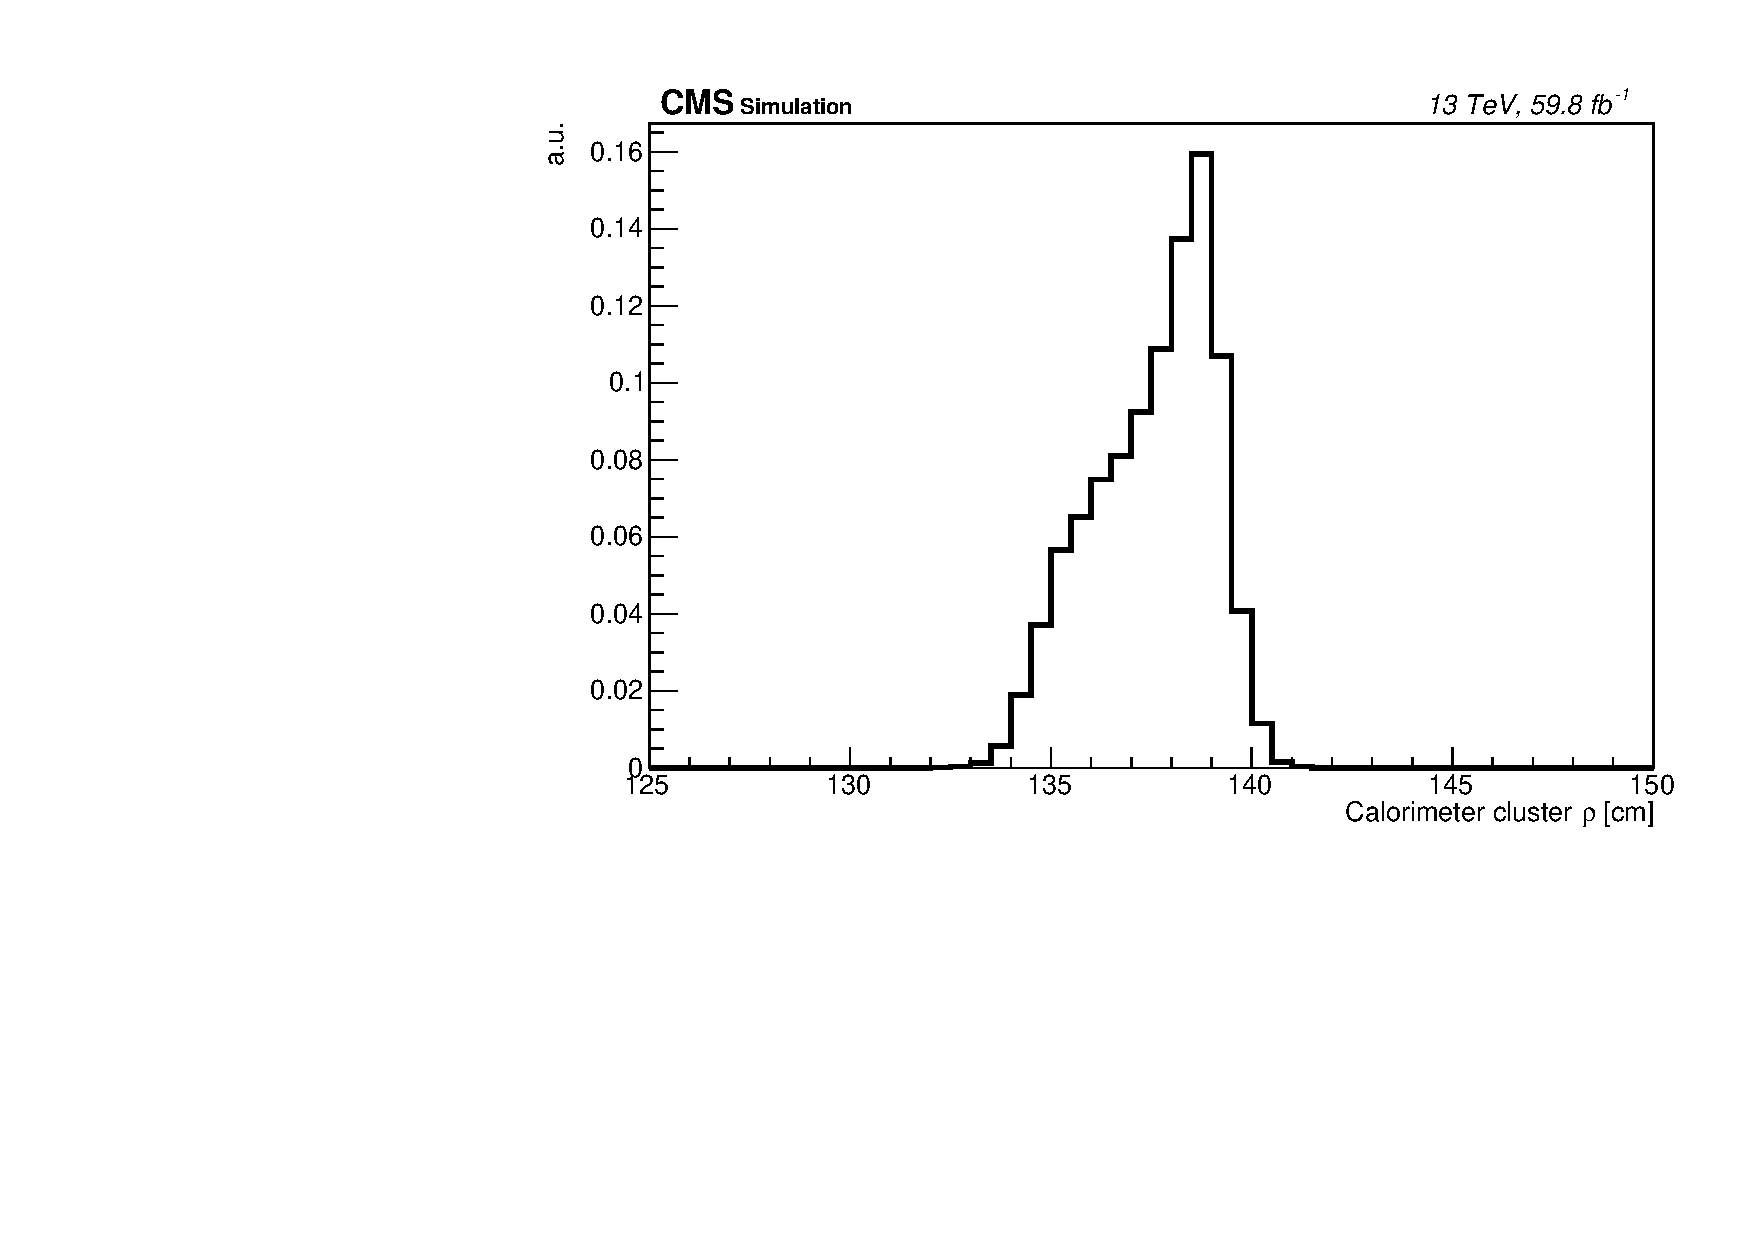
\includegraphics[width=\linewidth]{figs/05_analysis/calorimeter_rho.pdf}
		\caption{Calormieter cluster $\rho$}
	\end{subfigure}
	\begin{subfigure}[h]{0.45\linewidth}
		\centering
		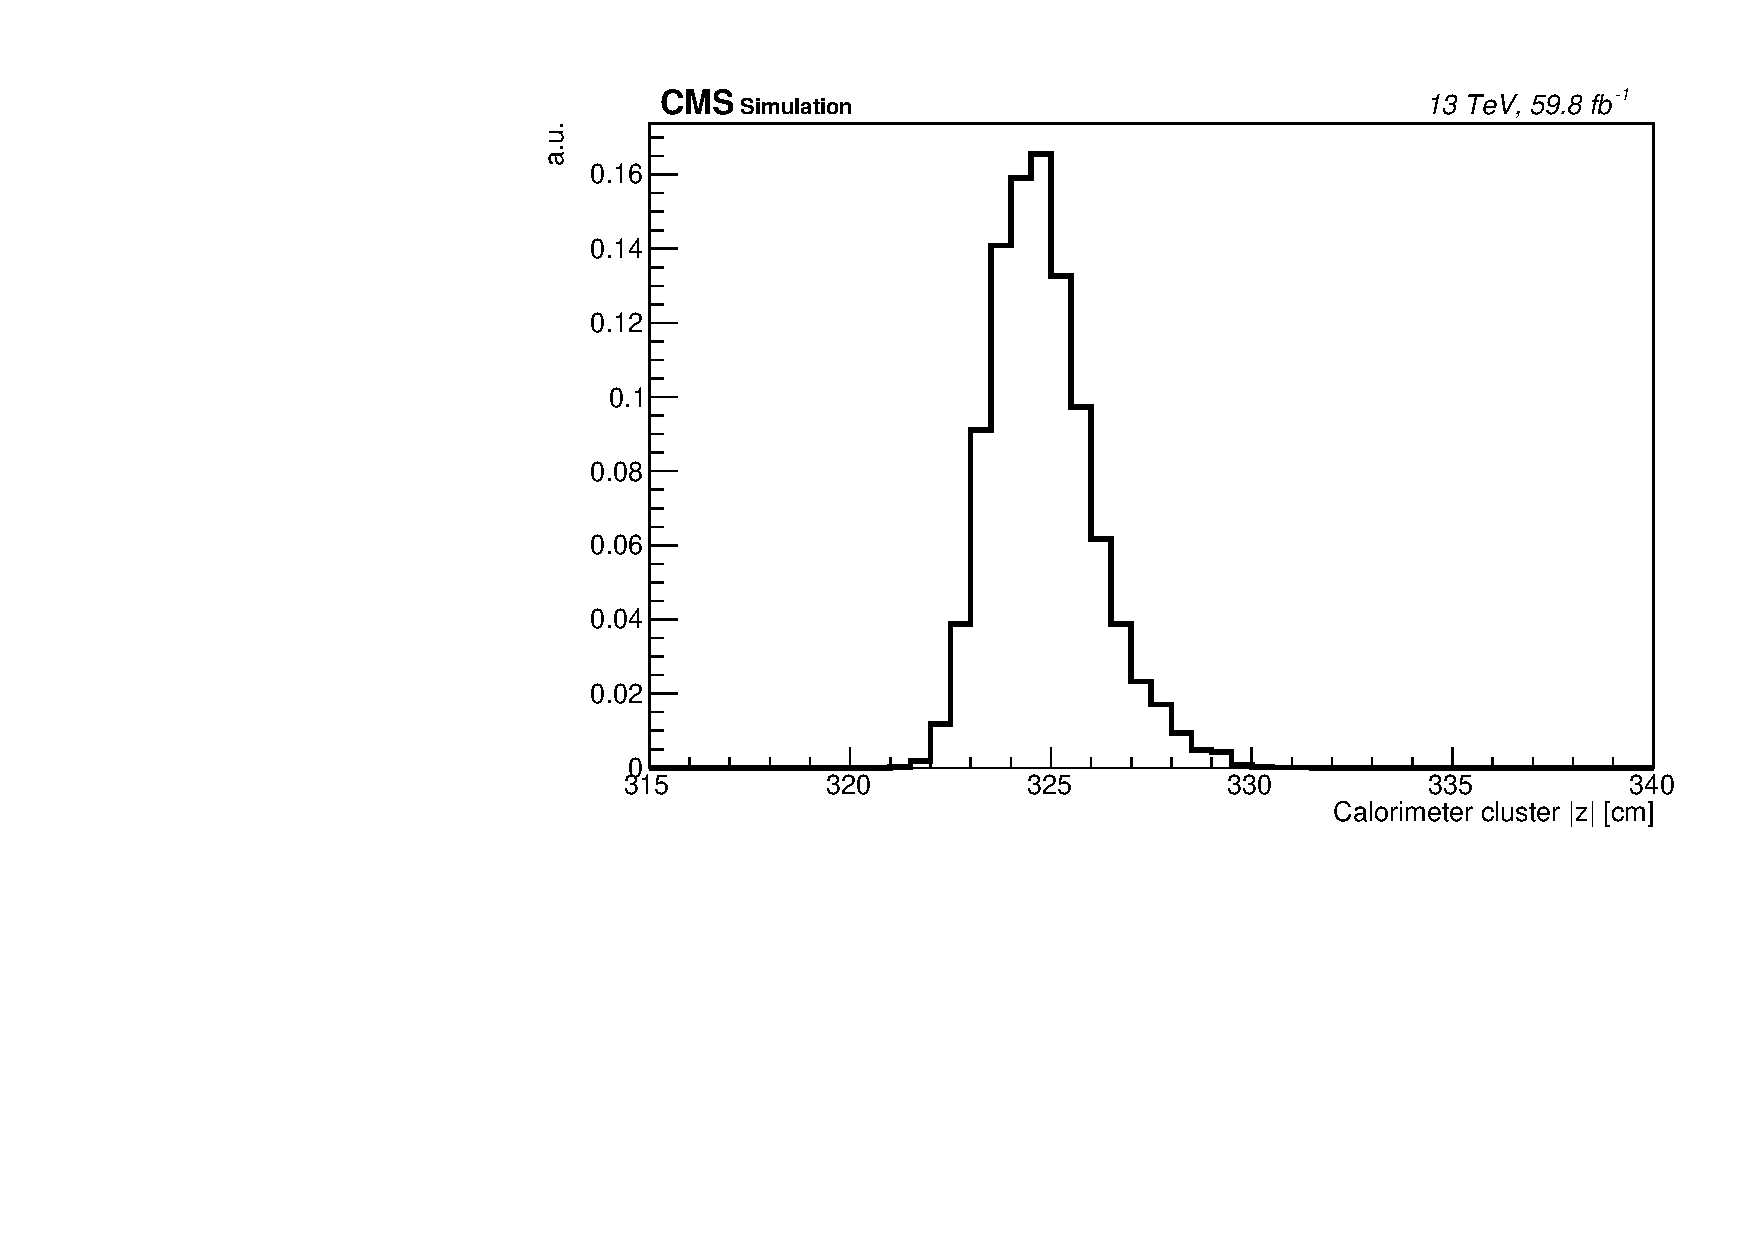
\includegraphics[width=\linewidth]{figs/05_analysis/calorimeter_z.pdf}
		\caption{Calorimeter cluster $|z|$}
	\end{subfigure}
	\caption{The $\rho$ for barrel photons and $|z|$ for endcap photons for all reconstructed photons using \texttt{miniAODv2} signal samples}
	\label{fig:calo_position}
\end{figure}

\section{Event Selection} \label{sec:ana_eventsel}
The first step in collecting events for the analysis is to select events passing HLT lepton triggers. Events passing these triggers are then chosen based on the presence of two same flavor, opposite charge leptons and two photons. Various quality cuts, referred to as preselection criteria, are applied to these objects to reject background. Lastly, event level cuts are applied to reject photons from final state radiation (FSR) and low \pt photons that get promoted to displaced $\Phi$ candidates by the kinematic vertex fit.

\subsection{Triggers} \label{sec:ana_triggers}
Events are triggered through leptonic decays of the \PZ boson produced in association with the SM Higgs Boson. The \PZ candidates are selected from dilepton events passing the HLT isolated single lepton triggers. These triggers are the standard lepton triggers recommended both the EGamma and Muon physics object groups (POGs) in CMS. Double lepton and high \pt lepton triggers were considered but provide only negligible improvement when applied in addition to the single lepton triggers. To ensure events are not double counted between data sets, muon events must pass the single muon triggers and are vetoed by the single electron triggers, while electron events must pass single electron triggers and are vetoed by the single muon triggers. A complete list of HLT trigger paths used for each year can be see in table~\ref{tab:triggers}.

\begin{table}[h]
	\caption[HLT trigger paths used for the Run 2 datasets]{HLT trigger paths used for the Run 2 datasets} 
	\label{tab:triggers}
	\begin{center}
		\begin{tabular}{l|l|l}\hline
			Year & Single Electron & Single Muon\\
			\hline
			2018 & HLT\_Ele32\_WPTight\_Gsf & HLT\_IsoMu24\\
			2017 & HLT\_Ele32\_WPTight\_Gsf & HLT\_IsoMu27\\
			2016 & HLT\_Ele27\_WPTight\_Gsf & HLT\_IsoMu24 \textbar\textbar HLT\_IsoTkMu24\\
			\hline
		\end{tabular}
	\end{center}
\end{table}

Each HLT path name corresponds to the different criteria required to pass the trigger. The electron triggers require the trigger object have $\pt>32\GeV$ ($27\GeV$ for 2016), pass tight selection criteria, and be reconstructed using the Gaussian sum filter (GSF) algorithm discussed in section~\ref{sec:CMS_reco_egamma}. Muons are required to pass isolation and have $\pt>24\GeV$ ($27\GeV$ for 2017). In order to improve the efficiency of the muon trigger in 2016, we also include the tracker muon trigger, which requires an isolated tracker muon with $\pt>24\GeV$.

\subsection{Preselection Criteria} \label{sec:ana_preselection}
For both electrons and muons we define a set of tight and loose leptons based on cut based ID set by the EGamma and Muon POGs. To reconstruct a \PZ candidate, we require exactly two same flavor opposite charge tight leptons with invariant mass $70<m_{\ell\ell}<110\GeV$ and zero additional loose leptons. For photons we require at least two photons passing a set of preselection criteria, which are subject to additional classification based on cut based ID.

\subsubsection{Particle Flow Isolation} \label{sec:ana_isolation}
One key application of the particle flow (PF) algorithm is the calculation of a particle's isolation. This quantity measures the \pt and energy contributions from PF candidates in a fixed $\Delta R$ cone centered on the original particle. A lower value implies the particle is more isolated (i.e. there are fewer additional particles nearby), and vice versa. Isolation is a key variable to reject particles produced in jets from heavy-flavor hadronic decays or decays of pions and kaons~\cite{Sirunyan:PF}. A particle's isolation is defined as follows:
\begin{equation}
	\label{eq:pfiso}
	I_\text{pf} = \sum_{\substack{i\in\text{charged}\\\text{hadrons}}}\pt^i+\text{max}\left(0,\sum_{\substack{i\in\text{neutral}\\\text{hadrons}}}\et^i+\sum_{\gamma\in\text{photons}}\et^\gamma-\text{PU Corrections}\right)
\end{equation}

The three contributions that are summed over in equation~\ref{eq:pfiso} are referred to as charged hadron isolation ($I_\text{ch}$), neutral hadron isolation ($I_\text{n}$), and photon isolation ($I_\gamma$). It is also common to refer to a particle's isolation normalized by its \pt (or $E_\mathrm{T}$ for neutral particles), known as relative isolation which is defined as
\begin{equation}
	\label{eq:reliso}
	I_\text{rel}=\frac{I_\text{pf}}{\pt}
\end{equation}

Particles created from pileup can create calorimeter deposits within the $\Delta R$ cone used to calculate isolation. These are unrelated to the physics process for the central particle and can artificially inflate the isolation. Only charged hadrons with tracks originating from the PV are used when calculating the charged hadron isolation, which rejects charged hadrons originating from PU. Neutral particles, however, do not produce tracks, meaning calorimeter deposits from the PV and from pileup are indistinguishable. Because of this, there are additional corrections to remove the PU contributions from neutral hadron and photon isolation. Two common methods are $\rho$ corrections, which calculate the average energy density per unit area from pileup ($\rho$) multiplied by an effective area as a function of $\eta$, and $\Delta\beta$ corrections, which calculate the energy from photons and neutral hadrons in pileup as a fraction of the charged hadron contribution from PU.

\subsubsection{Muon Criteria} \label{sec:ana_muons}
The NanoAOD data format takes reconstructed muons and applies loose cuts before storing the muon properties. These branches contain all muons with $\pt>3\GeV$ with minimal cuts to reconstruction quality. For the purpose of this analysis, muons are classified as loose if they pass all of the following criteria:
\begin{itemize}
	\item $\pt>10\GeV$
	\item $|\eta|<2.4$
	\item $D_{xy}<0.2\unit{cm}$: the transverse distance from the PV to the beamline must be less than 0.2 cm
	\item $D_{z}<0.5\unit{cm}$: the longitudinal distance from the PV to the beamline must be less than 0.5 cm
	\item $I_\text{rel}(\Delta R<0.4,\,\Delta\beta\text{-corrected})<0.25$
	\item Passes loose quality criteria set by the Muon POG:
	\begin{itemize}
		\item Muon must be reconstructed by the PF algorithm
		\item Muon must be either a global and/or tracker muon
	\end{itemize}
\end{itemize}
We define tight muons as a subset of loose muons if they pass the following criteria:
\begin{itemize}
	\item $I_\text{rel}(\Delta R<0.4,\,\Delta\beta\text{-corrected})<0.15$
	\item Passes tight quality criteria set by the Muon POG:
	\begin{itemize}
		\item Muon must be a global muon
		\item The global muon track fit must have $\chi^2/\text{ndof}<10$
		\item Global track must have at least one hit in a muon chamber %TODO: why is this necessary if it's already a global muon?
		\item Muon track must have segments in at least 2 different muon stations %TODO: same question
		\item Tracker track $D_{xy}<2\unit{mm}$
		\item Tracker track $D_{z}<5\unit{mm}$
		\item Tracker track must have at least 1 hit in the pixel detector
		\item Tracker track must have hits in more than 5 tracker layers
	\end{itemize}
\end{itemize}
We also require that one of the two tight muons used to reconstruct the \PZ be the triggering muon, and that the triggering muon have $\pt>25\GeV$ ($28\GeV$ in 2017) in order to operate above the single muon trigger \pt thresholds.

\subsubsection{Electron Criteria} \label{sec:ana_electrons}
Analogously to the muon criteria, loose electrons are defined from reconstructed electrons if they pass a set of preselection criteria. 
\begin{itemize}
	\item $\pt>15\GeV$
	\item $|\eta|<2.4$
	\item $|\eta|>1.57\text{ or }|\eta|<1.44$ to rejects clusters in the overlap region between the ECAL barrel and endcap
	\item $D_{xy}<0.2\unit{cm}$, $D_{z}<0.2\unit{cm}$
	\item Passes cut based ID provided by the EGamma POG at the \texttt{veto} working point
\end{itemize}
Tight electrons are selected from this collection of they pass cut based ID at the \texttt{tight} working point set by the EGamma POG. A full set of criteria is shown in table~\ref{tab:electronID} for barrel and endcap electrons. Similar to the muon criteria, we require one of the tight electrons be the triggering electron, and that the triggering electron have $\pt>35\GeV$.

\begin{table}[htb!]
	\centering
	\caption[Cut based ID selection criteria for electrons in Run-2~\cite{electronid}.]{Cut based ID selection criteria for electrons in Run-2~\cite{electronid}.}
	\label{tab:electronID}
	\subcaption{Barrel Electrons}
	\begin{tabular}{l | r | r}
		\hline
		Barrel Criteria & Veto & Tight \\
		\hline
		\hline
		$\sigma_{i\eta i\eta}<$ & 0.0126 & 0.0104 \\
		$|\Delta\eta_\text{seed}|<$ & 0.0463 & 0.00255 \\
		$|\Delta\phi_\text{In}|<$ & 0.148 & 0.022 \\
		$H/E<$ & $0.05+1.16/E+0.0324\rho/E$ & $0.026+1.15/E+0.0324\rho/E$ \\
		$I_\text{rel}(\Delta R<0.3,\rho\text{ corrected})<$ & $0.198+0.506/\pt$ & $0.0287+0.506/\pt$\\
		$|1/E-1/p|<$  & 0.209 & 0.159 \\
		Missing inner hits $\leq$ & 2 & 1 \\
		Passes conversion veto & True & True\\
		\hline
	\end{tabular}
	\centering
	%\caption[Cut based ID selection criteria for endcap electrons in Run-2~\cite{electronid}]{Cut based ID selection criteria for endcap electrons in Run-2~\cite{electronid}}
	%\label{tab:electron_endcap}
	\subcaption{Endcap Electrons}
	\begin{tabular}{l | r | r}
		\hline
		Endcap Criteria & Veto & Tight \\
		\hline
		\hline
		$\sigma_{i\eta i\eta}<$ & 0.0457 & 0.0353 \\
		$|\Delta\eta_\text{seed}|<$ & 0.00814 & 0.00501 \\
		$|\Delta\phi_\text{In}|<$ & 0.19 & 0.0236 \\
		$H/E<$ & $0.05+2.54/E+0.183\rho/E$ & $0.0188+2.06/E+0.183\rho/E$ \\
		$I_\text{rel}(\Delta R<0.3,\rho\text{ corrected})<$ & $0.203+0.963/\pt$ & $0.0445+0.963/\pt$\\
		$|1/E-1/p|<$ & 0.132 & 0.0197 \\
		Missing inner hits $\leq$ & 3 & 1 \\
		Passes conversion veto & True & True\\
		\hline
	\end{tabular}
\end{table}

The variables used in the cut based ID are optimized to reject background such as photons in hadronic showers or photons that convert to $e^+e^-$ pairs in the tracker. The spread of the calorimeter cluster in $\eta$ is measured using $\sigma_{i\eta i\eta}$, which is the weighted second moment of the cluster shape in $\eta$ measured in a $5\times5$ grid of calorimeter crystals, centered on the most energetic crystal in the SC. This variable can be used to discriminate two photon showers produced from neutral meson decays, which have higher spread in $\eta$, from showers produced by prompt electrons or photons. The $H/E$ ratio takes the energy of HCAL clusters located in a $\Delta R<0.15$ cone behind the ECAL cluster and divides it by the ECAL cluster energy. Genuine EM showers have three main contributions to hadronic energy: leakage through gaps into the HCAL, calorimeter noise, and pileup. The constant term in these cuts accounts for energy leakage from real electrons or photons, the term proportional to $1/E$ is to account for noise in the HCAL, and the $\rho/E$ term is the correction due to pileup. Tracker information is also used to separate signal from background. The $|\Delta\eta_\text{seed}|$ and $|\Delta\phi_\text{in}|$ are the difference in SC and track $\eta$/$\phi$, measured from the innermost tracker layer, which is expected to be small for prompt electrons. The difference between tracker momentum and calorimeter energy is measured using the quantity $|1/E-1/p|$, which should be small as a good electron should have similar energy and momentum. The number of missing hits refers to number of gaps in the electron's trajectory through the tracker. Converted photons will leave tracks after the conversion vertex but leave no hits in the tracker before they convert, while prompt electrons should leave hits in the tracker starting from the PV. An additional conversion veto is applied by rejecting electrons with tracks matched to conversion vertices in order to further reject background from converted photons. The tight cut based ID is expected to have a 70\% signal efficiency for real electrons.

\subsubsection{Photon Criteria} \label{sec:ana_photons}
Reconstructed photons must pass baseline selection to be included in the nanoAOD data format. All nanoAOD photons must have $\pt>5\GeV$, $R_9>0.8$, and pass cuts on total and relative charged hadron isolation given by $I_\text{ch}<20\GeV$ and $I_\text{ch}/\pt<0.3$. The $R_9$ of a supercluster is defined as the energy the most energetic $3\times3$ crystal grid in the supercluster divided by the total supercluster energy. For an event to be considered for this analysis, we require at least two nanoAOD photons passing the following preselection criteria:
\begin{itemize}
	\item $\pt>20\GeV$
	\item Passes pixel seed veto
	\item $|\eta|<2.4$
	\item $|\eta|>1.57\text{ or }|\eta|<1.44$
	\item $\Delta\eta$($\gamma$, lepton)$^2$/0.4$^2$ + $\Delta\varphi$($\gamma$, lepton)$^2$/0.5$^2$ $>$ 1 for all loose leptons
\end{itemize}

Due to the production mechanism of the Higgs boson, the $\Phi$ and subsequent photon pair are expected to be strongly correlated and have high energy. The following kinematic requirements based on the four-momentum of the diphoton system reject background due to uncorrelated or lower energy photon pairs while maintaining 99\% signal efficiency:
\begin{itemize}
	\item $\pt(\gamma,\gamma)>20\GeV$
	\item Invariant diphoton mass $\mgg>4\GeV$
\end{itemize}

The pixel seed veto reject photons if there are at least two pixel seed hits that point to the supercluster, which is used to reject background from electrons that are misidentified as photons. Photons passing this preselection criteria are subject to further classification as ID'd or anti-ID'd if they pass or fail loose cut based ID outlined in table~\ref{tab:photonID}. The loose ID is measured to have approximately 90\% efficiency for prompt photons, but was observed to have additional inefficiencies due to photon isolation and shower shape variables resulting from the displaced signature of the two photons. As the photon vertex becomes more displaced, the shower shape becomes more skewed and the two photons become closer together, which affects the cuts to $\sigma_{i\eta i\eta}$ and $I_\gamma$. At lower masses, the photon isolation is the main source of inefficiency because the photons are more collimated, while at higher masses the $\sigma_{i\eta i\eta}$ is the main inefficiency as the larger angle between the photons causes a larger spread in shower shape. The effect of each criteria in the cut based ID on the photon reconstruction efficiency is shown as a function of generator level \lxy in figure~\ref{fig:Photon_cutBased} for all values of \mphi. The efficiency denominator is all generator level (gen) photon pairs, where each gen photon has $\pt>20\GeV$ and a decay vertex within the CMS ECAL. The numerator requires each gen photon to have a matching reconstructed photon that passes given selection criteria. Matching requires the reconstructed photon have $\Delta R < 0.3$ and energy within 50\% of the gen photon.

Given the large inefficiency of the $I_\gamma$ cuts at low values of $\mphi$, studies were performed using modified photon isolation by removing the footprint of the partner photon from $I_\gamma$. This modified ID showed up to 50\% improvement in signal efficiency for low \mphi, high \lxy events. However, this was shown to introduce substantial irreducible background with only marginal improvements to expected limits, so it was not used in the final analysis.

\begin{table}[htb!]
	\centering
	\caption[Cut based ID selection criteria for photons in Run-2~\cite{photonid}.]{Cut based ID selection criteria for photons in Run-2~\cite{photonid}.}
	\label{tab:photonID}
	\begin{tabular}{l | l}
		\hline
		Barrel Criteria & Loose ID \\
		\hline
		\hline
		$H/E<$ & 0.04596\\
		$\sigma_{i\eta i\eta}<$ & 0.0106\\
		$I_\text{ch}(\Delta R<0.3,\rho\text{ corrected})<$ & 1.694\\
		$I_\text{n}(\Delta R<0.3,\rho\text{ corrected})<$ & $24.032+0.01512*\pt+2.259*10^{-5}*\pt^2$\\
		$I_\gamma(\Delta R<0.3,\rho\text{ corrected})<$ & $2.876+0.004017*\pt$\\
		\hline
		\multicolumn{2}{l}{}\\
		\hline
		Endcap Criteria & Loose ID \\
		\hline
		\hline
		$H/E<$ & 0.0590\\
		$\sigma_{i\eta i\eta}<$ & 0.0272\\
		$I_\text{ch}(\Delta R<0.3,\rho\text{ corrected})<$ & 2.089\\
		$I_\text{n}(\Delta R<0.3,\rho\text{ corrected})<$ & $19.722+0.01512*\pt+2.3*10^{-5}*\pt^2$\\
		$I_\gamma(\Delta R<0.3,\rho\text{ corrected})<$ & $4.162+0.0037*\pt$\\
		\hline
	\end{tabular}
\end{table}

\begin{figure}[htb!]
	\centering
	\begin{tabular}{>{\centering\arraybackslash}m{0.32\linewidth} >{\centering\arraybackslash}m{0.32\linewidth} >{\centering\arraybackslash}m{0.32\linewidth}}
		$\mphi=15\GeV$ & $\mphi=20\GeV$ & $\mphi=30\GeV$ \\
		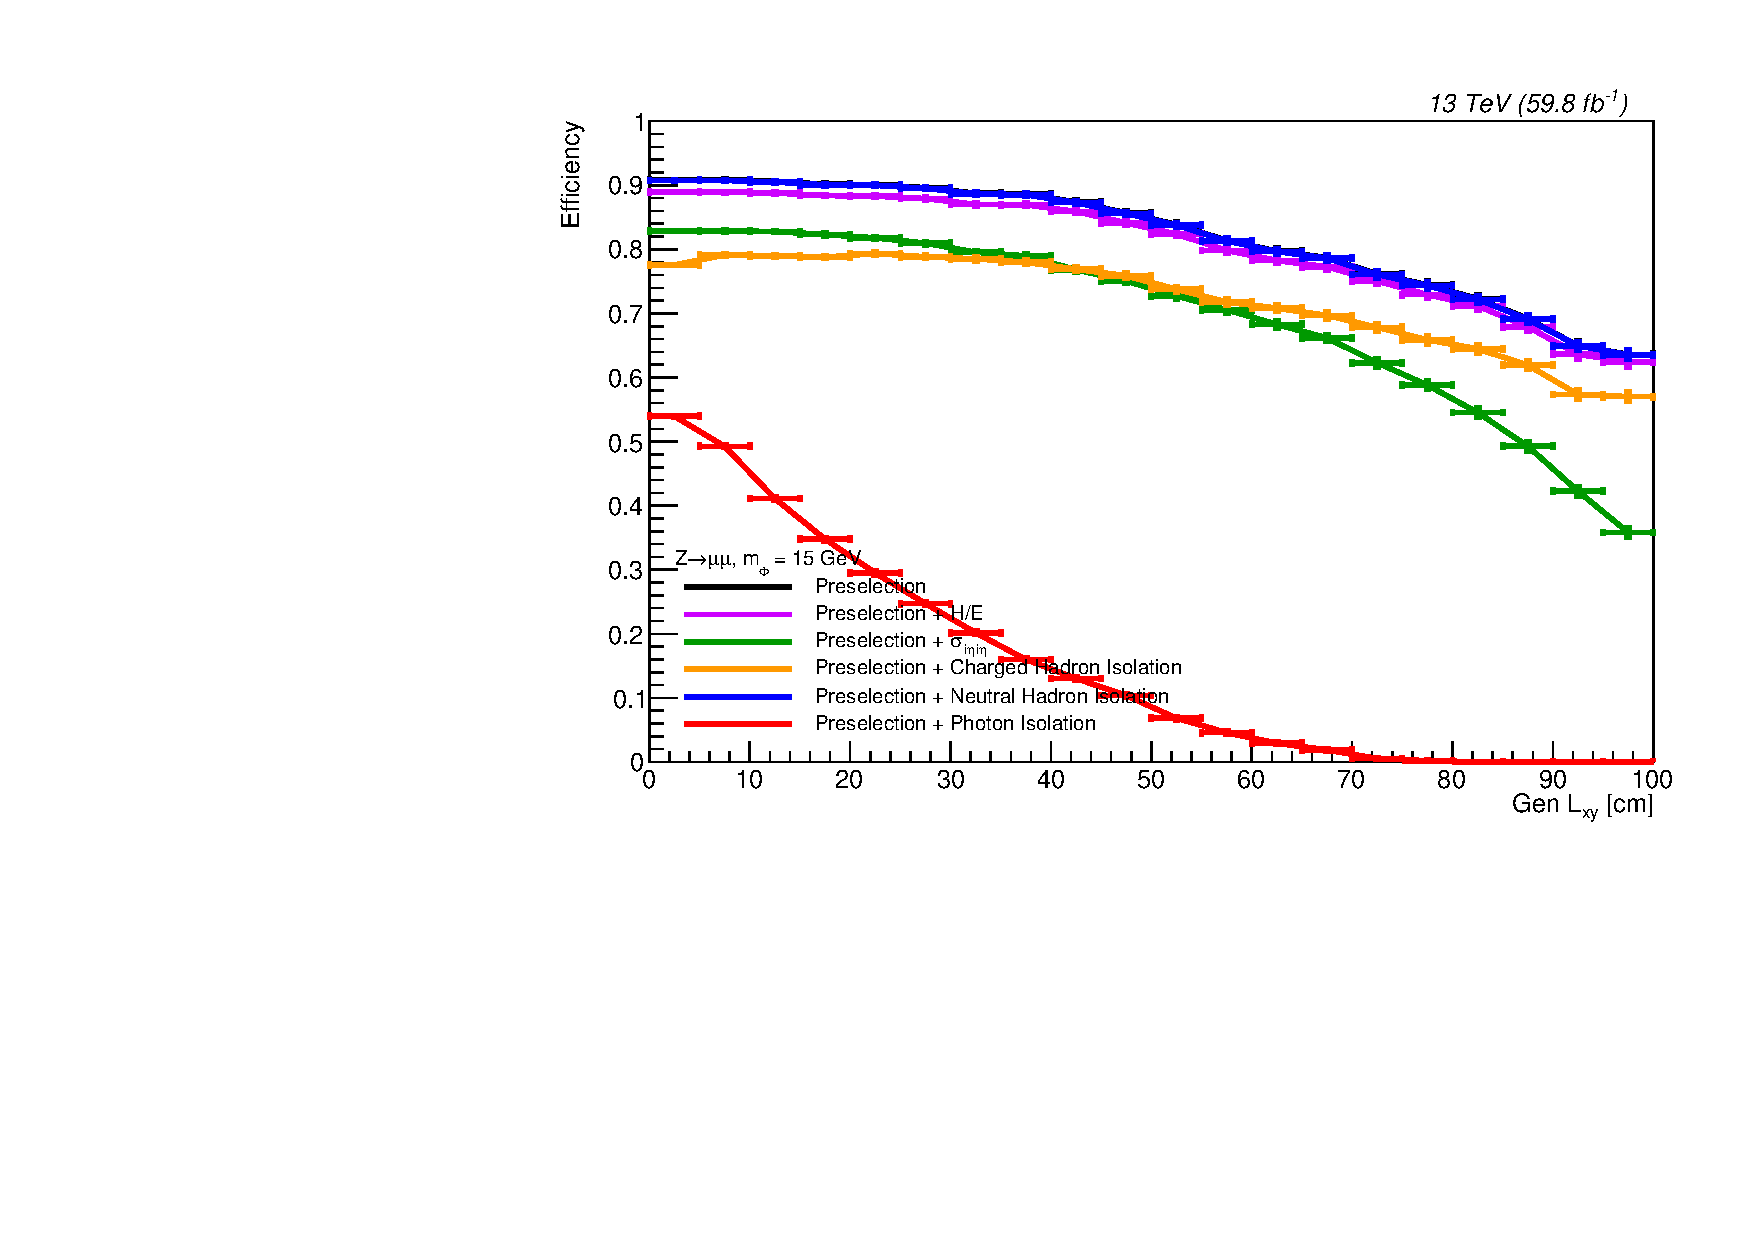
\includegraphics[width=\linewidth]{figs/05_analysis/cutBasedID_effVsLxy_Z_m15_cats_2018.pdf} &
		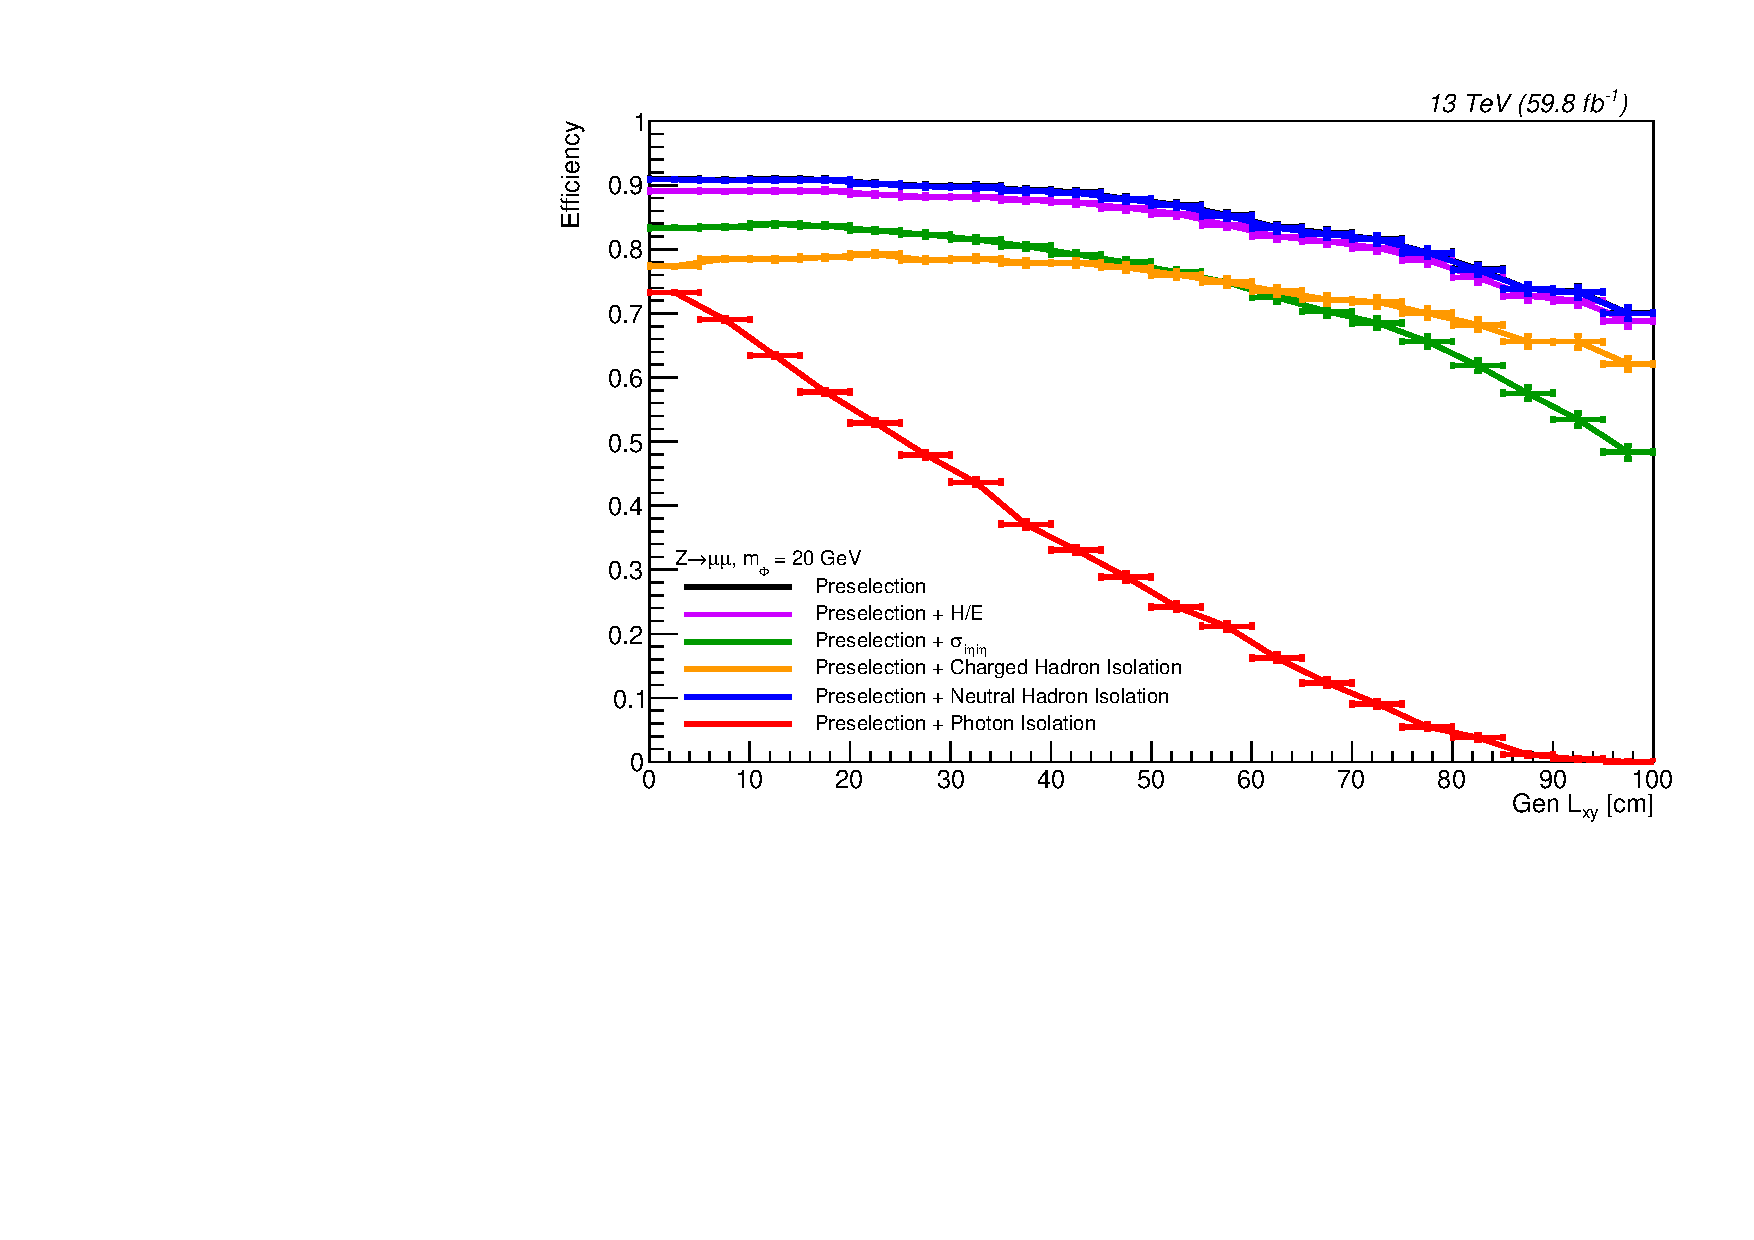
\includegraphics[width=\linewidth]{figs/05_analysis/cutBasedID_effVsLxy_Z_m20_cats_2018.pdf} &
		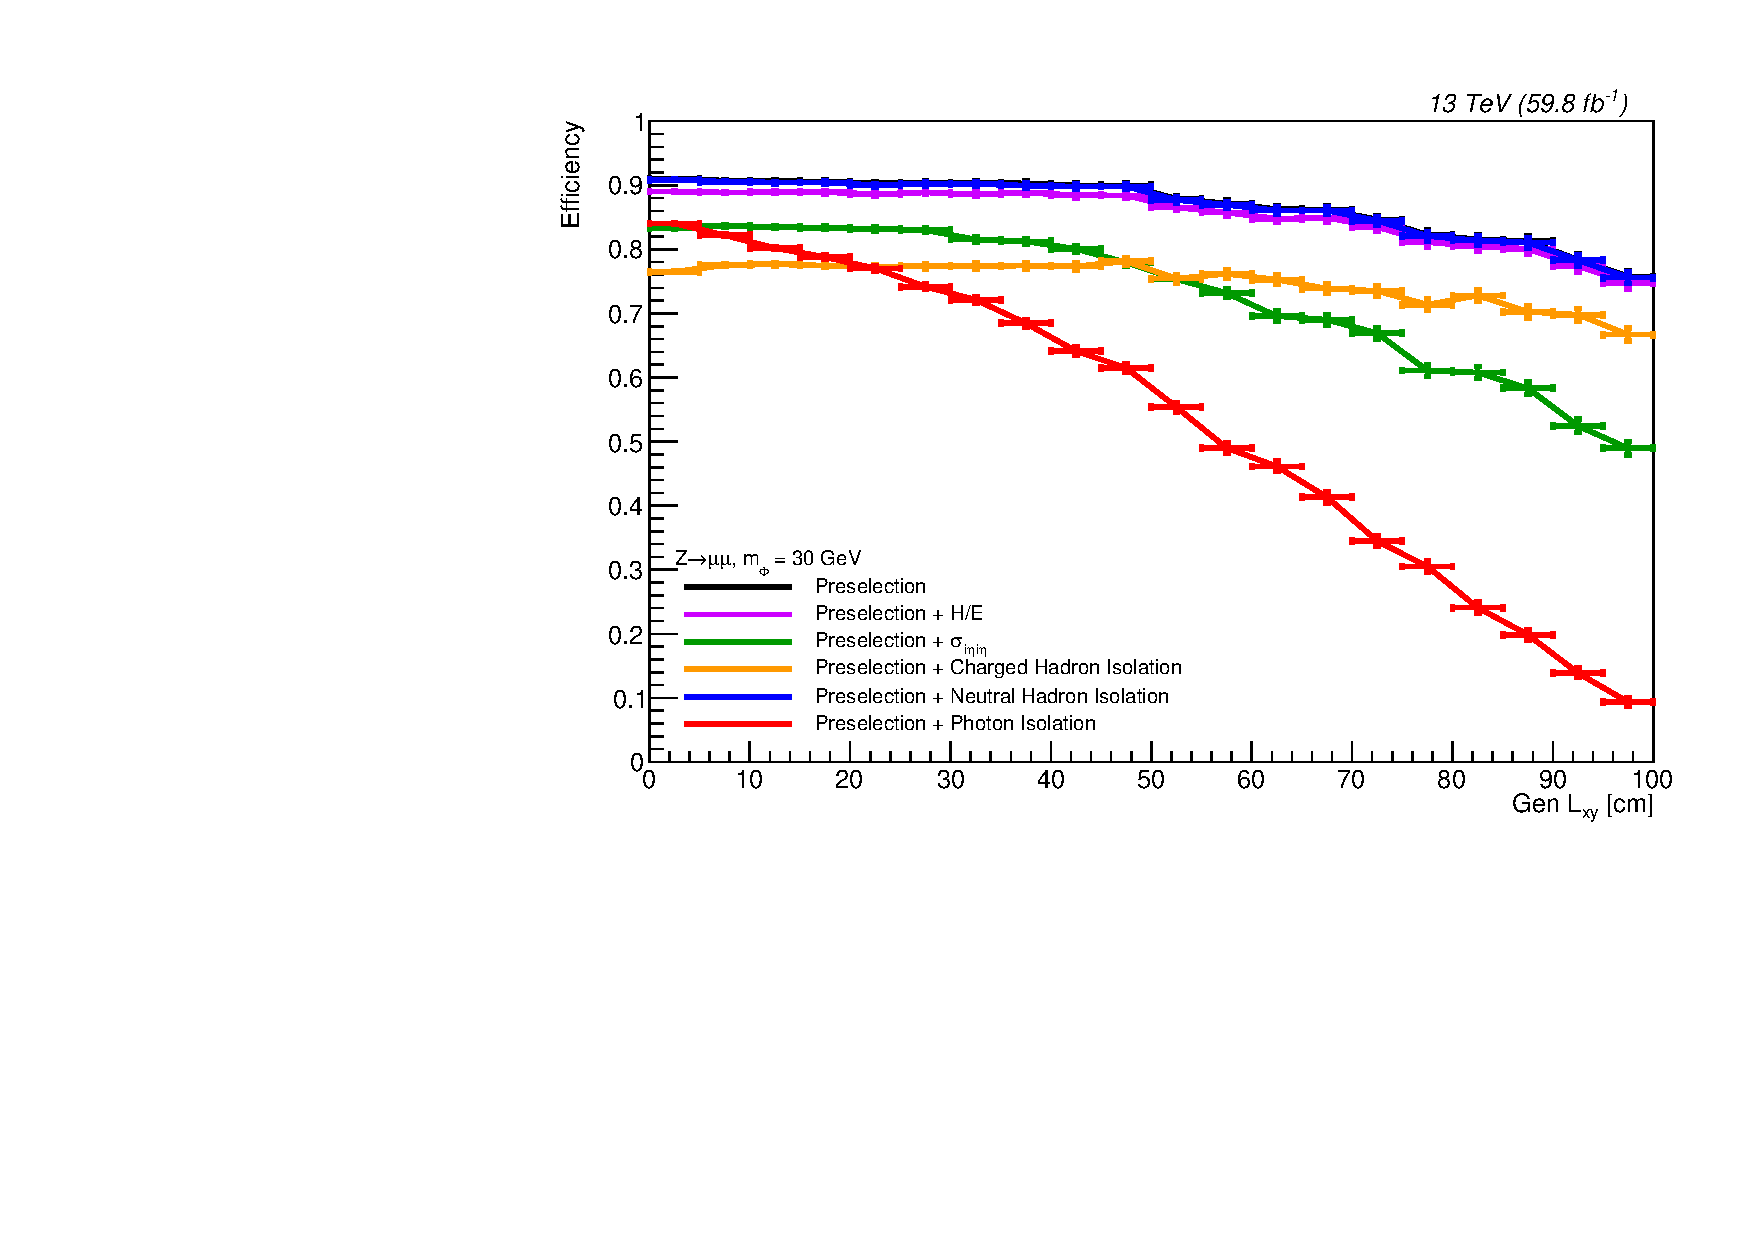
\includegraphics[width=\linewidth]{figs/05_analysis/cutBasedID_effVsLxy_Z_m30_cats_2018.pdf} \\
		$\mphi=40\GeV$ & $\mphi=50\GeV$ & $\mphi=55\GeV$ \\
		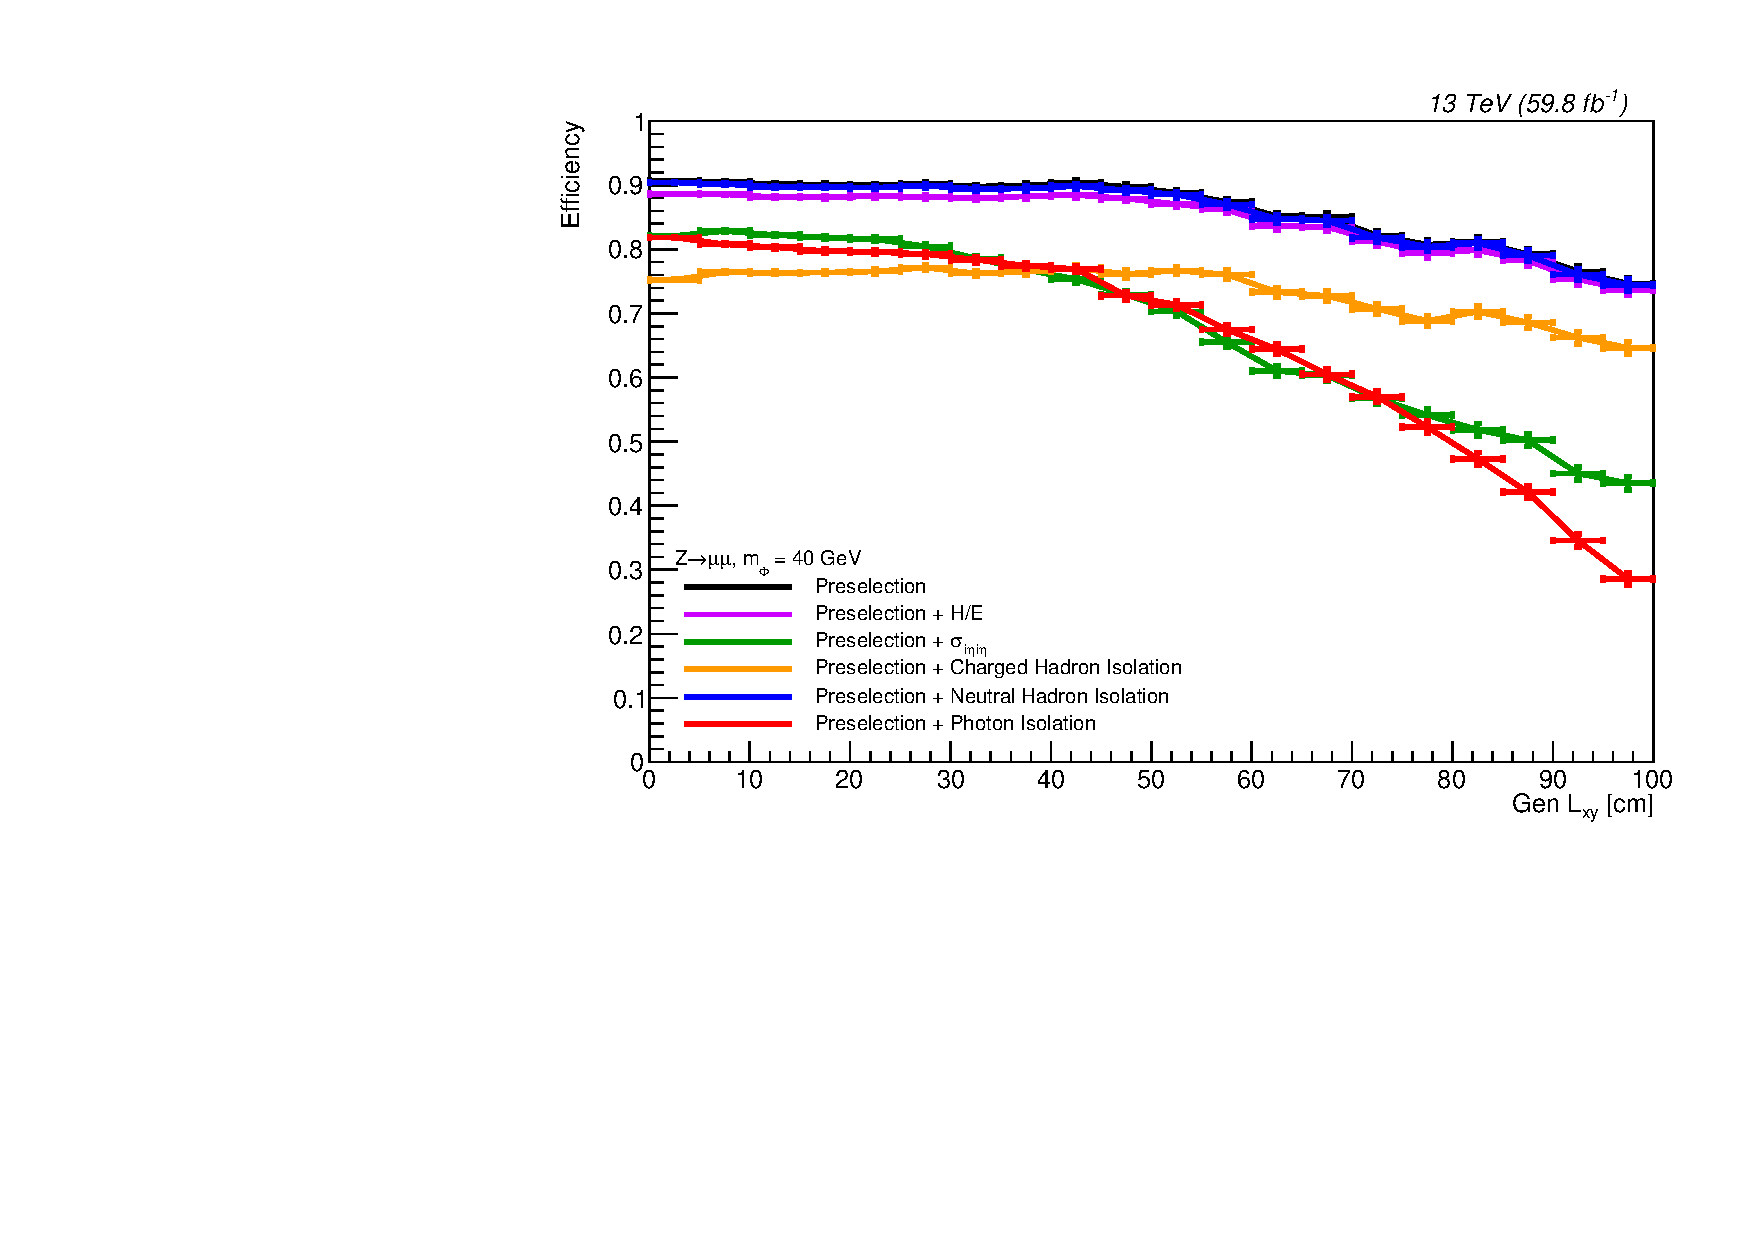
\includegraphics[width=\linewidth]{figs/05_analysis/cutBasedID_effVsLxy_Z_m40_cats_2018.pdf} &
		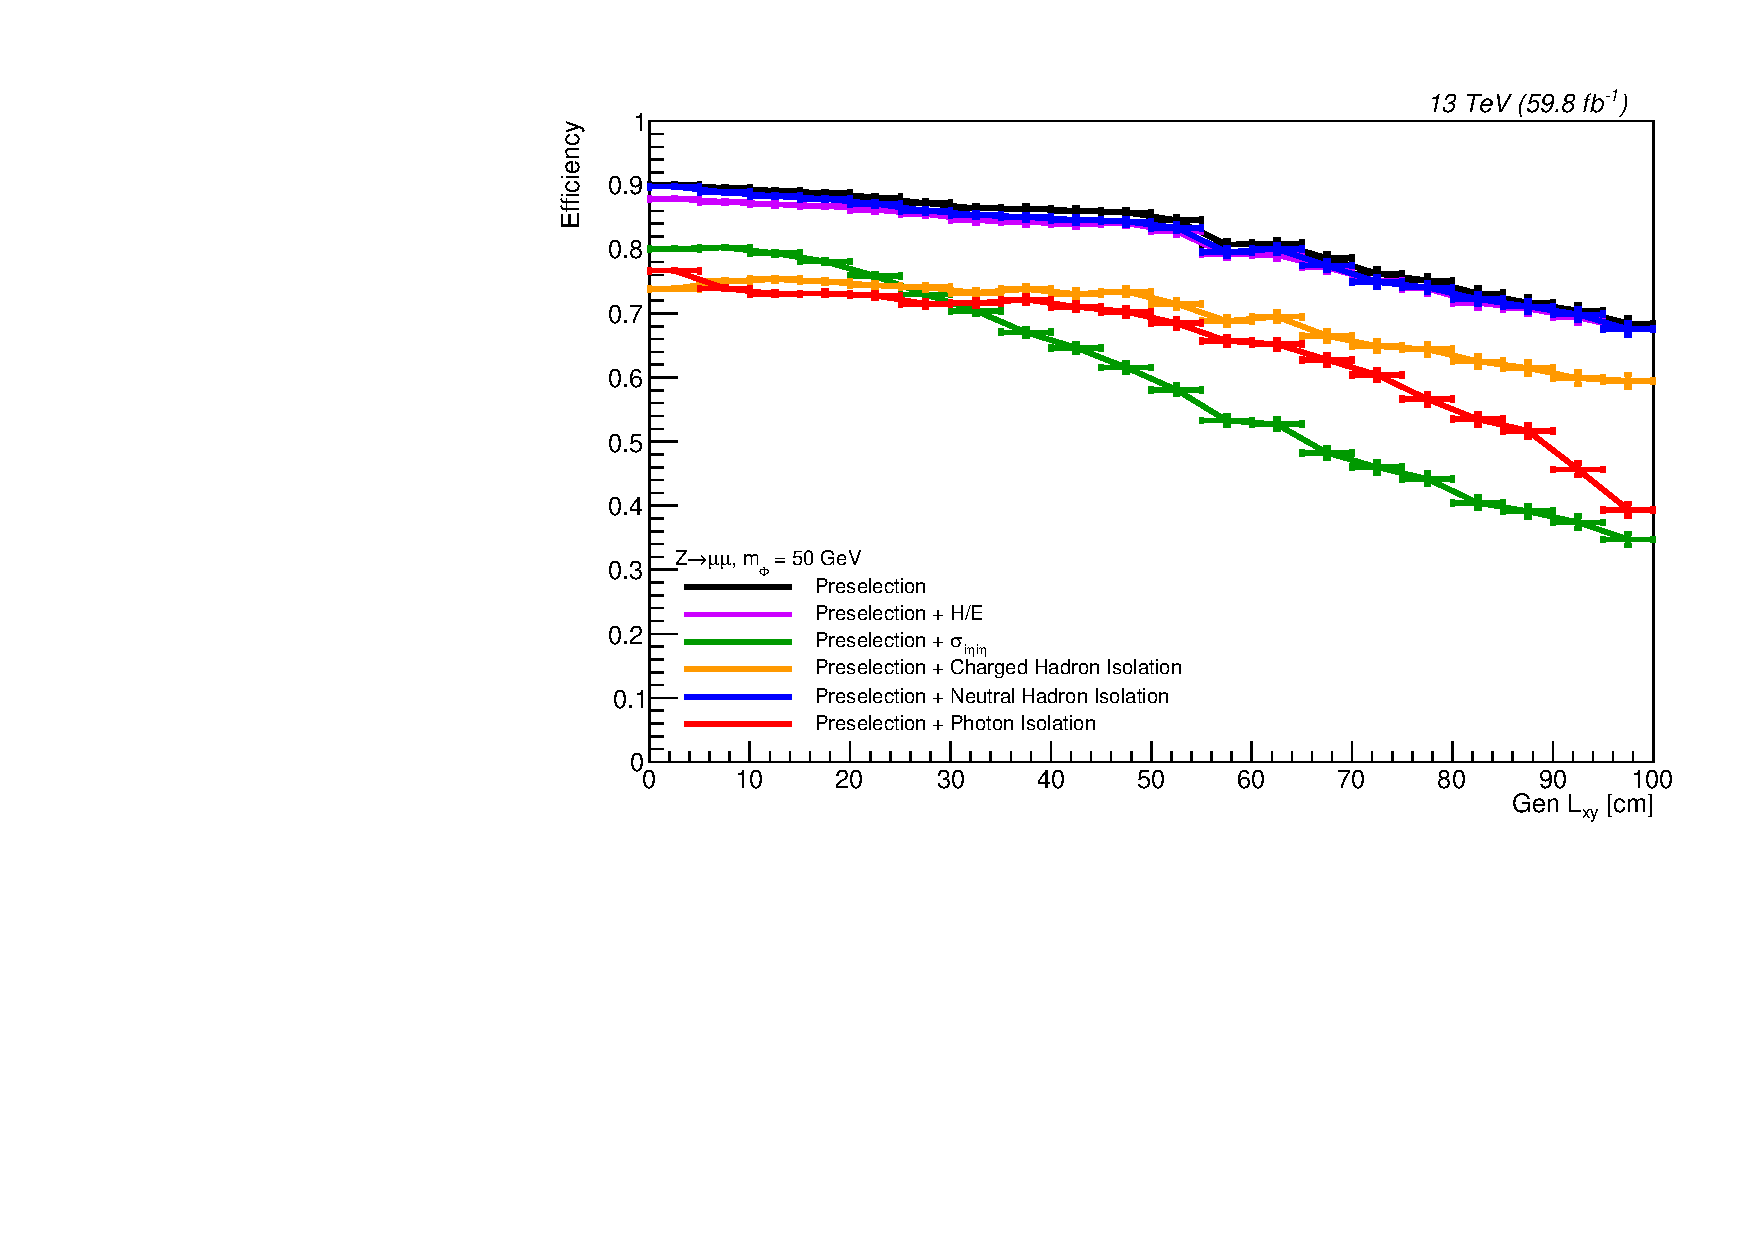
\includegraphics[width=\linewidth]{figs/05_analysis/cutBasedID_effVsLxy_Z_m50_cats_2018.pdf} &
		\includegraphics[width=\linewidth]{figs/05_analysis/cutBasedID_effVsLxy_Z_m55_cats_2018.pdf} \\
	\end{tabular}
	\caption[Efficiency for a photon pair to pass preselection versus generator level \lxy on ZH signal samples for all lifetimes in the $\PZ\to\mu\mu$ category.]{Efficiency for a photon pair to pass preselection versus generator level \lxy on ZH signal samples for all lifetimes in the $\PZ\to\mu\mu$ category. Denominator is all generator level photon pairs with each photon having $\pt>20\GeV$ that decay within the geometric acceptance of the ECAL. The numerator requires two matching ($\Delta r<0.3$, energy within 50\% of gen photon) reconstructed photons passing preselection criteria. Cut based ID is applied on top of preselection, showing that the dominant inefficiencies at high \lxy are due to $I_\gamma$ and $\sigma_{i\eta i\eta}$.}
	\label{fig:Photon_cutBased}
\end{figure}

\subsection{Signal Region Definitions} \label{sec:ana_signalregion}
$\Phi$ candidates are reconstructed from events with at least two photons passing preselection criteria. If there are only two photons that pass preselection, the diphotons are chosen as a possible $\Phi$ candidate. If more than two photons pass this criteria, the photons will be subject to pairing criteria for every candidate mass of the $\Phi$. This pairing process is designed to maximize pairing efficiency, as without pointing capabilities there is no consistent, robust way to determine whether signal photons originated from the same $\Phi$, while also minimizing the bias introduced through the pairing criteria. For each candidate mass, photon pairs are chosen as follows:
\begin{itemize}
	\item The pair with an energetically allowed decay is chosen (i.e. there is a physical solution to equation~\ref{eq:me1e2theta})
	\item If multiple pairs have allowed decays, the pair with more photons passing cut based ID is chosen
	\item If multiple pairs use the same number of photons passing ID, the pair with the largest prompt invariant mass \mgg is chosen
	\item If multiple pairs have the same \mgg, the pair with the highest \ptgg is chosen
\end{itemize}
For convention, the leading higher \pt photon is referred to as $\gamma_1$ while the sub-leading lower \pt photon is referred to as $\gamma_2$.

The signal region is defined by the presence of one \PZ candidate and at least one $\Phi$ candidate composed of two ID'd photons. Events are categorized based on the lepton flavor of the Z decay to either muons or electrons. For each signal region category, an anti-ID control region is utilized for background estimation. These categories are defined identically to the signal region but require the $\Phi$ candidate to use one photon passing the loose cut based ID and one photon failing loose cut based ID defined in table~\ref{tab:photonID}.

To compare data to simulated background, the dilepton mass \mll is plotted in all categories for the signal region and anti-ID control region in figures~\ref{fig:zmass_preselection_med}$\,$-$\,$\ref{fig:zmass_preselection_tight}. These distributions are made agnostic to the vertex calculation and have no cuts on diphoton \lxy. The results show moderate agreement in the anti-ID control region and limited statistical power for simulated events in the ID signal region. Comparisons show an excess of events below $90\GeV$ due to the presence of final state radiation.

\begin{figure}[htb!]
	\centering
	\begin{tabular}{>{\centering\arraybackslash}m{0.32\linewidth} >{\centering\arraybackslash}m{0.32\linewidth} >{\centering\arraybackslash}m{0.32\linewidth}}
		2018 $\PZ\to\mu\mu$ & 2017 $\PZ\to\mu\mu$ & 2016 $\PZ\to\mu\mu$\\
		\includegraphics[width=\linewidth]{figs/05_analysis/2018_ZX_Z_mass_MU_preselection_med.pdf} &
		\includegraphics[width=\linewidth]{figs/05_analysis/2017_ZX_Z_mass_MU_preselection_med.pdf} &
		\includegraphics[width=\linewidth]{figs/05_analysis/2016_ZX_Z_mass_MU_preselection_med.pdf} \\
		2018 $\PZ\to ee$ & 2017 $\PZ\to ee$ & 2016 $\PZ\to ee$\\
		\includegraphics[width=\linewidth]{figs/05_analysis/2018_ZX_Z_mass_ELE_preselection_med.pdf} &
		\includegraphics[width=\linewidth]{figs/05_analysis/2017_ZX_Z_mass_ELE_preselection_med.pdf} &
		\includegraphics[width=\linewidth]{figs/05_analysis/2016_ZX_Z_mass_ELE_preselection_med.pdf} \\
	\end{tabular}
	\caption[m$\left(\ell^+\ell^-\right)$ data and simulated background after preselection criteria across all years in the anti-ID control region.]{m$\left(\ell^+\ell^-\right)$ data and simulated background after preselection criteria across all years in the anti-ID control region. Top row: $\PZ\to\mu\mu$ category. Bottom row: $\PZ\to ee$ category}
	\label{fig:zmass_preselection_med}
\end{figure}
\begin{figure}[htb!]
	\begin{tabular}{>{\centering\arraybackslash}m{0.32\linewidth} >{\centering\arraybackslash}m{0.32\linewidth} >{\centering\arraybackslash}m{0.32\linewidth}}
		2018 $\PZ\to\mu\mu$ & 2017 $\PZ\to\mu\mu$ & 2016 $\PZ\to\mu\mu$\\		
		\includegraphics[width=\linewidth]{figs/05_analysis/2018_ZX_Z_mass_MU_preselection_tight.pdf} &
		\includegraphics[width=\linewidth]{figs/05_analysis/2017_ZX_Z_mass_MU_preselection_tight.pdf} &
		\includegraphics[width=\linewidth]{figs/05_analysis/2016_ZX_Z_mass_MU_preselection_tight.pdf} \\
		2018 $\PZ\to ee$ & 2017 $\PZ\to ee$ & 2016 $\PZ\to ee$\\		
		\includegraphics[width=\linewidth]{figs/05_analysis/2018_ZX_Z_mass_ELE_preselection_tight.pdf} &
		\includegraphics[width=\linewidth]{figs/05_analysis/2017_ZX_Z_mass_ELE_preselection_tight.pdf} &
		\includegraphics[width=\linewidth]{figs/05_analysis/2016_ZX_Z_mass_ELE_preselection_tight.pdf} \\
	\end{tabular}
	\caption[m$\left(\ell^+\ell^-\right)$ data and simulated background after preselection criteria across all years in the ID signal region.]{m$\left(\ell^+\ell^-\right)$ data and simulated background after preselection criteria across all years in the ID signal region. Top row: $\PZ\to\mu\mu$ category. Bottom row: $\PZ\to ee$ category}
	\label{fig:zmass_preselection_tight}
\end{figure}

\subsubsection{Positive and Negative \lxy Regions} \label{sec:ana_lxyregions}
As discussed in section~\ref{sec:ana_vertex}, it is possible for the vertex calculating to yield a negative value of \lxy, indicating that the $\Phi$ would have decayed from behind the beamline relative to the ECAL clusters. The negative \lxy region is used for background estimation, while the positive \lxy region is used for the final signal extraction. To avoid possible signal contamination in the negative \lxy region, we define the two regions using the prompt invariant diphoton mass \mgg. This provides a robust cut that is not dependent on the vertex calculation.

By construction of the vertex constraint, if two photons have a prompt invariant mass $\mgg$ then the vertex calculated assuming $\mphi=\mgg$ would yield an $\lxy=0$. As a corollary, the prompt invariant mass of a pair of displaced photons decaying from a particle of mass $\mphi$ will always have a prompt invariant mass $\mgg\leq\mphi$. Since the mass of the $\Phi$ is constrained by a maximum of $\mh/2$, the highest prompt invariant mass for potential signal events is $\mgg=\mh/2$. Thus cutting on $\mgg>\mh/2$ gives a set of events that yield a negative \lxy for all hypothetical \mphi that is disjoint from any possible signal events.

The positive \lxy signal region is defined by $\mgg<\mphi+5\GeV$. This allows slightly negative \lxy events into the signal region in order to account for the vertex calculation resolution for low displacement signal events.

\subsubsection{Final State Radiation Rejection} \label{sec:ana_fsr}
One source of background occurs when a lepton in the final state radiates a photon, known as final state radiation (FSR). This results in the band of excess events in \mll seen in figures~\ref{fig:zmass_preselection_med}$\,$-$\,$\ref{fig:zmass_preselection_tight}. FSR events are identified by calculating the invariant mass of the dileptons plus one or both of the photons used to reconstruct the $\Phi$ candidate. If the combined invariant mass is within $75-105\GeV$ and closer to the \PZ boson mass of 91\GeV than the original dilepton mass, the event is flagged as having FSR and removed. FSR events are classified based on which combination of photons yields a mass within the \PZ window, with the closest mass to 91\GeV being chosen if multiple satisfy the criteria. The categories are defined as follows:
\begin{itemize}
	\item Tag 1: $\ell\ell+\gamma_1$
	\item Tag 2: $\ell\ell+\gamma_2$
	\item Tag 3: $\ell\ell+\gamma_1+\gamma_2$
\end{itemize}

Figure~\ref{fig:fsr_distributions} show the comparison of invariant mass distributions for all three tags in the $\PZ\to\mu\mu$ category. Simulated background uses the anti-ID control region due to poor statistical power in the ID signal region. Simulated signal uses an $\mphi=20\GeV$, $c\tau=0\unit{mm}$ signal sample, but the distributions remain stable across all masses and lifetimes. It is shown that the largest background contribution comes from tag 2 followed by tag 1. Tag 3 shows minimal contribution, as the energy loss from double FSR photons usually causes the dilepton invariant mass to fall below 70\GeV. 

\begin{figure}[htb!]
	\centering
	\captionsetup[subfigure]{justification=centering}
	\begin{subfigure}[h]{.32\linewidth}
		\centering
		\includegraphics[width=\linewidth]{figs/05_analysis/2018_ZX_Zg1_mass_MU_preFSR_mx20_comp.pdf}
		\caption{m($\mu\mu\gamma_1$)}
	\end{subfigure}
	\begin{subfigure}[h]{.32\linewidth}
		\centering
		\includegraphics[width=\linewidth]{figs/05_analysis/2018_ZX_Zg2_mass_MU_preFSR_mx20_comp.pdf}
		\caption{m($\mu\mu\gamma_2$)}
	\end{subfigure}
	\begin{subfigure}[h]{.32\linewidth}
		\centering
		\includegraphics[width=\linewidth]{figs/05_analysis/2018_ZX_mass_MU_preFSR_mx20_comp.pdf}
		\caption{m($\mu\mu\gamma_1\gamma_2$)}
	\end{subfigure}
	\begin{subfigure}[h]{.32\linewidth}
		\centering
		\includegraphics[width=\linewidth]{figs/05_analysis/2018_ZX_Zg1_mass_ELE_preFSR_mx20_comp.pdf}
		\caption{m($ee\gamma_1$)}
	\end{subfigure}
	\begin{subfigure}[h]{.32\linewidth}
		\centering
		\includegraphics[width=\linewidth]{figs/05_analysis/2018_ZX_Zg2_mass_ELE_preFSR_mx20_comp.pdf}
		\caption{m($ee\gamma_2$)}
	\end{subfigure}
	\begin{subfigure}[h]{.32\linewidth}
		\centering
		\includegraphics[width=\linewidth]{figs/05_analysis/2018_ZX_mass_ELE_preFSR_mx20_comp.pdf}
		\caption{m($ee\gamma_1\gamma_2$)}
	\end{subfigure}
	\caption[Comparison of invariant mass distributions for FSR rejection using simulated $\mphi=20\GeV$, $c\tau=0\unit{mm}$ signal and background. Background uses normalized anti-ID control region events for improved statistics while signal shows ID signal region events.]{Comparison of invariant mass distributions for FSR rejection using simulated $\mphi=20\GeV$, $c\tau=0\unit{mm}$ signal and background. Background uses normalized anti-ID control region events for improved statistics while signal shows ID signal region events.}
	\label{fig:fsr_distributions}
\end{figure}

In the anti-ID control region, this method rejects 16\% of simulated background in the $\PZ\to \mu\mu$ category and 19\% in the $\PZ\to ee$ category. In the ID signal region, this method rejects 9\% of simulated background in the $\PZ\to\mu\mu$ category and 35\% in the $\PZ\to ee$ category. Across all signal masses and lifetimes this method maintains $>99.5\%$ signal efficiency. The data and simulated background distributions after rejecting FSR events are shown in figures~\ref{fig:zmass_postFSR_med}$\,$-$\,$\ref{fig:zmass_postFSR_tight}.

\begin{figure}[htb!]
	\centering
	\begin{tabular}{>{\centering\arraybackslash}m{0.32\linewidth} >{\centering\arraybackslash}m{0.32\linewidth} >{\centering\arraybackslash}m{0.32\linewidth}}
		2018 $\PZ\to\mu\mu$ & 2017 $\PZ\to\mu\mu$ & 2016 $\PZ\to\mu\mu$\\
		\includegraphics[width=\linewidth]{figs/05_analysis/2018_ZX_Z_mass_MU_postFSR_med.pdf} &
		\includegraphics[width=\linewidth]{figs/05_analysis/2017_ZX_Z_mass_MU_postFSR_med.pdf} &
		\includegraphics[width=\linewidth]{figs/05_analysis/2016_ZX_Z_mass_MU_postFSR_med.pdf} \\
		2018 $\PZ\to ee$ & 2017 $\PZ\to ee$ & 2016 $\PZ\to ee$\\
		\includegraphics[width=\linewidth]{figs/05_analysis/2018_ZX_Z_mass_ELE_postFSR_med.pdf} &
		\includegraphics[width=\linewidth]{figs/05_analysis/2017_ZX_Z_mass_ELE_postFSR_med.pdf} &
		\includegraphics[width=\linewidth]{figs/05_analysis/2016_ZX_Z_mass_ELE_postFSR_med.pdf} \\
	\end{tabular}
	\caption[m$\left(\ell^+\ell^-\right)$ data and simulated background after rejecting FSR events across all years in the anti-ID control region.]{m$\left(\ell^+\ell^-\right)$ data and simulated background after rejecting FSR events across all years in the anti-ID control region. Top row: $\PZ\to\mu\mu$ category. Bottom row: $\PZ\to ee$ category}
	\label{fig:zmass_postFSR_med}
\end{figure}
\begin{figure}[htb!]
	\begin{tabular}{>{\centering\arraybackslash}m{0.32\linewidth} >{\centering\arraybackslash}m{0.32\linewidth} >{\centering\arraybackslash}m{0.32\linewidth}}
		2018 $\PZ\to\mu\mu$ & 2017 $\PZ\to\mu\mu$ & 2016 $\PZ\to\mu\mu$\\		
		\includegraphics[width=\linewidth]{figs/05_analysis/2018_ZX_Z_mass_MU_postFSR_tight.pdf} &
		\includegraphics[width=\linewidth]{figs/05_analysis/2017_ZX_Z_mass_MU_postFSR_tight.pdf} &
		\includegraphics[width=\linewidth]{figs/05_analysis/2016_ZX_Z_mass_MU_postFSR_tight.pdf} \\
		2018 $\PZ\to ee$ & 2017 $\PZ\to ee$ & 2016 $\PZ\to ee$\\		
		\includegraphics[width=\linewidth]{figs/05_analysis/2018_ZX_Z_mass_ELE_postFSR_tight.pdf} &
		\includegraphics[width=\linewidth]{figs/05_analysis/2017_ZX_Z_mass_ELE_postFSR_tight.pdf} &
		\includegraphics[width=\linewidth]{figs/05_analysis/2016_ZX_Z_mass_ELE_postFSR_tight.pdf} \\
	\end{tabular}
	\caption[m$\left(\ell^+\ell^-\right)$ data and simulated background after rejecting FSR events across all years in the ID signal region.]{m$\left(\ell^+\ell^-\right)$ data and simulated background after rejecting FSR events across all years in the ID signal region. Top row: $\PZ\to\mu\mu$ category. Bottom row: $\PZ\to ee$ category}
	\label{fig:zmass_postFSR_tight}
\end{figure}

\subsubsection{Low \pt Photon Background} \label{sec:ana_photonpt}
Equation~\ref{eq:me1e2theta} shows that, for energetically allowed decays, the angle between two photons increases monotonically as the assumed value of \mphi increases. The position of the ECAL clusters is fixed, so the vertex becomes more displaced as the angle increases, leading to low \pt photon background with large \lxy. This makes the photon \pt a useful handle to discriminate signal and background. We compare the \pt spectrum of leading and sub-leading photons in the anti-ID control region and signal region for events having a positive \lxy in order to determine optimal cut values. As one additional requirement, when comparing the leading \pt spectrum we select background events where $\gamma_1$ is ID'd and $\gamma_2$ is anti-ID'd (and vice versa when plotting the subleading photon). Plots comparing signal and background \pt distributions for leading and subleading photons can be seen in figure~\ref{fig:pt_comparison}.

\begin{figure}[htb!]
	\centering
	\captionsetup[subfigure]{justification=centering}
	\begin{subfigure}[h]{0.45\linewidth}
		\centering
		\includegraphics[width=\linewidth]{figs/05_analysis/2018_ZX_g1_pt_mx20_MU_comp.pdf}
		\caption{$p_\mathrm{T}(\gamma_1)$ for $\mphi=20\GeV$.}
	\end{subfigure}
	\begin{subfigure}[h]{0.45\linewidth}
		\centering
		\includegraphics[width=\linewidth]{figs/05_analysis/2018_ZX_g2_pt_mx20_MU_comp.pdf}
		\caption{$p_\mathrm{T}(\gamma_2)$ for $\mphi=20\GeV$.}
	\end{subfigure}
	\begin{subfigure}[h]{0.45\linewidth}
		\centering
		\includegraphics[width=\linewidth]{figs/05_analysis/2018_ZX_g1_pt_mx50_MU_comp.pdf}
		\caption{$p_\mathrm{T}(\gamma_2)$ for $\mphi=50\GeV$.}
	\end{subfigure}
	\begin{subfigure}[h]{0.45\linewidth}
		\centering
		\includegraphics[width=\linewidth]{figs/05_analysis/2018_ZX_g2_pt_mx50_MU_comp.pdf}
		\caption{$p_\mathrm{T}(\gamma_2)$ for $\mphi=50\GeV$.}
	\end{subfigure}
	\caption[Comparison of leading and subleading photon \pt in the anti-ID control region and signal region for the $\PZ\to\mu\mu$ category under the assumptions $\mphi=20\GeV$ (top) and $\mphi=50\GeV$ (bottom).]{Comparison of leading and subleading photon \pt in the anti-ID control region and signal region for the $\PZ\to\mu\mu$ category under the assumptions $\mphi=20\GeV$ (top) and $\mphi=50\GeV$ (bottom).}
	\label{fig:pt_comparison}
\end{figure}

The final cuts were chosen to be $p_\mathrm{T}(\gamma_1)>35\GeV$ and $p_\mathrm{T}(\gamma_2)>25\GeV$. These cuts reject between 70-80\% of background and maintain about 70\% signal efficiency. The exact values for background rejection can be seen in table~\ref{tab:cuts_pt}, while the cut efficiency for signal can be seen in figure~\ref{fig:signal_acceptance}.

\begin{table}[htb!]
	\begin{center}
		\caption[Photon \pt cut efficiency on control region background]{Photon \pt cut efficiency on control region background}
		\label{tab:cuts_pt}
		\begin{tabular}{l|l|l}
			\hline
			m$_{\Phi}$ [GeV] & \PZ $\rightarrow \mu \mu$  & \PZ $\rightarrow$ ee\\
			\hline
			15	&	.24	&	.23 \\	
			\hline
			20	&	.27	&	.33 \\
			\hline
			30	&	.27	&	.26 \\
			\hline
			40	&	.29	&	.28 \\
			\hline
			50	&	.29	&	.28 \\
			\hline
			55	&	.30	&	.30 \\
			\hline
		\end{tabular}
	\end{center}
\end{table}

\subsubsection{Final Selection Requirements} \label{sec:ana_final_selection}
The final \lxy agnostic data and Monte Carlo comparison plots after applying the FSR and tight photon \pt cuts can be seen in figures~\ref{fig:zmass_final_med}$\,$-$\,$\ref{fig:zmass_final_tight}. Signal Monte Carlo distributions from the $\mphi=30\GeV$, $c\tau=0\unit{mm}$ samples are overlaid at arbitrary normalization for shape comparison. In the ID signal region, the Monte Carlo background shows poor agreement with data and consists of very few weighted events with limited statistical power. For this reason we opt for a data driven method for background estimation.

\begin{figure}[htb!]
	\begin{tabular}{>{\centering\arraybackslash}m{0.32\linewidth} >{\centering\arraybackslash}m{0.32\linewidth} >{\centering\arraybackslash}m{0.32\linewidth}}
		2018 & 2017 & 2016\\
		\includegraphics[width=\linewidth]{figs/05_analysis/2018_ZX_Z_mass_MU_final_med.pdf} & 
		\includegraphics[width=\linewidth]{figs/05_analysis/2017_ZX_Z_mass_MU_final_med.pdf} & 
		\includegraphics[width=\linewidth]{figs/05_analysis/2016_ZX_Z_mass_MU_final_med.pdf} \\
		anti-ID $\PZ\to\mu\mu$ & anti-ID $\PZ\to\mu\mu$ & anti-ID $\PZ\to\mu\mu$\\
		\includegraphics[width=\linewidth]{figs/05_analysis/2018_ZX_Z_mass_ELE_final_med.pdf} & 
		\includegraphics[width=\linewidth]{figs/05_analysis/2017_ZX_Z_mass_ELE_final_med.pdf} & 
		\includegraphics[width=\linewidth]{figs/05_analysis/2016_ZX_Z_mass_ELE_final_med.pdf} \\
		anti-ID $\PZ\to\mu\mu$ & anti-ID $\PZ\to\mu\mu$ & anti-ID $\PZ\to\mu\mu$\\
	\end{tabular}
	\caption[Final m$\left(\ell^+\ell^-\right)$ distributions for data and simulated samples in the anti-ID control region. Top row: $\PZ\to\mu\mu$ category. Bottom row: $\PZ\to ee$ category.]{Final m$\left(\ell^+\ell^-\right)$ distributions for data and simulated samples in the anti-ID control region. Top row: $\PZ\to\mu\mu$ category. Bottom row: $\PZ\to ee$ category.}
	\label{fig:zmass_final_med}
\end{figure}

\begin{figure}[htb!]
	\begin{tabular}{>{\centering\arraybackslash}m{0.32\linewidth} >{\centering\arraybackslash}m{0.32\linewidth} >{\centering\arraybackslash}m{0.32\linewidth}}
		2018 & 2017 & 2016\\
		\includegraphics[width=\linewidth]{figs/05_analysis/2018_ZX_Z_mass_MU_final_tight.pdf} & 
		\includegraphics[width=\linewidth]{figs/05_analysis/2017_ZX_Z_mass_MU_final_tight.pdf} & 
		\includegraphics[width=\linewidth]{figs/05_analysis/2016_ZX_Z_mass_MU_final_tight.pdf} \\
		ID $\PZ\to\mu\mu$ & ID $\PZ\to\mu\mu$ & ID $\PZ\to\mu\mu$\\
		\includegraphics[width=\linewidth]{figs/05_analysis/2018_ZX_Z_mass_ELE_final_tight.pdf} & 
		\includegraphics[width=\linewidth]{figs/05_analysis/2017_ZX_Z_mass_ELE_final_tight.pdf} & 
		\includegraphics[width=\linewidth]{figs/05_analysis/2016_ZX_Z_mass_ELE_final_tight.pdf} \\
		ID $\PZ\to\mu\mu$ & ID $\PZ\to\mu\mu$ & ID $\PZ\to\mu\mu$\\
	\end{tabular}
	\caption[Final m$\left(\ell^+\ell^-\right)$ distributions for data and simulated samples in the ID signal region. Top row: $\PZ\to\mu\mu$ category. Bottom row: $\PZ\to ee$ category.]{Final m$\left(\ell^+\ell^-\right)$ distributions for data and simulated samples in the ID signal region. Top row: $\PZ\to\mu\mu$ category. Bottom row: $\PZ\to ee$ category.}
	\label{fig:zmass_final_tight}
\end{figure}

The efficiencies and expected yields for simulated background are shown in table~\ref{tab:cuts_bkg}. For signal samples we plot the acceptances as an efficiency relative to the total number of generated events for all masses and lifetimes, separating two photon events where only one $\Phi$ decays to photons and four final state photon events where both $\Phi$ decay to photons. The HLT and object preselection cuts are applied as described in sections~\ref{sec:ana_triggers} and~\ref{sec:ana_preselection}. The FSR rejection cuts are applied, but due to the high signal efficiency the points overlap with the previous cuts on loose cut based ID. The positive \lxy cuts result in a decrease in efficiency in the four photon categories due to mispaired photons, where one photon from each $\Phi$ is chosen to calculate the vertex. The full set of signal efficiency plots are shown in figure~\ref{fig:signal_acceptance}.

\begin{table}[htb!]
	\begin{center}
		\caption[Cutflow table and expected yields on background Monte Carlo in the ID+ID signal region]{Cutflow table and expected yields on background Monte Carlo in the ID+ID signal region}
		\label{tab:cuts_bkg}
		\begin{tabular}{l|l|l}
			& \multicolumn{2}{l}{Simulated Events}\\
			\hline
			Selection & \PZ $\rightarrow \mu \mu$  & \PZ $\rightarrow$ ee\\
			\hline
			\hline
			Initial (from preselection) & 67.4 & 22.1 \\
			\hline
			Final State Radiation & 64.7 & 13.6\\
			\hline
			$\pt(\gamma_1)>35 \text{GeV}, \pt(\gamma_2)>25 \text{GeV}$ & 28.0 & 5.5 \\
			\hline
			\hline
			Total Background Rejection & 59\% & 75\%\\
			\hline
		\end{tabular}
	\end{center}
\end{table}

\begin{figure}[htb!]
	\centering
	\captionsetup[subfigure]{justification=centering}
	\begin{subfigure}[h]{0.49\linewidth}
		\centering
		\includegraphics[width=\linewidth]{figs/05_analysis/2018_signal_2G2Q_Z_MU_efficiency_raw.pdf}
		\caption{$\PZ\to\mu\mu$ in the 2$\gamma$ category.}
	\end{subfigure}
	\begin{subfigure}[h]{0.49\linewidth}
		\centering
		\includegraphics[width=\linewidth]{figs/05_analysis/2018_signal_2G2Q_Z_ELE_efficiency_raw.pdf}
		\caption{$\PZ\to ee$ in the 2$\gamma$ category.}
	\end{subfigure}
	\begin{subfigure}[h]{0.49\linewidth}
		\centering
		\includegraphics[width=\linewidth]{figs/05_analysis/2018_signal_4G_Z_MU_efficiency_raw.pdf}
		\caption{$\PZ\to\mu\mu$ in the 4$\gamma$ category.}
	\end{subfigure}
	\begin{subfigure}[h]{0.49\linewidth}
		\centering
		\includegraphics[width=\linewidth]{figs/05_analysis/2018_signal_4G_Z_ELE_efficiency_raw.pdf}
		\caption{$\PZ\to ee$ in the 4$\gamma$ category.}
	\end{subfigure}
	\caption[Cutflow efficiency for signal events with exactly 2 photons (top) and 4 photons (bottom).]{Cutflow efficiency for signal events with exactly 2 photons (top) and 4 photons (bottom).}
	\label{fig:signal_acceptance}
\end{figure}


\section{Background Estimation} \label{sec:ana_bkg}
The limited statistics in the simulated background samples demand a data-driven method of background estimation. As the statistical estimator used to extract signal involves the \lxy distribution in the positive \lxy signal region, it is crucial to get an accurate estimate of both the yield and shape of the expected background. This section outlines the expected sources of background and the process used to estimate the background using the anti-ID control region and negative \lxy sidebands. We demonstrate closure tests which are used to derive the systematic uncertainties on the background estimation.

\subsection{Sources of Standard Model Background} \label{sec:ana_bkgsources}
There are two main expected SM background contributions originating from the Drell-Yan process, which correspond to combinations of "fake" photons from electromagnetic fluctuations of neutral pions produced in jets or PU, and "real" photons from initial or final state radiation (ISR/FSR). The FSR photons are strongly reducible using invariant mass cuts outlined in section~\ref{sec:ana_fsr}. From studies using generator level information it was determined that the subleading photons primarily originate from jets. A Feynman diagram showing possible sources of background is shown in figure~\ref{fig:bkg_dyjets}.

\begin{figure}[htb!]
	\centering
	% !TEX = root = ../../thesis.tex
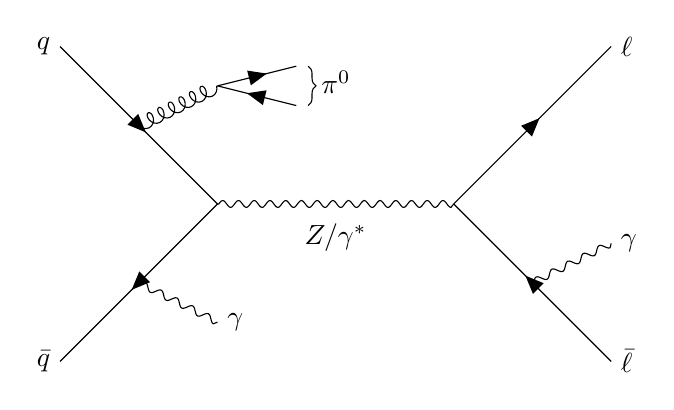
\begin{tikzpicture}
	\begin{feynman}
		% Defining vertex coordinates since \feynmandiagram automatic vertices command needs lualatex to work and I can't figure out how
		\coordinate[label=left:$q$] (i1) at (-3.5, 2); %Initial q
		\coordinate[label=left:$\bar{q}$] (i2) at (-3.5,-2); %Initial qbar
		\coordinate (v1) at (-1.5, 0); %photon vertex 1
		\coordinate (v2) at (1.5, 0);  %photon vertex 2
		\coordinate[label=right:$\ell$] (f1) at (3.5, 2);  %final lepton 1
		\coordinate[label=right:$\bar{\ell}$] (f2) at (3.5, -2); %final lepton 2
		\coordinate (g1) at (-2.5, 1); %gluon vertex 1
		\coordinate (g2) at (-1.5, 1.5); %gluon vertex 2
		\coordinate (q1) at (-.5, 1.75); %pi0 q1
		\coordinate (q2) at (-.5, 1.25); %pi0 q2
		\coordinate (isr1) at (-2.5, -1); %isr v1
		\coordinate[label=right:$\gamma$] (isr2) at (-1.5, -1.5); %isr v2
		\coordinate (fsr1) at (2.5, -1);
		\coordinate[label=right:$\gamma$] (fsr2) at (3.5, -.5);
		
		% Drawing everything
		\draw[fermion] (i1) -- (v1);
		\draw[fermion] (v1) -- (i2);
		\draw[photon] (v1) -- (v2);
		\draw[fermion] (f2) -- (v2);
		\draw[fermion] (v2) -- (f1);
		\draw[gluon] (g1) -- (g2);
		\draw[fermion] (g2) -- (q1);
		\draw[fermion] (q2) -- (g2);
		\draw[photon] (isr1) -- (isr2);
		\draw[photon] (fsr1) -- (fsr2);
		
		% Extra labels
		\draw[black, decorate, decoration={brace, amplitude=.65ex, raise=1ex}] (-.5, 1.75) -- (-.5, 1.25);
		\node[label={right:$\pi^0$}] at (-.43, 1.55){};
		
		\node[label={below:$Z/\gamma^*$}] at (0, 0){};
		
	\end{feynman}
\end{tikzpicture}
	\caption[Feynman diagram showing the possible background contributions from Drell-Yan events. Photons can originate from neutral pions produced in jets, initial state radiation from quarks, or final state radiation from leptons.]{Feynman diagram showing the possible background contributions from Drell-Yan events. Photons can originate from neutral pions produced in jets, initial state radiation from quarks, or final state radiation from leptons.}
	\label{fig:bkg_dyjets}
\end{figure}

There are zero sources of resonant diphoton background expected in this analysis. While the standard model process $\PH\to\gamma\gamma$ produces two final state photons, we expect very few events due to the low branching fraction of 0.0025~\cite{Workman:2022ynf}. For the few events that pass full selection criteria, the invariant diphoton mass of $\mgg=\mh=125\GeV$ would classify events in the negative \lxy sideband by section~\ref{sec:ana_vertex}. This region is used to determine the yield of the expected background and would result in a negligible overestimation of background events.

\subsection{Method of Background Estimation} \label{sec:ana_bkgest}
The largest obstacle towards implementing a reliable background estimation for this analysis was the large statistical fluctuations of the estimated contributions using weights of events in both adjoint regions (e.g. fake-rate based method) and simulation. A mixed-event method which constructs diphotons using leading and sub-leading photons from different events was considered in order to create a large sample of events from uncorrelated combinations of real and fake photons but did not provide an adequate level of closure. In order to account for the correlation between photon kinematics, we predict the shape of the \lxy and \mgg distributions using the anti-ID control region, and normalize the expected number of background events by scaling the anti-ID control region to match the yield of the ID signal region in the negative \lxy sideband. The estimated background in bin $i$ is given by
\begin{equation}
	\label{eq:background}
	N_{\mathrm{bkg}}^{i} = \frac{N(\gamma_\mathrm{ID}+\gamma_\mathrm{ID}, \mgg > \mh/2)}{N(\gamma_\mathrm{ID}+\gamma_\mathrm{antiID}, \mgg > \mh/2)}\times N(\gamma_\mathrm{ID}+\gamma_\mathrm{antiID}, i)
\end{equation}

Where $N(\gamma_\mathrm{ID}+\gamma_\mathrm{(anti)ID}, \mgg > \mh/2)$ is the number of events in the \lxy sideband of the (anti)ID region and $N(\gamma_\mathrm{ID}+\gamma_\mathrm{antiID}, i)$ is the number of events in bin $i$ of the anti-ID control region. 

\subsection{Closure Tests} \label{sec:ana_bkgclosure}
The method of background estimation is validated by comparing the shape of the negative \lxy sidebands in both the ID signal region and anti-ID control region. The behavior of the fit as \lxy approaches zero is used as an indicator for the agreement in the positive \lxy region, and is used to determine the bin-by-bin shape uncertainty. Error bars for the signal and control region data represent the $68\%$ Poisson confidence interval given by
\begin{equation}
	\text{C.I.}=\left[0.5*\chi^2(2N, \alpha/2),\, 0.5*\chi^2(2(N+1), 1-\alpha/2)\right]
\end{equation}
where $\chi^2$ is the chi-square critical value, N is the number of observed events, and $\alpha$ is the significance level of $(1-0.68)$. Since the anti-ID bin contents are scaled in order to match the yield of the ID signal region, the uncertainty is scaled by the same amount.

The anti-ID control region shows compatible values with the ID signal region across all ranges of negative \lxy. Based on the disagreement as \lxy approaches 0, we apply a conservative 40\% uncertainty on each bin in the positive \lxy signal region. The full set of closure plots across all categories for each year can be seen in figures~\ref{fig:bkg_m15}-\ref{fig:bkg_m55}.

\begin{figure}[htb!]
	\centering
	\begin{tabular}{>{\centering\arraybackslash}m{0.45\linewidth} >{\centering\arraybackslash}m{0.45\linewidth}}
		2018 $\PZ\to\mu\mu$ & 2018 $\PZ\to ee$\\
		\includegraphics[width=0.75\linewidth]{figs/05_analysis/closure_ZH_MU_m15_sideband_2018.pdf} &
		\includegraphics[width=0.75\linewidth]{figs/05_analysis/closure_ZH_ELE_m15_sideband_2018.pdf} \\
		2017 $\PZ\to\mu\mu$ & 2017 $\PZ\to ee$\\
		\includegraphics[width=0.75\linewidth]{figs/05_analysis/closure_ZH_MU_m15_sideband_2017.pdf} &
		\includegraphics[width=0.75\linewidth]{figs/05_analysis/closure_ZH_ELE_m15_sideband_2017.pdf} \\
		2016 $\PZ\to\mu\mu$ & 2016 $\PZ\to ee$\\
		\includegraphics[width=0.75\linewidth]{figs/05_analysis/closure_ZH_MU_m15_sideband_2016.pdf} &
		\includegraphics[width=0.75\linewidth]{figs/05_analysis/closure_ZH_ELE_m15_sideband_2016.pdf} \\
	\end{tabular}
	\caption[Shape comparison of ID signal region and anti-ID control region data in the negative \lxy sideband for $\mphi=15\GeV$ in the $\PZ\to\mu\mu$ category (left) and $\PZ\to ee$ category (bottom) across all three years.]{Shape comparison of ID signal region and anti-ID control region data in the negative \lxy sideband for $\mphi=15\GeV$ in the $\PZ\to\mu\mu$ category (left) and $\PZ\to ee$ category (bottom) across all three years.}
	\label{fig:bkg_m15}
\end{figure}

\begin{figure}[htb!]
	\centering
	\begin{tabular}{>{\centering\arraybackslash}m{0.45\linewidth} >{\centering\arraybackslash}m{0.45\linewidth}}
		2018 $\PZ\to\mu\mu$ & 2018 $\PZ\to ee$\\
		\includegraphics[width=0.75\linewidth]{figs/05_analysis/closure_ZH_MU_m20_sideband_2018.pdf} &
		\includegraphics[width=0.75\linewidth]{figs/05_analysis/closure_ZH_ELE_m20_sideband_2018.pdf} \\
		2017 $\PZ\to\mu\mu$ & 2017 $\PZ\to ee$\\
		\includegraphics[width=0.75\linewidth]{figs/05_analysis/closure_ZH_MU_m20_sideband_2017.pdf} &
		\includegraphics[width=0.75\linewidth]{figs/05_analysis/closure_ZH_ELE_m20_sideband_2017.pdf} \\
		2016 $\PZ\to\mu\mu$ & 2016 $\PZ\to ee$\\
		\includegraphics[width=0.75\linewidth]{figs/05_analysis/closure_ZH_MU_m20_sideband_2016.pdf} &
		\includegraphics[width=0.75\linewidth]{figs/05_analysis/closure_ZH_ELE_m20_sideband_2016.pdf} \\
	\end{tabular}
	\caption[Shape comparison of ID signal region and anti-ID control region data in the negative \lxy sideband for $\mphi=20\GeV$ in the $\PZ\to\mu\mu$ category (left) and $\PZ\to ee$ category (bottom) across all three years.]{Shape comparison of ID signal region and anti-ID control region data in the negative \lxy sideband for $\mphi=20\GeV$ in the $\PZ\to\mu\mu$ category (left) and $\PZ\to ee$ category (bottom) across all three years.}
	\label{fig:bkg_m20}
\end{figure}

\begin{figure}[htb!]
	\centering
	\begin{tabular}{>{\centering\arraybackslash}m{0.45\linewidth} >{\centering\arraybackslash}m{0.45\linewidth}}
		2018 $\PZ\to\mu\mu$ & 2018 $\PZ\to ee$\\
		\includegraphics[width=0.75\linewidth]{figs/05_analysis/closure_ZH_MU_m30_sideband_2018.pdf} &
		\includegraphics[width=0.75\linewidth]{figs/05_analysis/closure_ZH_ELE_m30_sideband_2018.pdf} \\
		2017 $\PZ\to\mu\mu$ & 2017 $\PZ\to ee$\\
		\includegraphics[width=0.75\linewidth]{figs/05_analysis/closure_ZH_MU_m30_sideband_2017.pdf} &
		\includegraphics[width=0.75\linewidth]{figs/05_analysis/closure_ZH_ELE_m30_sideband_2017.pdf} \\
		2016 $\PZ\to\mu\mu$ & 2016 $\PZ\to ee$\\
		\includegraphics[width=0.75\linewidth]{figs/05_analysis/closure_ZH_MU_m30_sideband_2016.pdf} &
		\includegraphics[width=0.75\linewidth]{figs/05_analysis/closure_ZH_ELE_m30_sideband_2016.pdf} \\
	\end{tabular}
	\caption[Shape comparison of ID signal region and anti-ID control region data in the negative \lxy sideband for $\mphi=30\GeV$ in the $\PZ\to\mu\mu$ category (left) and $\PZ\to ee$ category (bottom) across all three years.]{Shape comparison of ID signal region and anti-ID control region data in the negative \lxy sideband for $\mphi=30\GeV$ in the $\PZ\to\mu\mu$ category (left) and $\PZ\to ee$ category (bottom) across all three years.}
	\label{fig:bkg_m30}
\end{figure}

\begin{figure}[htb!]
	\centering
	\begin{tabular}{>{\centering\arraybackslash}m{0.45\linewidth} >{\centering\arraybackslash}m{0.45\linewidth}}
		2018 $\PZ\to\mu\mu$ & 2018 $\PZ\to ee$\\
		\includegraphics[width=0.75\linewidth]{figs/05_analysis/closure_ZH_MU_m40_sideband_2018.pdf} &
		\includegraphics[width=0.75\linewidth]{figs/05_analysis/closure_ZH_ELE_m40_sideband_2018.pdf} \\
		2017 $\PZ\to\mu\mu$ & 2017 $\PZ\to ee$\\
		\includegraphics[width=0.75\linewidth]{figs/05_analysis/closure_ZH_MU_m40_sideband_2017.pdf} &
		\includegraphics[width=0.75\linewidth]{figs/05_analysis/closure_ZH_ELE_m40_sideband_2017.pdf} \\
		2016 $\PZ\to\mu\mu$ & 2016 $\PZ\to ee$\\
		\includegraphics[width=0.75\linewidth]{figs/05_analysis/closure_ZH_MU_m40_sideband_2016.pdf} &
		\includegraphics[width=0.75\linewidth]{figs/05_analysis/closure_ZH_ELE_m40_sideband_2016.pdf} \\
	\end{tabular}
	\caption[Shape comparison of ID signal region and anti-ID control region data in the negative \lxy sideband for $\mphi=40\GeV$ in the $\PZ\to\mu\mu$ category (left) and $\PZ\to ee$ category (bottom) across all three years.]{Shape comparison of ID signal region and anti-ID control region data in the negative \lxy sideband for $\mphi=40\GeV$ in the $\PZ\to\mu\mu$ category (left) and $\PZ\to ee$ category (bottom) across all three years.}
	\label{fig:bkg_m40}
\end{figure}

\begin{figure}[htb!]
	\centering
	\begin{tabular}{>{\centering\arraybackslash}m{0.45\linewidth} >{\centering\arraybackslash}m{0.45\linewidth}}
		2018 $\PZ\to\mu\mu$ & 2018 $\PZ\to ee$\\
		\includegraphics[width=0.75\linewidth]{figs/05_analysis/closure_ZH_MU_m50_sideband_2018.pdf} &
		\includegraphics[width=0.75\linewidth]{figs/05_analysis/closure_ZH_ELE_m50_sideband_2018.pdf} \\
		2017 $\PZ\to\mu\mu$ & 2017 $\PZ\to ee$\\
		\includegraphics[width=0.75\linewidth]{figs/05_analysis/closure_ZH_MU_m50_sideband_2017.pdf} &
		\includegraphics[width=0.75\linewidth]{figs/05_analysis/closure_ZH_ELE_m50_sideband_2017.pdf} \\
		2016 $\PZ\to\mu\mu$ & 2016 $\PZ\to ee$\\
		\includegraphics[width=0.75\linewidth]{figs/05_analysis/closure_ZH_MU_m50_sideband_2016.pdf} &
		\includegraphics[width=0.75\linewidth]{figs/05_analysis/closure_ZH_ELE_m50_sideband_2016.pdf} \\
	\end{tabular}
	\caption[Shape comparison of ID signal region and anti-ID control region data in the negative \lxy sideband for $\mphi=50\GeV$ in the $\PZ\to\mu\mu$ category (left) and $\PZ\to ee$ category (bottom) across all three years.]{Shape comparison of ID signal region and anti-ID control region data in the negative \lxy sideband for $\mphi=50\GeV$ in the $\PZ\to\mu\mu$ category (left) and $\PZ\to ee$ category (bottom) across all three years.}
	\label{fig:bkg_m50}
\end{figure}

\begin{figure}[htb!]
	\centering
	\begin{tabular}{>{\centering\arraybackslash}m{0.45\linewidth} >{\centering\arraybackslash}m{0.45\linewidth}}
		2018 $\PZ\to\mu\mu$ & 2018 $\PZ\to ee$\\
		\includegraphics[width=0.75\linewidth]{figs/05_analysis/closure_ZH_MU_m55_sideband_2018.pdf} &
		\includegraphics[width=0.75\linewidth]{figs/05_analysis/closure_ZH_ELE_m55_sideband_2018.pdf} \\
		2017 $\PZ\to\mu\mu$ & 2017 $\PZ\to ee$\\
		\includegraphics[width=0.75\linewidth]{figs/05_analysis/closure_ZH_MU_m55_sideband_2017.pdf} &
		\includegraphics[width=0.75\linewidth]{figs/05_analysis/closure_ZH_ELE_m55_sideband_2017.pdf} \\
		2016 $\PZ\to\mu\mu$ & 2016 $\PZ\to ee$\\
		\includegraphics[width=0.75\linewidth]{figs/05_analysis/closure_ZH_MU_m55_sideband_2016.pdf} &
		\includegraphics[width=0.75\linewidth]{figs/05_analysis/closure_ZH_ELE_m55_sideband_2016.pdf} \\
	\end{tabular}
	\caption[Shape comparison of ID signal region and anti-ID control region data in the negative \lxy sideband for $\mphi=55\GeV$ in the $\PZ\to\mu\mu$ category (left) and $\PZ\to ee$ category (bottom) across all three years.]{Shape comparison of ID signal region and anti-ID control region data in the negative \lxy sideband for $\mphi=55\GeV$ in the $\PZ\to\mu\mu$ category (left) and $\PZ\to ee$ category (bottom) across all three years.}
	\label{fig:bkg_m55}
\end{figure}

\section{Statistical Analysis} \label{sec:ana_stats}
The signal extraction is performed in two dimensional histograms of \lxy and \mgg. The data are binned in four bins of \mgg spanning 4\GeV to $\mphi+5\GeV$ and rows in \lxy spanning from -10\unit{cm} to 100\unit{cm}. Each row represents the \lxy distribution for a given range of \mgg, and is initially binned using a bin width of 1\unit{cm}. Rows are then rebinned using the expected background distribution from anti-ID events derived in section~\ref{sec:ana_bkgest}. For each range of \mgg, the \lxy is rebinned into quantiles of 25\% in order to ensure that there are no bins with zero estimated background. Events in the lowest range of \mgg are binned in quantiles of 50\% due to the limited number of expected background events.

\subsection{Systematic Uncertainties} \label{sec:ana_systs}
Systematic uncertainties are implemented through the use of nuisance parameters which vary the yield of expected signal and background in each bin. For systematic uncertainties that act as multiplicative corrections to the expected yield, the nuisance parameters follow a log-normal (lnN) probability density function (PDF). If the uncertainty for a multiplicative correction is asymmetric, the uncertainty is implemented using asymmetric multiplicative factors scaling with log-normally distributed nuisance parameters. Lastly, the statistical uncertainty from normalization using a control region with $N$ events and a scale factor $\alpha$ is implemented as a systematic uncertainty using a Gamma distribution. The relation between the nuisance parameters and multiplicative corrections for each distribution can be seen in table~\ref{tab:combine_systs}. Systematic uncertainties can be correlated between bins, meaning that the multiplicative corrections for each uncertainty use the same nuisance parameter. Alternatively, uncorrelated uncertainties will each have their own independent nuisance parameter.

\begin{table}[htb!]
	\centering
	\caption[Description of multiplicative corrections for systematic uncertainties as a function of the nuisance parameter $\nu$~\cite{CMS:2024onh}.]{Description of multiplicative corrections for systematic uncertainties as a function of the nuisance parameter $\nu$~\cite{CMS:2024onh}.}
	\label{tab:combine_systs}
	\begin{tabular}{l l c}
		\hline
		Uncertainty Type & Multiplicative Factor $f(\nu)$ & Default Value\\
		\hline
		\hline
		\small\texttt{log-normal}\footnote[1] & $f(\nu)=\kappa^\nu$ & $\nu=0$\\
		\small\texttt{asymmetric log-normal}\footnote[2] & $f(\nu)=\begin{cases}
												\left(\kappa^\text{Down}\right)^{-\nu} & \nu<-0.5\\
												\left(\kappa^\text{Up}\right)^\nu & \nu>0.5\\
												e^{\nu*g(\kappa^\text{Down},\kappa^\text{Up},\nu)} & -0.5<\nu<0.5^*
															\end{cases}$ & $\nu=0$\\
		\small\texttt{Gamma} & $f(\nu)=\nu/N$ & $\nu=N+1$\\
		\hline
		\multicolumn{3}{l}{\footnotesize $^*g(\kappa^\text{Down},\kappa^\text{Up},\nu)=1/8\left[4\ln\left(\kappa^\text{Up}/\kappa^\text{Down}\right)+\ln\left(\kappa^\text{Up}\kappa^\text{Down}\right)(48\nu^5-40\nu^3+15\nu)\right]$}\\
		\multicolumn{3}{l}{\footnote[1] \footnotesize$\kappa=1+\Delta x/x$, where $\Delta x/x$ is the relative uncertainty of multiplicative correction}\\
		\multicolumn{3}{l}{\footnote[2] \footnotesize$\kappa^\text{Up/Down}$ is 1 plus the relative change in $x$ when shifting the uncertainty up/down by 1$\sigma$}\\
	\end{tabular}
\end{table}

These systematic uncertainties show small effects on the expected limits as the analysis is dominated by statistical Poisson uncertainties due to the small number of predicted background events. This section outlines the application of systematic uncertainties on the predicted signal and background. Table~\ref{tab:systs} contains a summary of all systematic uncertainties and the corresponding correlations.

\subsubsection{Signal Uncertainties} \label{sec:ana_systs_sig}
For normalization of signal samples relying on the SM Higgs boson cross section, we apply a theoretical uncertainty of $(-3.1, +3.8)\%$ to the QCD scale and a $\pm1.6\%$ uncertainty in the parton distribution function (PDF) and $\alpha_\mathrm{s}$~\cite{higgsxsec}. These scale factors are applied directly to the normalization of the simulated events. The theoretical uncertainties are 100\% correlated in all categories.

Each scale factor also has a measured uncertainty, which is applied by shifting the nominal weights up or down and reapplying the scale factor. The systematic uncertainty is then taken as the percent change in each bin due to the variation in the scale factors. These are multiplicative uncertainties and applied using asymmetric log-normal constraints. All scale factor uncertainties for the same physics object are 100\% correlated between categories using that object. Therefore photon scale factor uncertainties are correlated between all categories, while the electron/muon uncertainties are only correlated within to the $\PZ\to ee$ and $\PZ\to\mu\mu$ channels respectively. These adjustments generally change the yield on the order of 0.1\%.

Photons in simulated samples have energy corrections to match the mean and uncertainty of their energy resolution to the data. These are applied as a scale correction, which adjusts the central value, and a random smear to match the resolution. Both the scale and smearing corrections have an associated measured uncertainty. Unlike the scale factor corrections described in section~\ref{sec:ana_sf}, which are event level weights, the scale and resolution corrections directly modify the photon energy in each event. In order to adjust the yields based on the scale and resolution uncertainty, the energy of all photons is shifted up or down by the given uncertainty and the relevant distributions for signal extraction are calculated using the shifted values. The residuals when uncertainties are shifted up or down are then taken as the uncertainty. Although this acts as a shape uncertainty, it is implemented as an asymmetric log-normal uncertainty on the yield in each bin. As the corrections are applied to all photons, the nuisance parameters are 100\% correlated between all events.

Luminosity and pileup act as a multiplicative corrections for normalization and are treated as a lnN uncertainty. The corresponding luminosity uncertainties from table~\ref{tab:intLumi} are applied for each year. Since the method used to measure the luminosity is consistent for each year, the luminosity uncertainty is correlated for all categories across all three years of data taking. For the same reason, the 5\% pileup uncertainty is correlated for all years as well.

\subsubsection{Background Uncertainties} \label{sec:ana_systs_bkg}
The predicted background has two systematic uncertainties for the shape and normalization. The shape uncertainty was determined from the non-closure uncertainty from section~\ref{sec:ana_bkgclosure} and is implemented using 40\% lnN in each bin, which is fully uncorrelated between each bin, year, and category. The normalization uncertainty is implemented using a Gamma function and is fully correlated between all bins for the same category and uncorrelated between different categories. This function has two parameters per bin given by $N$ and $\alpha_i$. N symbolizes the number of events in the negative \lxy sideband of the ID signal region and $\alpha_i$ represents the scale factor multiplied by $N$ in order to obtain the expected number of events in bin $i$. Equation~\ref{eq:background} can be rewritten in these terms as
\begin{equation}
	N_\text{bkg}^i=\alpha_i\times N
\end{equation}
where
\begin{equation}
	\alpha_i=\frac{N(\gamma_\mathrm{ID}+\gamma_\mathrm{antiID}, i)}{N(\gamma_\mathrm{ID}+\gamma_\mathrm{antiID}, \mgg > \mh/2)}
\end{equation}
and
\begin{equation}
	N=N(\gamma_\mathrm{ID}+\gamma_\mathrm{ID}, \mgg > \mh/2)
\end{equation}
Under this equivalent interpretation of equation~\ref{eq:background}, the anti-ID control region is used to derive a transfer factor that scales negative \lxy ID region events to positive \lxy signal region events.

\begin{table}[htb!]
	\small
	\caption[Summary of the systematic uncertainties and corresponding correlations]{Summary of the systematic uncertainties and corresponding correlations}  
	\label{tab:systs}
	\centering  
	\begin{tabular}{|c|c|c|c|c|c|} 
		\hline
		Uncertainty    &	Type	& Value(\%)  &  Signal      & Background      &  Correlations\\
		\hline
		QCD scale (ZH) & lnN 	&	$-3.1,+3.8$ & $\surd$     & -               & All categories\\ 
		PDF ($\sigma$) + $\alpha_S$ & lnN	& $\pm 1.6$   & $\surd$     & -               & All categories\\ 
		Photon Energy Scale & lnN & $\pm \sigma$ & $\surd$ & - & All categories\\
		Photon Energy Resolution & lnN & $\pm \sigma$ & $\surd$ & - & All categories\\
		Photon ID 	 & lnN	& $\pm \sigma$ 	& $\surd$ & - & All categories\\
		Photon Pixel Veto & lnN & $\pm \sigma$ 	& $\surd$ & - & All categories\\
		Lepton ID      & lnN 	& $\pm \sigma$   & $\surd$     & -               & Same flavor categories\\ 
		Lepton RECO      & lnN 	& $\pm \sigma$   & $\surd$     & -               & Same flavor categories\\ 
		Muon Isolation      & lnN 	& $\pm \sigma$   & $\surd$     & -               & Muon categories\\ 
		Muon HLT      & lnN 	& $\pm \sigma$   & $\surd$     & -               & Muon categories\\ 
		Electron HLT 	 & lnN	& $\pm \sigma$	  &	$\surd$		& -				  & Electron categories\\
		Luminosity     & lnN	& $1.2-2.5$   & $\surd$     & -               & All categories\\ 
		Pileup	&	lnN	&	$\pm 5.0$ & $\surd$ & - &	All categories \\
		bkg normalization  & gamma & $N\times\alpha$& -  & $\surd$         & Bins in same category\\ 
		bkg non-closure          & lnN & 40 & -  & $\surd$                  & Fully uncorrelated \\ 
		\hline
	\end{tabular}
\end{table}

\subsection{Limit Setting Procedure} \label{sec:ana_limits}
As discussed in section~\ref{sec:ana_mcsig}, the signal samples have been generated using the process $\PH\to\Phi\Phi$ with the $\Phi$ fixed to decay either to a pair of photons or jets with a branching ratio of $50\%$ for each decay channel. The final number of expected signal events is given by
\begin{equation}
	\label{eq:BR}
	N=\lumi\sigma_{\PZ\PH}\varepsilon_\PZ\mathcal{BR}(\PH\to\Phi\Phi)\left ( 2\mathcal{BR} \left ( \Phi \rightarrow \gamma \gamma \right ) \left(1-\mathcal{BR} \left ( \Phi \rightarrow \gamma \gamma \right ) \right ) \varepsilon_{1} +\mathcal{BR} \left ( \Phi \rightarrow \gamma \gamma \right )^2 \varepsilon_{2}  \right )
\end{equation}
where $\varepsilon_\PZ$ is the $\mathcal{BR}(\PZ\to\ell\ell)$ times the efficiency and acceptance to reconstruct leptonic decays of the \PZ, $\varepsilon_{1}$ is the efficiency to reconstruct a photon pair when only one $\Phi$ decays to photons, and $\varepsilon_{2}$ is the efficiency to reconstruct a photon pair when both $\Phi$ decay to photons. Let $\beta=\mathcal{BR}(\Phi\to\gamma\gamma)$. Since we intend to extract the model independent product of the branching fraction of the Higgs boson to two $\Phi$ candidates with the branching fraction of $\Phi\to\gamma\gamma$, we can rewrite equation~\ref{eq:BR} as follows
\begin{equation}
	N=\lumi\sigma_{\PZ\PH}\varepsilon_\PZ\mathcal{BR}(\PH\to\Phi\Phi)\mathcal{BR}(\Phi\to\gamma\gamma)\left (2\varepsilon_{1}(1-\beta)+\varepsilon_{2}\beta  \right )
	\label{eq:BR_beta}
\end{equation}
It is evident that the limit on $\mathcal{BR}(\PH\to\Phi\Phi)\mathcal{BR}(\Phi\to\gamma\gamma)$ will have a model dependence on $\beta$ by a factor of $1/\left[2\varepsilon_{1}(1-\beta)+\varepsilon_{2}\beta\right]$. Isolating the dependence of $\beta$ yields
\begin{equation}
	f(\beta)=\frac{1}{1-(1-\frac{\varepsilon_{2}}{2\varepsilon_{1}})\beta}
	\label{eq:br_dependence}
\end{equation}
This factor ranges from [1, $\frac{2\varepsilon_{1}}{\varepsilon_{2}}$] as $\beta$ goes from 0 to 1. If the reconstruction of each $\Phi$ was independent of the other, then we would expect $\varepsilon_2=1-(1-\varepsilon_1)^2$. In this case, evaluating $f$ for $\beta=1$ would give $f(1)=1/(1-\varepsilon_1/2)>1$. However, it is common to mispair photons from events where only 1 photon from each $\Phi$ passes reconstruction, which inflates $\varepsilon_2$ and leads to $\varepsilon_2>1-(1-\varepsilon_1)^2$, causing $f(1)<1$. This effect is larger for higher values of \mphi as the mispaired $\Phi$ candidate is more likely to pass selection criteria and have a positive \lxy. Results from this analysis are performed using $\beta=0.5$ but can be reinterpreted for other branching ratios by scaling them by equation~\ref{eq:br_dependence}. Figures~\ref{fig:BR_MU} and~\ref{fig:BR_ELE} show the dependence of the limits on $\beta$ for the $\PZ\to\mu\mu$ and $\PZ\to ee$ categories across all hypothetical values of \mphi and $c\tau$.

\begin{figure}[htb!]
	\centering
	\captionsetup[subfigure]{justification=centering}
	\begin{subfigure}{0.3\linewidth}
		\centering
		$\mphi=15\GeV$
		\includegraphics[width=\linewidth]{figs/05_analysis/BR_Z_MU_15.pdf}
	\end{subfigure}
	\begin{subfigure}{0.3\linewidth}
		\centering
		$\mphi=20\GeV$
		\includegraphics[width=\linewidth]{figs/05_analysis/BR_Z_MU_20.pdf}
	\end{subfigure}
	\begin{subfigure}{0.3\linewidth}
		\centering
		$\mphi=30\GeV$
		\includegraphics[width=\linewidth]{figs/05_analysis/BR_Z_MU_30.pdf}
	\end{subfigure}
	\begin{subfigure}{0.3\linewidth}
		\centering
		$\mphi=40\GeV$
		\includegraphics[width=\linewidth]{figs/05_analysis/BR_Z_MU_40.pdf}
	\end{subfigure}
	\begin{subfigure}{0.3\linewidth}
		\centering
		$\mphi=50\GeV$
		\includegraphics[width=\linewidth]{figs/05_analysis/BR_Z_MU_50.pdf}
	\end{subfigure}
	\begin{subfigure}{0.3\linewidth}
		\centering
		$\mphi=55\GeV$
		\includegraphics[width=\linewidth]{figs/05_analysis/BR_Z_MU_55.pdf}
	\end{subfigure}
	\caption[Dependence of the normalization of limits on $\mathcal{BR}(\Phi\to\gamma\gamma)$ for the $\PZ\to\mu\mu$ categories across all masses and values of $c\tau$.]{Dependence of the normalization of limits on $\mathcal{BR}(\Phi\to\gamma\gamma)$ for the $\PZ\to\mu\mu$ categories across all masses and values of $c\tau$.}
	\label{fig:BR_MU}
\end{figure}

\begin{figure}[htb!]
	\centering
	\captionsetup[subfigure]{justification=centering}
	\begin{subfigure}{0.3\linewidth}
		\centering
		$\mphi=15\GeV$
		\includegraphics[width=\linewidth]{figs/05_analysis/BR_Z_ELE_15.pdf}
	\end{subfigure}
	\begin{subfigure}{0.3\linewidth}
		\centering
		$\mphi=20\GeV$
		\includegraphics[width=\linewidth]{figs/05_analysis/BR_Z_ELE_20.pdf}
	\end{subfigure}
	\begin{subfigure}{0.3\linewidth}
		\centering
		$\mphi=30\GeV$
		\includegraphics[width=\linewidth]{figs/05_analysis/BR_Z_ELE_30.pdf}
	\end{subfigure}
	\begin{subfigure}{0.3\linewidth}
		\centering
		$\mphi=40\GeV$
		\includegraphics[width=\linewidth]{figs/05_analysis/BR_Z_ELE_40.pdf}
	\end{subfigure}
	\begin{subfigure}{0.3\linewidth}
		\centering
		$\mphi=50\GeV$
		\includegraphics[width=\linewidth]{figs/05_analysis/BR_Z_ELE_50.pdf}
	\end{subfigure}
	\begin{subfigure}{0.3\linewidth}
		\centering
		$\mphi=55\GeV$
		\includegraphics[width=\linewidth]{figs/05_analysis/BR_Z_ELE_55.pdf}
	\end{subfigure}
	\caption[Dependence of the normalization of limits on $\mathcal{BR}(\Phi\to\gamma\gamma)$ for the $\PZ\to ee$ categories across all masses and values of $c\tau$.]{Dependence of the normalization of limits on $\mathcal{BR}(\Phi\to\gamma\gamma)$ for the $\PZ\to\mu\mu$ categories across all masses and values of $c\tau$.}
	\label{fig:BR_ELE}
\end{figure}

Upper limits are set using the \texttt{combine} toolkit provided by CMS, which was created to combine results from multiple decay channels in the Higgs boson discovery~\cite{CMS:2024onh}. Each bin is treated as a Poisson based likelihood with two contributions: signal and background. For each bin, the number of expected events is given by
\begin{equation}
	\label{eq:expected_events}
	E[n_i]=\mu s_i(\boldsymbol{\theta_s})+b_i(\boldsymbol{\theta_b})
\end{equation}
where $s_i(\boldsymbol{\theta_s})$ and $b_i(\boldsymbol{\theta_b})$ are the expected signal and background events given a set of nuisance parameters $\boldsymbol{\theta}$. Each nuisance parameter is associated with one or more systematic uncertainties outlined in section~\ref{sec:ana_systs}. The total expected background also treated as a nuisance parameter. The variable $\mu$ is the signal strength parameter, with $\mu=0$ corresponding to the background-only, or "null", hypothesis and $\mu=1$ corresponding to the nominal signal hypothesis. In order to extract the signal strength, we allow the nuisance parameters and number of background events to vary in order to define a test statistic $t_\mu$ as
\begin{equation}
	\label{eq:test_stat}
	t_\mu=-2\ln{\frac{\mathcal{L}(\mu, \hat{\boldsymbol{\theta}}(\mu)\,| \, \text{data})}{\mathcal{L(\hat{\mu}, \hat{\boldsymbol{\theta}}(\hat{\mu})\,|\,\text{data})}}}
\end{equation}
The term $\hat{\boldsymbol{\theta}}(\mu)$ represents the set of nuisance parameters that maximizes the likelihood $\mathcal{L}$ for a given value of $\mu$. In the denominator, the term $\hat{\mu}$ represents the signal strength parameter that gives the global maximum of the likelihood. By construction, a lower test statistic indicates higher compatibility between data and a signal strength of $\mu$, while a higher test statistic indicates lower compatibility. For cases where we wish to set an upper limit on a strictly positive signal strength parameter, such as this analysis where a negative signal strength would represent an non-physical solution, the modified test statistic $\tilde{q}_\mu$ is defined as
\begin{equation}
	\label{eq:test_stat2}
	\tilde{q}_\mu=\begin{cases}
		0 & \hat{\mu}>\mu \\
		-2\ln{\frac{\mathcal{L}(\mu,\hat{\boldsymbol{\theta}}(\mu)\,|\,\text{data})}{\mathcal{L(\hat{\mu}, \hat{\boldsymbol{\theta}}(\hat{\mu})\,|\,\text{data})}}} & \mu\geq\hat{\mu}\geq0 \\
		-2\ln{\frac{\mathcal{L}(\mu,\hat{\boldsymbol{\theta}}(\mu)\,|\,\text{data})}{\mathcal{L(\text{0} , \hat{\boldsymbol{\theta}}( \text{0} )\,|\,\text{data})}}} & \hat{\mu}<0
	\end{cases}
\end{equation}

The test statistic follows a probability density function (PDF) denoted as $f(\tilde{q}_\mu|\mu)$, which has an approximate analytic form by applying the Wald approximation~\cite{Cowan_2011}. It is also useful to define the specific test statistic for the case where $\mu=0$ as
\begin{equation}
	\label{eq:test_q0}
	q_0=\begin{cases}
		0 & \hat{\mu}<0\\
		-2\ln{\frac{\mathcal{L}(0, \hat{\boldsymbol{\theta}}(0)\,|\,\text{data})}{\mathcal{L(\hat{\mu}, \hat{\boldsymbol{\theta}}(\hat{\mu})\,|\,\text{data})}}} & \hat{\mu}\geq0
	\end{cases}
\end{equation}
This background only test statistic has its own corresponding PDF denoted by $f(q_0|0)$, once again having an analytic form from the Wald approximation~\cite{Cowan_2011}. It should be noted that while the best fit value $q_{0,\text{obs}}$ is equivalent to the best fit value from $\tilde{q}_\mu$ when $\mu$ is set equal to 0, the PDF is a distinct distribution from $f(\tilde{q}_\mu|\mu)$. From these two PDFs, we define two p-values: the probability of measuring at least this many events given the null hypothesis ($p_b$) and the probability to measure more events given the best fit signal hypothesis ($p_\mu$) as the following: 
\begin{equation}
	\label{eq:pb}
	1-p_b=\int_{q_{0,\text{obs}}}^{\infty}f(q_0|0)dq_0
\end{equation}
\begin{equation}
	\label{eq:p_upper}
	p_\mu=\int_{\tilde{q}_{\mu,\text{obs}}}^{\infty}f(\tilde{q}_\mu|\mu)d\tilde{q}_\mu
\end{equation}
From these two p-values, the modified frequentist confidence limits CL$_\mathrm{s}$ are defined as
\begin{equation}
	\label{eq:cls}
	\text{CL}_\mathrm{s}(\mu)=\frac{p_\mu}{1-p_b}
\end{equation} 
A signal strength of $\mu$ is said to be excluded at a confidence level (CL) of $\alpha$ for CL$_\mathrm{s}(\mu)<1-\alpha$. For example, a value of CL$_\mathrm{s}(\mu)<0.05$ would exclude $\mu$ at 95\% CL.

In order to set a limit on the desired branching ratios, the expected number of signal events described in equation~\ref{eq:BR_beta} are scaled such that $\mu$ represents $\mathcal{BR}(\PH\to\Phi\Phi)\times\mathcal{BR}(\Phi\to\gamma\gamma)$. The simulated signal is normalized using the measured cross section for quark and gluon induced \PZns+\PH production found in table~\ref{tab:higgs_xsec}. The \PZ boson in all signal samples is forced to decay leptonically, so the samples must be normalized to the total leptonic branching ratio to $e, \mu,\text{ and }\tau$ of 0.100986~\cite{Workman:2022ynf}.

\begin{table}[htb!]
	\centering
	\caption[Higgs production cross sections used to normalize simulated signal samples~\cite{higgsxsec}.]{Higgs production cross sections used to normalize simulated signal samples~\cite{higgsxsec}.}
	\label{tab:higgs_xsec}
	\begin{tabular}{l | l}
		\hline
		Production Model & Cross Section\\
		\hline
		\hline
		\ZH & 0.8696\\
		\ggZH & 0.1057\\
		\hline
	\end{tabular}
\end{table}

\subsection{Nuisance Parameter Impacts and Pull Distributions} \label{sec:ana_pulls}
The fitting procedure done by \texttt{combine} has several checks to validate that the nuisance parameter are properly constrained and the fits are well behaved. We provide checks on the pull distributions and impacts of the nuisance parameters. The pull distribution refers to the difference in initial pre-fit and final post-fit values of the nuisance parameters, divided by the initial pre-fit uncertainty. The impact refers to the correlation between a nuisance parameter and the signal strength $\mu$. To calculate the impact of a nuisance parameter, we vary the parameter to its post fit value $\pm1\sigma$ of the post-fit uncertainty, then refit the remaining nuisance parameters and extract the new signal strength. The impact is defined as the difference between the signal strength parameter obtained from this fitting procedure and the signal strength parameter obtained from the nominal fit. Broadly speaking, a larger impact signifies the analysis is more sensitive to a given nuisance parameter. Although performing the fit to data involves calculating the signal strength $\mu$, the exact value is kept unknown in order to remain blinded.

A set of pulls and impacts of the highest impact nuisance parameters for a signal hypothesis of $\mphi=30\GeV$ and c$\tau=100\unit{mm}$ is shown in figure~\ref{fig:impacts}. Central values of the post fit nuisance parameters lie within 1$\sigma$ of the pre-fit values. The post-fit uncertainties are similar to the pre-fit uncertainties, signifying that they are not tightly constrained by the fit process. Impacts are measured for a signal strength parameter corresponding to $\mu=20\times\mathcal{BR}(\PH\to\Phi\Phi)\times\mathcal{BR}(\Phi\to\gamma\gamma)$. The highest impact nuisance parameters shift $\mu$ on the order of $0.5\%$, corresponding to a shift in the product of branching ratios of $0.025\%$.

\begin{figure}[htb!]
	\centering
	\includegraphics[width=\linewidth]{figs/05_analysis/impacts_postFit_m30_ct100.pdf}
	\caption[Post-fit pulls and impacts of the 30 highest impact nuisance parameters for a  $\mphi=30\GeV$, c$\tau=100\unit{mm}$ signal hypothesis. Leftmost column shows the nuisance parameter names. Parameters starting with \texttt{CMS\_bkg}$^*$ represent nuisance parameters for background normalization and non-closure uncertainty; all others correspond to systematic uncertainties of simulated signal. Middle column shows post-fit pull distributions, which lie within 1$\sigma$ of the pre-fit uncertainty. Right column shows the impacts on the signal strength parameter $\mu=20\times\mathcal{BR}(\PH\to\Phi\Phi)\times\mathcal{BR}(\Phi\to\gamma\gamma)$.]{Post-fit pulls and impacts of the 30 highest impact nuisance parameters for a  $\mphi=30\GeV$, c$\tau=100\unit{mm}$ signal hypothesis. Leftmost column shows the nuisance parameter names. Parameters starting with \texttt{CMS\_bkg}$^*$ represent nuisance parameters for background normalization and non-closure uncertainty; all others correspond to systematic uncertainties of simulated signal. Middle column shows post-fit pull distributions, which lie within 1$\sigma$ of the pre-fit uncertainty. Right column shows the impacts on the signal strength parameter $\mu=20\times\mathcal{BR}(\PH\to\Phi\Phi)\times\mathcal{BR}(\Phi\to\gamma\gamma)$.}
	\label{fig:impacts}
\end{figure}

\section{Results} \label{sec:ana_res}
The following section covers the observed data and measured limits for model dependent SM \PZns+\PH production as well as limits on model independent \PZns+$\Phi\Phi$ production.

\subsection{Observed Data} \label{sec:ana_obs}
The observed number of events in the positive \lxy signal region as well as the predicted background are shown for all categories in figures~\ref{fig:results_m15} - \ref{fig:results_m55}. Shaded bands represent the 40\% uncertainty applied to each bin determined by the closure tests. Signal samples with lifetimes $c\tau=0\unit{mm}$ and $100\unit{mm}$ are normalized to $\mathcal{BR}(\PH\to\Phi\Phi)\times\mathcal{BR}(\Phi\to\gamma\gamma)=0.05$ and stacked on the predicted background.

\begin{figure}[htb!]
	\centering
	\begin{tabular}{c c}
		2018 $\PZ\to\mu\mu$ & 2018 $\PZ\to ee$\\
		\includegraphics[width=0.45\linewidth]{figs/05_analysis/closure_ZH_MU_m15_data_2018.pdf} &
		\includegraphics[width=0.45\linewidth]{figs/05_analysis/closure_ZH_ELE_m15_data_2018.pdf} \\
		2017 $\PZ\to\mu\mu$ & 2017 $\PZ\to ee$\\
		\includegraphics[width=0.45\linewidth]{figs/05_analysis/closure_ZH_MU_m15_data_2017.pdf} &
		\includegraphics[width=0.45\linewidth]{figs/05_analysis/closure_ZH_ELE_m15_data_2017.pdf} \\
		2016 $\PZ\to\mu\mu$ & 2016 $\PZ\to ee$\\
		\includegraphics[width=0.45\linewidth]{figs/05_analysis/closure_ZH_MU_m15_data_2016.pdf} &
		\includegraphics[width=0.45\linewidth]{figs/05_analysis/closure_ZH_ELE_m15_data_2016.pdf} \\
	\end{tabular}
	\caption[Observed number of $m_\Phi=15\GeV$ events in the signal region of the $\PZ\to\mu\mu$ category (left) and the $\PZ\to ee$ category (right) across all three years.]{Observed number of $m_\Phi=15\GeV$ events in the signal region of the $\PZ\to\mu\mu$ category (left) and the $\PZ\to ee$ category (right) across all three years.}
	\label{fig:results_m15}
\end{figure}

\begin{figure}[htb!]
	\centering
	\begin{tabular}{c c}
		2018 $\PZ\to\mu\mu$ & 2018 $\PZ\to ee$\\
		\includegraphics[width=0.45\linewidth]{figs/05_analysis/closure_ZH_MU_m20_data_2018.pdf} &
		\includegraphics[width=0.45\linewidth]{figs/05_analysis/closure_ZH_ELE_m20_data_2018.pdf} \\
		2017 $\PZ\to\mu\mu$ & 2017 $\PZ\to ee$\\
		\includegraphics[width=0.45\linewidth]{figs/05_analysis/closure_ZH_MU_m20_data_2017.pdf} &
		\includegraphics[width=0.45\linewidth]{figs/05_analysis/closure_ZH_ELE_m20_data_2017.pdf} \\
		2016 $\PZ\to\mu\mu$ & 2016 $\PZ\to ee$\\
		\includegraphics[width=0.45\linewidth]{figs/05_analysis/closure_ZH_MU_m20_data_2016.pdf} &
		\includegraphics[width=0.45\linewidth]{figs/05_analysis/closure_ZH_ELE_m20_data_2016.pdf} \\
	\end{tabular}
	\caption[Observed number of $m_\Phi=20\GeV$ events in the signal region of the $\PZ\to\mu\mu$ category (left) and the $\PZ\to ee$ category (right) across all three years.]{Observed number of $m_\Phi=20\GeV$ events in the signal region of the $\PZ\to\mu\mu$ category (left) and the $\PZ\to ee$ category (right) across all three years.}
	\label{fig:results_m20}
\end{figure}

\begin{figure}[htb!]
	\centering
	\begin{tabular}{c c}
		2018 $\PZ\to\mu\mu$ & 2018 $\PZ\to ee$\\
		\includegraphics[width=0.45\linewidth]{figs/05_analysis/closure_ZH_MU_m30_data_2018.pdf} &
		\includegraphics[width=0.45\linewidth]{figs/05_analysis/closure_ZH_ELE_m30_data_2018.pdf} \\
		2017 $\PZ\to\mu\mu$ & 2017 $\PZ\to ee$\\
		\includegraphics[width=0.45\linewidth]{figs/05_analysis/closure_ZH_MU_m30_data_2017.pdf} &
		\includegraphics[width=0.45\linewidth]{figs/05_analysis/closure_ZH_ELE_m30_data_2017.pdf} \\
		2016 $\PZ\to\mu\mu$ & 2016 $\PZ\to ee$\\
		\includegraphics[width=0.45\linewidth]{figs/05_analysis/closure_ZH_MU_m30_data_2016.pdf} &
		\includegraphics[width=0.45\linewidth]{figs/05_analysis/closure_ZH_ELE_m30_data_2016.pdf} \\
	\end{tabular}
	\caption[Observed number of $m_\Phi=30\GeV$ events in the signal region of the $\PZ\to\mu\mu$ category (left) and the $\PZ\to ee$ category (right) across all three years.]{Observed number of $m_\Phi=30\GeV$ events in the signal region of the $\PZ\to\mu\mu$ category (left) and the $\PZ\to ee$ category (right) across all three years.}
	\label{fig:results_m30}
\end{figure}

\begin{figure}[htb!]
	\centering
	\begin{tabular}{c c}
		2018 $\PZ\to\mu\mu$ & 2018 $\PZ\to ee$\\
		\includegraphics[width=0.45\linewidth]{figs/05_analysis/closure_ZH_MU_m40_data_2018.pdf} &
		\includegraphics[width=0.45\linewidth]{figs/05_analysis/closure_ZH_ELE_m40_data_2018.pdf} \\
		2017 $\PZ\to\mu\mu$ & 2017 $\PZ\to ee$\\
		\includegraphics[width=0.45\linewidth]{figs/05_analysis/closure_ZH_MU_m40_data_2017.pdf} &
		\includegraphics[width=0.45\linewidth]{figs/05_analysis/closure_ZH_ELE_m40_data_2017.pdf} \\
		2016 $\PZ\to\mu\mu$ & 2016 $\PZ\to ee$\\
		\includegraphics[width=0.45\linewidth]{figs/05_analysis/closure_ZH_MU_m40_data_2016.pdf} &
		\includegraphics[width=0.45\linewidth]{figs/05_analysis/closure_ZH_ELE_m40_data_2016.pdf} \\
	\end{tabular}
	\caption[Observed number of $m_\Phi=40\GeV$ events in the signal region of the $\PZ\to\mu\mu$ category (left) and the $\PZ\to ee$ category (right) across all three years.]{Observed number of $m_\Phi=40\GeV$ events in the signal region of the $\PZ\to\mu\mu$ category (left) and the $\PZ\to ee$ category (right) across all three years.}
	\label{fig:results_m40}
\end{figure}

\begin{figure}[htb!]
	\centering
	\begin{tabular}{c c}
		2018 $\PZ\to\mu\mu$ & 2018 $\PZ\to ee$\\
		\includegraphics[width=0.45\linewidth]{figs/05_analysis/closure_ZH_MU_m50_data_2018.pdf} &
		\includegraphics[width=0.45\linewidth]{figs/05_analysis/closure_ZH_ELE_m50_data_2018.pdf} \\
		2017 $\PZ\to\mu\mu$ & 2017 $\PZ\to ee$\\
		\includegraphics[width=0.45\linewidth]{figs/05_analysis/closure_ZH_MU_m50_data_2017.pdf} &
		\includegraphics[width=0.45\linewidth]{figs/05_analysis/closure_ZH_ELE_m50_data_2017.pdf} \\
		2016 $\PZ\to\mu\mu$ & 2016 $\PZ\to ee$\\
		\includegraphics[width=0.45\linewidth]{figs/05_analysis/closure_ZH_MU_m50_data_2016.pdf} &
		\includegraphics[width=0.45\linewidth]{figs/05_analysis/closure_ZH_ELE_m50_data_2016.pdf} \\
	\end{tabular}
	\caption[Observed number of $m_\Phi=50\GeV$ events in the signal region of the $\PZ\to\mu\mu$ category (left) and the $\PZ\to ee$ category (right) across all three years.]{Observed number of $m_\Phi=50\GeV$ events in the signal region of the $\PZ\to\mu\mu$ category (left) and the $\PZ\to ee$ category (right) across all three years.}
	\label{fig:results_m50}
\end{figure}

\begin{figure}[htb!]
	\centering
	\begin{tabular}{c c}
		2018 $\PZ\to\mu\mu$ & 2018 $\PZ\to ee$\\
		\includegraphics[width=0.45\linewidth]{figs/05_analysis/closure_ZH_MU_m55_data_2018.pdf} &
		\includegraphics[width=0.45\linewidth]{figs/05_analysis/closure_ZH_ELE_m55_data_2018.pdf} \\
		2017 $\PZ\to\mu\mu$ & 2017 $\PZ\to ee$\\
		\includegraphics[width=0.45\linewidth]{figs/05_analysis/closure_ZH_MU_m55_data_2017.pdf} &
		\includegraphics[width=0.45\linewidth]{figs/05_analysis/closure_ZH_ELE_m55_data_2017.pdf} \\
		2016 $\PZ\to\mu\mu$ & 2016 $\PZ\to ee$\\
		\includegraphics[width=0.45\linewidth]{figs/05_analysis/closure_ZH_MU_m55_data_2016.pdf} &
		\includegraphics[width=0.45\linewidth]{figs/05_analysis/closure_ZH_ELE_m55_data_2016.pdf} \\
	\end{tabular}
	\caption[Observed number of $m_\Phi=55\GeV$ events in the signal region of the $\PZ\to\mu\mu$ category (left) and the $\PZ\to ee$ category (right) across all three years.]{Observed number of $m_\Phi=55\GeV$ events in the signal region of the $\PZ\to\mu\mu$ category (left) and the $\PZ\to ee$ category (right) across all three years.}
	\label{fig:results_m55}
\end{figure}

\subsection{Model Dependent Upper Limits} \label{sec:ana_moddepUL}
The expected and observed limits are interpreted using the asymptotic CL$_\mathrm{s}$ method described in section~\ref{sec:ana_limits}. Upper 95\% CL limits are set on a signal strength parameter corresponding to $\mathcal{BR}(\PH\to\Phi\Phi)\times\mathcal{BR}(\Phi\to\gamma\gamma)$ assuming the associated production of a \PZ boson and SM Higgs boson. Results are presented as a function of $\mathrm{c}\tau$ for all candidate signal masses listed in section~\ref{sec:ana_mcsig}. Limits are interpolated between the centrally provided and reweighted lifetimes. The one-dimensional limits versus c$\tau$ for all candidate mass points are shown in figure~\ref{fig:limits_MD_1D}. Two-dimensional limit plots of \mphi versus c$\tau$ shown in figure~\ref{fig:limits_MD_2D} also interpolate between the $\mphi$ points given from centrally produced signal samples.

\begin{figure}[htb!]
	\centering
	\begin{tabular}{c c c}
		\includegraphics[width=0.31\linewidth]{figs/05_analysis/limitVsCtau_ZH_m15_Run2.pdf} &
		\includegraphics[width=0.31\linewidth]{figs/05_analysis/limitVsCtau_ZH_m20_Run2.pdf} &
		\includegraphics[width=0.31\linewidth]{figs/05_analysis/limitVsCtau_ZH_m30_Run2.pdf}\\
		\includegraphics[width=0.31\linewidth]{figs/05_analysis/limitVsCtau_ZH_m40_Run2.pdf}&
		\includegraphics[width=0.31\linewidth]{figs/05_analysis/limitVsCtau_ZH_m50_Run2.pdf}&
		\includegraphics[width=0.31\linewidth]{figs/05_analysis/limitVsCtau_ZH_m55_Run2.pdf}\\
	\end{tabular}
	\caption[Model dependent upper limits for $\mathcal{BR} (\PH \to \Phi\Phi)\times\mathcal{BR} (\Phi \to \gamma\gamma)$ for different values of $m_\Phi$ and $c\tau$ under the assumption that $\mathcal{BR} (\Phi \to \gamma\gamma) =0.5$.]{Model dependent upper limits for $\mathcal{BR} (\PH \to \Phi\Phi)\times\mathcal{BR} (\Phi \to \gamma\gamma)$ for different values of $m_\Phi$ and $c\tau$ under the assumption that $\mathcal{BR} (\Phi \to \gamma\gamma) =0.5$.}
	\label{fig:limits_MD_1D}
\end{figure}

The peak sensitivity occurs at intermediate mass points around $\mphi=30\GeV$ and low to intermediate lifetimes below $50\unit{mm}$. As mass increases, the diphoton $I_\gamma$ cut efficiency increases because the $\Delta R$ between the two photons increases with \mphi, while the $\sigma_{i\eta i\eta}$ efficiency decreases as the shower shape becomes more skewed. Additionally, the estimated background also increases, as there are more diphoton events that can reconstruct a vertex in the positive \lxy signal region. These two effects cause peak sensitivity at intermediate values of \mphi. The behavior of the limits versus c$\tau$ at low lifetimes is dominated by the intrinsic resolution of the vertex fit. Since the signal distributions vary negligibly below c$\tau=3\unit{mm}$, the limits also remain constant. Due to this, the range of lifetimes is only shown to a minimum of 0.1\unit{mm} but show a constant value below this. At intermediate lifetimes around $10\unit{mm}$ the signal distributions become distinct, but do not produce significant improvements to the upper limits. This is because the background distribution \lxy is not determined from the tracker information or from detector pointing capabilities but from calculations based on the energy and separation of the photons. Because of this, the expected background does not steeply fall with \lxy.

\begin{figure}[htb!]
	\centering
	\includegraphics[width=0.75\linewidth]{figs/05_analysis/obs_2D_mVsCtau_ZH_Run2.pdf}
	\caption[Observed limit of $\mathcal{BR} (\PH \to \Phi\Phi)\times\mathcal{BR} (\Phi \to \gamma\gamma)$ as a function of $m_\Phi$ and $c\tau$ under the assumption that $\mathcal{BR} (\Phi \to \gamma\gamma) =0.5$.] {Observed limit of $\mathcal{BR} (\PH \to \Phi\Phi)\times\mathcal{BR} (\Phi \to \gamma\gamma)$ as a function of $m_\Phi$ and $c\tau$ under the assumption that $\mathcal{BR} (\Phi \to \gamma\gamma) =0.5$.}
	\label{fig:limits_MD_2D}
\end{figure}

\subsection{Model Independent Upper Limits} \label{sec:ana_modelindepUL}
The previous model dependent limits assume that a SM Higgs boson was created and decayed directly to $\Phi\Phi$ by normalizing the expected events using the SM cross section $\sigma(\PZ\PH)$. However, some models such as those discussed in chapter~\ref{chap:theory} predict the existence of BSM Higgs bosons, which would have different couplings than the SM Higgs. We present reinterpreted upper limits on a signal strength parameter $\mu=\sigma(\PZns+\Phi\Phi)\times\mathcal{BR}(\Phi\to\gamma\gamma)$ by normalizing the number of expected signal events to a cross section to $\sigma(\PZns+\Phi\Phi)=1\unit{pb}$.

\begin{figure}[htb!]
	\centering
	\begin{tabular}{c c c}
	\includegraphics[width=0.31\linewidth]{figs/05_analysis/limitVsCtau_ZH_m15_Run2_modelIndependent.pdf} &
	\includegraphics[width=0.31\linewidth]{figs/05_analysis/limitVsCtau_ZH_m20_Run2_modelIndependent.pdf} &
	\includegraphics[width=0.31\linewidth]{figs/05_analysis/limitVsCtau_ZH_m30_Run2_modelIndependent.pdf} \\
	\includegraphics[width=0.31\linewidth]{figs/05_analysis/limitVsCtau_ZH_m40_Run2_modelIndependent.pdf} &
	\includegraphics[width=0.31\linewidth]{figs/05_analysis/limitVsCtau_ZH_m50_Run2_modelIndependent.pdf} &
	\includegraphics[width=0.31\linewidth]{figs/05_analysis/limitVsCtau_ZH_m55_Run2_modelIndependent.pdf}\\
	\end{tabular}
	\caption[Model independent upper limits for $\sigma(\PZns+\Phi\Phi)\times\mathcal{BR}(\Phi\to\gamma\gamma)$ as a function of c$\tau$ for various values of \mphi under the assumption that $\mathcal{BR} (\Phi \to \gamma\gamma) =0.5$.]{Model independent upper limits for $\sigma(\PZns+\Phi\Phi)\times\mathcal{BR}(\Phi\to\gamma\gamma)$ as a function of c$\tau$ for various values of \mphi under the assumption that $\mathcal{BR} (\Phi \to \gamma\gamma) =0.5$.}
	\label{fig:limits_MIndep_1D}
\end{figure}

\begin{figure}[htb!]
	\centering
	\includegraphics[width=0.75\linewidth]{figs/05_analysis/obs_2D_ZH_mVsCtau_Run2_modelIndependent.pdf}
	\caption[Observed model independent limits on $\sigma(\PZns+\Phi\Phi)\times\mathcal{BR}(\Phi\to\gamma\gamma)$ as a function of \mphi and c$\tau$ under the assumption that $\mathcal{BR} (\Phi \to \gamma\gamma) =0.5$.]{Observed model independent limits on $\sigma(\PZns+\Phi\Phi)\times\mathcal{BR}(\Phi\to\gamma\gamma)$ as a function of \mphi and c$\tau$ under the assumption that $\mathcal{BR} (\Phi \to \gamma\gamma) =0.5$.}
	\label{fig:limits_MIndep_2D}
\end{figure}

\section{Summary} \label{sec:ana_conclusion}
This analysis presents a search for rare Higgs boson decays to two long-lived scalar bosons decaying to two photons. We use data collected from 2016 to 2018 from center of mass energy $\sqrt{s}=13\unit{TeV}$ proton-proton collisions corresponding to 138\unit{fb^{-1}}. A novel vertex reconstruction technique described in section~\ref{sec:ana_vertex} is used to calculate the vertex of displaced photon pairs using kinematic constraints with a resolution of $<3\unit{cm}$. The reconstructed vertices are used to extract upper limits on the signal strength using a maximum likelihood approach outlined in section~\ref{sec:ana_stats}. We set limits on the product of the SM Higgs boson branching ratio to long-lived scalar bosons $\Phi$ times the branching ratio of the $\Phi$ boson to two photons for a wide range of hypothetical $\Phi$ masses and lifetimes. No significant excesses are observed in the data and upper limits are calculated for the product of branching ratios below $1\%$.

Results from this analysis validate the diphoton vertex reconstruction as a viable method to set limits on long lived photon decays. At the time of writing this dissertation, there is work in progress to extend this analysis for additional Higgs boson production mechanisms. Higgs boson production with an associated \PW boson is a natural extension that can follow the event selection and signal extraction procedure outlined above. In parallel, an analysis searching for Higgs production through gluon fusion will extract the signal strength using the invariant mass of the four photons to reconstruct the Higgs boson mass. The four photon mass resolution shows improvements by correcting the photon four-momentum using the vertex constraint, which is expected to improve the expected limits. Preliminary plans to use Higgs bosons produced through vector boson fusion are ongoing. These analyses are expected to show improved results by incorporating data taken from 2022 to 2024, which currently corresponds to a recorded $91.49\unit{fb^{-1}}$~\cite{CMSlumi}.
\begin{appendices}
	% !TEX = root../thesis.tex
\chapter{Mathematical Formalism of the Standard Model} \label{sec:sm_theory}

\section{Quantum Field Theory and Lagrangian Mechanics} \label{sec:sm_theory_qft}
In classical mechanics, the Lagrangian of a system is defined as $L=T-U$, where $T$ is the kinetic energy and $U$ is the potential energy. The Lagrangian is a function of coordinates $q_i$ and their time derivatives $\dot{q}_i$, and is used to derive the equations of motion using the Euler-Lagrange equations
\begin{equation}
	\label{eq:eulerlagrange_cm}
	\dv{}{t}\left(\pdv{L}{\dot{q}_i}\right)-\pdv{L}{q_i}=0
\end{equation}
This method fails, however, to describe systems where both quantum mechanical and relativistic effects are significant. In this regime, we rely on quantum field theory (QFT), which replaces the Lagrangian with a Lagrangian density
\begin{equation}
	L(q_i,\dot{q}_i)\to\mathcal{L}(\phi_i,\partial_\mu\phi_i)\\
\end{equation}
and the coordinates $q_i(t)$ with fields $\phi_i(x,y,z,t)$, which are functions of both position and time~\cite{Thomson_2013}. For conciseness, we will refer to the Lagrangian density as the Lagrangian in the context of QFT. The Euler-Lagrange equations then become
\begin{equation}
	\label{eq:eulerlagrange_qft}
	\partial_\mu\left(\pdv{\mathcal{L}}{(\partial_\mu\phi_i)}\right)-\pdv{\mathcal{L}}{\phi_i}=0
\end{equation}
For the Standard Model, we require the equations of motion for the scalar field (spin-0), spinor field (spin-1/2), and vector field (spin-1). The corresponding free (i.e. non-interacting) Lagrangians for these fields are given by
\begin{equation}\label{eq:lagrangians}
	\mathcal{L}_0=\frac{1}{2}\left(\partial_\mu\phi\right)\left(\partial^\mu\phi\right)-\frac{1}{2}m^2\phi^2\quad \ 
	\mathcal{L}_{1/2}=i\bar{\psi}\gamma^\mu\partial_\mu\psi-m\bar{\psi}\psi \quad \ 
	\mathcal{L}_{1}=-\frac{1}{16\pi}F^{\mu\nu}F_{\mu\nu}+\frac{1}{8\pi}m^2A^\mu A_\mu
\end{equation}
where $\phi$ is a scalar field, $\psi$ is a spinor field, $\bar{\psi}$ is the adjoint spinor defined by $\bar{\psi}\equiv\psi^\dagger\gamma^0$, $A^\mu$ is a vector field, and $F^{\mu\nu}\equiv\partial^\mu A^\nu-\partial^\nu A^\mu$. The derivative terms in the free Lagrangians can be thought of as analogs to the kinetic energy terms in the classical Lagrangian, while the masses are given by the coefficients to the quadratic terms. Beginning with $\mathcal{L}_0$, the derivatives in equation~\ref{eq:eulerlagrange_qft} give the following equation of motion:
\begin{gather}
	\pdv{\mathcal{L}}{\phi}=-m^2\phi \qquad
	\pdv{\mathcal{L}}{(\partial_0\phi)}=\partial_0\phi=\partial^0\phi \qquad
	\pdv{\mathcal{L}}{(\partial_k\phi)}=-\partial_k\phi=\partial^k\phi	\\
	\Rightarrow \partial_\mu\partial^\mu\phi+m^2\phi=0 \label{eq:kg_eqn}
\end{gather}
Here, we follow the standard convention $k=1,2,3$ which sums over the spatial indices of the spacetime coordinates. Equation~\ref{eq:kg_eqn} is known as the Klein-Gordon equation. For $\mathcal{L}_{1/2}$, we treat $\psi$ and $\bar{\psi}$ as two independent field variables. Repeating the process for the spin-1/2 Lagrangian yields
\begin{gather}
	\pdv{\mathcal{L}}{(\partial_\mu\psi)}=-m\bar{\psi} \qquad \pdv{\mathcal{L}}{\psi}=i\bar{\psi}\gamma^\mu \qquad
	\pdv{\mathcal{L}}{(\partial_\mu\bar{\psi})}=0 \qquad
	\pdv{\mathcal{L}}{\bar{\psi}}=i\gamma^\mu\partial_\mu\psi-m\psi	\\
	\Rightarrow i\partial_\mu\bar{\psi}\gamma^\mu+m\bar{\psi}=0 \quad \text{and} \quad i\gamma^\mu\partial_\mu\psi-m\psi=0 \label{eq:dirac_eqn}
\end{gather}
The two expressions in equation~\ref{eq:dirac_eqn} are equivalent and are referred to as the Dirac Equation. Lastly, solving $\mathcal{L}_1$ gives the following
\begin{gather}
	\pdv{\mathcal{L}}{(\partial_\mu A_\nu)}=-\frac{1}{4\pi}F^{\mu\nu} \qquad \pdv{\mathcal{L}}{A_\nu}=\frac{1}{4\pi}m^2A^\nu \\
	\Rightarrow \partial_\mu F^{\mu\nu}-m^2A^\nu=0 \label{eq:proca_eqn}
\end{gather}
Equation~\ref{eq:proca_eqn} is known as the Proca equation. It is no coincidence that this equation with m=0 resembles the covariant form of Maxwell's equation with no sources with $A^\mu=(\phi, \mathbf{A})$, where $\phi$ is the electric (scalar) potential and $\mathbf{A}$ is the magnetic (vector) potential. Recall that the photon is the massless, spin-1 mediator of the electromagnetic force, and this equation was derived from the free Lagrangian for a spin-1 field. This connection will be explored in greater detail in the section~\ref{sec:sm_theory_gauge}.

\section{Gauge Theory and Local Gauge Invariance} \label{sec:sm_theory_gauge}
A Lagrangian is said to be gauge invariant under a symmetry transformation $\hat{U}$ that takes $\phi\to\phi'=\hat{U}\phi$ if $\mathcal{L}\to\mathcal{L}'=\mathcal{L}$. The basis for the standard model relies on taking invariance under a \textit{global} symmetry $\hat{U}$ and requiring invariance under the \textit{local} symmetry $\hat{U}(x)$ (here $x$ is written as shorthand for $x^\mu$, the spacetime coordinates). This promotion from global to local symmetry introduces new vector fields to the free Lagrangian, which are forced to transform in specific ways due to the required gauge invariance. These new vector fields represent the gauge bosons and introduce the interaction terms to the free Lagrangians in equation~\ref{eq:lagrangians}.

For a concrete example, we take the spin-1/2 Dirac Lagrangian and transform it under $\hat{U}=e^{iq\theta}$. The fields transform as
\begin{equation}
	\psi\to\psi'=e^{iq\theta}\psi \qquad \bar{\psi}\to\bar{\psi}'= \bar{\psi}e^{-iq\theta} =e^{-iq\theta}\bar{\psi}
\end{equation}
It is trivial to show that $\mathcal{L}\to\mathcal{L}'=\mathcal{L}$, as $\psi\bar{\psi}\to\psi'\bar{\psi}'=e^{iq\theta}e^{-iq\theta}\psi\bar{\psi}=\psi\bar{\psi}$. However, when we promote the global symmetry to a local symmetry, the transformation becomes $\hat{U}(x)=e^{i\theta(x)}$ and the Lagrangian transforms as
\begin{align}
	\mathcal{L}\to\mathcal{L}'&=ie^{-iq\theta(x)}\bar{\psi}\gamma^\mu\partial_\mu(e^{iq\theta(x)}\psi)-me^{-iq\theta(x)}\bar{\psi}e^{iq\theta(x)}\psi\\
	&=ie^{-iq\theta(x)}\bar{\psi}\gamma^\mu\left(iq(\partial_\mu\theta(x))e^{iq\theta(x)}\psi+e^{iq\theta(x)}\partial_\mu\psi\right)-m\bar{\psi}\psi\\
	&=\mathcal{L}-q(\partial_\mu\theta(x))\bar{\psi}\gamma^\mu\psi
\end{align}
The spin-1/2 Lagrangian, evidently, will require an extra term to remain locally gauge invariant. The form of this term can be derived from the \textit{minimal coupling rule}~\cite{griffiths_gauge}. By defining a covariant derivative $\partial_\mu\to D_\mu\equiv\partial_\mu+iqA_\mu$, where the new vector field $A_\mu$ transforms as $A_\mu\to A_\mu'\equiv A_\mu+\partial_\mu\lambda$, we transform the Lagrangian to determine $\lambda$ which satisfies the gauge invariance. The new Lagrangian becomes \begin{equation}
	\mathcal{L}=i\bar{\psi}\gamma^\mu\left(\partial_\mu+iqA_\mu\right)\psi-m\bar{\psi}\psi
\end{equation}
and transforms as
\begin{align}
	\mathcal{L}\to\mathcal{L}'&=i\bar{\psi}e^{-iq\theta(x)}\gamma^\mu\left(\partial_\mu+iq(A_\mu+\partial_\mu\lambda)\right)(e^{iq\theta(x)}\psi)-m\bar{\psi}e^{-iq\theta(x)}e^{iq\theta(x)}\psi\\
	&=\mathcal{L}-q\bar{\psi}\gamma^\mu\psi\left(\partial_\mu\theta(x)-\partial_\mu\lambda\right)
\end{align}
Therefore we can determine that $\lambda=\theta(x)$ and the new vector field must transform as $A_\mu\to A_\mu'=A_\mu+\partial_\mu\theta(x)$. In order to complete the Lagrangian and account for this new vector field, we must add the terms from the Proca Lagrangian. The new Lagrangian then becomes
\begin{equation}
	\mathcal{L}=i\bar{\psi}\gamma^\mu\partial_\mu\psi-q\bar{\psi}\gamma^\mu A_\mu\psi-m\bar{\psi}\psi-\frac{1}{16\pi}F^{\mu\nu}F_{\mu\nu}+\frac{1}{4\pi}m_{A}^2A^\mu A_\mu
\end{equation}
This Lagrangian must again be checked to see if it remains locally gauge invariant. The first three terms have been shown to be locally gauge invariant by construction. The fourth term remains invariant, as the partial derivatives on $\theta(x)$ commute, giving $\partial_\mu\partial_\nu\theta-\partial_\nu\partial_\mu\theta=0$. The last term transforms as
\begin{align}
	A^\mu A_\mu\to A^{\prime\mu}A_\mu^\prime&=(A^\mu+\partial^\mu\theta(x))(A_\mu+\partial_\mu\theta(x))\\
	&=A^\mu A_\mu+A^\mu\partial_\mu\theta(x)+A_\mu\partial^\mu\theta(x)+\partial^\mu\partial_\mu\theta(x)\neq A^\mu A_\mu
\end{align}
Because $A^\mu A_\mu$ is not locally gauge invariant, it follows that the mass $m_{A}$ must equal 0. The full Lagrangian is then
\begin{equation}
	\mathcal{L}_\text{QED}=i\bar{\psi}\gamma^\mu\partial_\mu\psi-m\bar{\psi}\psi-\frac{1}{16\pi}F^{\mu\nu}F_{\mu\nu}-q\bar{\psi}\gamma^\mu\psi A_\mu
\end{equation}
This is known as the quantum electrodynamic (QED) Lagrangian, which models the electromagnetic force. The relation of $\mathcal{L}_\text{QED}$ to Maxwell's equations can be seen by applying the Euler-Lagrange equations on the field $A^\mu$, which gives
\begin{equation}
	\label{eq:maxwell}
	\partial_\mu F^{\mu\nu}=4\pi j^\nu
\end{equation}
where we have identified the four-vector current as $j^\nu=q\bar{\psi}\gamma^\nu\psi$. Thus the covariant form of Maxwell's equations can be derived from the spin-1/2 Lagrangian by requiring local symmetry under the transformation $\hat{U}(x)=e^{iq\theta(x)}$. From this, the photon can be seen to be the massless gauge boson of the $A^\mu$ vector field, and the electron/positron can be identified with the spinors $\psi$ and $\bar{\psi}$.

The transformation $\hat{U}=e^{iq\theta}$ satisfies the requirement $\hat{U}^\dagger\hat{U}=1$, which defines the unitary group U(1). Thus, we say that the QED Lagrangian is derived by requiring local U(1) gauge symmetry. In a similar manner, the Lagrangian for the unified electroweak force and strong force can be derived using an $SU(2)\otimes U(1)$ and $SU(3)$ gauge symmetry respectively, though the process is substantially more complicated as the transformation is non-abelian. In general, the global gauge symmetry is under the transformation $\hat{U}=e^{iqg_\mu a^\mu}$, where $g_\mu$ are the generators of the group, $a^\mu$ are the parameters corresponding to each generator, and $q$ represents the coupling strength. For $U(1)$, which represents rotations around the unit circle, the generator is 1 and the parameter $\theta$ is the  the rotation angle. Table~\ref{tab:generators} shows the generators for $U(1)$, $SU(2)$, and $SU(3)$.

\begin{table}[htb!]
	\centering
	\caption[List of generators for the unitary group $U(1)$ and special unitary groups $SU(2)$ and $SU(3)$. The 3 generators of $SU(2)$ are the Pauli matrices, while the 8 generators of $SU(3)$ are the Gell-Mann matrices.]{List of generators for the unitary group $U(1)$ and special unitary groups $SU(2)$ and $SU(3)$. The 3 generators of $SU(2)$ are the Pauli matrices, while the 8 generators of $SU(3)$ are the Gell-Mann matrices.}
	\label{tab:generators}
	\begin{tabular}{l | c}
		Group & Generators\\
		\hline
		\hline
		U(1) & 1\\
		\hline & \\[-1.75ex]
		SU(2) & $\tau_1=\frac{1}{2}\sigma_1=\frac{1}{2}\begin{pmatrix}0&1\\1&0\end{pmatrix}$, $\tau_2=\frac{1}{2}\sigma_2=\frac{1}{2}\begin{pmatrix}0&-i\\i&0\end{pmatrix}$, $\tau_3=\frac{1}{2}\sigma_3=\frac{1}{2}\begin{pmatrix}1&0\\0&-1\end{pmatrix}$\\[10pt]
		\hline & \\[-1.75ex]
		SU(3) & \begin{tabular}{l}$\lambda_1=\begin{pmatrix}0&1&0\\1&0&0\\0&0&0\end{pmatrix}$, $\lambda_2=\begin{pmatrix}0&-i&0\\i&0&0\\0&0&0\end{pmatrix}$, $\lambda_3=\begin{pmatrix}1&0&0\\0&-1&0\\0&0&0\end{pmatrix}$\\[20pt]
			$\lambda_4=\begin{pmatrix}0&0&1\\0&0&0\\1&0&0\end{pmatrix}$, $\lambda_5=\begin{pmatrix}0&0&-i\\0&0&0\\i&0&0\end{pmatrix}$\\[20pt]
			$\lambda_6=\begin{pmatrix}0&0&0\\0&0&1\\0&1&0\end{pmatrix}$, 
			$\lambda_7=\begin{pmatrix}0&0&0\\0&0&-i\\0&i&0\end{pmatrix}$, 
			$\lambda_8=\frac{1}{3}\begin{pmatrix}1&0&0\\0&1&0\\0&0&-2\end{pmatrix}$\end{tabular}
	\end{tabular}
\end{table}

As a whole, the standard model is said to be invariant under the symmetry group
\begin{equation}
	\label{eq:sm_gauge}
	SU(3)_C \otimes SU(2)_L \otimes U(1)_Y
\end{equation}
where $\otimes$ is the direct product of the symmetry groups. $SU(3)_C$ represents the symmetry leading to the strong force and conservation of color $C$. The combination of $SU(2)_L\otimes U(1)_Y$ describes the unified electroweak force, which consolidates the weak and electromagnetic force into one symmetry group. The $SU(2)_L$ group represents weak coupling to left-handed chiral particles (or right-handed chiral antiparticles) and leads to the conservation of weak isospin $I^3$. The $U(1)_Y$ group, different from the $U(1)_\text{EM}$ derived previously, represents couplings to both left and right-handed particles and leads to the conservation of weak hypercharge $Y$.

\subsection{The Strong Force} \label{sec:sm_theory_strong}
From equation~\ref{eq:sm_gauge}, the gauge symmetry $SU(3)_C$ is used to describe the strong force. The three quark flavors give three separate fields $\psi_i$, which we notate in the following derivation as
\begin{equation}
	\psi=\begin{pmatrix}\psi_r\\ \psi_b \\ \psi_g\end{pmatrix} \qquad \bar{\psi}=\begin{pmatrix}\bar{\psi}_r & \bar{\psi}_b & \bar{\psi}_g\end{pmatrix}
\end{equation}
Using table~\ref{tab:generators}, we can identify the local transformation as $\hat{U}(x)=e^{-ig_s\boldsymbol{\lambda}\cdot\boldsymbol{\phi}(x)}$, where $\lambda_i\in\{\lambda_1,...,\lambda_8\}$. Defining the covariant derivative as
\begin{equation}
	D_\mu\equiv\partial_\mu+ig_s\boldsymbol{\lambda}\cdot \mathbf{A}_\mu
\end{equation}
the usual method transforming the spin-1/2 Lagrangian to determine how $\mathbf{A}_\mu$ transforms gives
\begin{equation}
	\boldsymbol{\lambda}\cdot\mathbf{A}^\prime_\mu=e^{-ig_s\boldsymbol{\lambda}\cdot\boldsymbol{\phi}(x)}\left(\boldsymbol{\lambda}\cdot\mathbf{A}_\mu\right)+\frac{i}{g}\partial_\mu\left(e^{-ig_s\boldsymbol{\lambda}\cdot\boldsymbol{\phi}(x)}\right)e^{ig_s\boldsymbol{\lambda}\cdot\boldsymbol{\phi}(x)}
\end{equation}
and introduces the interaction term $-g_s\bar{\psi}\gamma^\mu\boldsymbol{\lambda}\psi\cdot\mathbf{A}_\mu$. It follows that we must add the Proca Lagrangian to introduce the kinetic terms for the gauge fields $\mathbf{A}_\mu$. The first term $F^{\mu\nu}F_{\mu\nu}$ must be adjusted to accommodate for the fact that $\mathbf{A}_\mu$ is a \textit{vector} of 8 vector fields, which follows from the 8 generators of $SU(3)$. It can be shown that a generalized definition of the gauge invariant $F^{\mu\nu}$ using the covariant derivative is $F^{\mu\nu}=-\frac{i}{g}[D_\mu,D_\nu]$~\cite{flournoy}. From this, we can derive the invariant form of $F_{\mu\nu}$ as
\begin{equation}
	\label{eq:qcd_fmunu}
	F_{\mu\nu}^a=\partial_\mu A^a_\nu-\partial_\nu A^a_\mu-2gf^{abc}A^b_\mu A^c_\nu
\end{equation}
where we have used the property $[\lambda_i,\lambda_j]=2if^{ijk}\lambda_k$ and $a\in\{1,...,8\}$ represents each element of $\mathbf{F}_{\mu\nu}$. The constants $f^{abc}$ are the anti-symmetric structure constants of $SU(3)$. The mass term is not invariant under the gauge transformation, meaning that $m=0$. We can recognize the 8 massless gauge bosons as the 8 octet configurations of the gluon, which can self-interact due to the terms in equation~\ref{eq:qcd_fmunu}. The final Lagrangian for the strong interaction is then
\begin{equation}
	\mathcal{L}_\text{QCD}=\left[i\bar{\psi}\gamma^\mu\partial_\mu\psi-m\bar{\psi}\psi\right]-q\bar{\psi}\gamma^\mu\lambda^a\psi A_\mu^a-\frac{1}{16\pi}F^{a\mu\nu}F^{a}_{\mu\nu}
\end{equation}
where $a$ is an implicit sum over $\{1,...,8\}$.

\subsection{The Electroweak Force} \label{sec:sm_theory_ew}
The $SU(2)_L\otimes U(1)_Y$ symmetry group describes the unified weak and electromagnetic forces. Because the $SU(2)_L$ group only acts on the left-handed chiral particles, the spinors in the Dirac equation must be projected into left and right-handed chiral states $\psi_R=\frac{1}{2}(1-\gamma^5)\psi$ and $\psi_L=\frac{1}{2}(1+\gamma^5)\psi$. The Dirac Lagrangian then becomes
\begin{equation}
	\mathcal{L}=i\bar{\psi}_L\gamma^\mu\partial_\mu\psi_L+i\bar{\psi}_R\gamma^\mu\partial_\mu\psi_R+m\left(\bar{\psi}_L\psi_R+\bar{\psi}_R\psi_L\right)
\end{equation}
The left-handed fermion doublets, which are coupled with $SU(2)_L$, take the form of
\begin{equation}
	\label{eq:lh_doublets}
	\chi_L=\begin{pmatrix}\PGne\\ \Pe\end{pmatrix}_L, \begin{pmatrix}\PGnGm\\ \PGm\end{pmatrix}_L, \begin{pmatrix}\PGnGt\\ \PGt\end{pmatrix}_L, \begin{pmatrix}\PQu\\ \PQdpr\end{pmatrix}_L, \begin{pmatrix}\PQc\\ \PQspr\end{pmatrix}_L,\begin{pmatrix}\PQt\\ \PQbpr\end{pmatrix}_L
\end{equation}
where $\PQq'$ are quarks that have been rotated into their CKM weak flavor eigenstates. The right handed singlets are more simply represented by $\chi_R=\Pell_R,\PQq_R$ where $\Pell$ is any charged lepton and $\PQq_R$ is any quark, which have isospin $I^3=0$. Neutrinos, notably, are omitted from the right handed singlets because only left-handed neutrinos have been experimentally observed. The transformations from $SU(2)_L$ and $U(1)_Y$ are given by
\begin{align}
	\label{eq:ew_spinor_transform}
	SU(2)_L:& \qquad \chi_L\to\chi_L'=e^{-ig\boldsymbol{\tau}\cdot\boldsymbol{\theta}(x)}\chi_L\\
	U(1)_Y:& \qquad \chi_L\to\chi_L'=e^{ig'\frac{1}{2}Y_L\phi(x)}\chi_L \qquad \chi_R\to \chi_R'=e^{ig'\frac{1}{2}Y_R\phi(x)}\chi_R
\end{align}
The covariant derivatives must act differently on the doublet and singlet states. For the doublets, it must introduce three new gauge fields for $SU(2)$ and one gauge field for $U(1)$. For the singlet, the covariant derivative only introduces the gauge field for the $U(1)$ symmetry. $Y_L$ and $Y_R$ are additional parameters which allow different fractions of charge $g'$ to be carried by left and right handed fermions. By convention, the gauge fields for $SU(2)$ are labeled as $\mathbf{W}_\mu$ while the gauge field for $U(1)$ is labeled as $B_\mu$. Following the previous examples, the covariant derivatives will act on the fields as
\begin{align}
	\label{eq:ew_cov_derivative}
	\partial_\mu\chi_L\to&D_\mu\chi_L\equiv\frac{1}{2}\left(2\partial_\mu\chi_L+ig\boldsymbol{\sigma}\cdot\mathbf{W}_\mu\chi_L+ig'Y_{L}B_\mu\chi_L\right)\\
	\partial_\mu\chi_R\to&D_\mu\chi_R\equiv\frac{1}{2}\left(2\partial_\mu\chi_R+ig'Y_{R}B_\mu\chi_R\right)
\end{align}
From the covariant derivatives, the interaction terms between the vector fields and the fermion fields are given by
\begin{equation}
	\label{eq:ew_interaction}
	\mathcal{L}_\text{int}=-g\bar{\chi}_L\gamma^\mu\boldsymbol{\sigma}\cdot\mathbf{W}_\mu\chi_L-g'\bar{\chi}_L\gamma^\mu Y_{L}B_\mu\chi_L-g'\bar{\chi_R}\gamma^\mu Y_{R} B_\mu\chi_R
\end{equation}
The interaction associated with the $B_\mu$ field connects same handed fermions to their anti-particles. The $B_\mu$ field transforms as expected as $B_\mu\to B_\mu'=B_\mu+\partial_\mu\phi$ since the symmetry group is the same as the derivation of the QED Lagrangian. The $\mathbf{W}_\mu$ fields transform as
\begin{equation}
	\boldsymbol{\sigma}\cdot\mathbf{W}_\mu\to\boldsymbol{\sigma}\cdot\mathbf{W}_\mu'=e^{-ig\boldsymbol{\sigma}\cdot\boldsymbol{\theta}(x)}\boldsymbol{\sigma}\cdot\mathbf{W}_\mu e^{ig\boldsymbol{\sigma}\cdot\boldsymbol{\theta}(x)}+\frac{i}{g}\partial_\mu\left(e^{-ig\boldsymbol{\sigma}\cdot\boldsymbol{\theta}(x)}\right)e^{ig\boldsymbol{\sigma}\cdot\boldsymbol{\theta}(x)}
\end{equation}
The kinetic term for $B_\mu$ takes the usual form of $F^{\mu\nu}=\partial^\mu B^\nu-\partial^\nu B^\mu$. For $\mathbf{W}_\mu$, using the gauge invariant definition of $F^{a}_{\mu\nu}=\frac{-i}{g}[D_\mu,D_\nu]^a$ we get
\begin{equation}
	F^{a}_{\mu\nu}=\partial_\mu W_\nu^a-\partial_\nu W_\mu^a-g\epsilon^{abc}W_\mu^bW_\nu^c
\end{equation}
where $\epsilon^{abc}$ is the anti-symmetric Levi-Civita symbol. The last term indicates that, as with $SU(3)$, the non-abelian gauge results in vector fields that can interact with one another.

In equation~\ref{eq:maxwell}, we identified the QED current $j^\nu$ using the interaction term. Analogously, the weak currents can be inferred from equation~\ref{eq:ew_interaction} as
\begin{equation}
	j_i^\mu=g\bar{\chi}_L\gamma^\mu\sigma_i\chi_L
\end{equation}
The weak currents have natural expressions in terms of the ladder operators $j_\pm^\mu=\frac{1}{\sqrt{2}}(j_1^\mu\pm ij_2^\mu)$, which are analogous to the raising/lowering operators used for angular momentum due to the common group symmetry of $SU(2)$. The weak gauge fields can then be expressed in terms of $W^\pm_\mu=\frac{1}{\sqrt{2}}(W^1_\mu\mp iW_\mu^2)$ to get
\begin{equation}
	\mathbf{j}^\mu\cdot\mathbf{W}_\mu=j_+^\mu W_\mu^++j_-^\mu W_\mu^-+j_3^\mu W_\mu^3
\end{equation}
Without loss of generality, the weak currents explicitly written in terms of the first generation lepton doublet $\chi_L=\begin{pmatrix}\PGne\\\Pe\end{pmatrix}_L$ are
\begin{align}
	j_+^\mu&=\frac{g}{\sqrt{2}}\PAGne_L\gamma^\mu\Pe_L=\frac{g}{\sqrt{2}}\PAGne\gamma^\mu\frac{1}{2}(1-\gamma^5)\Pe\\
	j_-^\mu&=\frac{g}{\sqrt{2}}\PAe_L\gamma^\mu\PAGne_L=\frac{g}{\sqrt{2}}\PAe\gamma^\mu\frac{1}{2}(1-\gamma^5)\PGne\\
	j_3^\mu&=g\left(\PAGne_L\gamma^\mu\PGne_L-\PAe_L\gamma^\mu\Pe_L\right)=\frac{g}{2}\left(\PAGne\gamma^\mu(1-\gamma^5)\PGne-\PAe\gamma^\mu(1-\gamma^5)\Pe\right)
\end{align}
The charged currents $j_\pm^\mu$ can be seen to connect fermions in the left-handed doublets, thus the associated vector fields $W^\pm$ correspond to the \PWpm boson. Naively, the neutral $SU(2)$ field $W_\mu^3$ and neutral $U(1)$ field $B_\mu$ would appear to be associated with the \PZ boson and photon respectively. Instead, due to spontaneous symmetry breaking that will be discussed in section~\ref{sec:sm_theory_higgs}, the \PZ boson and photon are given by a linear combination of $W_\mu^3$ and $B_\mu$ as
\begin{equation}
	\label{eq:ew_mixing}
	\begin{pmatrix}A_\mu\\Z_\mu\end{pmatrix}=\begin{pmatrix}\cos\theta_w&\sin\theta_w\\-\sin\theta_w&\cos\theta_w\end{pmatrix} \begin{pmatrix}B_\mu\\W_\mu^3\end{pmatrix}
\end{equation}
The parameter $\theta_w$ is known as the Weinberg angle, and is determined by coupling strength of the $B_\mu$ and $W_\mu^3$ fields as
\begin{equation}
	\cos\theta_w=\frac{g}{\sqrt{g^2+g'^2}} \qquad \sin\theta_w=\frac{g'}{\sqrt{g^2+g'^2}}
\end{equation}
The coupling strength for the neutral gauge bosons are then given by
\begin{equation}
	g_\gamma=g\sin\theta_w=g'\cos\theta_w \qquad g_Z=\frac{g}{\cos\theta_w}=\frac{g'}{\sin\theta_w}
\end{equation}

The relation between the electroweak currents and the electromagnetic currents can be seen through the conserved charges of the $SU(2)_L\otimes U(1)_Y$ gauge symmetry. Drawing inspiration from the strong interactions, Glashow hypothesized that the weak analog of the Gell-Mann--Nishijima formula would take the form $Q=I^3+\frac{1}{2}Y$, where the electric charge $Q$ is related to the third component of weak isospin $I^3$ and weak hypercharge $Y$~\cite{weakisospin}. Isospin comes from the relation of $SU(2)$ and $\sigma_3$ to angular momentum, while hypercharge is analogous to quark strangeness. Table~\ref{tab:ew_numbers} shows the value of these numbers for right and left-handed quarks and leptons.

\begingroup
\renewcommand*{\arraystretch}{1.25}
\begin{table}[htb!]
	\centering
	\caption[Electroweak quantum numbers for the first generation of fermions, separated for right and left-handed states. Higher generation fermions have identical values.]{Electroweak quantum numbers for the first generation of fermions, separated for right and left-handed states. Higher generation fermions have identical values.}
	\label{tab:ew_numbers}
	\begin{tabular}{l c c c |l c c c}
		\multicolumn{4}{c|}{Left-Handed Doublets} & \multicolumn{4}{c}{Right-Handed Singlets}\\
		\hline
		\hline
		Fermion & $Q_\text{EM}$ & $I^3$ & $Y$ & Fermion & $Q_\text{EM}$ & $I^3$ & $Y$\\
		\hline
		& & & & & & &\\[-1.75ex]
		$\begin{pmatrix}\PGne\\\Pe\end{pmatrix}_L$ & $\begin{pmatrix}0\\-1\end{pmatrix}$ & $\begin{pmatrix}+\frac{1}{2}\\-\frac{1}{2}\end{pmatrix}$ & $\begin{pmatrix}-1\\-1\end{pmatrix}$ & $\Pe_R$ & -1 & 0 & -2\\[20pt]
		\multirow{2}{*}{$\begin{pmatrix}\PQu\\\PQdpr\end{pmatrix}_L$} & \multirow{2}{*}{$\begin{pmatrix}+\frac{2}{3}\\-\frac{1}{3}\end{pmatrix}$} & \multirow{2}{*}{$\begin{pmatrix}+\frac{1}{2}\\-\frac{1}{2}\end{pmatrix}$} & \multirow{2}{*}{$\begin{pmatrix}+\frac{1}{3}\\-\frac{1}{3}\end{pmatrix}$} & $\PQu_R$ & $+\frac{2}{3}$ & 0 & $+\frac{4}{3}$\\
		& & & & $\PQd_R$ & $-\frac{1}{3}$ & 0 & $-\frac{2}{3}$
	\end{tabular}
\end{table}
\endgroup

\section{The Higgs Boson} \label{sec:sm_theory_higgs}
There exist two substantial problems with the derivation of the unified electroweak gauge theory in section~\ref{sec:sm_theory_ew}. Firstly, the mass term in the Proca Lagrangian for the $\mathbf{W}_\mu$ gauge fields is not invariant under $SU(2)$ symmetry transformations. Secondly, the mass term for the spinor field $\psi$ contains both left and right-handed spinors, which transform differently according to equation~\ref{eq:ew_spinor_transform}, meaning this term is also not invariant under transformations. These would indicate that neither the weak vector bosons nor the fermions have mass, despite the unanimous experimental evidence to the contrary. The solution comes from spontaneous symmetry breaking and the Brout-Englert-Higgs mechanism, which lends the weak bosons mass and predicts the existence of a massive scalar boson.~\cite{higgs,ssb}.

\subsection{U(1) Spontaneous Symmetry Breaking} \label{sec:sm_theory_ssb}
Spontaneous symmetry breaking occurs when a Lagrangian has degenerate ground states with non-zero vacuum expectation value. The standard example follows a complex scalar field under a $U(1)$ gauge symmetry. Let the complex field $\phi=(\phi_1+i\phi_2)$ have a Lagrangian given by
\begin{equation}
	\mathcal{L}=\frac{1}{2}(\partial_\mu\phi)^*(\partial^\mu\phi)-V(\phi) \qquad V(\phi)=-\frac{1}{2}\mu^2(\phi^*\phi)+\frac{1}{4}\lambda^2(\phi^*\phi)^2
\end{equation}
This Lagrangian can be shown to be invariant under the global $U(1)$ symmetry $\phi\to\phi'= e^{iq\theta}\phi$. We assume that $\lambda^2>0$ in order for the potential to have a finite minimum. If $\mu^2<0$, the global minimum will occur at the origin. However, for $\mu^2>0$, the fields will exhibit a global minimum around $\phi^*\phi=\frac{\mu^2}{\lambda^2}$, resulting in spontaneous symmetry breaking. Figure~\ref{fig:higgs_ssb} shows a configuration of the potential resulting in spontaneous symmetry breaking.
\begin{figure}[htb!]
	\centering
	\includegraphics[width=0.65\linewidth]{figs/02_theory/higgspotential.png}
	\caption[The complex scalar potential for $\lambda^2>0$ and $\mu^2>0$, showing an infinite number of minima away from 0. By inspection this potential possesses a global $U(1)$ gauge invariance due to the rotational symmetry from adding a complex phase.]{The complex scalar potential for $\lambda^2>0$ and $\mu^2>0$, showing an infinite number of minima away from 0~\cite{higgspotential}. By inspection this potential possesses a global $U(1)$ gauge invariance due to the rotational symmetry from adding a complex phase.}
	\label{fig:higgs_ssb}
\end{figure}

Without loss of generality, the global minimum can be chosen at $(\frac{\mu}{\lambda},0)$ and the fields can be expanded around the minimum as $\phi_1(x)=\eta(x)+\frac{\mu}{\lambda}$ and $\phi_2(x)=\xi(x)$. The Lagrangian can be written in these terms as
\begin{equation}
	\mathcal{L}=\underbrace{\frac{1}{2}(\partial_\mu\eta)(\partial^\mu\eta)-\mu^2\eta^2}_\text{Massive scalar field}+\underbrace{\frac{1}{2}(\partial_\mu\xi)(\partial^\mu\xi)}_\text{Massless scalar field}-\underbrace{\mu\lambda(\eta^3+\eta\xi^2)+\frac{\lambda^2}{4}(\eta^4+\xi^4+2\eta^2\xi^2)}_\text{Interaction terms} + \underbrace{\frac{\mu^4}{4\lambda^2}}_\text{Constant}
\end{equation}
Without adding any additional terms, the original Lagrangian now shows a massive scalar field $\eta$ with mass $m_\eta=\sqrt{2}\mu$ and a massless scalar field $\xi$. This massless field is known as a Goldstone boson and is a general feature of spontaneous symmetry breaking~\cite{goldstone}.

Following the prescription in section~\ref{sec:sm_theory_gauge}, we promote the global $U(1)$ symmetry to a local symmetry with $\phi\to\phi'=e^{ig\theta(x)}\phi$. The derivatives are replaced by covariant derivatives $\partial_\mu\to D_\mu=\partial_\mu+igB_\mu$, and we add the kinetic term from the Proca Lagrangian $-\frac{1}{16\pi}F^{\mu\nu}F_{\mu\nu}$. The new vector field $B_\mu$ transforms in the usual way $B_\mu\to B_\mu'=B_\mu-\partial_\mu\theta(x)$. Once again expanding in terms of $\eta$ and $\xi$, the gauge invariant Lagrangian becomes
\begin{align}
	\begin{split}
		\mathcal{L}=&\underbrace{\frac{1}{2}(\partial_\mu\eta)(\partial^\mu\eta)-\mu^2\eta^2}_\text{Massive scalar field}+\underbrace{\frac{1}{2}(\partial_\mu\xi)(\partial^\mu\xi)}_\text{Massless scalar field}-\underbrace{\mu\lambda(\eta^3+\eta\xi^2)+\frac{\lambda^2}{4}(\eta^4+\xi^4+2\eta^2\xi^2)}_\text{Interaction terms}\\
		&+\frac{\mu^4}{4\lambda^2}-\underbrace{\frac{1}{16\pi}F^{\mu\nu}F_{\mu\nu}+\frac{1}{2}\left(\frac{g\mu}{\lambda}\right)^2B_\mu B^\mu}_\text{Massive vector field}+g\frac{\mu}{\lambda}(\partial_\mu\xi)B^\mu
	\end{split}
\end{align}
As with before, the Lagrangian now shows a massive scalar field $\eta$, Goldstone boson $\xi$, and interaction terms between the scalar fields. The promotion from global to local gauge invariance has created a \textit{massive} vector field $B_\mu$ with $m_B=2\sqrt{\pi}g\mu/\lambda$ and a term coupling $B_\mu$ to $\xi$. The term coupling $B_\mu$ to $\xi$ allows the spin-1 vector field to transform into a spin-0 scalar field, which is non-physical and suggests that a gauge transformation is required to obtain the physical fields. It is possible to transform away the massless $\xi$ field entirely by taking $\theta(x)=\frac{\xi(x)}{g\mu/\lambda}$, which gives
\begin{align}
	\begin{split}
		\mathcal{L}\to\mathcal{L'}=&\left[\frac{1}{2}(\partial_\mu\eta)(\partial^\mu\eta)-\mu^2\eta^2\right]+\left[-\frac{1}{16\pi}F^{\mu\nu}F_{\mu\nu}+\frac{g}{2}\frac{\mu^2}{\lambda^2}B_\mu B^\mu\right]\\
		&+g^2\frac{\mu}{\lambda}\eta B^\mu B_\mu+g^2\frac{1}{2}\eta^2B^\mu B_\mu-\lambda\mu\eta^3-\frac{\lambda^2}{4}\eta^4+\frac{\mu^4}{4\lambda^2}
	\end{split}
\end{align}
After the gauge transformation, the Goldstone field has vanished from the Lagrangian, and the vector field $B_\mu$ gained additional terms corresponding to its longitudinal polarization along $\eta$ (colloquially, it is said the $B_\mu$ field ``ate'' the Goldstone boson). This gauge where the Goldstone field vanishes is referred to as the \textit{unitary} gauge.

It may seem counter-intuitive that a local $U(1)$ gauge transformation can alter a Lagrangian that was explicitly constructed to be invariant under local $U(1)$ gauge transformations, but this is the core principle of spontaneous symmetry breaking. The Lagrangian has inherent symmetry, but by decomposing the fields into the longitudinal and transverse components at a non-zero vacuum expectation value, the field variables themselves no longer display this symmetry. In this way, the physical fields are revealed to be a massive spin-0 field and massive spin-1 field, with the Goldstone boson absorbed into the spin-1 field.

\subsection{The Brout-Englert-Higgs Mechanism} \label{sec:sm_theory_beh}
In the previous section, we derived the Lagrangian for a broken $U(1)$ symmetry. In this section, the concepts of spontaneous symmetry breaking will be applied to the electroweak gauge symmetry $SU(2)_L\otimes U(1)_Y$. The simplest model of the Higgs field is an isospin doublet with one neutral component $\phi^0$ and a charged component $\phi^+$. The field can be written as
\begin{equation}
	\phi=\begin{pmatrix}\phi^+\\\phi^0\end{pmatrix}=\frac{1}{\sqrt{2}}\begin{pmatrix}\phi_1+i\phi_2\\\phi_3+i\phi_4\end{pmatrix}
\end{equation}
with a Lagrangian given by
\begin{equation}
	\mathcal{L}=(\partial_\mu\phi)^\dagger(\partial^\mu\phi)-V(\phi) \qquad V(\phi)=-\mu^2\phi^\dagger\phi+\lambda^2(\phi^\dagger\phi)^2
\end{equation}
with the assumption that $\lambda^2>0$ and $\mu^2>0$ necessary for spontaneous symmetry breaking.  The doublet has a set of global minimum defined by $\phi^\dagger\phi=\frac{\mu^2}{2\lambda^2}$, meaning the vacuum expectation value is $\left<\phi\right>_0=\frac{\mu}{\sqrt{2}\lambda}$.

To simplify the Lagrangian, it is helpful to start with the Higgs field $\phi$ already transformed to the unitary gauge. For any doublet $\phi$, there exists some global $SU(2)$ transformation $\hat{U}$ that rotates the doublet as follows
\begin{equation}
	\phi\to\phi'=\hat{U}\frac{1}{\sqrt{2}}\begin{pmatrix}\phi_1+i\phi_2\\\phi_3+i\phi_4\end{pmatrix}=\frac{1}{\sqrt{2}}\begin{pmatrix}0\\\tilde{h}(x)\end{pmatrix}
\end{equation}
such that $\tilde{h}(x)$ is entirely real valued~\cite{mandl2010quantum}. The specific form of $\hat{U}$ is unimportant for this derivation, the only requirement is that some $\hat{U}$ exists. We choose the global minimum to be $\frac{1}{\sqrt{2}}\begin{pmatrix}0\\\mu/\lambda\end{pmatrix}$ and expand $\tilde{h}(x)$ around this minimum as $\tilde{h}(x)=\frac{\mu}{\lambda}+h(x)$.

We are interested in the mass terms for the scalar boson, which originate from the covariant derivative terms as shown in the $U(1)$ example in section~\ref{sec:sm_theory_ssb}. Using the covariant derivative from equation~\ref{eq:ew_cov_derivative}, we get
\begin{equation}
	\partial_\mu\phi\to D_\mu\phi=\partial_\mu\phi+ig\boldsymbol{\tau}\cdot\mathbf{W}_\mu\phi+ig'\frac{1}{2}YB_\mu\phi
\end{equation}
The lower doublet has charge 0 and weak isospin $I^3=-\frac{1}{2}$, therefore has hypercharge $Y=2(Q-I^3)=1$. The full covariant derivative is then
\begin{align}
	\begin{split}
		D_\mu\phi&=\frac{1}{2\sqrt{2}}\begin{pmatrix}2\partial_\mu+igW_\mu^3+ig'B_\mu&ig(W_\mu^1-iW_\mu^2)\\ig(W_\mu^1+iW_\mu^2)&2\partial_\mu-igW_\mu^3+ig'B_\mu\end{pmatrix}\begin{pmatrix}0\\\frac{\mu}{\lambda}+h(x)\end{pmatrix}\\
		&=\frac{1}{2\sqrt{2}}\begin{pmatrix}\left[ig(W_\mu^1-iW_\mu^2)\right]\left(\frac{\mu}{\lambda}+h(x)\right)\\\left(2\partial_\mu-igW_\mu^3+ig'B_\mu\right)\left(\frac{\mu}{\lambda}+h(x)\right)\end{pmatrix}\\
	\end{split}
\end{align}
with the full expression given by
\begin{align}
	\begin{split}
		\left(D_\mu\phi\right)^\dagger\left(D^\mu\phi\right)=&\frac{1}{2}\left(\partial_\mu h(x)\right)\left(\partial^\mu h(x)\right)+\frac{1}{8}g_W^2\left(W_\mu^{(1)}+iW_\mu^{(2)}\right)\left(W^{(1)\mu}-iW^{(2)\mu}\right)\left(\frac{\mu}{\lambda}+h(x)\right)^2\\
		&+\frac{1}{8}\left(gW_\mu^{(3)}-g'B_\mu\right)\left(gW^{(3)\mu}-g'B^\mu\right)\left(\frac{\mu}{\lambda}+h(x)\right)^2
	\end{split}
\end{align}
The mass terms, which are proportional to the quadratic field terms, can be extracted as the following
\begin{equation}
	\mathcal{L}_\text{mass}=\frac{1}{8}(g\frac{\mu}{\lambda})^2\left(W_\mu^{(1)}W^{(1)\mu}+W_\mu^{(2)}W^{(2)\mu}\right)+\frac{1}{8}\left(\frac{\mu}{\lambda}\right)^2\left(gW_\mu^{(3)}-g'B_\mu\right)\left(gW^{(3)\mu}-g'B^\mu\right)
\end{equation}
The mass of the $W^1$ and $W^2$ fields can be identified immediately from the first term as $m_W=\frac{1}{2}g\frac{\mu}{\lambda}$. For the second term, it is apparent that there will be some combination of the $W_\mu^{(3)}$ and $B_\mu$ fields that result in a quadratic field term. Using the change of basis transformation defined in equation~\ref{eq:ew_mixing}, the last mass term transforms to
\begin{equation}
	\frac{1}{8}\left(\frac{\mu}{\lambda}\right)^2(g^2+g'^2)Z_\mu Z^\mu
\end{equation}
with a mass given by $m_Z=\frac{1}{2}\frac{\mu}{\lambda}\sqrt{g^2+g'^2}$. This $Z_\mu$ field can be identified as the \PZ boson. The remaining field $A_\mu$ remains massless and represents the photon. Thus, the Higgs mechanism results in the three massive gauge bosons and a massless photon.

In section~\ref{sec:sm_theory_ew} it was shown that the fermion mass must be 0, as the $\bar{\psi}_L\psi_R$ terms transform differently under local $SU(2)\otimes U(1)$ gauge transformations. Now we can consider the Yukawa Lagrangian, in which the fermions are coupled to the Higgs field $\phi$. Using the first generation leptons as an example, the Yukawa Lagrangian reads
\begin{equation}
	\mathcal{L}=-g\left(\bar{\chi}_L\phi e_R+\bar{e}_R\phi^\dagger\chi_L\right)
\end{equation}
For an $SU(2)$ transformation $\hat{U}(x)$, the quantity $\bar{\chi}_L\phi$ transforms as
\begin{equation}
	\bar{\chi}_L\phi\to\bar{\chi}'_L\phi'=\left[\bar{\chi}_L\hat{U}^\dagger(x)\right]\left[\hat{U}(x)\phi\right]=\bar{\chi}_L\phi
\end{equation}
Since $\left(\phi^\dagger\chi_L\right)^\dagger=\bar{\chi}_L\phi$, the Yukawa Lagrangian is invariant. By using the Higgs field in the Unitary gauge, the Yukawa Lagrangian can be explicitly written as
\begin{align}
	\begin{split}
		\mathcal{L}&=-\frac{g}{\sqrt{2}}\left[\begin{pmatrix}\PAGne&\PAe\end{pmatrix}_L\begin{pmatrix}0\\\frac{\mu}{\lambda}+h(x)\end{pmatrix}\Pe_R+\PAe_R\begin{pmatrix}0&\frac{\mu}{\lambda}+h(x)\end{pmatrix}\begin{pmatrix}\PGne\\\Pe\end{pmatrix}_L\right]\\
		&=-\frac{g}{\sqrt{2}}\frac{\mu}{\lambda}(\PAe_L\Pe_R+\PAe_R\Pe_L)-\frac{g}{\sqrt{2}}h(x)(\PAe_L\Pe_R+\PAe_R\Pe_L)\\
		&=-m_e\PAe\Pe-\frac{m_e}{\mu/\lambda}\PAe\Pe h(x)
	\end{split}
\end{align}
where the mass of the electron has been identified from the first term as $m_e=\frac{g}{\sqrt{2}}\frac{\mu}{\lambda}$. The second term shows that the fermion coupling to the Higgs field is proportional to the fermion mass. Note that this Lagrangian only selects the lower $I^3=-\frac{1}{2}$ fermion from the left-handed doublets. To apply this method for the $I^3=+\frac{1}{2}$ fermions, the Higgs field is replaced by its charge conjugate $\phi_c$ given by
\begin{equation}
	\phi_c=-i\sigma_2\phi^*=\frac{1}{\sqrt{2}}\begin{pmatrix}-\frac{\mu}{\lambda}-h\\0\end{pmatrix}
\end{equation}
and the charge conjugate Yukawa Lagrangian for a fermion $f$ is given as $\mathcal{L}_c=g_f[\chi_L\phi_cf_R+\bar{f}_R\phi_c^\dagger\chi_L]$. It is this Yukawa Lagrangian that provides the masses to the fermions and couples them to the Higgs field. The coupling constants $g_f$ are not predicted values by the theory and are instead calculated using the experimentally measured values of the fermion masses.

\end{appendices}
\bibliography{bib/articles,bib/misc,bib/books,bib/reports}
\bibliographystyle{unsrturl}

\end{document}